%%%%%%%%%%%%%%%%%%%%%%%%%%%%%%%%%%%%%%%%%%%%%%%%%%%% 
%%%     Language Science Press Master File       %%%
%%%         follow the instructions below        %%% 
%%%%%%%%%%%%%%%%%%%%%%%%%%%%%%%%%%%%%%%%%%%%%%%%%%%% 
\documentclass[
     output=book
    ,modfonts
    ,nonflat
% %     ,colorlinks
% %     ,citecolor=brown
% %     ,draftmode
    ,arseneau
    ,nobabel
]{langsci/langscibook}
   
% WARNINGS FOR HYPERREF AND TOCSTYLE DISABLED IN langscibook.cls!
\WarningFilter{latexfont}{Font shape}
\WarningFilter{hyperref}{XeTeX driver}
\WarningFilter{tocstyle}{THIS IS AN ALPHA}
\WarningFilter{hyperref}{Option `colorlinks'}
\WarningFilter{hyperref}{Token not allowed in a PDF string (Unicode):}
\WarningFilter{biblatex}{'babel/polyglossia' detected but 'csquotes' missing}
\WarningFilter{./langsci/styles/langsci-gb4e}{You have requested} 
\WarningFilter{microtype}{Unknown}  
  
%%%%%%%%%%%%%%%%%%%%%%%%%%%%%%%%%%%%%%%%%%%%%%%%%%%% 
%%%          additional packages                 %%% 
%%%%%%%%%%%%%%%%%%%%%%%%%%%%%%%%%%%%%%%%%%%%%%%%%%%%   
\title{Semantic differences in translation}
\subtitle{Exploring the field of inchoativity} 
\BackBody{Although the notion of meaning has always been at the core of translation, the invariance of meaning has, partly due to practical constraints, rarely been challenged in Corpus-based Translation Studies. In answer to this, the aim of this book is to question the invariance of meaning in translated texts: if translation scholars agree on the fact that translated language is different from non-translated language with respect to a number of grammatical and lexical aspects, would it be possible to identify differences between translated and non-translated language on the semantic level too? More specifically, this books tries to formulate an answer to the following three questions: (i) how can semantic differences in translated vs non-translated language be investigated in a corpus-based study?, (ii) are there any differences on the semantic level between translated and non-translated language? and (iii) if there are differences on the semantic level, can we ascribe them to any of the (universal) tendencies of translation? In this book, I establish a way to visually explore semantic similarity on the basis of representations of translated and non-translated semantic fields. A technique for the comparison of semantic fields of translated and non-translated language called SMM++ (based on Helge Dyvik’s Semantic Mirrors method) is developed, yielding statistics-based visualizations of semantic fields. The SMM++ is presented via the case of inchoativity in Dutch (\textit{beginnen} `to begin'). By comparing the visualizations of the semantic fields on different levels (translated Dutch with French as a source language, with English as a source language and non-translated Dutch) I further explore whether the differences between translated and non-translated fields of inchoativity in Dutch can be linked to any of the well-known universals of translation. The main results of this study are explained on the basis of two cognitively inspired frameworks: Halverson’s Gravitational Pull Hypothesis and Paradis’ neurolinguistic theory of bilingualism.}
\dedication{%
Pour Alexis et Fabrice\vfill
On ne voit bien qu’avec le cœur\\
L’essentiel est invisible pour les yeux\\
(Antoine de Saint-Exupéry)
} 
\typesetter{Lukas Gienapp, Felix Kopecky}
\illustrator{Sebastian Nordhoff}
%\proofreader{Change proofreaders in localmetadata.tex}
\author{Lore Vandevoorde}
\BookDOI{10.5281/zenodo.2573677}%ask coordinator for DOI
\renewcommand{\lsISBNdigital}{978-3-96110-072-9}
\renewcommand{\lsISBNhardcover}{978-3-96110-073-6}
\renewcommand{\lsSeries}{tmnlp}
\renewcommand{\lsSeriesNumber}{} %will be assigned when the book enters the proofreading stage 
\renewcommand{\lsID}{194}
\renewcommand{\lsCoverTitleFont}[1]{\sffamily\addfontfeatures{Scale=MatchUppercase}\fontsize{43.5pt}{15mm}\selectfont #1}

% add all extra packages you need to load to this file  
\usepackage{tabularx}  
\usepackage{./langsci/styles/langsci-optional}
% \usepackage{langsci-lgr}
\usepackage{listings} 
\usepackage[dutch,main=english]{babel}
\usepackage{amsmath}
\usepackage{amssymb,amsfonts,textcomp}
\usepackage{multicol}
\usepackage{array}
\usepackage{supertabular}
\usepackage{hhline}
\usepackage{hyperref}
\usepackage{bbding}
\usepackage{forest}
    \useforestlibrary{linguistics}
\usetikzlibrary{matrix}

\usepackage{siunitx}
\sisetup{output-decimal-marker={.},detect-weight=true, detect-family=true, detect-all, input-symbols={\%}, free-standing-units, input-open-uncertainty= , input-close-uncertainty= ,table-align-text-pre=false,uncertainty-separator={\,},group-digits=false,detect-inline-weight=math}
\DeclareSIUnit[number-unit-product={}]{\percent}{\%}
\makeatletter \def\new@fontshape{} \makeatother
\robustify\bfseries % For detect weight to work

\usepackage{multirow}
\usepackage{rotating}
\usepackage{rotate}
\usepackage{./langsci/styles/langsci-gb4e}

%% hyphenation points for line breaks
%% Normally, automatic hyphenation in LaTeX is very good
%% If a word is mis-hyphenated, add it to this file
%%
%% add information to TeX file before \begin{document} with:
%% %% hyphenation points for line breaks
%% Normally, automatic hyphenation in LaTeX is very good
%% If a word is mis-hyphenated, add it to this file
%%
%% add information to TeX file before \begin{document} with:
%% %% hyphenation points for line breaks
%% Normally, automatic hyphenation in LaTeX is very good
%% If a word is mis-hyphenated, add it to this file
%%
%% add information to TeX file before \begin{document} with:
%% \include{localhyphenation}
\hyphenation{
affri-ca-te
affri-ca-tes
com-ple-ments
}
\hyphenation{
affri-ca-te
affri-ca-tes
com-ple-ments
}
\hyphenation{
affri-ca-te
affri-ca-tes
com-ple-ments
}
\bibliography{localbibliography}

%%%%%%%%%%%%%%%%%%%%%%%%%%%%%%%%%%%%%%%%%%%%%%%%%%%% 
%%%             Frontmatter                      %%% 
%%%%%%%%%%%%%%%%%%%%%%%%%%%%%%%%%%%%%%%%%%%%%%%%%%%%  
\begin{document} 
\newenvironment{styleVoorbeeld}{}{}

\newcommand{\nocaption}{{\color{red} Please provide a caption}}

\newcommand*{\beginnenFR}{\textit{beginnen}\textsubscript{FR}}
  
\newcounter{listWWNumxlvileveli}
\newcounter{listWWNumxlvilevelii}[listWWNumxlvileveli]
\newcounter{listWWNumxlvileveliii}[listWWNumxlvilevelii]
\newcounter{listWWNumxlvileveliv}[listWWNumxlvileveliii]
\newcounter{listWWNumxxiileveli}
\newcounter{listWWNumxxiilevelii}[listWWNumxxiileveli]
\newcounter{listWWNumxxiileveliii}[listWWNumxxiilevelii]
\newcounter{listWWNumxxiileveliv}[listWWNumxxiileveliii]
\newcounter{listWWNumxlixleveli}
\newcounter{listWWNumxlixlevelii}[listWWNumxlixleveli]
\newcounter{listWWNumxlixleveliii}[listWWNumxlixlevelii]
\newcounter{listWWNumxlixleveliv}[listWWNumxlixleveliii]
\newcounter{listWWNumlileveli}
\newcounter{listWWNumlilevelii}[listWWNumlileveli]
\newcounter{listWWNumlileveliii}[listWWNumlilevelii]
\newcounter{listWWNumlileveliv}[listWWNumlileveliii]
\newcounter{listWWNumviileveli}
\newcounter{listWWNumviilevelii}[listWWNumviileveli]
\newcounter{listWWNumviileveliii}[listWWNumviilevelii]
\newcounter{listWWNumviileveliv}[listWWNumviileveliii]
\newcounter{listWWNumviiileveli}
\newcounter{listWWNumviiilevelii}[listWWNumviiileveli]
\newcounter{listWWNumviiileveliii}[listWWNumviiilevelii]
\newcounter{listWWNumviiileveliv}[listWWNumviiileveliii]
\newcounter{listWWNumxiiileveli}
\newcounter{listWWNumxiiilevelii}[listWWNumxiiileveli]
\newcounter{listWWNumxiiileveliii}[listWWNumxiiilevelii]
\newcounter{listWWNumxiiileveliv}[listWWNumxiiileveliii]
\newcounter{listWWNumxileveli}
\newcounter{listWWNumxilevelii}[listWWNumxileveli]
\newcounter{listWWNumxileveliii}[listWWNumxilevelii]
\newcounter{listWWNumxileveliv}[listWWNumxileveliii]
\newcounter{listWWNumxivleveli}
\newcounter{listWWNumxivlevelii}[listWWNumxivleveli]
\newcounter{listWWNumxivleveliii}[listWWNumxivlevelii]
\newcounter{listWWNumxivleveliv}[listWWNumxivleveliii]
\newcounter{listWWNumxiileveli}
\newcounter{listWWNumxiilevelii}[listWWNumxiileveli]
\newcounter{listWWNumxiileveliii}[listWWNumxiilevelii]
\newcounter{listWWNumxiileveliv}[listWWNumxiileveliii]
\newcounter{listWWNumxvleveli}
\newcounter{listWWNumxvlevelii}[listWWNumxvleveli]
\newcounter{listWWNumxvleveliii}[listWWNumxvlevelii]
\newcounter{listWWNumxvleveliv}[listWWNumxvleveliii]
\newcounter{listWWNumxvileveli}
\newcounter{listWWNumxvilevelii}[listWWNumxvileveli]
\newcounter{listWWNumxvileveliii}[listWWNumxvilevelii]
\newcounter{listWWNumxvileveliv}[listWWNumxvileveliii]
\newcounter{listWWNumxviileveli}
\newcounter{listWWNumxviilevelii}[listWWNumxviileveli]
\newcounter{listWWNumxviileveliii}[listWWNumxviilevelii]
\newcounter{listWWNumxviileveliv}[listWWNumxviileveliii]
\newcounter{listWWNumxixleveli}
\newcounter{listWWNumxixlevelii}[listWWNumxixleveli]
\newcounter{listWWNumxixleveliii}[listWWNumxixlevelii]
\newcounter{listWWNumxixleveliv}[listWWNumxixleveliii]
\newcounter{listWWNumxviiileveli}
\newcounter{listWWNumxviiilevelii}[listWWNumxviiileveli]
\newcounter{listWWNumxviiileveliii}[listWWNumxviiilevelii]
\newcounter{listWWNumxviiileveliv}[listWWNumxviiileveliii]
\newcounter{itemize}  
  
\maketitle                
\frontmatter 

\currentpdfbookmark{Contents}{name} % adds a PDF bookmark %
\tableofcontents 
% \addchap{Preface}
\begin{refsection}

%content goes here
 
% \printbibliography[heading=subbibliography]
\end{refsection}

  
\addchap{Acknowledgements}


This book began as my PhD thesis; I would therefore like to express my sincerest gratitude to my supervisor, Gert De Sutter, my co-supervisor, Koen Plevoets, and the members of my doctoral advisory committee Sandra Halverson, Dagmar Divjak and Els Lefever. I would also like to thank the Hogeschool Onderzoeksfonds, who funded the research to begin with, and Ghent University to provide me with the necessary research facilities to continue my research.



I would like to thank my colleagues Alexandra, Annelore, Bert, Chloé, Christophe, Isabelle, Katrien, Kristien, Lynn, Pauline, Peter, Sevdag, Sofie, Stefaan and a special \textit{merci} to Désirée. I could not have finished this work without the loving support of my friends and extended family Ann, Caroline, Christina, Irene, Elisa, Jasper, Sylvie, Bjoke, Evy, An-Sofie, Camille, Ruben, Chen, Lieve, Jan, Valérie, Anne and Francis. A special thank you to my sweet sister and brother-in-law.



I want to thank my parents, who gave me the precious freedom to study whatever I wanted, for as long as I wanted to (little did they know).

  
\addchap{Abbreviations} 
CA      Correspondence Analysis



CBTS    Corpus-based Translation Studies



CL      Corpus Linguistics



DPC      Dutch Parallel Corpus



DTS      Descriptive Translation Studies



HAC      Hierarchical Agglomerative Clustering



HCA      Hierarchical Cluster Analysis



LPTs      Linguistically Predictable Translations



MC      Mutual Correspondence



MCA    Multiple Correspondence Analysis



NLP      Natural Language Processing



SMM    Semantic Mirrors Method



SMM++    Extended Semantic Mirrors Method



TS      Translation Studies



WSD      Word Sense Disambiguation

    
\mainmatter           

%%%%%%%%%%%%%%%%%%%%%%%%%%%%%%%%%%%%%%%%%%%%%%%%%%%% 
%%%             Chapters                         %%% 
%%%%%%%%%%%%%%%%%%%%%%%%%%%%%%%%%%%%%%%%%%%%%%%%%%%% 
\chapter{Introduction}

The notion of \textit{meaning} has always been at the core of translation as a task as well as of translation studies (TS) as a discipline. As a task, translation is considered as an act of “communicating the overall meaning of a stretch of language” \citep[10]{baker_other_1992}. Within the discipline of TS, meaning is an essential concept of the metalanguage of translation and plays, with equivalence – with which it is so closely intertwined – a central role in translation theory \citep{halverson_concept_1997}.

If, as a task, translation is considered as an act of communicating meaning, as the above definition by Baker suggests, this seems to imply that the essence of the task lies within the \textit{transfer} of that overall meaning. The idea that translation is an act of transfer is furthermore suggested by the etymology of the English word \textit{translation}, which means “to carry across”. It is at this point that meaning becomes what I would call \textit{the} \textit{invariant} \textit{of} \textit{translation}. Meaning is what is transferred, it is the carefully wrapped content of a box labelled \textit{fragile} that at all times needs to be held securely, carried by a vigilant translator-delivery boy or girl. When the box is opened upon delivery, the deliverer’s mission will only be considered successful if the content of the box, once unwrapped, appears to be in the exact same state as when it was wrapped and dispatched by the sender. Any alteration to the box’s content is inconceivable, any broken glass or fades colors will necessarily be charged to the deliverer and the box will be returned to sender: invariant content (meaning) is the conditio sine qua non for delivery (translation). Many of the metaphors that are used to talk about translation, such as the one invoked here, adopt the idea of transfer (delivery), of the packing, unpacking and repacking (the box) of a message and its meaning (the content of the box). What is \textit{not} put into question whenever these metaphors are used, is that the content of the box needs to remain unaltered, in other words, that meaning presupposedly remains invariant, if not, delivery (translation) will not take place. But in times of Amazon and DHL, most of us would sense that, when opening the metaphorical box that was just delivered, we at times have this gut feeling that the long travel, the bumpy ride through rain and harsh weather may have somewhat impacted not only the box itself (the form) – as a logical consequence of the dispatch – but also the box’s content (the meaning), not so much that it is immediately apparent, but still. If we take the fragile-box-metaphor to the level of language, could it then be that the meaning of a word, so many times transferred from sender (a source language) to receiver (target language) by so many deliverers (translators), becomes somewhat altered upon reception in the target language, where the entirety of delivered goods constitutes the pile named \textit{translated} \textit{language}? Is it possible that the meaning of a word, in translated language, is or becomes (slightly) different from its meaning in non-translated language? And how can we investigate something as ephemeral as word meaning in translation? These are exactly the types of questions that the methodology proposed in this book aims to tackle.

Although many scholars explicitly or implicitly accept the idea that meaning is the invariant of translation \todo{REF: missing in footnote} \footnote{The acceptance of meaning as the invariant of translation by a wide range of TS scholars is apparent from definitions of the concept \textit{tertium} \textit{comparationis}. This so-called ‘third comparator’ is based on the idea “that an invariant meaning exists” \citep[31]{Hatim & Munday 2004}\todo{Missing bibentry}, independent of both the source and the target text, and that it “can be used to gauge or assist transfer of meaning between ST and TT” \citep[31]{Hatim & Munday 2004}.\todo[inline]{Missing bibentry}}, it is however not a generally accepted given in TS. On the contrary, the idea that meaning is \textit{not} stable has generated a large body of research within socio-cultural studies of translation  \citep{baumgarten_ideology_2012}. This postmodernist view on meaning dismissed the linguistic view on meaning in TS, and in this way, the debate shifted away from the linguistic, “stable meaning” views in TS to a deconstructed, unstable view on meaning, embedded in cultural studies. In recent years, linguistically-oriented studies in TS have again come to the fore, but the status quo of meaning as the “invariant of translation” seems to be maintained. The aim of this book is therefore to investigate, from a linguistic viewpoint, meaning (un)stability in translation. Admittedly, the empirical investigation of meaning is not a straightforward endeavor, but in neighboring disciplines to TS such as lexical semantics, methodological solutions have been proposed. The development of a methodological solution to compare variance in meaning between translated and non-translated texts is one of the main objectives of this book. It will be illustrated by the investigation of the semantic relations of lexemes in the semantic field of inchoativity in Dutch, leading to a comparison of the semantic field of inchoativity in non-translated Dutch (SourceDutch) to the semantic field of inchoativity in translated Dutch (TransDutch). If meaning is indeed stable, semantic fields of translated and non-translated language should be identical. If however, meaning is not completely stable in translation, differences between the semantic fields are to be expected. 

Apart from being the content of the box in a translation task, meaning is also a metalinguistic concept in translation theory, where it is probably as pervasive as that of equivalence, although that does not mean that there is a consensus about the meaning of \textit{meaning.} In fact, metalinguistic discussions about the discipline’s core elements such as meaning and equivalence are more difficult in Translation Studies than in other disciplines due to the nature of the discipline itself: 

Above and beyond that the very nature of the discipline [Translation Studies] means that the discourse is conducted in and through a number of different languages, and with language being both the object of discussion and the means of communication, the risk of non-communication is only increased \citep[314]{snell-hornby_whats_2007}.

As if to avoid venturing onto thin ice, recent theoretical paradigms in TS such as the universals\footnote{Universals are “features which typically occur in translated text rather than original utterances and which are not the result of interference from specific linguistic systems” \citep[243]{baker_corpus_1993}.} paradigm, seem to circumvent the whole idea of meaning, implicitly considering it as an integrative part of what translation is, rather than engaging in what seem to be an endless theoretical discussion. Numerous corpus-based studies within this paradigm \citep{poyatos_punctuation_1997,laviosa_core_1998, laviosa_corpus-based_2002,olohan_strange_2000,olohan_reporting_2000,baker_corpus-based_2004,bernardini_practice_2011,delaere_is_2012,oakes_lexical_2012,kruger_corpus-based_2012} have focused on lexical and grammatical phenomena (the packaging of the box) and have somewhat neglected the semantic level \citep[28]{laviosa_corpus-based_2002}\footnote{This does not mean that the role of semantics itself in translation has not been addressed \citep{lewandowska-tomasczyk_specification_2010}, but this kind of research is rarely corpus-based and barely ever involves with denotational issues.} (the content of the box). To my knowledge, the question whether (universal) tendencies of explicitation, simplification, normalization or levelling out can be found on the semantic level has not yet been raised in TS.

With this work, I want to answer the three questions that arise here about meaning in translation:

\begin{itemize}
\item 
How can we investigate semantic differences in translated vs non-translated language?
\item 
Are there any differences on the semantic level between translated and non-translated language? 
\item 
If there are differences on the semantic level, can we ascribe them to any of the (universal) tendencies of translation?
\end{itemize}

In order to answer these questions, I will first propose a methodological framework which offers a strategy to operationalize the idea of semantic difference between translated and non-translated texts. Secondly, the exploration of the semantic field of inchoativity in Dutch will enable me to tackle the second and the third question I aim to answer with this study. All this will finally lead to the formulation of a number of recommendations for future research about (universal) tendencies of translation on the semantic level.

The outline of this book is as follows. \hyperlink{Chapter2Theoretical}{\chapref{sec:2}} provides the theoretical foundation of this work. Every section of this chapter constitutes a building block necessary to arrive at the methodology presented in \hyperlink{Chapter3Methodology}{\chapref{sec:3}}. In the first part of the theoretical chapter, I will zoom in on a number of aspects of corpus-based translation studies (CBTS) which form an integral part of this study: the \hyperlink{Corpora}{use of corpora in TS}, the \hyperlink{Bakersuniversals}{translation universals} and the cognitive turn in TS. I will equally discuss the place of the study of meaning within CBTS as well as the relationship between (the study of) universals, (the study of) meaning and the notion of equivalence. In the second part of this chapter I will look into different sub-disciplines of linguistics such as contrastive corpus linguistics and corpus semantics, which have, compared to CBTS, a much longer tradition of investigating meaning relationships. The theoretical foundations for the development of a bottom-up, statistical visualization method of semantic fields in both translated and non-translated language will be laid here. I will zoom in on the possibilities offered by the existing technique of semantic mirroring which uses the procedure back-translation, the usefulness of statistical techniques for visualization purposes and the necessity of a theoretical framework within which the created visualizations can be interpreted.

\chapref{sec:3} contains a thorough description of the methodology. The method which is developed is an extension of an existing method, the Semantic Mirrors Method (SMM) \citep{johansson_translational_1998, aijmer_translations_2004, langemets_translations_2005}; it is corpus-based, uses statistical visualization techniques and consists of two parts (two extensions to the SMM). The first extension allows the potential user of the method to select candidate-lexemes for a semantic field. The second extension to the SMM proposes a way to visually inspect the retrieved data set(s). The ultimate goal of these extensions is to enable the user to compare visualizations of semantic fields of translated and non-translated language to each other.

In \chapref{sec:4}, I apply the methodology to the semantic field of inchoativity in Dutch. The choice of inchoativity as a ‘test case’ is certainly not the most obvious choice, but offers a number of advantages: (i) I expect to find high corpus frequencies of lexical items expressing inchoativity, which will facilitate statistical processing; (ii) for two central Dutch expressions of inchoativity viz. \textit{beginnen} and \textit{starten}, close cognate translations are available in English (\textit{to} \textit{begin} and \textit{to} \textit{start}) but this is not the case in French (a particularity which can possibly offer interesting contrastive perspectives e.g. about the impact of close cognates on the structure of semantic fields of translated language); (iii) the meaning differences between the expressions of inchoativity are expected to be (very) fine-grained \citep{zettersten_introspection_1996}. Inchoativity is therefore a compelling test case when one is interested in revealing meaning differences. The results are presented and described on the basis of three main visualizations, one for a semantic field of inchoativity in non-translated Dutch (SourceDutch), one for translated Dutch with English as a source language (TransDutch\textsubscript{ENG}) and one for translated Dutch with French as a source language (TransDutch\textsubscript{FR}). The goal is to explore the semantic field of inchoativity in Dutch and by doing so, to formulate an answer to the second and the third question of this study: are there any differences between translated and non-translated language on the semantic level, and, if there are, can we ascribe them to any of the (universal) tendencies of translation (we will focus on levelling out, normalization and shining through)?

In \chapref{sec:5}, an attempt will be made to connect the obtained results to current hypotheses in corpus-based cognitive translation studies and neurolinguistics. Two cognitive explanational hypotheses will be put forward and tentatively applied to the results of this study: the Gravitational Pull Hypothesis, developed by Sandra Halverson and the Neurolinguistic Theory of Bilingualism, by Michel Paradis.

\chapref{sec:6} concludes this book with an overview of the main findings with regard to the differences and similarities of the semantic relationships in translated Dutch compared to non-translated Dutch for the semantic field of \textit{beginnen}/inchoativity. In the conclusive discussion, I will comment on the methodological contribution this work possibly makes to the empirical study of semantics in translation, especially with regard to the impact of translation on semantic representations. Finally, a number of recommendations for future research about (universal) tendencies of translation on the semantic level will be made. This book will then end where research into semantics in translation could begin, with the possibility of taking the conclusive ideas of this work as a starting point.
 
\chapter{Theoretical considerations}
\hypertarget{Chapter2Theoretical}{}

\section{Introduction}
\label{sec:2.1}  
Modern corpus linguistics (CL) as we understand it today arose as from the 1960s, in the early days of the digital age. The appearance of electronic corpora in linguistics opened up the way for the development of numerous corpus-related sub-disciplines of linguistics. In the early 1990s, the use of corpora to study translational behavior was fully acknowledged within translation studies thanks to a seminal paper by Mona \citet{baker_corpus_1993}, and the sub-discipline corpus-based translation studies (CBTS) was born. It is within this paradigm that this work is situated.

In the first part of this chapter (\sectref{sec:2.2}), I will introduce the discipline of CBTS. As will appear from this section, CBTS does not offer a clear-cut methodological framework to conduct a corpus-based study of meaning relationships in translation. The theoretical, methodological and descriptive footing to develop such a method will therefore be sought within other corpus-related areas of linguistics.

In \sectref{sec:2.3}, I will investigate a number of contrastive corpus studies. I will explore the notion of back-translation, a procedure which relies on translation equivalence and is known to reveal semantic relationships. Special attention will be given to the Semantic Mirrors Method (SMM), which exploits the procedure of back-translation and fulfills the prerequisites to validly compare meaning relationships in translated and non-translated language.

Various sub-disciplines of corpus semantics further provide useful insights for the investigation of semantic relationships in translation. In \sectref{sec:2.4.1}, I will elaborate on the notion of translational equivalence. Its operationalization within Word Sense Disambiguation (WSD) can be transferred to a corpus-based translational study as a solution to the operationalizability problem of equivalence. Corpus-based quantitative studies typically generate large amounts of data. In order to reveal the semantic information hidden in the corpus data, I choose to create bottom-up, statistical visualizations of semantic fields in translated and non-translated language. In \sectref{sec:2.4.2}, it will be shown that statistical visualizations of ‘that what cannot be seen by the bare eye’ can be a potentially good lead towards meaningful representations of meaning relationships. In \sectref{sec:2.4.3}, I propose to combine the corpus-based quantitative visualizations with a theoretical framework from cognitive linguistics. I will propose to use the prototype model of category structure as a necessary basis for a coherent interpretation of the statistical visualizations.

\section{Corpus-based translation studies}
\label{sec:2.2}
In the first part of this section (\sectref{sec:2.2.1}) I will zoom in on the different types of corpora, which constitute the main methodological tool in CBTS. In the second part (\sectref{sec:2.2.2}), I will focus on how precisely this new sub-discipline arose within translation studies, by further exploring the research program set up by Baker. I will give extensive consideration to the translation universals paradigm and I will show why, in my opinion, research into universals on the semantic level has barely had any uptake within CBTS\footnote{Admittedly, there exists research in CBTS that focuses on alternate subjects such as individual variation, translation norms and conventions or translation language change \citep[21]{zanettin_corpus_2013}. I choose, however, to focus on the universals research program which has undeniably dominated the field since the 1990s.}. In addition, I will determine which universals seem best suited for the investigation of semantic relationships in translation. In \sectref{sec:2.2.3}, I will focus on the so-called cognitive turn in translation studies, which enabled the re-introduction of linguistic meaning into translation studies. The central notion of equivalence will be discussed in \sectref{sec:2.2.4}.\hypertarget{Corpora}{}

\subsection{Corpora}
\label{sec:2.2.1}  
Corpora come in so many flavors, shapes and sizes that it is virtually impossible to give an exhaustive overview of the existing corpora today \citep{mcenery_corpus_2012}. For learner corpora only, the Center for English Corpus Linguistics of the Université Catholiqué de Louvain lists close to 150 different corpora \citep{hiligsmann_learner_2015}. In an attempt to structure the enormous amount of corpora that are out there, several researchers have come up with corpus typologies; e.g \citet{johansson_role_1998} set out a typology for cross-linguistic research, \citet{baker_corpora_1995} and \citet{laviosa_corpus-based_2002} drew up typologies from the viewpoint of CBTS, \citet{brown_corpora_2006}, \citet{mccarthy_what_2010} and many others attempted to create typologies for the general purpose of corpus linguistics (CL), while numerous other overviews keep on appearing in an effort to keep up with the unceasingly growing number of corpora that is out there.

Instead of undertaking a (necessarily non-exhaustive) overview of existing corpora, I will lay out the different dimensions along which a corpus can be defined: size, content and corpus languages. A better understanding of these dimensions is indispensable for the selection of a corpus that suits one’s research needs.

\subsubsection{Size}
\label{sec:2.2.1.1}  
The first electronic corpus – the Brown corpus – was established in 1961 and counted a little more than one million words. Ever since, the goal seemed to be set at building ever larger corpora. It had indeed been remarked that some (more rare) linguistic phenomena could be absent from a corpus (and could consequently not be investigated) merely because the corpus was too small, so the idea that size mattered was quickly assimilated. To overcome the obstacle of corpus size, the logical step was to ‘simply’ build larger corpora: from a little more than 1 million words in 1961, to the appearance of the Oxford English corpus at the turn of the millennium counting over 2 billion words. By that time, the world wide web had started to be used as a corpus too. Over the last decades, the average size of corpora has been growing steadily, with nowadays corpora containing hundreds of millions of words. However, this trend is observed to a far lesser extent for corpora in languages other than English, and even less so for bilingual or multilingual corpora. Corpora specifically suited for the study of translation such as The English-Norwegian Parallel corpus – around 2.6 million words - \citep{johansson_role_1998}, The Dutch Parallel corpus - around 10 million words - \citep{macken_dutch_2011} or the CroCo corpus – about 1 million words - \citep{hansen-schirra_towards_2012} do not generally exceed 10 million words (see also the overview by \citealt[26-27]{zanettin_corpus_2013}). Although larger corpora would have the same advantages mentioned earlier with respect to the (monolingual) English corpora – more data allow to investigate more rare linguistic phenomena that can remain unnoticed if the corpus size is too small – researchers in TS often have to content themselves with smaller corpora such as the ones cited above, simply because the bigger corpora that exist cannot be used for investigations in translation studies (comparable corpora have nevertheless been frequently used in CBTS).

\subsubsection{Content}
\label{sec:2.2.1.2}  
While for most of the history of CL, definitions of a corpus most often limited its content to files of text, the recent appearance of multimodal corpora has introduced other types of data-carriers such as video and (live) streaming into the corpus world. Although this new development is uncontestably a very interesting one, I will not further explore this type of corpora (since this study will be carried out with a corpus consisting of text files).

A great deal of dimensions with respect to the types of text files that a corpus contains, need to be defined. First, the text files can consist of written material or they can contain transcriptions of spoken language, or both. Second, the corpus can aim to be representative of general language; alternatively, it can contain different text types (the corpus can be balanced with respect to the different text types – or not), or it can be a specialized corpus, focusing on one particular text type (e.g. a corpus of legal texts). Thirdly, the corpus can be built up by complete texts or samples of texts (n words from the n\textsuperscript{th} to the n\textsuperscript{th} word of each text). The advantage of sampling is that “the number of words from each text can be exactly matched”, making it easier for the corpus designer to arrive at equal proportions per text type \citep[77]{deignan_metaphor_2005}. The danger with sampling is that some linguistic phenomena that tend to appear at the beginning or ending of texts might not be present in a corpus built up by samples (\citealt[77]{deignan_metaphor_2005}, referring to \citealt{stubbs_text_1996}). A corpus can also be a mix of samples and full texts, of course. The fourth dimension concerns the dynamic (open) versus static (closed) nature of a corpus: a closed corpus is delivered as a finite product, to which no texts are further added. A dynamic, open corpus on the other hand – also called a monitor corpus –is not so finite in the sense that materials can be added over time \citep[6]{mcenery_corpus_2012}. Both open and closed corpora can be employed for diachronic studies (of change over time) or synchronic studies (focusing on a particular period), all depending on how the corpus is used by the researcher \citep[3]{johansson_role_1998}.

\subsubsection{Languages of the corpus}
\label{sec:2.2.1.3}  
The final dimension concerns the number of languages present in a corpus. If there is only one language represented, the corpus is a monolingual one, with two languages, it is called bilingual, and with more than two languages present in the corpus, a multilingual corpus. \citet[36-38]{laviosa_corpus-based_2002} has proposed a further subdivision of these three types, which is presented below. Her corpus typology focuses on the applicability of corpora to the study of translation. Given the focus of this book on translated and non-translated language, I will maintain Laviosa’s typology:

\begin{itemize}
\item 
A monolingual corpus can be a single monolingual corpus, consisting of one set of texts (either translated texts or non-translated texts), in one language, whereas a comparable monolingual corpus consists of two monolingual corpora, one with translated and the other one with non-translated texts (all other design criteria are stable).
\item 
A bilingual corpus can be a comparable bilingual corpus, consisting of two monolingual corpora in two different languages – all other design criteria are or should be (as) stable (as possible) – that can consequently be compared to each other. A parallel bilingual corpus then consists of texts in two different languages, with the texts in one language being the originals of the translations in the other language. Parallel bilingual corpora can further be mono- or bi-directional. Mono-directionality means that language A is always the source language and language B always the target language; bi-directionality implies that language A and language B can both be source and target language.
\item 
A comparable multilingual corpus is similar to a comparable bilingual corpus, but with more than two languages involved; a parallel multilingual corpus is similar to a parallel bilingual corpus, again with the only difference being the number of languages involved. Laviosa indicates a supplementary difficulty here: parallel multilingual corpora can be mono-source – only one of the several languages is the source language, the other languages are target languages; bi-source – two of the several languages can be the source language; or multi-source – several or all of the languages in the corpus can serve as source language.
\end{itemize}

Laviosa established this corpus typology because she considered it to be “an essential step towards developing a coherent methodology in corpus-based translation studies” \citep[38]{laviosa_corpus-based_2002}.

\subsubsection{General issues with corpora}
\label{sec:2.2.1.4}  
The use of corpora in linguistics – although widespread and well-accepted in present-day linguistics – does also raise a number of issues. One of the most common discussions in CL was initiated by \citet{tognini-bonelli_corpus_2001} and is concerned with the difference between corpus-based and corpus-driven research. Put shortly, corpus-based approaches consider corpora as a method of research, whereas corpus-driven approaches see corpora as the impetus for theoretical development in linguistics (for discussions on this topic, see \citet[384-385]{hardie_two_2010}; \citet[150 ff.]{mcenery_corpus_2012}). The importance of this distinction has been questioned by \citet[994]{ludeling_theory-driven_2009}, who finds the “sharp distinction” between corpus-based and corpus-driven approaches “overstated” and \citet[328]{gries_behavioral_2010}, who see no reason to consider CL as a theory, but consider it is a methodological paradigm.

A second issue concerns representativeness, which is one of the most cited conditions imposed upon a corpus. This representative function can stretch from standard varieties of a language “to any kind of specialized language (represented in a domain-specific corpus)” \citep[11]{aijmer_state_1991}. However, no corpus – irrespective of how careful the compilation process has been carried out – can ever claim absolute representativeness. For instance, corpora that do not explicitly claim text-genre balancedness are sometimes only representative of the journalistic text type, because this is the text type that is most easily available. Even for an (explicitly) text-type balanced corpus, one can never be sure whose language the corpus is representative of. As Deignan puts it clearly:

\begin{quote}
Because there is such a wide variation in the range and relative proportions of text types that we each see and hear, no corpus could ever represent anyone’s personal experience of language more than fleetingly. This does not have to be seen as a disadvantage; it can be argued that a well-balanced corpus is superior to an individual’s personal corpus in its range and balance \citep[91]{deignan_metaphor_2005}.
\end{quote}

The importance of representativeness also amounts with the type of research one wishes to conduct: it is important for a semanticist looking for the many meanings of, for instance, the lexeme \textit{translation} to have a corpus at one’s disposal that is representative of different text types so as to detect the different (metaphorical) meanings this lexeme is likely to have in different genres. Overall, if we let go of the illusive idea of absolute representativeness, and provided one compiles or selects his corpus with caution, then, a corpus built in a balanced way with respect to different text types and compiled of texts selected from a wide range of different sources can be held as the current best possible representation of a standard variety of a language.

Finally, a third issue focuses on the advantages and disadvantages of parallel corpora. Whereas parallel corpora consist of source texts and their translations, the texts in a comparable corpus are simply comparable to each other according to a number of parameters set by the corpus designer (e.g. text length, genre, etc.) but they are not each other’s translational counterparts. The issue of comparability is the weak point of comparable corpora since “[s]ome types of text are culture-specific and simply have no exact equivalent in other languages” \citep[19]{granger_corpus_2003}. On a micro-textual level, it may be difficult to know which forms in the compared languages of the comparable corpus have similar meanings and pragmatic functions, and consequently, which forms can be compared and which ones not \citep[5]{johansson_translational_1998}. On the other hand, comparable corpora seem to be easier and faster to compile than parallel corpora since it is usually more straightforward to identify texts as original texts or as translations than it is to find source texts with their matching translations. A drawback of parallel corpora, however, is that all texts labeled as \textit{original/non-translated} in a parallel corpus (representing for instance the native, standard variety of a language) have at some point been selected to be translated (since all non-translated texts in a parallel corpus are a source language text of a translated text in the corpus). This does not alter anything to the ‘originality’ of the original language of course, but it should be kept in mind that the presence of texts in a parallel corpus can be based on their ‘suitability’ to be translated (and hence, their absence can be based on their unsuitability). In order to overcome this problem, it is possible to include a monolingual reference corpus for supplementary comparison, but studies that have done so, faced comparability issues due to corpus size or due to the uncertainty about the (translational) status of the texts in the presumed original language corpora (see e.g.: \citealt{musolff_conceptual_2014}).

\subsection{Baker’s universals}
\label{sec:2.2.2}  
\hypertarget{Bakersuniversals}{}
The paper that has literally catapulted translation studies into the era of corpus research – although preceded by work by \citet{toury_search_1980}, \citet{wollin_translationese_1986} and Frawley’s idea of third code \citep{frawley_translation:_1984} – was without a doubt Mona Baker’s 1993 seminal article “Corpus Linguistics and Translation Studies”. Baker indeed foresaw that:

\begin{quote}
the techniques and methodology developed in the field of corpus linguistics will have a direct impact on the emerging discipline of translation studies, particularly with respect to its theoretical and descriptive branches \citep[233]{baker_corpus_1993}.
\end{quote}

The article provoked a true corpus turn in translation studies leading to the development of a research program that was mainly constructed on the basis of the idea of translation universals, equally proposed in that same article. But why was this corpus turn so much-needed in translation studies? The main reason was probably that the positing of this new paradigm within TS allowed for an emancipation of the discipline with respect to other adjacent linguistic disciplines and especially with respect to contrastive linguistics, where translations were seen as a useful methodological tool rather than an object of study (see \sectref{sec:2.3}). Baker assigns a new and prominent role to parallel and in particular to comparable corpora: instead of dismissing translations as “second-hand and distorted versions of ‘real’ texts” \citep[233]{baker_corpus_1993}, she puts them at the center of attention, claiming that the interest for TS is precisely to study in what way translations, as “genuine communicative events and as such [...] neither inferior nor superior to other communicative events in any language” (Ibid.: 234) differ from non-translations. She asserts that a number of preparatory parameters needed to be set (e.g. the introduction of corpora in TS) so that this type of research could actually come into being:

\begin{quote}
There is now an urgent need to explore the potential for using large computerized corpora in translation studies. It seems to me that most of the components for realizing this potential are in place. The emphasis has shifted from meaning to usage, and the notion of equivalence is gradually giving way to that of norms. The status of the source text has been undermined and we have managed to make the leap from source-text-bound rules and imperatives to descriptive categories. There is increasing interest in features of translated texts per se and we are beginning to develop a descriptive branch of the discipline with well-defined objectives and an explicit program. [...] A suitable methodology and a set of very powerful and adaptable tools are now available from corpus linguistics \citep[248]{baker_corpus_1993}.
\end{quote}

Baker urges researchers to move over from a prescriptive to a descriptive branch of TS and to do so via the methodology and tools of CL. Instead of proposing or imposing rules on how one should translate or to prescribe what translation should be, TS needs to explore what translation is by investigating the actual usage in translation and by exploring the specific features of translated texts. In this respect, Baker sees the need of dismissing terms such as equivalence, correspondence and shifts “which betray a preoccupation with practical issues such as the training of translators” \citep[235]{baker_corpus_1993}. The fact that she can actually dismiss those terms has to do with another proposed attention shift: instead of focusing on the source text – which in Baker’s view is precisely the source of the rule-governedness and prescriptive nature of TS – she proposes to focus on the target text, i.e. the translated texts themselves and their features. The dismissal of the terms equivalence, correspondence and shifts, is, however, only possible if one lets go of the contrastive outlook – and this was precisely Baker’s objective, an objective that has been put into practice in numerous studies comparing translated with non-translated language on the basis of comparable monolingual corpora (e.g. \citealt{laviosa_core_1998,olohan_reporting_2000,mutesayire_apposition_2004,xiao_how_2010} etc.). Although this attention shift towards the target text was a necessary step in the development of TS, voices claiming the inevitability of involving the source text into translational corpus research would quickly be heard too (see this volume). By the turn of the century, CBTS had established itself as a new paradigm within TS:

\begin{quote}
This new paradigm, corpus-based translation studies (CTS), can be defined as the branch of the discipline that uses corpora of original and/or translated text for the empirical study of the product and process of translation, the elaboration of theoretical constructs, and the training of translators. CTS makes use of a rigorous and flexible methodology, theoretical principles are firmly based on empirical observations, it uses both inductive and deductive approaches to the investigation of translation and translating, and it encourages dialogue and co-operation between theoretical, empirical, and applied researchers \citep[45]{granger_corpora_2003}.
\end{quote}

In that same 1993 seminal article, Mona Baker proposed a research program for CBTS, which has as its most important task to determine what distinguishes translated text from non-translated text:

\begin{quote}
[I]t will be necessary to develop tools that will enable us to identify universal features of translation, that is features which typically occur in translated text rather than original utterances and which are not the result of interference from specific linguistic systems \citep[243]{baker_corpus_1993}.
\end{quote}

Although Baker initially proposed six different types of universals (\citeyear[243-245]{baker_corpus_1993}), I will give an overview here of the four universals as presented by Baker in her 1996 article “Corpus-based translation studies: The challenges that lie ahead”. This latter list of four universals – each of which now properly named, unlike the list of six universals in the 1993 article – has indeed been taken as a standard reference to Baker’s universals (with only occasional reference to the sometimes more vague terms used in the 1993 article). The establishment of this list is “[b]ased on small-scale studies and casual observation” \citep[243]{baker_corpus_1993}, but by virtue of corpus research, Baker hopes to find evidence for the existence or absence of these presumed universals.

\subsubsection{Explicitation}
\label{sec:2.2.2.1}  
Before Baker posited explicitation as one of the presumed features of translated language, \citet{house_shifts_1986} had already proposed the Explicitation Hypothesis, claiming that explicitation was “a universal strategy inherent in the process of language mediation” \citep[21]{house_shifts_1986}. Applied to TS, it then became “inherent in the process of translation”, since translation could be considered as one of the ultimate forms of language mediation. Baker, following Blum-Kulka, defined explicitation as follows:

\begin{quote}
I take “explicitation” to mean that there is an overall tendency to spell things out rather than leave them implicit in translation \citep[180]{baker_corpus-based_1996}.
\end{quote}

Explicitation may consequently be determined by looking at text length (if it is true that things are overall more spelt out in translation, this should lead to an increased text length); or may manifest itself via syntactic or lexical devices. Numerous studies were carried out to test the explicitation hypothesis, e.g. \citet{overas_search_1998}, \citet{olohan_reporting_2000}, \citet{olohan_how_2003}, \citet{mutesayire_apposition_2004}, \citet{mauranen_explicitation_2004} and many others  \todo{REF unclear} (see \citet{Kruger2012} or \citet{zanettin_corpus_2013} for overviews of the translation universals literature).

A study on syntactic explicitation, carried out by \citet{olohan_reporting_2000} focused on optional \textit{that} in reported speech and concluded that there was indeed an overall preference to use \textit{that} instead of the zero-connective in translated as opposed to original English (the study concentrated on forms of \textit{say} and \textit{tell)} \citep[157]{olohan_reporting_2000}. Although the evidence and argumentation in favor of this conclusion do seem convincing and are often cited as a confirmation of the explicitation hypothesis, \citet[10-11]{becher_abandoning_2010} argues that the observed increase of optional \textit{that} in translated language can be more plausibly explained as either source language interference or conservatism. As for source language interference, the increased use of \textit{that} may be explained as follows: some source languages may require \textit{that} in reported speech, other source languages may or may not allow it. The source language(s) (if they were known, which is not the case in Olohan and Baker’s study) could then explain the increased use of \textit{that} in the sense that the greater the number of source languages in the corpus which require \textit{that}, the more likely the increased number of \textit{that} in translated language is due to source language interference. The increased number of \textit{that} in translated language could also be attributed to translators’ alleged conservatism \citep{becher_abandoning_2010}. If Baker’s statements (\citeyear[244]{baker_corpus_1993}, \citet[183]{baker_corpus-based_1996}) that translators have more conservative linguistic habits than other text writers are to be taken as true, Becher argues that it would in fact quite straightforwardly (or at least more straightforwardly than the explicitation hypothesis) explain the increased use of optional \textit{that}, since this is the more ‘conservative’ option in English (it cannot be left out after more formal and less common verbs).

Although Baker’s definition of explicitation seems quite unequivocal at first sight, and (quite) easy to identify contrastively on an individual sentence level, it is much more difficult to maintain it as a universal hypothesis and even less so when the implied source languages are unknown and cannot be taken into account. A phenomenon of zero-attestation vs. attestation may or may not be interpreted as explicitation, but, as \citet{becher_abandoning_2010} has shown, other hypotheses that “do not presuppose a subconscious tendency to explicitate on the part of translators” (\citeyear{becher_abandoning_2010}: 11) may easily overrule it. Becher, for that matter, also refutes Øverås’ (\citeyear{overas_search_1998}) arguments in favor of explicitation \citep[12-16]{becher_abandoning_2010}. He furthermore concludes that translators opt for explicitation on the basis of the same considerations as writers of original texts do and that there is consequently no such thing as translation-inherent explicitation \citep[22-23]{becher_abandoning_2010}.

\subsubsection{Simplification}
\label{sec:2.2.2.2}  
\begin{quote}
We can tentatively define “simplification” as the tendency to simplify the language used in translation \citep[181]{baker_corpus-based_1996}.
\end{quote}

With regard to the operationalization of simplification in a corpus study, Baker suggests that “[t]ranslators [...] may be inclined to break up long sentences in translation, so we might look at average sentence length in both source vs. target texts [...]” \citep[181]{baker_corpus-based_1996}. \citet{thelen_comparable_1996} carried out such a study and found that average sentence length in translated texts was significantly lower than average sentence length in a corpus of non-translated texts \citep[181]{baker_corpus-based_1996}. However, the argument that shorter average sentences are “simpler” than longer sentences is a (mere) intuition about how texts can be “simplified”. In research related to second language acquisition, it has been shown that coherence markers increase text comprehension more than fragmentation (the use of shorter sentences) does \citep{land_zwakke_2009}. So, even if it were true that the average sentence length in translated texts is shorter than in non-translated texts, and even if the translators did produce shorter sentences out of a primary concern with the comprehensibility of their text, this does not mean that the text does de facto become simpler. Although “simplification involves making things easier for the reader” \citep[182]{baker_corpus-based_1996}, conscious acts to do so may well have a contrary effect. Baker adds that, although simplification does not necessarily mean that the text is rendered more explicitly, “it does tend to involve also selecting an interpretation and blocking other interpretations, and in this sense raises the level of explicitness by resolving ambiguity” \citep[182]{baker_corpus-based_1996}. An act of simplification may thus be realized via an explicitation in the text, which makes it obviously extremely hard for the TS researcher to distinguish explicitation from simplification.

Another way of operationalizing simplification is via indicators such as lexical variety or lexical density. Lexical variety (also called lexical diversity or vocabulary range) can be accessed via the calculation of the type-token ratio – the number of unique word types per total number of (or usually per thousand) tokens. The closer the type-token ratio is to 1 (or 100\%), the more varied the vocabulary in a given text or corpus is (see e.g. \citealt{laviosa_core_1998}). Lexical density (information load) is “the percentage of lexical as opposed to grammatical items in a given text or corpus of texts” \citep[237]{baker_corpora_1995}. Different text types can, however, show different levels of lexical density, so that the measure can only be used for intra-text type comparison in TS. Alternatively, lexical density can be measured by calculating mean word length \todo{REF unclear} \citep{Kruger2012}. The use of this measure is based on the assumption that “word length can be seen as a measure of morphological complexity. [...] [M]ean word length is also an indicator of lexical specificity. Shorter words are more frequent and more general, while longer words are less frequent and more specific” \citep[366]{Kruger2012}\todo{REF unclear}.

The measures proposed to investigate simplification on the level of a text or (part of) a corpus are mainly quantitative and very little or no doubt can arise as to how a type-token ratio or a mean word length should be operationalized. However, one might wonder to what extent these measures really indicate simplification in Baker’s sense of “making things easier for the reader” \citep[182]{baker_corpus-based_1996}. Some of the measures discussed here such as average sentence length do not seem to “make things easier” \citep{baker_corpus-based_1996} at all. In addition, from the viewpoint of readability research, which is equally concerned with “what makes some texts easier to read than others” (\citealt{dubay_principles_2004}; cited by \citealt{clercq_using_2014}), the measures for simplification in translated texts do not suffice (any longer). Although traditional readability formulas do or did indeed use the kind of measures proposed above as measures of simplification, readability research has evolved rapidly over the last decade or so:

\begin{quote}
In recent studies, readability has been linked with more complex lexical and syntactic text characteristics [...] and more recently, discourse features capturing local and global coherence across text are also being scrutinized [...] \citep[294]{clercq_using_2014}.
\end{quote}

As a consequence, a more up-to-date and complete measure of simplification in TS would necessarily have to take into account advances made in readability research before any statements could be made as to the overall simplification of a text or corpus under study. Although readability measures were used to assess the difficulty of the source text of a translation task \citep{gopferich_indicators_2009,sun_measuring_2014}, measures of readability have – to my knowledge – not yet been used to test this translation universal but could give researchers firmer quantitative ground to stand on in the comparison of translated and non-translated texts. Finally, if one is indeed interested in discovering whether translated texts are \textit{easier} \textit{to} \textit{understand} than non-translated texts, the question whether they are \textit{simpler} might just be the wrong question. Rather, researchers in TS could ask themselves: do we see that factors commonly known to raise readability equally appear in translated texts?

\subsubsection{Normalization/conservatism}
\label{sec:2.2.2.3}  
\begin{quote}
“Normalisation” (or “conservatism”) is a tendency to exaggerate features of the target language and to conform to its typical patterns. This tendency is quite possibly influenced by the status of the source text and the source language, so that the higher the status of the source text and language, the less the tendency to normalise \citep[183]{baker_corpus-based_1996}.
\end{quote}

The third universal feature of translation, normalization – also referred to as \textit{conventionalization}, \textit{standardization} or \textit{sanitization} \citep[23]{zanettin_corpus_2013} – is defined as a tendency to conform with typical features of the target language, and will depend on the status of the source language: a higher status of the source language will decrease the tendency to normalize. By virtue of its own definition, normalization then in fact dismisses itself as a universal strictu sensu: if normalization is susceptible to the status of the source language, it cannot be universal anymore, since universals are by definition “not the result of interference from specific linguistic systems” (cfr. the quote by Baker in \sectref{sec:2.2.2}). Despite Baker’s own concession to the strict interpretation of universals, source-language related phenomena such as interference have often been excluded from the universals research paradigm, under the pretext of posing “serious problems for any kind of causal explanation of the findings” \citep[311]{pym_tourys_2008}. This being said, normalization in translation has been widely researched via apparent operators such as hapax legomena as a feature of the lexical creativity \citep{kenny_lexis_2001}, typical grammatical features \citep{kranich_between_2011} and degrees of formality of pairs of near synonyms \todo{REF unclear, oakes or delaere} \citep{DeSutterEtAl2012}. The results of these studies are however far from univocally stating that normalization is usual business in translation. \citet[210]{kenny_lexis_2001} concludes that “lexical normalization has been found, but it is far from an automatic response to lexical creativity in source texts” and \citet[338]{oakes_lexical_2012} conclude (i) that degrees of formality in translated texts may differ depending on the source text, (ii) that translated texts are not always more formal (more conservative) than non-translated texts and (iii) that, when translating into the same target language, translators normalize less when translating from one source language and more when translating from another source.

As Baker intuited about normalization, it seems very hard to pretend that normalizing trends in translated texts are (completely) source language independent. As a consequence, source language influence on translated texts has been taken into account with regards to the normalization hypothesis, and researchers like Teich have hypothesized a two-directional influence on translated texts:\todo[inline]{quote or bullet list?}

\begin{quote}
{}- translations are different from comparable texts in the same language because the \textit{source} \textit{language} \textit{shines} \textit{through}. How does the source language shine through in translations and how can this shining-through be described?
\end{quote}

\begin{quote}
{}- translations are different from comparable texts in the same language because they try to be even more ‘typical’, \textit{more} \textit{‘normal’} of the target language than are original texts in the same language. In what terms can ‘normal’ be defined and how can that definition be applied to translations? (\citealt[61-62]{teich_cross-linguistic_2003}, my emphasis).
\end{quote}

While the second hypothesis corresponds to the classic definition of normalization (adherence to target language norms), the first one hypothesizes that normalization can also take place in the opposite direction (adherence to source language norms). In such cases, the source language is said to literally \textit{shine} \textit{through} in translated texts. \citet[136]{kranich_between_2011} puts forward the idea that the specific features of translated texts might well be the result of a “hybridization of normalization and shining through” where the specific features observed in translated texts would hold a balance between a tendency to conform to the norms of the target text and a propensity to adopt features that are typical for the source language at hand.

\subsubsection{Levelling out}
\label{sec:2.2.2.4}  
\begin{quote}
“[T]he tendency of translated text to gravitate towards the centre of a continuum” \citep[184]{baker_corpus-based_1996}.
\end{quote}

While the above definition might seem somewhat vague, the idea of \textit{levelling} \textit{out} means that “we can expect less variation among individual texts in a translation corpus than among those in a corpus of original texts” \citep[177]{baker_corpus-based_1996}. Translated texts would thus be more alike amongst each other than non-translated texts. Just like for simplification, the measures to investigate levelling out are lexical density and type-token ratio; the difference lies in the conclusions that are drawn from these measures. From the point of view of simplification, a lower lexical density in translation leads to the conclusion that translated texts are more simple than original texts. From the perspective of levelling out, the question is raised whether lexical density levels amongst translated texts are more similar than lexical density levels amongst non-translated texts. In other words, levelling out is investigated by comparing the variation of a certain feature (e.g. lexical density or type-token ratio) between translated and non-translated texts \citep[184]{baker_corpus-based_1996}. As Baker already indicated in 1996, levelling out is probably the universal that has received the least attention in the literature. Olohan’s 2004 overview of the state of the art in corpus studies in translation confirms that this universal is the one for which least empirical investigation has been set out as it seems to be the most difficult one to measure \todo{REF missing or wrong year}\citep[100]{Olohan2004}. Later overviews by \citet{Kruger2012}\todo{REF unclear} or \citet{zanettin_corpus_2013} show that the decade following Olohan’s overview has not brought much change to this. Kruger mentions the existence of the universal of levelling out but does not take it up in her overview of universals (most probably because there were no studies focusing on levelling out to mention). She does indicate, with respect to her own study presented in the same article, that some evidence has been found for this universal “since register differences are largely neutralized in the translated subcorpus” \citep[369]{Kruger2012}\todo{REF unclear}. Zanettin mentions not one study investigating “linguistic indicators of leveling out or the way to implement them through computational operators” \citep[23]{zanettin_corpus_2013}.

In short, although the idea behind the universal of levelling out is potentially interesting, to my knowledge, no studies have so far focused on this universal in particular. This is most probably because levelling out is often (mis)taken for the universal of simplification, a universal that is operationalizable ‘on the surface’ of the corpus and does not require the use of statistical techniques- which are needed if one wants to gain more insights into the levelling out of a certain feature. In order to arrive at an understanding of levelling out, one would indeed need to have an idea of an average range of a specific feature in translated texts and compare it to the average range of that same feature in original texts so as to understand whether translated texts are more like each other than non-translated texts. It is, in my opinion, precisely investigations into meaning in translation that would best ‘suit’ this universal (which would consequently explain why this universal has never been properly investigated). Contrary to the other universals, a certain level of abstraction will therefore be needed (a common requirement for both the investigation of meaning as well as for the universal of levelling out).

\subsubsection{Universals: the more the merrier?}
\label{sec:2.2.2.5}  
Over the last more two and a half decades, the notion of translation universals has set many tongues wagging. In the mid-2000s, after ten years of universals research, claims of evidence for the existence of universals by some researchers, and statements by others that universals could simply not be investigated, had left the research community with the existential question whether universals did or did not exist at all \todo{REF unclear} \citep[1]{Mauranen2004}. Some universals were indeed refuted (see e.g. \citealt{becher_abandoning_2010}) and new ones, such as the Unique Items Hypothesis  \citep{mauranen_unique_2004} or the Asymmetry Hypothesis \citep{dimitriu_asymmetry_2009} were added to the list. The Unique Items Hypothesis states that some features that are unique to the target language will appear less or will not appear at all in translated language, because they are not triggered by any source language feature  (\citealt{mauranen_unique_2004}; see also \citealt{gambier_what_2004} for a revision of the hypothesis). The Asymmetry Hypothesis, first proposed by \citet{dimitriu_asymmetry_2009} and modified by \citet{becher_abandoning_2010} affirms that “[o]bligatory, optional and pragmatic explicitations tend to be more frequent than the corresponding implicitations regardless of the SL/TL constellation at hand”. Although a universal ought to be a feature that appears irrespective of the source language, scholars quickly understood that – in order to figure out where certain phenomena were coming from – the inclusion of the source language seemed inevitable. However, the inclusion of the a priori excluded feature source language within the universals paradigm as well as the expansive number of universals was not without consequences for the viability of the notion. 

Chesterman proposed to divide the (growing number of) universals into two categories, the S-universals (“characteristics of the way in which translators process the source text” \citep[39]{gambier_what_2004} and T-universals (“characteristics of the way in which translators use the target language”(Ibid.)). Chesterman’s S-universals are features such as lengthening (translated texts tend to be longer than their originals) – a feature of translated language that had been proposed by  \citet[185]{vinay_stylistique_1958} – and \citegen{toury_descriptive_1995} well-known laws of interference (source text features are transferred to the target text) and growing standardization (a source-text specific feature will be replaced by a more ‘common’ expression in the target text), the latter having a lot in common with Baker’s definition of normalization. Amidst the potential T-universals, we find inter alia simplification and Tirkonnen-Condit’s Unique Items Hypothesis. Chesterman moreover counters the difficulty of testing the universals of translation within the scope of one study, by proposing what he calls “the low road”, where “a universal hypothesis might also be tentatively proposed on the basis of empirical results pertaining only to a subset. [...] [T]he criteria on which the subset is defined [...] [will] define the conditions that determine and limit the scope of the claim” \citep[40]{gambier_what_2004}. Following Chesterman, any of the generalizations made on the basis of a corpus study should indeed first and foremost apply to the language-pair(s), the period, the text genre(s) etc. which are selected by the researcher (and often determined by the chosen (sub-)corpus or by the parameters that were set for corpus creation). In order to make general, universal claims, the same study would have to be repeated for an as wide as possible variety of language pairs, as many periods and as many genres as possible. The apparent unfeasibility of doing the latter has led researchers such as Mauranen to dismiss the idea of universality at once, but to opt for \textit{general} \textit{tendencies} (2008: 35):

\begin{quote}
The term ‘universals’ does not, then, necessarily refer only to absolute laws, which are true without exception. Rather, most of the suggested universal features are general or law-like tendencies, or high probabilities of occurrence \citep[35]{anderman_universal_2008}.
\end{quote}

It is precisely the claim of universality of the translation universals which has been bothering the research community interested in the subject. The newly added universals or revisions such as Chesterman’s S- and T-universals all seem to try to do away with this idea of universal applicability. Other scholars have introduced terms such as \textit{general} \textit{tendencies} of translation in an attempt to tone down or at least nuance the universality claim. Mauranen refers to the field of general linguistics, where the term \textit{universals} is also used, but where it has become general practice “to take into account different kinds of general tendencies shared by a large number of languages, not only ‘absolute’ universals, that is, features shared by every human language” \citep[35]{anderman_universal_2008}, and she suggests that the term \textit{universals} should be defined in a similar way within TS.

As a result of this unceasing universals debate, it was realized that translational behavior is multidimensional in nature \citep{de_sutter_inevitability_2013}, and that, in addition to purely linguistic matters, there are also a number of social, cultural, ideological and cognitive constraints acting upon translation \citep{baker_role_1999}. In order to include these constraints into the research paradigm, alternative methodological approaches have recently been proposed. In translation process research, triangulation (the combination of several data gathering techniques and methodologies) has become increasingly common (see e.g. \citealt{alves_foreword._2003,carl_triangulating_2010,shreve_integrative_2010}). In addition, the use of multivariate statistics has recently been introduced into CBTS. “[M]ultivariate data are typically represented in a matrix form with rows holding the units and columns holding the variables” \citep[302]{meng_multivariate_2012}. By representing corpus data as (frequency) matrices, the complexity of the (type of) linguistic data in (corpus-based) translational research can be (more easily) tackled. These techniques “allow us to preserve the rich diversity of linguistic forms, while at the same time reducing the variation in a principled way to a simpler, more interpretable structure” \citep[301]{meng_multivariate_2012}. Recent studies by \todo{REF unclear} \citet{DelaereEtAl2012,szmrecsanyi_weakly_2014} and the studies presented in the edited volumes by \citet{oakes_quantitative_2012} and \todo{REF unclear} \citet{DeSutterEtAl2017} have shown that multivariate statistical methods can be successfully implemented into CBTS. In this work, I will use multivariate statistical techniques to capture the complexity of the meaning relationships in translated and non-translated language by using translations as the variables of source-language lexemes (and vice-versa) in frequency matrices (this will be further explained in \sectref{sec:2.4} as well as in \chapref{sec:3}).

\subsubsection{The relationship between universals and meaning}
\label{sec:2.2.2.6}  
The impact of Baker’s 1993 article on the development of CBTS can hardly be overestimated. In \sectref{sec:2.2.2} I stated that Baker’s research program was both necessary and useful for the emancipation of CBTS and even for TS as a whole. However, some of Baker’s propositions have heavily determined the focal points of TS in the years to follow. For instance, Baker’s dismissal of the source language, in an attempt to put translation and translated language at the center of attention, has led to studies which completely left out any consideration regarding the source language (since the type of corpora that were favored – comparable corpora – did not include the source texts of the translations in the corpus). This probably also led to an increased amount of comparable corpora (instead of parallel corpora) because precisely these type of corpora were thought to serve the needs of CBTS best, a phenomenon that in its turn led to more target-oriented research in TS.

A similar scenario might apply for the study of meaning in CBTS. By announcing “the decline of the semantic view of translation” \citep[237]{baker_corpus_1993}, Baker attempted to get rid of clichéd, simplistic ideas about translation (the idea that translation is a mere word-for-word or sentence-for-sentence contrastive operation), but in this way she also declined to some extent the further study of meaning in translation. In the same way as the concepts of \textit{equivalence}, \textit{correspondence} and \textit{shifts} were dismissed because they were thought to betray a preoccupation with practical issues in translation \citep[235]{baker_corpus_1993}, the (contrastive) study of meaning in translation was set aside because such a study would imply that the researcher was “still trying to justify them [translated texts] or dismiss them by reference to their originals” \citep[235]{baker_corpus_1993}. Baker’s assertions seem to have impacted CBTS in the sense that studies of meaning proper in CBTS are rather scarce, and concepts such as \textit{equivalence}, \textit{correspondence} and \textit{shifts} were absent (because considered unnecessary) from the investigations that claimed to fall under the scope of the research program. This does not mean that there are no studies at all within CBTS that address the problem of meaning. In \sectref{sec:2.2.3}, I will show that any CBTS study concerned with meaning will at some point be confronted with the concepts \textit{equivalence} and \textit{correspondence} or will avoid to engage in research into universals of translation.

A second reason why research into meaning in translation might have been shoved aside is that meaning finds itself at the very core of what translation is: according to numerous scholars in the field, meaning is “the invariant of translation” \citep[82]{lewandowska-tomasczyk_specification_2010}. Indeed, “it seems to be firmly embedded in public opinion that in translation it is the meaning that has to remain unchanged” \citep[82]{lewandowska-tomasczyk_specification_2010}. It appears to be widely accepted that invariant meaning is conveyed via lexicalized expressions from one language to another through translation. However, if we question the invariability of the invariant, we somehow remove the firm ground on which a lot of research in translation has so far been built. Nevertheless, in order to know if it is true that meaning is the invariant of translation, one will necessarily have to engage into empirical research into meaning and meaning relationships in translation.

Finally, a third reason why meaning might not have received the attention it deserved in TS, is that meaning is an abstract notion and therefore difficult to capture. This might have discouraged TS scholars and refrained them from taking up the subject. In the following \sectref{sec:2.2.3}, some important investigations of meaning in translation carried out over the last two decades will be highlighted.

\subsection{The cognitive turn in translation studies}
\label{sec:2.2.3}  
\subsubsection{Translation and Meaning series}
\label{sec:2.2.3.1}  
The ten parts of the Translation and Meaning series (each of the volumes contains the proceedings of an international duo-colloquium which is held every five years in Maastricht and Łódź, under the auspices of Marcel Thelen and Barbara Lewandowska-Tomaszczyk) cover an incredibly wide range of subjects. There does not seem to exist a single branch of TS which is excluded from the series: anything from corpus work over machine translation to dictionary compilation, the translation of literary and holy texts, terminology, translator and interpreter training...is included. However, very few studies in the series take a linguistic viewpoint on meaning. Most of the papers fit the series’ subject because of the general acceptance that translation \textit{is} meaning, and that meaning is the invariant of translation, leading to the possibility of including virtually any branch of TS into the series. Laviosa-Braithwaite’s “Comparable corpora: Towards a corpus linguistic methodology for the empirical study of translation” in the third part of the series (1996) for instance – although uncontestably making an important contribution to the propagation of corpus research and the universals program in TS – does not at all engage with the question of meaning invariance in translation, but implicitly accepts it as a bottom line. Other studies, such as  \citegen{lewandowska-tomasczyk_word_1992} “Word against text: Lexical semantics and translation theory” (in the second part of the series) express their interest in lexical semantic studies and the possible contributions linguistics can make to TS. Unfortunately, they do not consider the scholarly contributions lexical semantics could make to the discipline of TS but (only) explain how lexical semantics could be of help for the professional translator \citep[100]{lewandowska-tomasczyk_specification_2010}. The same applies for corpora: a number of studies in the Translation and Meaning series use corpora to investigate (linguistic) meaning. They often focus on the utility of such tools for translation teaching and translation quality assessment but do not challenge the idea of meaning itself (e.g. \citealt{thelen_equivalence_1997,thelen_corpus-based_2007,thelen_semantic_2008}). One of the few studies that actually does engage in the question of meaning invariance in translation is Halverson’s “Norwegian-English translation and the role of certain connectives” (\citeyear{thelen_norwegian-english_1996}) where connectives are classified according to semantic categories which are subsequently compared. Halverson concludes that connectives change their semantics in translation and in this way, her conclusions point in the direction of the possibility of meaning variation in translation.

\subsubsection{The re-introduction of meaning in translation studies}
\label{sec:2.2.3.2}  
The corpus turn from the 1990s – which ensued from descriptive translation studies (hence: DTS) – was the necessary prerequisite for TS to become a discipline in its own right. According to (\citet[41]{thelen_translation_2002}, there were two “leading recurrent themes” in translation theory in the 1990s: corpus research and cognitive approaches. Within the first current – corpus research – the so-called universals paradigm was quickly adopted by a large group of scholars. As for the second current, one would have expected an emphasis on linguistic meaning and the status of meaning in TS, parallel to cognitive linguistics \citep[41]{thelen_translation_2002}. However, the earliest attestations of a cognitive TS did not immediately show interest in a re-introduction of linguistic meaning (and equivalence) but rather focused on corpus-based empirical and experimental (process) research and introduced, for instance, think-aloud protocols (see e.g. the volume edited by \citealt{tirkkonen-condit_tapping_2000}) which equally benefited from the cognitive-translational setting. \citet{rojo_cognitive_2013} summarized what was happening on the intersection of cognitive linguistics and translation by the end of the 1990s as follows:

\begin{quote}
The relevance of cognitive linguistics for translation arises mainly from the “experiential” notion of meaning proposed by cognitivists, which abandons the traditional notion of referential truth and highlights the central role of human experience and understanding \citep[7]{rojo_cognitive_2013}.
\end{quote}

Although the above mentioned “notion of referential truth” was abandoned within most cognitively oriented studies of translation, a number of scholars did propose a “linguistic-cognitive orientation” \citep{house_towards_2013}. \citet{house_towards_2013} makes a strong plea in favor of a “linguistic-cognitive orientation” in TS, since “translation is above all an activity involving language and its cognitive basis” \citep[47]{house_towards_2013}. In her opinion, TS scholars have been so pre-occupied uncovering and investigating all the “external social, cultural, personal, historical etc. factors impinging on translation ‘from the outside’ ” that they have somewhat forgotten about what translation is made of ‘from the inside’ \citep[47]{house_towards_2013}. She argues in addition that a cognitive-linguistic view on translation could counterbalance the wide focus on these external factors:

\begin{quote}
For balance, I think it is also necessary and insightful to describe and explain how strategies of comprehending, decision making and re-verbalization come about in a translator’s bilingual mind” \citep[46]{house_towards_2013}. 
\end{quote}

In the following paragraphs, I will highlight a number of studies which have specifically engaged with this linguistic-cognitive orientation on TS. This non-exhaustive overview focuses on those studies which in my opinion have provided important insights for the study of translation within a linguistic-cognitive framework, especially with regards to the status of meaning in translation or the impact of translation on meaning. Early attestations of this linguistic-cognitive orientation include \citet{tabakowska_cognitive_1993}, who introduced notions from Langacker’s cognitive Grammar in TS, and \citegen{kussmaul_training_1995} idea that foregrounding and suppression of semantic features could be useful when translating complex meanings \citep[8]{rojo_cognitive_2013}. Research by \citet{wilss_knowledge_1996} also pointed towards a cognitive-linguistic approach to meaning in the 1990s.

\citeyear{korning_zethsen_corpus-based_2008} proposes to use cognitive semantics “as a tool for researchers within translation studies (TS) who are particularly interested in revealing evaluative aspects of the units of meaning of source texts and their translations” (\citeyear[249]{2008}). She suggests that (translation) scholars “should aim at a description of prototypical features, inherent or contextual” rather than “attempting an exhaustive analysis of a lexeme” (\citeyear[251]{2008}). One of her key focus areas is semantic prosody, i.e. “the spreading of connotational colouring beyond single word boundaries” (\citealt[68]{partington_patterns_1998} in: \citealt[256]{korning_zethsen_corpus-based_2008}:), which has not often been investigated by contrastive comparison, and even less so in translational settings. She concludes that:

\begin{quote}
Semantic prosody is bound with time to influence our perception of the concept of equivalence. A likely hypothesis is that the traditional problem of ‘false friends’ within translation is much more pervasive than assumed up till now. Presumably equivalent words may have developed differently in two languages and have in time been influenced by the company they have kept and thereby developed different prosodies \citep[258]{korning_zethsen_corpus-based_2008}.
\end{quote}

Korning Zethsen touches here upon a semantic matter that might well be pervasive in translation, but which needs advanced (corpus) methods to be revealed. Moreover, by putting a concept such as semantic prosody at the center of attention of translational research, not only does she re-introduce the concept of equivalence, she also questions the ‘invariance’ of meaning in translation and shows how corpus-research accompanied by interpretation can be used to uncover the importance of such subtle issues as semantic prosody in translation.

\citet{lewandowska-tomasczyk_specification_2010} takes the point of view of translation universals to investigate lexical specification and generalization. Her contrastive view on translation (translation as transfer) is in apparent opposition with the mainstream research into universals, which generally refutes the contrastive concepts of equivalence and correspondence. Klaudy shows that the introduction of an equivalence-like concept (although a narrow one in comparison to what most translation studies scholars would understand as equivalence) makes it possible to study universals in a contrastive setting. She introduces the concept \textit{lexical} \textit{transfer} \textit{operations}:

\begin{quote}
In our interpretation, “lexical transfer operations” is a collective term for all the systemic and routine-like operative moves developed by generations of translators to handle the difficulties stemming from the different lexical system and cultural context of the two languages functioning together in the process of translation \citep[81]{lewandowska-tomasczyk_specification_2010}.
\end{quote}

The identification of these “operative moves” can provide additional information on language differences not yet distinguished by contrastive lexicographers and bilingual dictionary builders. Klaudy furthermore expresses a special interest in the impact of the process of translation on systemic language differences (\citeyear[82]{lewandowska-tomasczyk_specification_2010}) and questions the “firmly embedded idea that meaning remains unchanged in translation” (\citeyear[82]{lewandowska-tomasczyk_specification_2010}). Klaudy makes a distinction between \textit{meaning} and \textit{sense} to explain the processing of meaning in translation. \textit{Meaning} covers “the criteria for the usage of a linguistic sign within a given language” and \textit{sense} “the relationship between the linguistic sign and a certain segment of reality (objects, events, persons, phenomena) here and now” \citep[83]{lewandowska-tomasczyk_specification_2010}. The process of translation involves the recreation of \textit{sense} in the TL, “instead of retaining the SL meaning” (2010: 83). Klaudy sees the fact that translators “try to relate TL signs to reality according to SL rules of usage” as a frequent source of translation errors \citep[83]{lewandowska-tomasczyk_specification_2010}, and this is where according to Klaudy, meaning (in)variance ties up with translation universals.

In the volume edited by Rojo and Ibarretxe-Antuñano, \citet{rojo_who_2013} explores how cognitive models of meaning can be of use for translation. “Different cognitive approaches provide different visions of meaning, and they also lead to different theoretical frameworks for empirical translation research” \citep[99]{rojo_who_2013}. She explains how the \textit{classical} \textit{paradigm} (which is coherent with truth-conditional semantics and generative grammar, and has influenced translational models such as the ones proposed by \citet{nida_toward_1964} and \citet{kade_zufall_1968}) is unsuitable to explain translation processes:

\begin{quote}
If meaning could emerge intrinsically from a system of abstract symbols, the degree of equivalence between two texts could be determined just comparing their respective linguistic systems \citep[103]{rojo_who_2013}.
\end{quote}

Meaning cannot be seen as invariant (“transferable, invariable information units”), since that would resume the translator’s task to a mere transferring of information encoded in the source language into the target language \citep[99]{rojo_who_2013}. According to Martín de León, the fact that no consensus has yet been reached about equivalence in TS (precisely because translation involves more than a simple transfer of encoded information), shows that the classical paradigm “does not provide a model for meaning construction […][and] cannot explain the processes involved in human translation” \citep[103]{rojo_who_2013}. By contrast, if meaning construction is seen as variant (“a complex, dynamic, and situated process”), the translator’s task will consist in seeking “to provide target readers with the tools they need to construct their own meaning in their own situation \citep{risku_translationsmanagement._2004}” \citep[99]{rojo_who_2013}. If one adheres to the idea that meaning is dynamic, a \textit{connectionist} view on meaning can be taken as a starting point. Connectionists see meaning construction as “a dynamic process of pattern recognition and construction” \citep[100]{rojo_who_2013}. Unlike the classical approach, connectionism allows for a view on translation as a process of meaning construction \textit{beyond} the decoding-recoding metaphor, \citep[105]{rojo_who_2013}. An approach that is coherent with connectionism is prototype theory:

\begin{quote}
Prototype theory is a model of human categorization processes in which the internal structure of a category is defined by a series of family resemblances, with some features applying to a subgroup of the category, some others applying to another subgroup, and a most representative element or prototype \citep[106]{rojo_who_2013}.
\end{quote}

Martín de Leóns proposal for a connectionist view, and more specifically a prototype-based view on meaning in translation is then indeed coherent with the idea that meaning construction is variant.

One of the few scholars who has been consistently occupied with the study of meaning in translation is Halverson (\citeyear{halverson_cognitive_2003, shreve_cognitive_2010, de_sutter_developing_2017, rojo_implications_2013}). Since the beginning of the 2000s, she has been developing a hypothesis that accounts for the observed differences – allegedly due to some kind of translational effect – between translated and non-translated language, from a cognitive perspective. She asserts that translation universals possibly have a cognitive basis, i.e. that they “arise from the existence of asymmetries in the cognitive organization of semantic information” \citep[197]{halverson_cognitive_2003}. Halverson is convinced that cognitive linguistic theories can inform TS in such a way that they can possibly provide explanations for the generalizations that are empirically accounted for in TS, i.e. (some of) the universals \citep[230]{halverson_cognitive_2003}. She proposes a hypothesis, the Gravitational Pull Hypothesis, which combines \citegen{langacker_cognitive_2008} Cognitive Grammar with  \citegen{frost_bilingual_1992} theory of bilingual semantic representation. Shortly put, patterns of over- and underrepresentation which are observed in translated language are thought to be due to particular patterns in bilingual semantic networks, with higher or lower activation of certain patterns leading to more or less selection of that particular pattern. Some patterns exert some kind of a pull; pushing (or rather, pulling) the translator to use a certain target lexeme, expression or structure more or less prominently than another one. In \chapref{sec:5}, I will explain how specific characteristics of the bilingual schematic network can lead to over- or underrepresentation of certain features in the network. For the time being, suffice it to know that the Gravitational Pull Hypothesis was conceived to give explanatory value to the generalizations uncovered by the translation universals. The hypothesis creates possibilities to investigate questions of meaning within TS and proposes to do so via the mapping of schematic networks. 

\subsubsection{Conclusion}
\label{sec:2.2.3.3}  
Translation universals research generally takes meaning invariance as its baseline and does not problematize the impact of translation on the (in)variance of meaning. The studies that were presented in this section all agree – some do so implicitly, others explicitly – on the important point that the re-introduction of meaning research should not be considered as an obstacle to the study of universals. On the contrary, cognitive-linguistic views on meaning and translation are put forward as possible explanations for (some) translation universals. 

The authors cited above have contributed in various ways to the study of meaning in translation and their contributions are of major importance for this study. Firstly, Korning Zethsen explicitly linked corpus-based cognitive (lexical) semantics to the study of translation. In that regard, her methodological intentions are closely linked to the ones put forward in this study. Furthermore, Halverson clearly explained the possibility that universals have a cognitive basis. Her Gravitational Pull Hypothesis implies that specific characteristics of schematic bilingual networks may have translational effects. Halverson suggests that the study of meaning structures might in fact open up ways to explain a number of phenomena that have (since long) been observed in translation. In \chapref{sec:5}, I will apply the Gravitational Pull Hypothesis so as to explain some of the phenomena that emerged from the comparison of semantic fields of translated and non-translated language. Secondly, both Martín de León and Korning Zethsen opt for a prototype-based view on meaning in TS. Martín de León convincingly showed that a connectionist view on meaning construction in translation is necessary to be able to explain the human translation processes from a cognitive point of view. A prototype-based view on meaning in translation is also proposed by Korning Zethsen. In this study, such a prototype-based view will also be adopted (see \sectref{sec:2.4.3}). Finally, the importance of the notion of equivalence was indicated by both Klaudy and Korning Zethsen. Klaudy emphasized the need to re-introduce an equivalence-like concept for the contrastive comparison of systemic differences between languages in translation, which in fact allows for a re-introduction of the source texts into the comparisons. Korning Zethsen’s research into semantic prosody further put into question the notion of the invariance of equivalence. The contrastive methods I will rely on to carry out an intralingual comparison between different varieties of Dutch equally necessitate such an equivalence concept. In the next section, I will therefore define the notion of equivalence in view of the current study.

\subsection{On a tightrope with equivalence}
\label{sec:2.2.4}  
The notion of equivalence is one of the most heavily loaded concepts in TS. A number of developments within the discipline – ranging from Nida’s socio-linguistic translation analysis \citep{nida_toward_1964,nida_theory_1969} to skopos theory \citep{nord_translating_1997} and including cultural, power and other turns – favored a gradual but consistent attention shift from the individual word equivalence level to a more holistic view on translation \citep[10]{munday_issues_2009}. However, throughout the last forty years or so, no real consensus was reached on the concept of equivalence itself. Early linguistic approaches – think of Vinay and Darbelnet’s \textit{Stylistique} \textit{comparée} \textit{du} \textit{français} \textit{et} \textit{de} \textit{l’anglais} \citep{vinay_stylistique_1958} for example – were often disregarded as they were said to narrow down the scope of translation to mere transcoding \citep[1]{vandeweghe_introduction:_2007} whereas historical-descriptive studies of translation as well as many of the early studies within the universals paradigm – which generally concentrated on the target text – made the need for a contrastive concept such as equivalence disappear de facto\footnote{This does not mean that all scholars have dismissed the equivalence concept; see e.g. \citet{pym_natural_2007} who identifies the difference between \textit{natural} and \textit{directional} \textit{equivalence} as one of the causes of misunderstanding about the equivalence concept and re-introduces this distinction to interrogate contemporary localization projects \citep[271]{pym_natural_2007}.}.

A linguistic-oriented study of translation such as this one which takes into account both source and target language will nevertheless need a solid definition of the concept of equivalence; it is impossible to dismiss the concept while relying on and investigating contrastive relations between source and target language. Because of this linguistic-cognitive view on translation, and in view of formulating my own definition, I am particularly interested in how the ‘early’ linguistics-oriented scholars defined equivalence.

In his work ‘A Linguistic Theory of Translation’ Ian \citet{catford_linguistic_1965} discriminates between equivalence as a (contrastive) empirical phenomenon “discovered by comparing SL and TL texts” \citep[27]{catford_linguistic_1965} and the idea that one can or should ‘justify’ equivalence by discovering its underlying conditions. This is an important distinction because it shows that, although the underlying conditions that justify equivalence may be complex and cause of debate, the notion itself need not be problematic, provided that one ‘solely’ considers equivalence as an empirical phenomenon. In the 1970s, the word-phrase equivalence level was gradually abandoned and equivalence was sought on the textual level (see e.g. \citealt{koller_einfuhrung_1979}). The source language orientedness of equivalence was, however, not questioned. The problem with the early linguistically-oriented idea of equivalence seemed thus to reside in its source-orientedness as well as in its prescriptive nature.

In the early 1990s, Reiss’ and Vermeer’s Skopos theory (\citeyear{reiss_grundlegung_1991}) emphasizes the purpose of a translation and equivalence becomes “one possible relationship among others” \citep[5]{schaffner_concept_1999}. Toury takes this idea one step further, and states that equivalence is “any relation which is found to have characterized translation under a specified set of circumstances” \citep[61]{toury_descriptive_1995}. Toury’s notion of equivalence (\citeyear[37 ff.]{toury_search_1980}) is to a large extent based on Catford’s definition to which he adds the notion of relevance: “relevance for ST [source text], or from ST’s point of view, does not imply relevance for TT [target text], or from TT’s point of view” \citep[11]{toury_search_1980}. Translation equivalence is thus defined differently depending on the point of view one takes. From the source text’s point of view, translation equivalence equals “the “similar relevant features” which both source text and target text are “relatable to” \citep[38]{toury_search_1980}, whereas from a target text’s point of view, translation equivalence is “an empirical fact [...] the actual relationships obtaining between TT and ST” \citep[39]{toury_search_1980}. Toury further notes that in this type of description the term equivalence is used in two different senses: as a theoretical term (which then refers to an “abstract, ideal relationship” and as a descriptive term (referring to “actual relationships between actual utterances in two different languages”). The fact that within one description, equivalence can carry both senses shows, according to Toury “a discrepancy, even a gap, between theory and actual phenomena, or between theory and the possibility of accounting for this phenomena” \citep[39]{toury_search_1980}. He further adds that it is “precisely this gap which so clearly indicates the inadequacy of a source-oriented theory of translation to serve as a basis for the study of phenomena, actually belonging to the target pole” \citep[39]{toury_search_1980}.

In sum, both Catford and Toury claim that one of the possible ways of defining equivalence is to consider it as the observed/empirical relation between source and target language. Toury explicates that a specification of what this relationship ‘should’ be stems from a theoretical, abstract idea of equivalence which is incompatible with the idea of equivalence as an empirical relation. If we accept equivalence as the observed/empirical relation between a source and a target language entity, and abandon the theoretical, source-oriented definition of equivalence, it consequently becomes possible to investigate this relation and to comprehend post-hoc what this equivalence is made of (rather than impose an a priori theoretical and idealized equivalence notion).

Within a corpus study, the observed relation between a source and a target language entity is implied by the corpus alignment, i.e. whenever man or machine establishes an alignment between two linguistic entities, this alignment implies that the two contrastive linguistic entities are considered equivalents without this statement implying any value judgment on the content of the equivalence relation. Such type of equivalence is established post-hoc \textit{–} contrary to a prescriptive a priori definition of equivalence.

My proposal for a definition of equivalence is now as follows: the equivalence relation exists when one expression in the target text is recognized as a translation of a source language expression or when one expression in the source text is recognized as the source language expression of a translation. This identification does not further engage into any value judgment about the relation itself between the source language expression and the translation. My definition does not impose any prescriptive rule on what is acceptable or not as equivalence, it is bi-directional (meaning that it can be established by looking first at the source text and then at the target text, or vice-versa) and can hold on several levels (word/phrase/text). This definition is greatly indebted to Catford’s and Toury’s ideas about equivalence as an empirical relation. Rather than imposing on the equivalence relation a need to be “the closest natural equivalent”, in my view, equivalence can be thought to represent the relation between the source and the target text, that what connects source and target, irrespective of the nature of what is represented in this connection. This definition forms the baseline of my idea of equivalence. The operationalization of the equivalence concept for the purpose of this study will require an extremely pragmatic application of this definition so that it can be applied to a manual word-level annotation procedure of a sentence-aligned corpus (see § 3.3).

\subsection{Conclusion}
\label{sec:2.2.5}  
The study of meaning variance in translation is still largely unexplored in CBTS. Within the universals paradigm – most probably the most pervasive one in current CBTS – (in)variant meaning and equivalence are usually not problematized. An empirical corpus study such the present one which questions meaning invariance, however needs a workable definition of equivalence such as the one formulated in this section. Although such a definition is a necessary starting point, it still does not provide a methodological procedure to investigate meaning relationships in translation. In fact, very few studies have suggested and even less so have actually developed methodological procedures for this kind of research in CBTS. In the next section, I will explore some contrastive corpus studies who have engaged with the notion of translation equivalence and have proposed valid ways of operationalizing it.

\section{Contrastive corpus studies}
\label{sec:2.3}  
In this section, I will focus on corpus approaches that have manifested an explicit interest in the contrastive study of meaning via corpora. The goal of this section is to find a way in which an equivalence-like concept coming from contrastive linguistics can be used in such a way that it is acceptable for a translational analysis, without ‘violating’ the nature of its subject of research. The question that should be kept in mind throughout this section is as follows: how can a linguistically inspired notion of translation equivalence be used in such a way that it meets the following requirements? Firstly, the adopted notion of translation equivalence needs to allow for a comparison of translated and non-translated language. From the point of view of TS, translated and non-translated language are considered as different varieties; and it is therefore necessary to distinguish between translated and non-translated language. Secondly, whenever a relation of translation equivalence is established, the existence of that relation should not imply that the conveyed meaning is invariant. In this section, I will first focus more generally on the use of translations in contrastive studies (\sectref{sec:2.3.1}), before I focus on the procedure of back-translation, which is considered as one (of the most) fruitful applications of translations in a contrastive context (\sectref{sec:2.3.2}). I will also explore two successful applications of back-translation in contrastive analysis: Mutual Correspondence (\sectref{sec:2.3.3}) and Semantic Mirroring (\sectref{sec:2.3.4}).

\subsection{Use of translations in contrastive studies}
\label{sec:2.3.1}  
The close relationship between translation studies and contrastive linguistics and the different types of cross-fertilizations that exist between the two disciplines  (\citealt{gambier_contrastive_2013} for a survey) are all linked to this one element that both fields of study have in common, i.e. “translations, which necessarily arise in the context of two different languages (or language varieties) and are therefore useful data types for both domains” \citep[36]{gambier_contrastive_2013}. Both the applicability of contrastive linguistic theories to TS as well as the acceptability of TS theories within contrastive studies are subject to debate. Whereas the use of translational corpora has received a rather straightforward acceptance in TS (see for example \citealt{wollin_translationese_1986, aijmer_translations_1996,laviosa_corpus-based_2002}), the debate about the inclusion of translational data within corpus-based contrastive linguistics is a more live one. The use of translations for contrastive research is indeed not without controversy and, seen from a TS point of view, the way in which translations are used in contrastive studies is often dismissed as unsuitable in a TS context.

With regard to the use of translations or translational corpora for contrastive studies, \citet[40]{altenberg_recent_2002} point out that the first attempt to compile a bidirectional electronic corpus for contrastive studies was made by Rudolf Filipovic and colleagues \citep{filipovic_choice_1969}. The researchers adopted the translation method, meaning that translators from the Yugoslav center affiliated to the Serbo-Croatian and English corpus project were asked to translate parts of an existing corpus, in casu half of the Brown corpus \citep[38-43]{filipovic_choice_1969}. Despite the practical obstacles, contrastive linguistic researchers had indeed discovered the advantages of working with parallel corpora.

Apart from this early example of a parallel corpus, most bi- and multilingual corpora were only developed as from the 1990s \citep[19]{mcenery_corpus_2012} and within TS the so-called corpus turn coincided with the emergence of parallel corpora. Although \citet[20]{mcenery_corpus_2012} claim that parallel corpora are typically used for translation research and comparable corpora for contrastive studies, this is only partially true. Comparable corpora have equally been used for translation research (think of earlier mentioned research by Baker and Laviosa-Braithwaite) and parallel corpora have been both extensively and fruitfully used in contrastive studies. Within contrastive studies, translation equivalence – necessarily established on the basis of parallel corpora – was considered as “the best available tertium comparationis […] [to] establish paradigms of correspondences \citep[5]{johansson_role_1998}. The usefulness of parallel corpora to establish equivalence was strengthened by the idea that source and target texts transferred “the same semantic content” \citep[19]{granger_corpus_2003}. However, the assumption that translations could be used as a representation of ordinary language use – was as problematic for translation studies scholars as it was for contrastive linguists. In translation studies, this problem was countered by putting to the fore the investigation of translated language as a variety proper – thus clearly refuting the idea that translation could represent ordinary language. In contrastive corpus studies, on the other hand, the idea arose that translations could be used as a tertium comparationis. One convincing argument as to why parallel corpora could be useful for contrastive linguists, is formulated by Noël:

\begin{quote}
[T]he texts produced by translators can be treated as a collection of informants’ judgments about the meaning of the linguistic forms in the source texts, with the added advantage that they are readily available to the linguist, who does not have to worry about constructing an experimental setup. Translation corpora can therefore be considered to be a means of empirically testing one’s intuitions (or hypotheses) about the semantics of linguistic forms that is complementary to the systematic exploitation of the circumstantial evidence provided by monolingual corpora \citep[759]{noel_translations_2003}.
\end{quote}

Aware of the fact that the results in TS were providing more and more evidence for the differences between translated and non-translated language, a number of scholars in contrastive studies were worried about what they called “translation effects” \citep[6]{johansson_role_1998} and proposed mechanisms to enable the researcher to control for those effects. One of those mechanisms is the procedure of back-translation.


\subsection{Back-translation}
\label{sec:2.3.2}  
Between 1969 and 1989, Vladimir Ivir published a number of articles \citep{ivir_contrasting_1969, ivir_remarks_1970, ivir_formal_1981, ivir_translation-based_1983, dirven_functionalism_1987, radovanovi_translation_1989} which were concerned with the notions of formal correspondence and translation equivalence, terms that had previously been coined by \citet{catford_linguistic_1965} from a translational perspective and by Ivir himself (\citeyear{ivir_contrasting_1969, ivir_remarks_1970}) as well as by a number of other scholars such as \citet{nickel_equivalence_1971, nickel_kontrastive_1972} from a contrastive linguistic point of view \citep[51]{ivir_formal_1981}.

Ivir affirms that “[f]ormal correspondence is a term used in contrastive studies, while translation equivalence belongs to the metalanguage of translation” (\citeyear[51]{ivir_formal_1981}). According to Ivir, information from translations can be of valuable use for contrastive linguistic analysis. His main concern is therefore to show “how translation equivalence enables the analyst to isolate formal correspondents” \citep[58]{ivir_formal_1981}. Ivir states that formal correspondents in the way defined by Catford “can hardly be said to exist” (\citeyear[54]{ivir_formal_1981}) and he therefore proposes to adapt Catford’s definition of formal correspondence so that it becomes defined “with reference to translationally equivalent texts” \citep[55]{ivir_formal_1981} rather than to linguistic systems. In this way, formal correspondence becomes a text-based and equivalence-based concept, in which the relationship between the correspondents is a one-to-many relationship (\citeyear[55]{ivir_formal_1981}): one source language lexeme can yield many translation possibilities, and as a consequence, several correspondents. Ivir states that “formal elements which are correspondents in translationally equivalent texts [...] are matched in those of their meanings with which they participate in the particular source and target texts” (\citeyear[55]{ivir_formal_1981}). He further on repeats that “such multiple correspondents are important analytical pointers to distinctions of meaning in the source language” (\citeyear[56]{ivir_formal_1981}). It is exactly this idea that will be exploited for the development of the Semantic Mirrors Method (see \sectref{sec:2.3.4}) which uses translations to lay bare different meanings. At all times, Ivir remains conscious about the difference in nature between translation and contrastive linguistic analysis (\citealt[15]{ivir_contrasting_1969}, \citealt[17]{ivir_remarks_1970}, \citealt[173]{ivir_translation-based_1983}): translation aims at semantic equivalences between texts at the level of \textit{parole} without the necessary need for consistent correspondence, while such formal-semantic correspondence is exactly the goal of a contrastive analysis at the level of \textit{langue} \citep[15]{ivir_contrasting_1969}. While the distinction between \textit{parole} and \textit{langue} has become somewhat obsolete in contemporary corpus-based cognitive linguistics – which is considered as “a usage-based approach to language that makes no principled distinction between language use and language structure” \citep[151]{glynn_visualizing_2014} – the distinction was absolutely vital to a contrastive linguist such as Ivir. His concern with the \textit{langue} vs. \textit{parole} dichotomy ultimately led to the formulation of a practical solution allowing many corpus and contrastive linguists to fruitfully use translational data: back-translation.

Ivir’s main question with respect to translation is: “[h]ow much of the translated material produced by normal (unrestricted) translation can the contrastive analyst use?” \citep[16]{ivir_contrasting_1969}. In other words, how can the contrastive linguist detect or “isolate” formal correspondents within translationally equivalent texts \citep[175]{ivir_translation-based_1983}? In answer to this question, Ivir proposes to apply the procedure of back-translation (first developed by \citet{spalatin_contrastive_1967}), which preserves semantic content \citep[477]{dirven_functionalism_1987} and relies on translation equivalence to isolate contrastive correspondents. The idea behind the back-translation procedure is the following: when an L2 item can be translated back into the (exact, same) original L1 item, no semantic shift takes place and the two items can be seen as contrastive (formal) correspondents. If, on the other hand, an L1 item different from the original L1 item is produced via back-translation, a “communicatively induced semantic shift” takes place and the two items cannot be regarded as contrastive correspondents \citep[477]{dirven_functionalism_1987} unless the shift is due to “differences between the two linguistic systems” \citep[176]{ivir_translation-based_1983}. Next, a degree of overlap and difference between the L1 item and its paired L2 correspondents can be established by relating the L2 correspondents back to their expression in L1. Ivir remarks that, because of the L2 correspondents’ polyfunctionality, each L2 correspondent will be related to a number of other L1 items too, besides the L1 with which the analysis was initiated \citep[478]{dirven_functionalism_1987}. The whole procedure of back-translation can be resumed in the following contrastive statements:

\begin{quote}
When an L1 item has a given semantic function, its L2 correspondent is the L2 item A; for another function, its correspondent is the L2 item B, and for yet another the L2 item C, etc.; each of these L2 items, however, also corresponds to some other L1 items, resulting in a complex set of relations between the L1 item A and the L2 items A, B and C, then among the L2 items A, B, C, then between each of them and the L1 items A, B, C, D, E, F, G, and finally among the L1 items A, B, C, D, E, F, G. Conditions can be specified for these relations, which, together with the listing of multiple correspondences, are exploited in pedagogical and other applications of contrastive analysis \citep[478-479]{dirven_functionalism_1987}.
\end{quote}

Schematically, the procedure then looks as follows (adapted from \citealt[478]{dirven_functionalism_1987}:

\begin{figure}
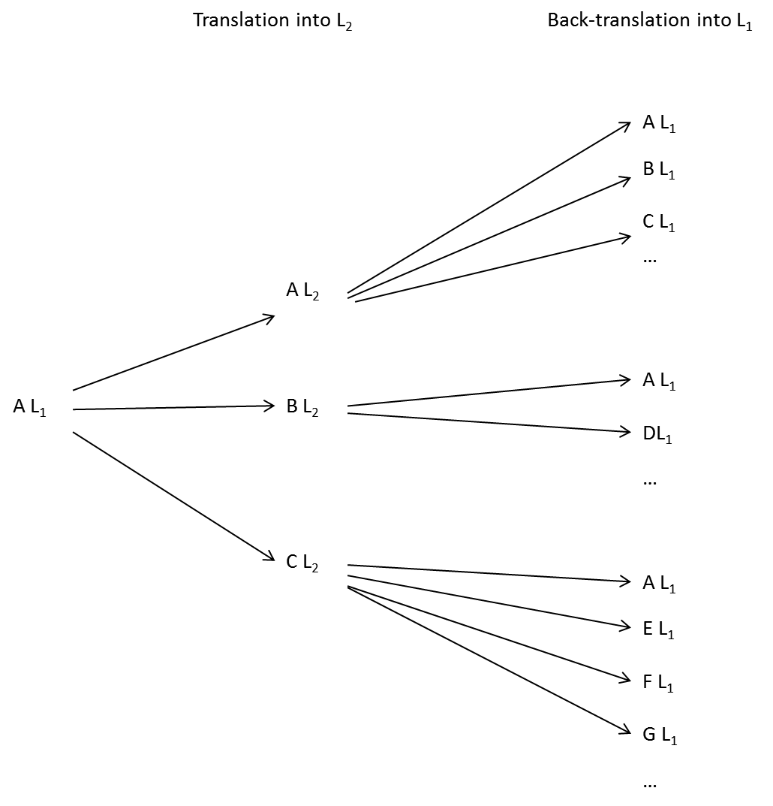
\includegraphics[height=.3\textheight]{figures/Vandevoorde2-img1.png}
\caption{\label{fig:key:2}  Back-translation procedure for contrastive analysis \citep[478]{dirven_functionalism_1987}
}
\end{figure}

To resume, back-translation was initially developed by Ivir as a contrastive-linguistic tool or procedure to identify formal correspondents (redefined by Ivir as contrastive correspondents) within translational data, therefore relying on a usage-based relation of translation equivalence.

Two additional advantages of the technique need to be pointed out here. First, the procedure of back-translation enables the researcher to lay bare the one-to-many relationship between an L1 item under scrutiny and its L2 contrastive correspondents and can therefore possibly lay bare meaning differences:

\begin{quote}
The relationship between an L1 unit and its L2 correspondents is not one-on-one but one-to-many, with each L2 correspondent matching a particular segment of the meaning of the L1 unit but also introducing other meanings which the L2 units has in the set of oppositions in that language \citep[177]{ivir_translation-based_1983}.
\end{quote}

Second, Ivir’s concern with the distinction of contrastive correspondents equally allows the (translation studies) researcher to separate the “irrelevant differences that are due to the translator’s idiosyncrasies or motivated by particular communicative or textual strategies” \citep[7:17]{altenberg_recent_2002} from what Dyvik will call the Linguistically Predictable Translations. The back-translation procedure seems thus to be suitable for both (contrastive) research into meaning (based on translational data) as well as for (corpus-based) investigations of meaning in translation.

\subsection{Applying back-translation: Mutual Correspondence}
\label{sec:2.3.3}  
Within contrastive linguistics a consensus was reached about the fact that information from translation corpora could be used as “an empirical basis for semantic claims” \citep[758]{noel_translations_2003}. According to \citet[24-28]{ebeling_patterns_2013}, back-translation formed the basis for using translational data and parallel corpora in contrastive analyses. Ivir’s work on back-translation has indeed been further used and developed within contrastive linguistics by, amongst other researchers, \citet{hasselgard_adverbial_1999} and \citet{altenberg_recent_2002}.

Altenberg and Granger’s application of back-translation is called Mutual Correspondence (henceforth MC; \citealt[254 ff.]{hasselgard_adverbial_1999}, \citealt[9]{altenberg_correspondence_2007}, \citealt[7:18]{altenberg_recent_2002}) and combines the idea of back-translation with a quantitative equivalence concept (such as Krzeszowski’s notion of statistical equivalence \citep[27-28]{krzeszowski_contrasting_1990}) in order to obtain more evidence about the relevance of the detected translation patterns \citep[17]{altenberg_recent_2002}.

\begin{quote}
‘Mutual correspondence’ (MC) is a simple statistical measure of the frequency with which a pair of items from two languages are translated into each other in a bi-directional translation corpus (see \citealt{hasselgard_adverbial_1999}). This can be calculated and expressed as a percentage by means of the formula:
\end{quote}

\begin{quote}\todo[inline]{Add missing equation}\end{quote} 

\begin{quote}
where A\textsubscript{t} and B\textsubscript{t} are the frequencies of the compared items in the translations, and A\textsubscript{s} and B\textsubscript{s} their frequencies in the source texts. The value will range from 0 (no correspondence) to 100 (full correspondence) \citep[9]{altenberg_correspondence_2007}.
\end{quote}

MC exploits Ivir’s notion of formal correspondence – established via back-translation – while adding a quantitative aspect to it. \citet{de_los_angeles_gomez_gonzalez_causative_2008} praises the possibility offered by back-translation “to control for translation effects” (“translationese”, cf. \citealt{wollin_translationese_1986}) by taking into account the “ “inverted” \textit{equivalence}” \citep[186]{de_los_angeles_gomez_gonzalez_causative_2008} and uses MC as a cross-linguistic measure of equivalence between two words or constructions (Ibid.). \citet{mortier_semantic_2010} describes her use of MC as the establishment of “the degree to which source and target items correspond in the two languages” (\citep[410]{mortier_semantic_2010}. Both applications agree that MC is a contrastive measure which holds between different language items, not between same language items: one can only calculate an MC between an L1 item \textit{a} and an L2 item \textit{z}, or between an L1 item \textit{b} and an L2 item \textit{y}, but MC does not provide the researcher with any (direct) information about the monolingual relationship between the two L1 items \textit{a} and \textit{b}. Furthermore, the resultant correspondences are calculated for each of the contrastive pairs individually; the overall ‘network’ of relationships between the source language lexeme(s) and all attested translations stays somewhat out of the picture.

Although MC is an interesting application of back-translation for semantic research, it is, due to its clear contrastive nature, incompatible with the research objective of this book, which is to compare semantic field representations in translated and non-translated language, since such a comparison involves different representations of one language.

\subsection{Applying back-translation: Semantic Mirroring}
\label{sec:2.3.4} 
A second application of back-translation can be found within automatic thesaurus extraction. The semantic mirrors method (hence: SMM) was first introduced in 1998 as a solution for automatic thesaurus building and underwent further development within the project “From Parallel corpus to Wordnet” which was carried out at the University of Bergen (2001-2004) \citep[311]{aijmer_translations_2004}. The project explores the use of translational data as a basis for semantic research. Possible applications of the technique are the derivation of “large-scale semantically classified vocabularies for use in machine translation and other types of multilingual processing” \citep[51]{johansson_translational_1998} and later also the derivation of wordnet relations within the previously mentioned project \citep[311]{aijmer_translations_2004}. The idea of the SMM – which will be at the heart of the methodological tool I will propose – in fact finds itself at this crossroads of linguistic software development and lexical-semantic investigations. In this section, I will explore how the SMM can be a possible answer to the investigation of meaning relationships in translation.

\subsubsection{\label{sec:2.3.4.1}  Selecting translational data}
First, and in an effort to hold the balance between computational linguistic pragmatic solutions and a traditional lexical semantic reticence to use translational data, Dyvik (i) puts forward a number of strong arguments in favor of translation and (ii) focuses on what he calls the \textit{translational} \textit{relation}, a notion that will underpin his translation-driven technique for lexical semantic investigation, i.e. the SMM.

According to Dyvik, the semanticist first needs to get persuaded of the usefulness of translation for linguistic semantics. Apart from his argument that translation is a large scale activity, bringing about a multi-lingual perspective on lexical semantics, Dyvik additionally and convincingly argues that translation is a normal kind of linguistic activity within wich meaning is evaluated and that, as a consequence, this evaluation takes place without any kind of metalinguistic, philosophical or theoretical reflection \citep[51]{johansson_translational_1998}. Hence, the relations between the texts, which are the observable results of the translator’s evaluation of the meaning under scrutiny, can be considered as empirical evidence about semantic relatedness (Ibid.).

Exactly because translation is such a normal, omnipresent type of activity, the \textit{translational} \textit{relation} can be said to emerge “as epistemologically prior to more abstract and theory-bound notions such as ‘meaning’, ‘synonymy’ and ‘inference’ ” \citep[27]{langemets_translations_2005}. This assumption suggests that the translational relation between languages can be taken as “a theoretical primitive, […] a concept not to be defined in terms of other concepts, but assumed to be extractable from translational data by interpretive methods” \citep[27]{langemets_translations_2005}. Following Dyvik, we accept that the translational relation can indeed be ‘extracted’ from translational data. It is furthermore the impossibility to produce a “perfect” translation which makes translation so interesting for the semanticist:

\begin{quote}
Languages [...] are discrete structures, and meanings are entwined in the structures themselves. Therefore, during translation, things crack and snap, things disappear, and things are added, and there is hardly ever a unique correct solution to a translational task. Instead, actual translations provide a host of alternative approximations to the unattainable ideal, and this is a potential source of information: semantic insights may emerge from the way the sets of alternatives are structured \citep[28]{langemets_translations_2005}.
\end{quote}

\subsubsection{Translationally derived features}
\label{sec:2.3.4.2}  
Convinced about the acceptability of the use of translational data, Dyvik’s first concern when working with this type of data is to select the \textit{adequate} data \citep[52]{johansson_translational_1998}: the contribution of contextual factors should be separated from the correspondence relations, the latter being the type of relations the (contrastive) semanticist is interested in. For this reason, (translational, parallel) corpus data cannot be used in their raw form: “bad translations” need to be filtered out of the data and so-called Linguistically Predictable Translations\footnote{A Linguistically Predictable Translation is a translation that is not (completely) dependent on “the particular text and its circumstances” \citep{johansson_translational_1998}. E.g. the translation of Dutch \textit{huis} in the source language sentence \textit{hij} \textit{woont} \textit{in} \textit{een} \textit{mooi} \textit{huis} [he lives in a beautiful house] by English \textit{house} in the target language sentence \textit{he} \textit{lives} \textit{in} \textit{a} \textit{beautiful} \textit{house} is linguistically predictable. On the other hand, the translation of \textit{huis} in the sentence \textit{ieder} \textit{huisje} \textit{heeft} \textit{zijn} \textit{kruisje} [every house has its crucifix] by \textit{cupboard} in the target language sentence \textit{there’s} \textit{a} \textit{skeleton} \textit{in} \textit{every} \textit{cupboard} is not linguistically predictable because it depends on the particular context, in this case, the idiomatic expression in which it is used.} need to be isolated from the totality of the data (Ibid.); the latter ones are consequently selected for further analysis. Dyvik’s decision to select LPTs is driven by the same concern as Ivir’s selection of contrastive correspondents (“how much of the translated material can the contrastive analyst use”). Dyvik arrives at the selection of the LPTs by applying a procedure which is very similar to that of Ivir’s back-translation. The difference between the two proposals lies in the purpose for which they apply back-translation: where Ivir’s sole concern is to select contrastive pairs, Dyvik moreover aims to generate new, semantically informative information (about synonymy, hyponymy, etc. to suit his thesaurus building purposes), and he does so by applying the method to a parallel corpus.

The semantic informativity of the procedure can be understood as follows. Consider, for example\footnote{This example is adapted to the Dutch-English language pair from Dyvik’s (\citeyear[29-31]{langemets_translations_2005}) German-English example.}, the Dutch noun \textit{heks,} which can be translated into English as \textit{hag} and \textit{witch.} According to Dyvik, the fact that alternative translations exist, points towards a relatedness to either different ‘aspects’ or different sub-senses of the meaning of \textit{heks}: each of the English words indicates one of the many possible ways of dividing the semantic potentiality of \textit{heks} \citep[31]{langemets_translations_2005}.

\begin{figure}
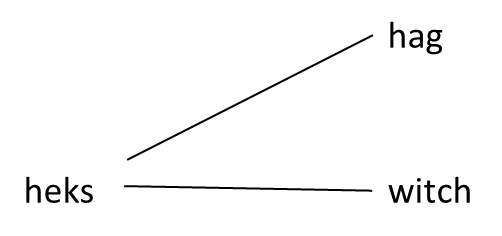
\includegraphics[height=.3\textheight]{figures/Vandevoorde2-img2.png}
\begin{forest} for tree={grow=east}
[heks [witch] [hag] ]
\end{forest}
\caption{\label{fig:key:3}  Translational correspondence}
\end{figure}

Subsequently, the lexical sub-senses of \textit{heks} could be expressed as contrastive pairs: <heks, hag>, and <heks, witch>. Within a translational approach, these \textit{pairs} (called \textit{sets} when several languages are involved) can be seen “as a kind of \textit{semantic} \textit{features}, [...] assignable to lexical items, both to the items they were derived from, and to others, which may inherit them [...]” (\citealt[31]{langemets_translations_2005}, our emphasis). Schematically, the “translationally derived features” would then look as follows:

\begin{figure}
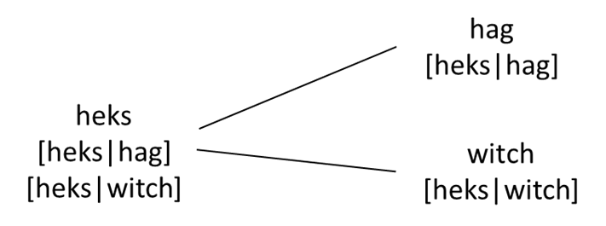
\includegraphics[height=.3\textheight]{figures/Vandevoorde2-img3.png}
\begin{forest} for tree={grow'=east,align=center}
[ heks\\{[}heks|hag{]}\\{[}heks|witch{]} [hag\\{[}hegs|hag{]}] [witch\\{[}heks|witch{]}]  ]
\end{forest}
\caption{\label{fig:key:4}  Translationally derived features}
\end{figure}

To sum up, semantic information can be obtained from \textit{translationally} \textit{derived} \textit{features}:

\begin{quote}
Intuitively, the features encode subsenses that the lexical items share with each other. In this way the features become \textit{classificatory} \textit{devices}, grouping lexical items together according to shared semantic properties (\citealt[31]{langemets_translations_2005}, our emphasis).
\end{quote}

In a classical structuralist approach, the semanticist would describe word meaning via a \textit{componential} \textit{analysis}, in which he assigns \textit{semantic} \textit{features} to words, in order to understand their interrelations \citep[28]{langemets_translations_2005}. While it is true that from a purely structuralist point of view translations could never be used as contrastive semantic informants – because different languages carve up the world or a same semantic field in different ways – Dyvik observes that these differences in carving up the same field are reflected “in the fact that this translational relation is not one-to-one” (Ibid., 29) and are semantically informative: contrastive differences can be a reflection of difference(s) (in classification) of semantic properties. Dyvik explicitly states that meaning can be inferred from the \textit{translational} \textit{relation} between a source language (lexeme/structure) and its translation:

\begin{quote}
Corresponding sets of terms in two languages are connected by a relation of translation \citep[29]{langemets_translations_2005}.
\end{quote}

\begin{quote}
The translational relation between the signs of two languages (interrelating ‘linguistically predictable translations’) is an instance of the sharing of meaning properties across languages \citep[217]{hasselgard_complexity_1999}.
\end{quote}

In other words: a \textit{translational} \textit{relation} cannot exist between an LPT and its source language lexeme if these two do not share any meaning properties \citep[218]{hasselgard_complexity_1999}. Translational properties can be ‘easily’ accessed – at least more easily than the much more abstract meaning properties – by investigating source texts and their translations. It can therefore be tried to “define (some) meaning properties in terms of translational properties rather than the other way around (as is common)” \citep[218]{hasselgard_complexity_1999}. In Dyvik’s view – which will adopted for the extension of the SMM (see \sectref{sec:3.4}) \textbf{–} semantic features can be derived from translational data\textbf{:} alternative translations are related to different aspects or related sub-senses of the meaning of a word under scrutiny \citep[31]{langemets_translations_2005}, and can divide up the semantic potentiality of the given word (Ibid.). In this way, “sets of translationally corresponding items across languages [can be seen] as \textit{the} \textit{primitives} \textit{of} \textit{semantic} \textit{descriptions}” (Ibid.), and the contrastive pairs can be considered as semantic features, assignable to lexical items (Ibid.).

\subsubsection{Ivir and Dyvik} 
\label{sec:2.3.4.3}  
Although Dyvik’s mirroring method shows quite some resemblances to Ivir’s ideas about contrastive correspondents and back-translation, Dyvik seems to develop his method independently of Ivir’s previously established notions. Dyvik’s and Ivir’s proposals are similar in that they (i) each use a mechanism which allows them to select only those translational data which they find suitable and ‘safe’ for contrastive analysis; and (ii) treat the relation of translational correspondence as a symmetric relation “disregarding the direction of translation” \citep[314]{aijmer_translations_2004}, a viewpoint which is in line with their research goal and seems for both Ivir and Dyvik the methodologically right thing to do: in their contrastive view, pairs of translations are informative tools used for their dynamics to move between languages in a meaning-preserving way, informing the researcher about meaning, while the influence of the task of translation itself is brought down to a minimum, so that the data are as contrastively pure as possible. From a point of view of translation studies though, the translational relation is clearly asymmetric and this has been proven via the same practice of back-translation: “[m]ultiple examples from the practice of back translation have proven that translation pairs are not symmetric and translation through several languages make the lack of transitivity similarly apparent (see e.g. Levý 1989)” \citep[211]{halverson_concept_1997}. Since the current study focuses on translation itself, and not merely on its exploitation as a (logical) tool, the asymmetry of the translational relation will necessarily have to be taken into account.

One could wonder why such an effort is made here to present Dyvik’s technique, if in fact Ivir’s previously formulated ideas were so similar. There are several important reasons to prefer the SMM to Ivir’s ‘pure’ back-translation as a basis for this methodological tool. First, Dyvik makes an important link between a technique, back-translation, and a specific research objective: lexical semantic research, an objective which I share with Dyvik. As a matter of fact, Dyvik operationalizes Ivir’s intuition that each L\textsubscript{2} correspondent will be related to a number of other L\textsubscript{1} items too, besides the L\textsubscript{1} with which the analysis was initiated \citep[478]{dirven_functionalism_1987} by retrieving the “other L\textsubscript{1} items” in an additional corpus-based retrieval step (called the inverse T-image). Second, as \citet[25]{ebeling_patterns_2013} rightly remark, Ivir never explains the procedure of back-translation in detail, which makes it difficult to know whether he applies the method with a parallel corpus or if back-translation is done on the basis of the analyst’s translational intuitions. For Dyvik on the contrary, the use of (parallel) corpora is an obviousness, explicitly mentioned in his design. Again, I share Dyvik’s view to explicitly put forward a parallel corpus approach for research in lexical semantics of translation. Finally, Dyvik further develops and exploits a notion (which was also mentioned by Ivir, but not exploited) i.e. \textit{overlap} to ensure the semantic relatedness between the yielded lexemes. Overlap is part of the procedure of back-and-forth translation, and forms an additional dimension which will be used in the extended version of the SMM (see \sectref{sec:3.4}).

\subsubsection{The SMM in contrastive linguistic studies}
\label{sec:2.3.4.4} 
Within contrastive, corpus-based studies, Aijmer and Simon-Vandenbergen have drawn extensively on Dyvik’s idea of using translations as “mirrors” in semantic field research. They mainly focused on discourse particles \citep{simon-vandenbergen_english_2013}, pragmatic markers \citep{simon-vandenbergen_expectation_2002-2003,aijmer_model_2004,fischer_pragmatic_2006} and adverbs \citep{simon-vandenbergen_semantic_2007,simon-vandenbergen_english_2013}\footnote{\citet{mortier_adversative_2009} were inspired by the work of Aijmer and Simon-Vandenbergen and carried out a “mirror-analysis” for adversative discourse markers. Mortier \& Degand combine different types of corpora (parallel and comparable, with written and spoken data) to arrive at a “semantic profile” for the discourse markers under study. They emphasize that their application of the “mirror analysis” serves to establish “the field of formal equivalents in one language or across languages” \citep[309]{mortier_adversative_2009}. According to the researchers, a mirror analysis “consists of back-and-forth translations of a given item from the source language to the target language, and from the target language back to the source language”. Their application of the procedure in fact answers perfectly to Ivir’s \textit{back-translation} procedure for the retrieval of \textit{formal} \textit{correspondents} (and this is also the goal of Mortier and Degand), so their method stands much closer to Ivir’s contrastive notion than to Dyvik’s lexical-semantic tool.} . In line with the cautiousness which contrastive researchers usually show when employing translational data, Aijmer and Simon-Vandenbergen relied on Dyvik’s argumentation to legitimately incorporate the supplementary information which translations are able to provide about semantic similarity into their analysis. They show an interest in using the back-and-forth translations as a \textit{tertium} \textit{comparationis} (\citealt[16]{simon-vandenbergen_expectation_2002-2003}, \citealt[1795]{aijmer_model_2004}), but their main interest in Dyvik’s proposal stems from its aptitude to construct and compare semantic fields (\citealt[1131]{aijmer_discourse_2003}, \citealt[1782]{aijmer_model_2004}, \citealt[13]{simon-vandenbergen_expectation_2002-2003}). A number of adaptations and specifications are made by Aijmer and Simon-Vandenbergen to Dyvik’s original method:

Firstly, Aijmer and Simon-Vandenbergen always use at least three languages; i.e. the language under study (English) and two mirror languages: either Dutch and Swedish \citep{aijmer_model_2004}, or Dutch and French \citep{simon-vandenbergen_english_2013} or even four mirror languages (Dutch, Swedish, French and German) at once \citep{simon-vandenbergen_semantic_2007}, whereas Dyvik uses two languages: one language under scrutiny and one pivot language. Aijmer and Simon-Vandenbergen in fact combine the resulting translations from two mirror analyses (a mirror exercise can only be carried out with one language at a time) into one resultant relational field. If, for instance, Dutch and Swedish are used as pivot languages, this double mirror allows them to compare the “overlapping translations back into English”. “Overlapping translations” are interpreted here as those translations back into English which are obtained as translations of both Swedish and Dutch source lexeme(s). The result is a set of English lexemes, overlapping\footnote{Note that this interpretation of overlap differs from the interpretation of the notion in this study (see \sectref{sec:3.3.3}).} between Dutch and Swedish. Aijmer and Simon-Vandenbergen compare in this way the number of identical translations (from Dutch or Swedish) into English yielded in what they call “the second translation image” \citep[1796]{aijmer_model_2004}, which corresponds to Dyvik’s step of the inverse T-image (see \sectref{sec:3.3.1}). Combining different mirror images into one result also implies that data are obtained from different corpora and need to be combined while staying comparable.

Secondly, whereas Dyvik’s “ranking of signs in a semantic field” is done “quite independently of frequency of occurrence”\footnote{“(except that a lexeme of course has to occur at least 32 times in the corpus in order to be a member of 32 subsets)” \citep[73]{johansson_translational_1998}.} and based on the “overlap relations among \textit{t}{}-images” \citep[73]{johansson_translational_1998}\footnote{Recall the quote at the beginning of this section, stating that overlapping first \textit{t}{}-images do not guarantee that two lexemes indeed pertain to the same field “since the shared L2 sign may be ambiguous between an ‘\textit{a}{}-sense’ and a ‘\textit{b-}sense’ with no close relationship between them” \citep[72]{johansson_translational_1998}. In order to ensure that two lexemes do pertain to the same field, Dyvik proposed the technique of back-and-forth translation up to the level of the \textit{second} \textit{T-image} (the necessity of the \textit{second} \textit{T-image} will be further explicated in the methodological chapter of this study).}, \citet{aijmer_model_2004} use frequency information to differentiate the items of a lexical set (obtained via a mirror analysis as translations of one particular marker in one language under scrutiny): 

\begin{quote}
Such paradigms or lexical sets show, for example, which translations are more frequent or prototypical, and which are less frequent or even ‘singleton’ translations \citep[1785-1786]{aijmer_model_2004}.
\end{quote}

The (relative) frequency information of correspondences is used to distinguish between prototypical equivalents and more context-bound correspondences \citep[8]{simon-vandenbergen_semantic_2007}, but frequency information is not as such integrated in the visualized results which represent the translation networks \citep[250-253]{simon-vandenbergen_semantic_2007}. The researchers choose to only consider salient correspondences in their translation network “in principle the five most frequent ones, though individual decisions had to be taken in view of the large differences in absolute and relative frequencies in separate tables” (Ibid., 248). This problem is a direct consequence of the fact that different corpora had to be combined for this application. Conclusively, Aijmer and Simon-Vandenbergen do not neglect frequency information, but the resultant contrastive translation networks are not (directly) based on the frequencies of the correspondences; the lines which link up the contrastive lexemes in the translation networks in fact only reflect cross-linguistic translation overlap\footnote{This \textit{modus} \textit{operandi} is further confirmed in \citet[93-94]{simon-vandenbergen_english_2013}, where the relation (within a ‘mirror analysis’) between French or Dutch equivalents and English lexemes is indicated by one cross if such a relation exists and two crosses is the relation was recorded more than once.}, which is a different kind of overlap from Dyvik’s notion. A distinction is made between full lines to mark the prototypical correspondences, and broken lines which show “correspondences which are not prototypical but [...] still recurrent enough to be included” (Ibid., 248).

To sum up, Aijmer and Simon-Vandenbergen propose a “translation-based variant of semantics based on data from translation corpora” \citep[7]{simon-vandenbergen_semantic_2007} for which they draw on Dyvik’s semantic mirrors method. Interesting adjustments to the technique consist in their use of multiple languages to arrive at a final semantic map as well as the integration of frequency information, although without statistically incorporating this information into the analysis.

\subsubsection{The SMM in other domains of linguistics}
\label{sec:2.3.4.5}  
The SMM has also drawn the attention of researchers in Natural Language Processing. \citet{ganter_conceptual_2005} have proposed to model the SMM with Formal Concept Analysis, using concept lattices to visualize semantic relatedness instead of the Venn diagrams proposed by Dyvik. \citet{elden_computing_2013} propose to visualize the semantic relations which come from semantic mirrors via Spectral Graph Partitioning. In addition to this, the SMM has been compared, within the realm of computational linguistics, with its ‘competing’ distributional techniques for automated thesaurus construction. \citet{butz_comparing_2011} concluded that “with respect to synonyms, [...] mirror translations provide a better filter than syntactic distribution similarity” (p.333). It is beyond the scope of this study to further comment on these computational applications, but the fact that the SMM has been applied both in more theoretical contrastive linguistic works on the one hand and in computational applications on the other at least shows that the ideas underlying the SMM have found support in both theory and in practice.

\subsection{Conclusion}
\label{sec:2.3.5}  
Back-translation is a technique that can be used as a contrastive linguistic tool. It enables the researcher to isolate formal correspondents (renamed and re-defined by Ivir as contrastive correspondents) and to detect semantic relationships between lexemes in one language. An application of back-translation via semantic mirroring offers – in theory – the possibility to investigate semantic relationships in translated and non-translated language. Although the SMM has indeed the potential to lay bare meaning relationships, a number of issues remain unsolved. First, a operationalizable notion of translation equivalence allowing for valid comparisons between translated to non-translated language is still to be defined. Both Dyvik and Ivir established equivalence on the basis of a symmetric notion of the translation relation, but the idea that equivalence is symmetric is incompatible with the viewpoint of CBTS which is taken in this book. Second, the SMM was originally a method for thesaurus building and is therefore not ‘equipped’ to carry out comparisons of the semantic relationships it lays bare amongst different language varieties. Thirdly, provided that the first two issues can be overcome, a theoretical framework within which those comparisons can be interpreted, is still missing. Solutions to each of these problems can be found within corpus-based semantics.

\section{Corpus semantics}
\label{sec:2.4}  
Various theoretical insights from different areas of corpus-based semantics are brought together in this section. These insights are needed to underpin the methodology which will be presented in \chapref{sec:3}. Three elements are still missing: (i) an acceptable notion of translation equivalence (applicable within the SMM and allowing an asymmetric translational relation), (ii) an insightful means to compare semantic relationships in translated and non-translated language and (iii) a theoretical framework within which such comparisons can be interpreted. Corpus(-based) semantics is an extremely vast area of research. I will therefore only touch upon those domains that are immediately relevant to theoretically underpin the three aspects cited above.

In the first part of this section (\sectref{sec:2.4.1}), I deal with the notion of translational equivalence as it was developed in Word Sense Disambiguation. By considering translational equivalence according to its WSD-based definition, the notion can also be used when the translational relation is not considered symmetric (as is the case in this study).

In \sectref{sec:2.4.2}, I will show that the semantic relationships revealed on the basis of the translational equivalence hypothesis can be understood in terms of distances and captured in so-called Semantic Vector Spaces. Statistical visualization methods can consequently be used as “an intuitive interface” \citep*[17]{heylen_looking_2012} to study semantic relationships in fields of translated and non-translated language.

In \sectref{sec:2.4.3}, I will explore how the idea of a “prototype model of category structure” – considered as one of the important contributions of cognitive semantics to the study of word meaning \citep[577]{allan_lexical_2013} – can form the theoretical background against which the semantic relationships within the semantic field under study can be interpreted.

\subsection{Translational equivalence in Word Sense Disambiguation}
\label{sec:2.4.1}  
The idea that a procedure such as back-translation based on translation equivalence introduced in \sectref{sec:2.3} can be used to lay bare semantic relationships also exists within corpus-based semantics. The derivation of semantic relationships on the basis of translational equivalence is put into practice within Word Sense Disambiguation – a name commonly given in the field of computational linguistics to the task of “computationally determining which “sense” of a word is activated by the use of the word in a particular context” \citep[1]{agirre_word_2007}.

In WSD, unsupervised corpus-based methods\footnote{The different approaches to WSD are classified according to their main source of information: knowledge-based methods use sources such as dictionaries and thesauri, unsupervised methods collect information from raw unannotated corpora and include methods using word-aligned corpora which extract cross-linguistic information; (semi-)supervised methods train from annotated corpora, or use them to seed in a bootstrapping process \citep[12]{agirre_word_2007}.} are either based on the distributional hypothesis, or, alternatively, on the idea of translational equivalence \citep{agirre_word_2007}. So-called distributionalist methods are often summarized in John R. Firth’s well known words “You shall know a word by the company it keeps” \citep[11]{firth_synopsis_1957}\footnote{In computational linguistics, the distributional hypothesis is also commonly attributed to \citet{anscombe_philosophical_1953}, \citet{harris_distributional_1954}  or \citet{weaver_translation_1955} \citep[142-143]{turney_frequency_2010}.}.The translation equivalence hypothesis is based on the idea that a word can be known by the translational company it keeps. Translational equivalence methods were introduced into computational linguistics because of their relevance for machine translation \citep[134]{agirre_unsupervised_2007}, one of the earliest fields of application of WSD. The reliability of translational equivalence has received direct evidence from WSD: according to \citet[1]{ide_automatic_2001} “sense distinctions derived from cross-lingual information correspond to those made by human annotators, especially at the coarse grained level” and “the reliability of sense assignments at finer-grained levels is comparable for human annotators and those produced automatically with cross-lingual data”.

While in lexical semantics, distributional approaches are widely applied\footnote{In lexical semantics and lexical variation studies (e.g. \citealt{peirsman_automatic_2010}), the distributionalist idea has led to the advent of (semi-)automatic retrieval methods of semantically similar words such as latent semantic analysis \citep{landauer_solution_1997} first and second order bag-of-words models \citealt{manning_foundations_1999} and the behavioral profiles method \citealt{divjak_ways_2006, evans_behavioral_2009}.}, methods that rely on translational equivalence as a meaning-structuring device have not yet had much uptake. Admittedly, the distributional hypothesis has opened the way to a myriad of methodological possibilities and fine-grained analytical tools (which do not seem to have reached their limitations yet) so the ‘need’ to rely on an alternative hypothesis can seem somewhat obsolete. However, if one is interested in investigating the semantics of translated language (in comparison to non-translated language), the translational hypothesis might be an appropriate starting point. In fact, the idea of translational equivalence can be rather straightforwardly related to the widely used distributional approach. We could easily reformulate the acceptability of translational equivalence in distributionalist terms, i.e. with respect to the (additional or alternative) contextual disambiguation possibilities that translations offer: the addition of information from a second language (a translation) about a lexeme under scrutiny (the source language lexeme) – which stands in a translational relation to that lexeme – can be seen as ‘addition of context’. Translational equivalence methods could therefore be said to form – at least conceptually, and at least for research focusing on lexical semantic investigations in translation studies – a possible alternative for or addition to the existing distributional methods, as is already the case within WSD.

Now that we have argued in favor of the conceptual acceptability of translational equivalence for lexical semantic research in translation, we need to understand exactly how translational equivalence works within WSD. WSD methods based on translational equivalence unsurprisingly use translations as information source for disambiguation:

\begin{quote}
methods based on translational equivalence rely on the fact that the different senses of a word in a source language may translate to completely different words in a target languages \citep[134]{agirre_unsupervised_2007}
\end{quote}

In machine translation (the field where WSD researchers initially got the idea for translational equivalence), “the ambiguity of a source word is [...] given by the number of target representations for that word in the bilingual lexicon of the translation system” \citep[132]{dagan_two_1991}. For example, if in a machine translation task, the correct sense of the English lexeme \textit{bank} needs to be selected, the \textit{conditio} \textit{sine} \textit{qua} \textit{non} to perform this task (correctly) is that the system disposes of the necessary information to differentiate between the different senses of \textit{bank.} The distinctive senses of \textit{bank} can be assigned to the lexeme “by producing all the [French] alternatives for the lexical relations involving [bank]” \citep[131]{dagan_two_1991}. The French translation \textit{banque} distinguishes the “financial institution” sense of \textit{bank}, whereas the French \textit{rive} reveals the “riverside” sense of \textit{bank.} Schematically, the sense assignment looks as follows:

\begin{figure}
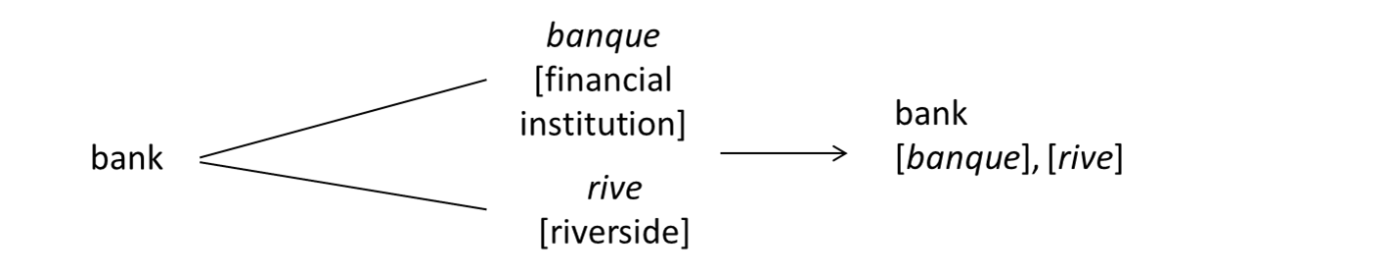
\includegraphics[height=.3\textheight]{figures/Vandevoorde2-img4.png}
\begin{forest}for tree={grow=east,align=center}
    [bank  [\textit{rive}\\{[}riverside{]}] [~~~~~~~~~~~~~~~~~~~~,name=dummy,no edge [bank\\{[}\textit{banque}{],} {[}\textit{river}{]},base=center,edge=->]] [\textit{banque}\\{[}financial institution{]}] ]
\end{forest}
\caption{\label{fig:key:5}Different senses of the English lexeme \textit{bank} are assigned based on its French translations}
\end{figure}

Given that the lexeme \textit{bank} now disposes of two possible senses, it has become possible to select the sense “which corresponds to the most plausible [French] lexical relations” \citep[131]{dagan_two_1991} and consequently to select the contextually correct target word.

Not all ambiguities can be resolved through ‘simple’ translational equivalence. For instance, at least two senses of the Dutch lexeme \textit{school} cannot be disambiguated while using English translations: the “educational institution” sense of Dutch \textit{school} translates in English as \textit{school,} and also the “group of fishes” sense of Dutch \textit{school} translates into English as \textit{school,} hence, ambiguity remains unresolved (\figref{fig:key:6}). In these cases, it is proposed to add a third language \citep[132]{dagan_two_1991}. In this particular case, adding French would help, as the “group of fishes” sense translates in French as \textit{banc,} and would reveal this additional sense (\figref{fig:key:7}).

\begin{figure}
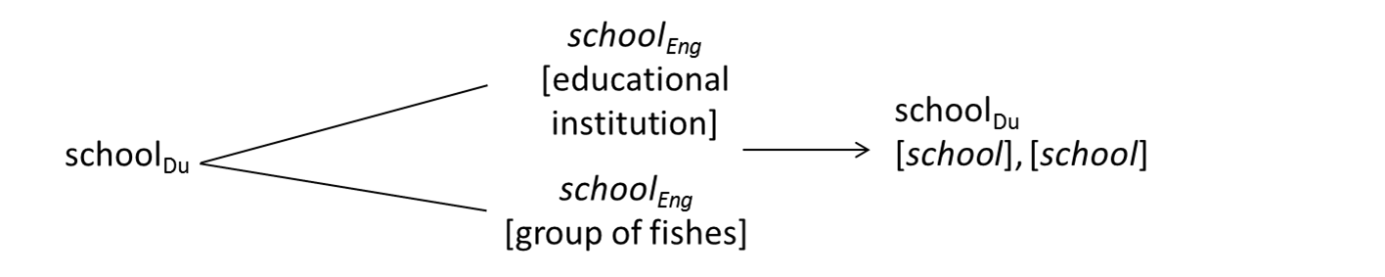
\includegraphics[height=.3\textheight]{figures/Vandevoorde2-img5.png}
\begin{forest} for tree={grow=east,align=center}
[school\textsubscript{Du} [\textit{school}\textsubscript{Eng}\\{[}group of fishes{]}] [~~~~~~~~~~~~~~~~~~~~,name=dummy,no edge [school\textsubscript{Du}\\{[}\textit{school}{],} {[}\textit{school}{]},base=center,edge=->]]  [\textit{school}\textsubscript{Eng}\\ {[}Educational institution{]}] ]
\end{forest}
\caption{\label{fig:key:6}Unresolved disambiguation via one language}
\end{figure}

\begin{figure}
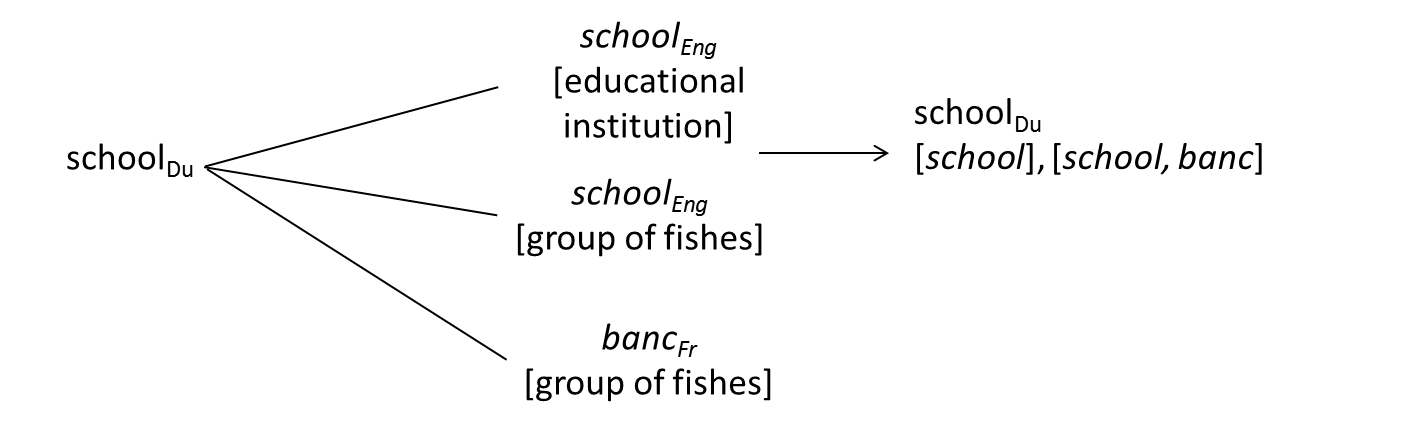
\includegraphics[height=.3\textheight]{figures/Vandevoorde2-img6.png}
\begin{forest} for tree={grow=east,align=center}
[school\textsubscript{Du}\\\vphantom{jh}~ [\textit{banc}\textsubscript{Fr}\\{[}group of fishes{]}] [\textit{school}\textsubscript{Eng}\\{[}group of fishes{]},base=center [school\textsubscript{Du}\\{[}\textit{school}{],} {[}\textit{school, banc}{]},base=center,edge=->]]  [\textit{school}\textsubscript{Eng}\\ {[}Educational institution{]}] ]
\end{forest}
\caption{\label{fig:key:7}Resolved disambiguation via two languages}
\end{figure}

While adding a language or even several languages \citep{gelbukh_five_2013}, has proven to be an effective way to enhance the WSD procedure, it is also conceptually possible to rely on a single language and still arrive at the disambiguation of the different senses. This can be done by applying the procedure of back-and-forth translation following the SMM. Within the SMM, the translational relation is, however, considered as symmetric, an idea which is incompatible with my point of view that translation is necessarily asymmetric (see \sectref{sec:3.4.1}). The idea of a symmetric translation equivalence relation is, however, not a prerequisite to carry out back-and-forth translation with the SMM. In fact, disambiguation via the SMM can rely on the same basic idea as disambiguation via several languages in WSD, which states that the different senses of a word are determined by considering only those distinctions that are lexicalized cross-linguistically \citep[54]{agirre_making_2007}. By considering the relation of translational equivalence in the SMM as identical to the one in a WSD disambiguation task with several languages, i.e. not necessarily symmetric and lexicalized cross-linguistically – the SMM can be used for the disambiguation task carried out in this study.

\subsection{Vector Space Models}
\label{sec:2.4.2}  
The SMM can be used to reveal semantic relationships, but it cannot be “readily” used to compare the obtained relationships amongst different language varieties. The same holds for WSD: it is a (computational) task to determine sense distinctions, but it does not offer solutions as to how the disambiguated senses can be objectively compared to each other. Objective comparisons would indeed require objective visualization methods, which neither the SMM nor WSD straightforwardly offer. In this section, I will turn to linguistic semantics and corpus-based cognitive semantics, which are mainly occupied with the empirical study of lexical meaning. Semantic relationships revealed on the basis of the translational equivalence hypothesis can be understood in terms of distances and captured in so-called Semantic Vector Spaces (SVS). Statistical visualization methods can consequently be used as “an intuitive interface” \citep[17]{heylen_looking_2012} to explore the semantic relationships in fields of translated and non-translated language “captured by an SVS” (Ibid.).

In linguistic semantics and corpus-based cognitive semantics, the perceived difficulties to introspectively analyze meaning and meaning differences have led to the development of “a methodology for empirical research in cognitive linguistics that is based on thorough quantitative analysis of corpus data” \citep[91]{kristiansen_methodological_2008}. Data are derived from or gathered via corpora and quantitatively analyzed using methods that are “methodologically similar” to work in computational linguistics or information retrieval \citep[6]{gries_introduction_2006}. \citet[242]{riemer_sense_2016} and \citet{glynn_empirical_2010} discern three major perspectives: experimental research, the referential method and the distributional, corpus-based approach. My own proposition to reveal semantic relationships on the basis of the translational hypothesis can be fitted in with the distributional, corpus-based approaches to the empirical study of lexical meaning as translations can be considered as an alternative for or additional type of context.

The distributionalist corpus-based method takes three main forms \citep[242-243]{riemer_sense_2016}: one in the tradition of Sinclair, a second one following the behavioral profile approach and a third form, called the semantic vector space approach. In Sinclair’s tradition, statistical methods are used to “identify semantically relevant contextual clues in the corpus” \citep[242]{riemer_sense_2016} after which the “semantic characterization” of the words and expressions is usually analyzed manually (Geeraerts, Ibid.). The behavioral profile approach takes the opposite direction: potentially interesting features are first tagged manually or semi-automatically, after which statistical techniques are applied to “classify the occurrences into distinctive senses and usages” \citep[243]{riemer_sense_2016}. Various statistical techniques have been used within this approach, e.g. hierarchical cluster analysis by \todo{REF unclear}\citet{Gries2006b} and \citet{divjak_structuring_2010} and correspondence analysis by \citet{glynn_empirical_2010} \citep[243]{riemer_sense_2016}. The third approach discerned by Geeraerts, the semantic vector space approach, uses quantitative techniques on both levels: contextual clues are first identified in a statistical way; the subsequent “clustering of occurrences on the basis of those clues” is equally carried out statistically \citep[243]{riemer_sense_2016}.

Vector Space Models (hence: VSMs) – which are put forward within this semantic vector space approaches – were initially proposed as a solution to the problem of document retrieval in Information Retrieval \citep[495]{lappin_vector_2015}. They can be combined with the distributional hypothesis “as an approach to representing some aspects of natural language semantics” \citep[141]{turney_frequency_2010}. \citet[212]{szmrecsanyi_semantic_2014} explain how VSMs can be combined with the distributional hypothesis:

\begin{quote}
[I]n Vector Space Models, objects are described by \textit{n} quantifiable characteristics. These characteristics make up an n{}-dimensional space in which the objects can be positioned. Every characteristic is thus a dimension. The position of the objects along these dimensions depends on the value that the characteristics have. In a way, these values can be seen as coordinates of a point in the \textit{n}{}-dimensional space, made up by the characteristics. The values of a single point are stored in a so-called vector. Every vector represents the object that is described by its characteristics. The spatial idea that underlies Vector Space Models does not restrict the objects to tangible items. Indeed, in Distributional Semantics, word meanings are objects, and the characteristics are contexts in which these words appear \citep[212]{szmrecsanyi_semantic_2014}.
\end{quote}

When VSMs are combined with the distributional hypothesis, the quantifiable characteristics of the object (i.e. of the word meaning) are the contexts of the word under scrutiny. Parallel to this proposition, VSMs can now also be combined with the translational equivalence hypothesis: the quantifiable characteristics which make up an n-dimensional space are then the translations or the source language lexemes of a word under scrutiny provided that a relationship of translational equivalence has been established (which will be done via the SMM++) between the translation/source language word and the word under study.

The attraction of the VSMs for semantic research resides in the fact that they can be used to quantify semantic similarity “by applying the spatial idea that underlies the Semantic Vector Space Models” \citep[213]{szmrecsanyi_semantic_2014}. This works as follows:

\begin{quote}
If two objects are very close to each other in an \textit{n}{}-dimensional Semantic Vector Space, then they are bound to have very similar values on a number of dimensions. If two objects behave alike for a large number of characteristics, represented by the dimensions, they must be very similar to each other, with respect to these dimensions. Given that we assume that the dimensions in Semantic Vector Spaces represent the Distributional Semantics of a lemma, spatial closeness of two words translates into semantic similarity between these words” \citep[213]{szmrecsanyi_semantic_2014}.
\end{quote}

Again, the idea that Semantic Vector Spaces can be combined with the distributional hypothesis can be transposed to the translational hypothesis: in order to know how semantically similar two words are in translated and non-translated language, equally the spatial proximity between those two words can be measured in both varieties. For instance, the semantic similarity between stoel [chair] and bank [bench] can be measured in translated Dutch and compared to the semantic similarity between those same two lexemes in non-translated Dutch. In translated Dutch, stoel [chair] and bank [bench] are translations and each lexeme is represented by a vector containing all possible source language words obtained from a corpus (as frequency values). For non-translated Dutch, stoel [chair] and bank [bench] are source language lexemes and each lexeme is represented by a vector containing all possible translations obtained from a corpus (as frequency values). Following the idea that “spatial closeness of two words translates into semantic similarity between these words” \citep[213]{szmrecsanyi_semantic_2014}, we can compare the distances between stoel [chair] and bank [bench] in both varieties and consequently compare the semantic similarity between the two lexemes for both translated and non-translated Dutch. 

In a large, corpus-based study such as this one, each translation or source language lexeme will be represented as a row in a frequency table and each characteristic of the n-dimensional space (source language lexeme or translation) will be represented as a column variable in a data matrix. If one wants to see “what kind of semantics” \citep[17]{heylen_looking_2012} is hidden within such potentially huge data matrices “an intuitive interface to explore the semantic structure captured by an SVS” (Ibid.) will be needed. Such an interface (a visualization) can then be obtained via statistical analysis of those data matrices. In this study, Correspondence Analysis and Hierarchical Cluster Analysis will be applied to yield such visualizations (see \sectref{sec:3.6}).

\subsection{Corpus-based cognitive semantics}
\label{sec:2.4.3}  
In linguistic semantics, thorough quantitative corpus analyses have been combined with theoretical concepts of cognitive linguistics, mostly in an attempt to arrive at a more empirical account of lexical meaning. Heylen et al. compared the work developed by two groups of researchers who have “relatively independently [developed] the methodology of “cognitive linguistically inspired” quantitative corpus analysis” \citep[92]{kristiansen_methodological_2008}\footnote{The comparison between the two approaches will not further be discussed here, but see: \citet{kristiansen_methodological_2008}. Briefly, the differences between the approaches situate themselves on the level of the phenomena under investigation, explanatory approaches and the exact statistical technique employed \citep[92-93]{kristiansen_methodological_2008}.}. \citet{Gries2006b}\todo{REF unclear} explains that, by bridging the gap between cognitive studies and corpus-based studies, rather than focusing on the distributional characteristics of different word senses, it should become possible to be informed about “how different word senses are related” \todo{REF unclear}\citep[57]{Gries2006b}. The integration of a cognitive linguistic framework within a corpus linguistic study is moreover believed to lead to more “theoretical sophistication” \citep[16]{gilquin_corpus_2010}. In this section, a “prototype model of category structure” will be proposed as the theoretical basis for the interpretations of the obtained visualizations (see \chapref{sec:4}). The “prototype model of category structure” is considered as one of the important contributions that cognitive semantics has made to the study of word meaning \citep[577]{allan_lexical_2013}. In the first part of this section (\sectref{sec:2.4.3.1}), I will zoom in on the notion of prototypicality so that it can be used in an unproblematic way to further describe and interpret the results presented in the subsequent chapters of this study. In the second part (\sectref{sec:2.4.3.2}), I will show how Divjak’s proposal to opt for a prototype-based categorization for low-contrastive verbs expressing abstract concepts also seems to be the better choice for this study. In addition, I will comment on Divjak’s two proposals of internal category organization (schematic or radial structure). Just as Divjak, I will also prefer a radial category organization.

\subsubsection{A prototype-based view and prototype effects}
\label{sec:2.4.3.1}  
The development of prototype theory received its most important impetus from psycholinguistic research conducted by Eleanor Rosch and colleagues in the 1970s \citep{rosch_cognitive_1975,rosch_family_1975,Rosch1978}\todo{REF unclear}. One of Rosch’s most important findings was that “[m]ost, if not all, categories do not have clear cut boundaries” (\citealt[196]{margolis_principles_1999} [1978])\todo{Check cite format}. The idea of fuzzy category boundaries, seemed, however, not easy to connect to the ‘dictate’ of cognitive economy that saw categories as “being as separate from each other and as clear-cut as possible” (\citealt[196]{margolis_principles_1999} [1978])\todo{Check cite format}. Rather than intending to achieve cognitive economy via “formal, necessary and sufficient criteria for category membership”, one could, alternatively, opt to marry fuzzy boundaries with cognitive economy by “conceiving of each category in terms of its clear cases rather than its boundaries” (\citealt[196]{margolis_principles_1999} [1978])\todo{Check cite format}. Prototypes of categories are then “the clearest cases of pry membership defined operationally by people’s judgments of goodness of membership in the category” (Ibid.). Rosch thus considered perception of typicality difference and hence also degree of prototypicality as an empirically verified fact. Given this empirical fact, Rosch went on to ask precisely “what principles determine which items will be judged the more prototypical?” (\citealt[197]{margolis_principles_1999} [1978])\todo{Check cite format}. Her hypothesis was that “prototypes develop trough the same principles such as maximization of cue validity and maximization of category resemblance as those principles governing the formation of categories themselves” (Ibid.). Support for this hypothesis can be found in \citet{rosch_family_1975} who showed that “the more prototypical of a category a member is rated, the more attributes it has in common with other members of the category and the fewer attributes in common with members of the contrasting categories” (\citealt[197]{margolis_principles_1999} [1978])\todo{Check cite format}.

Outside the field of psycholinguistic research, Rosch’s findings have further evolved and influenced psycholexicology on the one hand, and from the mid-1980s onwards also (general) linguistics \citep[578]{allan_lexical_2013}. As far as cognitive linguistics is concerned, prototype theory is even seen as one of its cornerstones \todo{REF unclear}(\citealt[145]{Geeraerts2006}  [1989])\todo{Cite format}. According to Geeraerts, within linguistics, Rosch’s conclusions that “perceptually based categories do not have sharply delimited borderlines” developed into “a more general prototypical view of natural language categories, more particularly, categories naming natural objects” \citep[578]{allan_lexical_2013}. Geeraerts further summarizes the application of prototype theory to the domain of linguistics as follows:

\begin{quote}
The theory implies that the range of application of such categories is concentrated round focal points represented by prototypical members of the category. The attributes of these focal members are the structurally most salient properties of the concept in question; conversely, a particular member of the category occupies a focal position because it exhibits the most salient features \citep[578]{allan_lexical_2013}.
\end{quote}

According to Gilquin, the importance of the introduction of the notion of prototypicality in linguistic theory lies in the fact that categories do not ‘need’ to be described any longer by lists for necessary and sufficient properties, but can instead be described according to more central and more marginal category members \citep[160-161]{gilquin_place_2006}. Prototypicality was furthermore extended beyond concrete objects to more abstract categories such as past tense and syntactic constructions (\citealt{gilquin_place_2006}, referring to \citealt{taylor_linguistic_1989}).

The use of the notion within linguistic theory is, however, not uncontroversial. Geeraerts shows that prototypicality is itself “a prototypical notion with fuzzy boundaries” \todo{REF unclear}(\citealt{Geeraerts2006}[1989]). Prototypicality, according to Gilquin, needs to be considered as follows:

\begin{quote}
a multi-faceted concept, bringing together (1) theoretical constructs from cognitive literature and relying on deeply-rooted neurological principles such as the primacy of the concrete over the abstract, (2) frequently occurring patterns of (authentic) linguistic usage, as evidenced in corpus-data, (3) first-come-to mind manifestations of abstract thought, as revealed through elicitation tests and (4) possibly other aspects that contribute to the cognitive salience of a prototype \citep[180]{gilquin_place_2006}.
\end{quote}

By defining prototypicality along these different lines, Gilquin tries to incorporate the four hypotheses uttered by \citet{geeraerts_where_2006}  [1988] as possible answers to the question: “where does prototypicality come from?”. These four hypotheses run as follows: First, the physiological hypothesis: prototypicality is considered as the result of the physiological structure of the perceptual apparatus \citep{moore_internal_1973}. The problem with this hypothesis is that it is difficult to apply to concepts without physiological basis \citet[28]{geeraerts_where_2006} [1988]. Second, the referential hypothesis: prototypicality as the result of the fact that “some instances of a category share more attributes with other instances of the category than certain peripheral members of the category” \citet[28]{geeraerts_where_2006} [1988]. This hypothesis is also referred to as the “family resemblance model of prototypicality” \citep{rosch_family_1975}. The number of shared attributes among the objects, events,... a concept can refer to, can allow the researcher to compute differences in salience (\citealt[29]{geeraerts_where_2006} [1988]). Thirdly, according to the statistical hypothesis, the prototype is that member of a category which is most frequently experienced. \citet[29]{geeraerts_where_2006} [1988] adds that the second and the third hypothesis can be combined: one can ascribe weights to category attributes on the combined basis of family resemblance and relative frequency \citep{rosch_cognitive_1975}. Finally, the fourth hypothesis is the psychological (also called functional) hypothesis which states that “it is cognitively advantageous to maximize the conceptual richness of each category through the incorporation of closely related nuances into a single concept because this makes the conceptual system more economic” (\citealt[28]{geeraerts_where_2006} [1988]).

I follow Gilquin’s “multi-faceted” view on prototypicality, which incorporates Geeraerts four hypotheses. However, the following question arises: if a prototype-based view on language is taken and claims are made about the semantic relationships within the presumably prototype-based semantic fields, how can one be sure that the chosen method will actually render a prototype-based structure? Given the corpus-oriented scope of this work, the most straightforward way of ‘ensuring’ that the yielded semantic fields will be prototype-based is to integrate both Geeraerts’ second (family resemblance / salience) and the third (statistics) hypothesis. In this way, a cognitivist view on prototypicality – “cognitivists tend to consider the prototype as the cognitively most salient exemplar” \citep[159]{gilquin_place_2006} – is united with a corpus-linguistic view which usually considers the prototype as the most frequently corpus-attested item (Gilquin, Ibid.). As Gilquin points out, most of the time, both cognitivists and corpus-linguists assume that salience and frequency coincide with one another (Gilquin, Ibid.). Although Gilquin does not negate the role of frequency in prototypicality, she also cites \citet[36]{sinclair_corpus_1991} who argues that “for common words, as a rule, the most frequent meaning is not the one that first comes to mind”. In this study, I will not only take frequency as a measure of prototypicality, I will also propose a way to operationalize salience, and I will do so by taking into account the number of overlapping translations. By doing so, I also tackle the problem that “[t]he lack of convergence between salience and text frequency [could] challenge[ ] the ability of corpora to serve as a shortcut to cognition” \citep[9]{arppe_cognitive_2010}. By considering translations as attributes, I can apply Geeraerts idea (\citeyear[29]{geeraerts_where_2006} [1988]) that the number of shared attributes (overlapping translations) can be used to compute salience. The principle of overlap will be further developed in \sectref{sec:3.3.3}. In short, I combine the use of frequency – the statistical hypothesis – and overlap – my operationalization of salience – to determine the status (more prototypical or more peripheral) of the member(s) of the semantic field I plan to visualize.

Geeraerts’ four hypotheses can be linked to a number of prototype effects. Just as Rosch was interested in the principles governing prototypicality judgment, within linguistics too researchers felt the need to differentiate between different phenomena that were all linked in some way to prototypicality (or to one of the previously cited hypotheses about the origins of prototypicality) and consequently prefer to talk about prototype effects rather than about prototype theory \citep[578]{allan_lexical_2013}. Geeraerts sums up a list of four characteristics about which there exists a consensus in the literature on the fact that “these characteristics are prototypicality effects [...] may be exhibited in various combinations by individual lexical items, and [...] may have very different sources” \citep[578]{allan_lexical_2013}. The list of prototypicality effects is determined as follows by Geeraerts:

\begin{quote}
First, prototypical categories exhibit degrees of typicality: not every member is equally representative for a category. Second, prototypical categories exhibit a family resemblance structure, or more generally, their semantic structure takes the form of a radial set of clustered and overlapping readings. Third, prototypical categories are blurred at the edges. Fourth, prototypical categories cannot be defined by means of a single set of criterial (necessary and sufficient) attributes \citep[187]{geeraerts_theories_2010}.
\end{quote}

The existence of these prototypicality effects will need to be taken into account in the development of the methodology (see \chapref{sec:3}). Under the assumption that not every member is equally representative for a category, the method will need to be able to inform about member representativity (this will be done by calculating the distance from each lexeme to its cluster’s centroid, see \sectref{sec:3.6.3}). As far as the family resemblance structure is concerned, it will be integrated by means of the so-called overlap principle. The fuzziness of category boundaries will be dealt with by imposing a minimum threshold for the overlap criterion (see \sectref{sec:3.4.3}) and the remaining fuzziness will be evaluated by assessing the distance of each lexeme to its cluster’s centroid as well as to the centroids of other clusters (see \sectref{sec:3.6.3})). Lastly, the lexeme selection technique based on the SMM takes translations as its attributes – so categories do not need to be defined according to their necessary and sufficient attributes.

\subsubsection{A prototype-based categorization of verbs}
\label{sec:2.4.3.2} 
Divjak remarks that many of the experiments about prototype categorization have been conducted on nouns, so that “[e]xtending prototype categorization to verbs [...] presupposes that knowledge about structures pertaining to nouns might be operative in verbs” \citep[150]{divjak_structuring_2010}. Given a number of differences between nouns and verbs –verbs are not stable/ time independent, verbs name intangible events, verbs render relational concepts (Ibid.) – it is indeed plausible that “conceptual categories associated with verbs and adjectives function differently from those associated with nouns” (Ibid.). According to Divjak, verbs are in general more abstract concepts than nouns and therefore less tangible, making it more difficult to capture them in prototype representations (Ibid.). As far as the intangibility of the verb concepts is concerned, \citet[152]{divjak_structuring_2010} refers to \citet[114]{pulman_word_1983} who states that verbs will require “more complex and more abstract attributes” than more tangible concepts expressed by nouns (where the prototypical members are those which share most attributes with some members of a category and only some attributes with other, peripheral members). Despite these differences, Divjak indicates that there is “some psychological evidence that people categorize event-related and object-related information in a similar way” \citep[151]{divjak_structuring_2010}. There seems to be no doubt however that “categories for intangible relational concepts also display prototype effects” (Ibid., 153), as is shown by \citet{schmid_cottage_1993}, \citet{taylor_linguistic_1995,taylor_linguistic_2003} and \citet{geeraerts_preponderantieverschillen_1985, rudzka-ostyn_where_1988, geeraerts_homonymy_1990} \citep[153]{divjak_structuring_2010}. Divjak concludes that choosing categorization by prototype is “quite adequate for modeling low-contrastive verbs, expressing abstract concepts such as intention, attempt or result [...]” (Ibid., 150).

Since the semantic domain covered in this study also expresses a rather abstract concept (inchoativity), I believe that the above line of reasoning in favor of prototype-based categorization also holds for this study. Divjak herself uses ID tags to set up behavioral profiles for each of the verbs in her study for prototype identification \citep[158]{divjak_structuring_2010}. My own proposition to operationalize translations as attributes might offer an alternative solution to the ‘problem’ of the complexity of (abstract) verb attributes: an identical type of attributes can be assigned to nouns, verbs and adjectives alike, i.e. their corresponding translations (see \chapref{sec:3}).

A prototype-based organization for the internal structure of a category seems like a defendable choice; the next question that comes to mind is: what does it look like? \citep[149]{divjak_structuring_2010}. According to Divjak, “[w]ithin cognitive linguistics, complex categories are typically represented in one of two ways, i.e. as having a schematic or a radial structure” \citep[149]{divjak_structuring_2010}. The first way of representing complex categories follows Langacker’s idea of a “schematic network of interrelated senses” \citep[369,371]{langacker_foundations_1987}, where a schema is “an abstract characterization that is fully compatible with all the members of the category it defines” \citep[149]{divjak_structuring_2010}. The second way of representing complex categories is as a radial structure \citep[84]{lakoff_women_1987}: “[a] radial structure is one where there is a central case and conventionalized variations on it which cannot be predicted by general rules”. Although both types of categorization “are inherently related aspects of one and the same phenomenon and are often difficult to distinguish in practice” \citep[371 ff.]{langacker_foundations_1987}; quoted by \citep[149]{divjak_structuring_2010}, they are different in the sense that schematic networks require full compatibility with all the category members (a checklist of necessary and sufficient attributes), whereas radial category structures are prototype-based, implying that there are degrees of membership \citep[150]{divjak_structuring_2010}. Because of the compatibility of the radial category structure with the idea of a prototype-based organization of the internal structure, we will also aim to represent our visualizations as radial structures.

\section{Conclusion}
\label{sec:2.5}  
Empirical studies of meaning are rather scarce in CBTS. Within the translation universals paradigm, for example, the question whether universals exist on the semantic level too has not often been raised. This lack of empirical studies of meaning can be attributed to the typical status of meaning in translation, i.e. meaning as the invariant of translation. However, this alleged invariance of meaning cannot be accepted as a given since investigating meaning in translation could potentially answer the perennial question of the difference between translated and non-translated language. Universal tendencies such as levelling-out and normalization-shining through are well suited to investigate meaning relationships in translation and such studies could indeed even inform the universals research on an explanatory level.

In this Chapter, I put forward the semantic mirrors method, which uses translational corpora and integrates back-translation to arrive at a selection of lexemes pertaining to the same semantic field. The technique has the potential to lay bare meaning relationships while taking into account the distinction between translated and non-translated language.

With the prospect of elaborating a bottom-up statistical visualization method for semantic fields in translated and non-translated language, a number of theoretical notions from corpus-based semantics were further explored.

The envisaged method will contain the following elements: it will apply (a version of) the SMM, it will rely on a WSD-based interpretation of the notion of translational equivalence (making the concept operationalizable in a way that is acceptable for research in TS), it will rely on statistical visualization techniques that are usually employed in distributional semantics and it will take a prototype-based view on meaning to interpret the statistical visualizations.

In order to apply the SMM for this study, however, two practical issues still need to be solved. First, a way needs to be found in which the SMM can be applied to retrieve comparable sets of translated/target language on the one hand and sets of original/source language on the other hand. A clear distinction between those sets is of paramount importance, while comparability stays a prerequisite. A second point of attention which cannot be solved by merely applying the SMM is the objective visualization of the results: how to practically create the statistical visualizations of those retrieved sets of lexemes? These two issues will be at the center of the methodology described in the next chapter.
 
\chapter{Methodology}
\label{sec:3}

\section{Introduction}
\label{sec:3.1}  
In this methodological chapter, a technique to visualize semantic fields in translated and non-translated language will be developed. In the previous chapter, I introduced the SMM, a technique that was originally designed by \citet{johansson_translational_1998,langemets_translations_2005} to derive large-scale semantically classified vocabularies for machine translation and other kinds of multilingual processing. I concluded that this technique could potentially offer a methodological solution for meaning investigation in translation. In this chapter, I will further explore the SMM and see how the technique can now be employed to compare semantic relationships in translated and non-translated language. I will therefore propose two extensions to the SMM so that the technique can be used to both select (via bottom-up retrieval) and statistically visualize (by measuring the meaning relationships between the lexemes in terms of distances) sets of lexemes as representations of semantic fields of translated language and non-translated language. These visualizations then need to enable us to compare the created semantic fields to each other.

In \sectref{sec:3.2}, the distinction between onomasiology and semasiology will be presented. This distinction is important because it partially determines the interpretation of the visualizations. In \sectref{sec:3.3}, the corpus that will be used in this study, the Dutch Parallel Corpus, is described. In \sectref{sec:3.4}, I will give a detailed account of the SMM as it has been developed by \citet{johansson_translational_1998,langemets_translations_2005}. In \sectref{sec:3.5}, I will explain my own extensions of the technique. The first extension is an integration of translation direction and the asymmetry of translation into the retrieval task; the second extension focuses on how the output of the retrieval task can be used as an input for a statistical visualization of a semantic field. In \sectref{sec:3.6}, the first extension of the SMM will be applied to retrieve data sets for the semantic field of \textit{beginnen}/inchoativity in Dutch. In \sectref{sec:3.7}, the second extension of the SMM is applied via an exploration of a number of statistical methods that will allow for the visualization of semantic fields. In \sectref{sec:3.7.1}, a first visual exploration of the data on the basis of correspondence analysis is presented before, in \sectref{sec:3.7.2}, a hierarchical agglomerative clustering is carried out upon the output of the CA. This section also covers the choice of the distance measure (\sectref{sec:3.7.2.1}), clustering algorithm (\sectref{sec:3.7.2.2}) and number of clusters (\sectref{sec:3.7.2.3}) for the HAC. In the final part of this section (\sectref{sec:3.7.2.4}), I will compare the chosen procedure (CA on a HAC, Euclidean distance, Ward’s Minimum Variance Method) to alternative combinations of distance measures, clustering algorithms and spatial maps by assessing the overall strength of the cluster structures of those combinations.

In \sectref{sec:3.8} I present a methodological solution to investigate whether the presumed differences between translated and non-translated Dutch on the semantic level might be ascribed to levelling, shining through or normalization on the semantic level. The (changing) prototype-based organization of meaning distinctions within semantic fields of translated and non-translated Dutch and of lexemes within the meaning distinctions revealed by the clusters is based on the calculation of the distances of the clusters to the centroid of the semantic space and of medoids.

\section{Semasiological and onomasiological perspectives} 
\label{sec:3.2}  
In lexical semantics, a distinction is usually made between studies which take a semasiological outlook and others which take an onomasiological outlook on meaning \citep{geeraerts_structure_1994}. Semasiology takes the point of view of the different concepts which can be expressed by one word (the polysemy of a word); onomasiology takes the viewpoint of the different words that can be employed to express a single concept (near-synonymy). Given my choice to conduct this study on the most prototypical expression of inchoativity in Dutch, \textit{beginnen}, both a semasiological and an onomasiological outlook are possible.

A semasiological outlook implies that the intended visualizations are considered as possible and plausible representations of the different meanings of a word under study (in our case \textit{beginnen}). In this case, the representations of different meanings of a word are considered as a semantic map, “a representation of meanings or uses and the relations between them” (\citealt[23]{simon-vandenbergen_semantic_2007}, following \citealt{AusweraPlungian1998}). From an onomasiological point of view, the visualizations would represent the different ways of expressing one and the same concept under study (in our case, the field of inchoativity).

If one wants to discover the different words that can be used to express the concept of inchoativity (onomasiological viewpoint), the best option in a corpus study such as this one which typically does not give direct access to concepts but (only) to words, i.e. to lexicalizations of those concepts, would be to start with its most prototypical expression. On the other hand, the fact that this study starts off with a single word, i.e. \textit{beginnen}, simultaneously favors a semasiological outlook on meaning. If one wants to explore the different concepts expressed by \textit{beginnen}, the most logical choice would be to start this study with this lexeme itself. Hence, the choice of the initial lexeme \textit{beginnen} allows to take both a semasiological and an onomasiological outlook. I do acknowledge the necessity of distinguishing the two perspectives, although they are closely interwoven. \citet[30]{geeraerts_theories_2010} reminds us that “the semasiological extension of the range of meanings of an existing word is itself one of the major mechanisms of onomasiological change – one of the mechanisms, that is, through which a concept to be expressed gets linked to a lexical expression”. Therefore, the link between a lexical expression and a concept is always semasiological in one direction (from lexical expression to the (range of) concept(s)) and onomasiological in the other direction (from the concept to the (range of) lexical expressions).

The visualizations of semantic fields in this work will correspond to the visual output of a statistical analysis via Hierarchical Agglomerative Clustering (see \sectref{sec:3.7.2}). The different groupings (clusters) in a visual representation (dendrogram) will be considered as different meaning distinctions of the word under study. In particular, this means that each cluster in the dendrogram will be considered as a separate meaning (a meaning distinction) of the semantic field of the word under study, \textit{beginnen} (semasiological outlook). In addition, the lexical items which make up each cluster will be considered as the lexical expressions of the particular meaning distinction of the cluster they belong to (onomasiological viewpoint). It is also possible to take a broad onomasiological outlook and to consider each visualization (dendrogram) as a whole as a representation of a semantic field of inchoativity, represented by its (most prototypical) means of expression. The lexical items in the visualizations are then considered as lexical expressions of the central concept of inchoativity. This second option would imply that somewhat less importance is given to the meaningfulness – in terms of meaning distinctions of a central word – of the clustering: rather than considering the clusters as meaning distinctions of the central word, the clusters would ``simply'' indicate which lexemes are more near-synonymous expressions of the central concept. I choose to take a double semasiological-onomasiological outlook here: clusters are considered as meaning distinctions of the central word (semasiological outlook) and the lexical items in each cluster are considered as the expressions of the meaning distinction of the cluster (onomasiological outlook). By taking such a double view, the question can be raised whether the universal tendencies of translation are taking place on the semasiological level of the different meanings of a word (can the polysemy of a word be altered under the influence of translation?), or on the onomasiological level of the words expressing a particular meaning distinction (is the near-synonymy relation between different words altered under influence of translation?).

\section{The Dutch Parallel Corpus}
\label{sec:3.3}
All data for this study are drawn from the Dutch Parallel Corpus (DPC), which was developed as part of the STEVIN program. The primary goal of this program was “to set up an effective digital language infrastructure for Dutch, and to carry out strategic research in the field of language and speech technology for Dutch” \citep[1]{Spyns2013}. The DPC is a ten-million-word, sentence aligned, both parallel and comparable corpus (it is de facto a parallel corpus which can also be used as a comparable corpus). Within Laviosa’s\ia{Laviosa, Sara@Laviosa, Sara} terminological apparatus (presented in \sectref{sec:2.2.1.3}), the DPC can be described as a multi-source, parallel multilingual corpus. ``Multi-source'' since Dutch, French and English can all three be the source language of the texts in the corpus (and also the target language); ``parallel'' because the texts in one language are the originals of the translations in the other language; and ``multilingual'' because more than two languages are involved.

The DPC offers a number of indisputable advantages. With respect to corpus size the DPC is, to my knowledge and at the time of writing, the largest available parallel corpus of Dutch. It is furthermore balanced with respect to five text types (external communication, journalistic texts, instructive texts, administrative text, fictional and non-fictional literature) and four translation directions (Dutch to French, French to Dutch, Dutch to English and English to Dutch). Only for the text type literary texts, the corpus is not strictly balanced according to translation direction, but only according to language pair \citep[187]{spyns_dutch_2013}. The five text types on the so-called superordinate level are further subdivided into 19 basic levels, but the latter have “no further implications for the balancing of the corpus” \citep[378]{macken_dutch_2011}. Each text type accounts for 2,000,000 words and within each text type, each translation direction contains 500,000 words \citep[376--378]{macken_dutch_2011}. All text files consist of written text material (no data carriers other than text files are included), but no distinction is made in the DPC between “spoken” text material and “written” text material \citep[59]{delaere_translations_2015}, although available meta-data indeed allow the user to identify the spoken text material as such and to distinguish between texts “written to be read”, “written to be spoken” or  “written reproduction[s] of spoken language” \citep[59]{delaere_translations_2015}. It is important to keep in mind that the spoken text material in the DPC is categorized under the superordinate text type level administrative texts \citep[59]{delaere_translations_2015}, together with written text material. Divergent results for the text type administrative texts in a corpus study focusing on genre specific phenomena could thus be due to the invisible inclusion of this parameter into the text type. The DPC further offers the possibility to differentiate between “regional language varieties” \citep[48]{delaere_translations_2015} such as Belgian Dutch and Netherlandic Dutch, Belgian French and French French and British English and American English. It is also important to add that the DPC is built up of complete texts, not of samples and that the DPC is a ``closed'' corpus, meaning that no data are added any further to the corpus.

The DPC indeed fulfills all the prerequisites to be a representative corpus with regard to corpus size, content and types of text files (see \sectref{sec:2.2.1}). The corpus is aligned on the sentence level (the alignment was carried out by a combination of three alignment tools, see \citealt[190--191]{spyns_dutch_2013} for more details on the different tools, their advantages and drawbacks). The DPC is furthermore enriched with linguistic annotations such as part-of-speech tagging and lemmatization \citep[191]{spyns_dutch_2013}. With regard to lemmatization, \citet[384]{macken_dutch_2011} mention an average accuracy rate for lemmatization of 97.6\%. \citet[50]{delaere_translations_2015} remarks that for the Dutch data (displaying an average lemmatization rate of 96.5\%), this implies that “for each 1.7 sentences, 1 word is lemmatized erroneously” \citep[50]{delaere_translations_2015}. Delaere rightfully points out that it is important to keep in mind that “these results may have influenced the output results of our corpus queries” \citep[50]{delaere_translations_2015}, since the queries rely on lemmas. On the other hand, it should be noted that an average accuracy score of 97.6\% is considered (more than) acceptable; part-of-speech taggers, for instance, usually reach accuracy rates around 95\% \citep[383]{macken_dutch_2011}, so any scholar who uses part-of-speech tagged and\slash or lemmatized corpora will be faced with the same problem of imperfect lemmatization.

The official web-interface of the DPC\footnote{Access to the demo version via \url{http://dpc.inl.nl/indexd.php}} displays the results of a search query as concordanced observations. For this study, I used the very user friendly “graphical search engine” developed as part of the COMURE project to access the DPC.\footnote{Access to the full version (password required) via \url{http://dpcserv.ugent.be/comure/}} The search engine offers the following search options: language (one can select one or several sub-corpora of regional language varieties), word form (one can search one specific word, or a combination of words; searches can also be carried out via regular expressions), lemma (by querying the lemmatized form, one obtains all word forms of the lemma), part-of-speech (the search can be based on or reduced by the morphosyntactic class of a word), attributes (additional information obtained by the part-of-speech tagging can also be queried) and frequency (the frequency with which a queried word, lemma or part-of-speech occurs in a sentence can be determined, including the possibility of negative searches) \citep[62--65]{delaere_translations_2015}.

Finally, Delaere’s thorough investigation of the DPC laid bare a number of problem areas which were not pointed out by \citet{spyns_dutch_2013} or \citet{macken_dutch_2011}. Especially the so-called basic-levels of the sub-corpora seemed problematic: the labeling on this level appeared rather often erroneous or absent, and little information was given with regard to the selection of the texts pertaining to each of the basic levels \citep[52]{delaere_translations_2015}. It can also be added that the term \textit{basic} \textit{level} is prone to confusion with the prototype-theoretical term \textit{basic} \textit{level} \textit{categories}. In addition, Delaere reported that for about 9\% of the texts, the source language appeared to be unknown. While the first problem is of little importance to this study, the second issue is indeed more problematic since source language and target language need to be selected at each step of the proposed method. Given the extreme difficulty of retrieving the source language of a given text post hoc, the observations for which the DPC does not indicate the source language were discarded.


\section{The Semantic Mirrors Method}\label{sec:3.4}
In the previous chapter, I concluded that the SMM has the potential to lay bare meaning relationships in translated and non-translated language. The technique was explained on a theoretical level and its usefulness was illustrated with some examples from contrastive studies. Crucially, the technique of Semantic Mirroring is based on the following assumption:

\begin{quote}
[S]emantically closely related words ought to have strongly overlapping sets of translations, and words with wide meanings ought to have a higher number of translations than words with narrow meanings \citep[311]{aijmer_translations_2004}.
\end{quote}

In this section, I will first present the work flow of the SMM\footnote{The SMM as well as the SMM++ in \sectref{sec:3.4} were first introduced and described in a less elaborate way in \citet{VandevoordeEtAl2017}, an article which is under copyright. Its publisher should be contacted for permission to re-use or reprint the material in any form.} as it was proposed by Dyvik (\sectref{sec:3.4.1}). After this description of the different stages of the SMM, I will take a step back and explore the prerequisites and assumptions one needs to take into consideration before an SMM can be carried out (\sectref{sec:3.4.2}). I will further explicitate the rationale behind the overlap threshold (\sectref{sec:3.4.3}) as a crucial element of the technique which ensures that semantically related lexemes can be separated from semantically unrelated ones.


\subsection{Work flow of the SMM}
\label{sec:3.4.1}
Dyvik \citep{johansson_translational_1998} starts from an initial polysemous lexeme \textit{a} in Language A and extracts all its translations in Language B manually from the English-Norwegian Parallel Corpus (ENPC), a sentence-aligned corpus. He calls this set of translations the first T-image of \textit{a} in Language B.\footnote{For the sake of clarity, I have added the adjective “first” here. “The First T-image” thus refers to what Dyvik himself calls \textit{the} \textit{t-image} \citep{johansson_translational_1998}. The \textit{Inverse} \textit{t-image} and \textit{Second} \textit{t-image} are the exact names given by Dyvik to the following steps in the SMM \citep{johansson_translational_1998}.} Then, commensurably, the translations back in Language A (the back-translations) of the first T-image (themselves translations from \textit{a}) are looked up. This is called the inverse T-image of \textit{a} in Language A. Finally, the initial procedure is applied a second time: the translations in Language B of the inverse T-image lexemes in Language A are retrieved (this is called the second T-image). Schematically, we could represent the work flow as in \figref{fig:3:8}.

\begin{figure}
%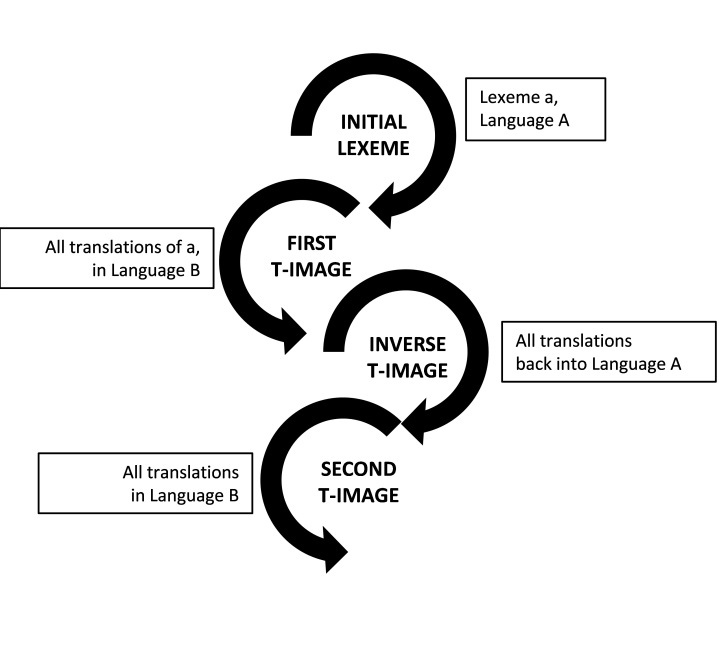
\includegraphics[height=.3\textheight]{figures/Vandevoorde2-img7.jpg}
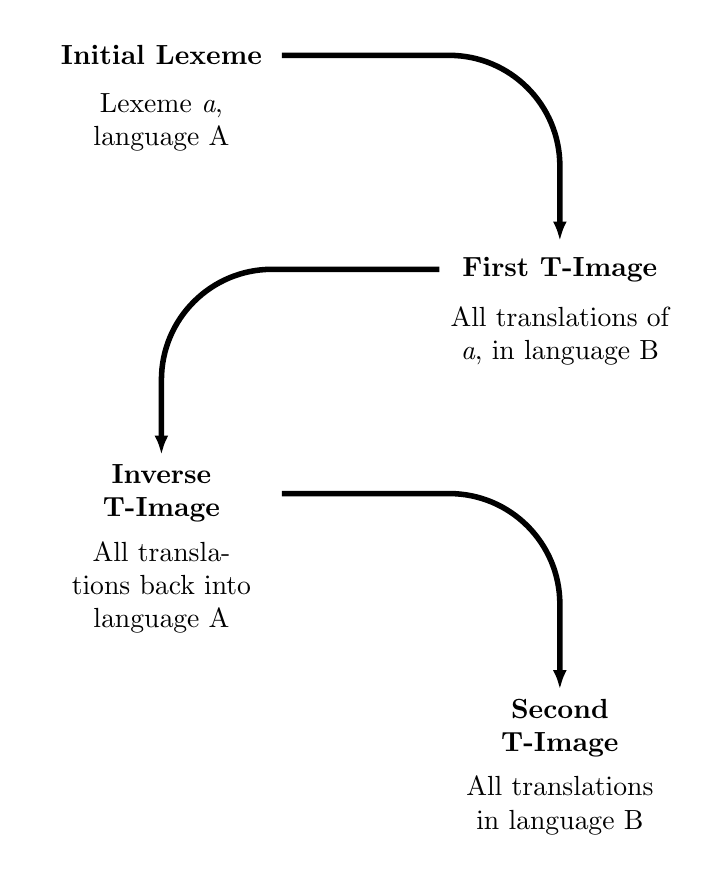
\begin{tikzpicture}
\usetikzlibrary{arrows.meta,positioning,decorations.markings} 
\tikzset{
    box/.style={
           rectangle,
           text width=8em,
           minimum height=2em,
           text centered,
           font=\bfseries},
    explanation/.style={
           rectangle,
           text width=9em,
           minimum height=2em,
           text centered},
    % Define arrow style
    arrow/.style= {
           ->,
           -{Latex[length=7pt,width=5pt]},
           line width=2pt,
           rounded corners=40pt
    }
}
\node[box] (initial) {Initial Lexeme};
\node[box,below right =2cm and 2cm of initial] (first) {First T-Image};
\node[box,below left =2cm and 2cm of first] (inverse) {Inverse T-Image};
\node[box,below right =2cm and 2cm of inverse] (second) {Second T-Image};
\node[explanation,below = 0cm of initial] (exinitial) {Lexeme \textit{a}, language A};
\node[explanation,below = 0cm of first] (exfirst) {All translations of \textit{a}, in language B};
\node[explanation,below = 0cm of inverse] (exinverse) {All translations back into language A};
\node[explanation,below = 0cm of second] (exsecond) {All translations in language B};
\draw[arrow](initial.east) -| (first.north);
\draw[arrow](first.west) -|  (inverse.north);
\draw[arrow](inverse.east) -| (second.north);
\end{tikzpicture}
\caption{\label{fig:3:8}Work flow of the SMM}
\end{figure}

\subsection{Prerequisites and assumptions}
\label{sec:3.4.2}
A practical prerequisite to carry out the technique is that the researcher needs to have access to a parallel corpus which is preferably at least sentence-aligned. If the corpus is word-aligned, the researcher can work in the most optimal circumstances (but word-alignment can be carried out manually or (semi-)automatically on the parallel sentences under investigation).

From the corpus which has been chosen, the researcher needs to be able to extract a set of alternative translations for each lemma one wishes to investigate \citep[31]{langemets_translations_2005}. After the application of the different steps of the SMM, this will ultimately create a “network of translational correspondences uniting the vocabularies of the two languages” (\citeyear[31]{langemets_translations_2005}). Based on Dyvik’s ideas, and based on the following assumptions (verbatim from \citealt[31--32]{langemets_translations_2005}) “each language [will be used] as the ``semantic mirror'' of the other”. The assumptions \citet[31--32]{langemets_translations_2005} puts forward are as follows:

\begin{enumerate}
\item
Semantically closely related words tend to have strongly overlapping sets of translations.
\item
Words with wide meanings tend to have a higher number of translations than words with narrow meanings.
\item
If a word \textit{a} is a hyponym of a word \textit{b} (such as \textit{tasty} of \textit{good}, for example), then the possible translations of \textit{a} will probably be a subset of the possible translations of \textit{b.}
\item
Contrastive ambiguity, i.e., ambiguity between two unrelated senses of a word, such as the two senses of the English noun \textit{band} (‘orchestra’ and ‘piece of tape’), tends to be a historically accidental and idiosyncratic property of individual words. Hence we don’t expect to find instances of the same contrastive ambiguity replicated by other words in the language or by words in the other languages. (More precisely, we should talk about ambiguous \textit{phonological/graphic} words here, since such ambiguity is normally analysed as homonymy and hence as involving two lemmas.)
\item
Words with unrelated meanings will not share translations into another language, except in cases where the shared (graphic\slash phonological) word is contrastively ambiguous between two unrelated meanings. By assumption (4) there should then be at most one such shared word.
\end{enumerate}


\subsection{Overlap}
\label{sec:3.4.3}
When the SMM is applied to an initial lexeme, three types of word sense relationships can arise: “related word senses”, “unrelated word senses” and “mutually unrelated word senses” \citep[32]{langemets_translations_2005}. The first step that needs to be taken is to isolate the mutually unrelated senses of each word (\citeyear[32]{langemets_translations_2005}) for which the resulting lexemes of the first T-image are used. I will illustrate the difference between related word senses, unrelated word senses and mutually unrelated word senses with the example of the Dutch word \textit{bank} (\figref{fig:3:9}), which can be translated in French as \textit{institution financière} (`financial institution'), \textit{banque} (`financial institution'), \textit{banc} (`seat') and \textit{fauteuil} (`armchair'). This distinction between the different types of senses presented in the following sub-sections is based on Dyvik’s procedure for word sense isolation.

\begin{figure}\scriptsize
% 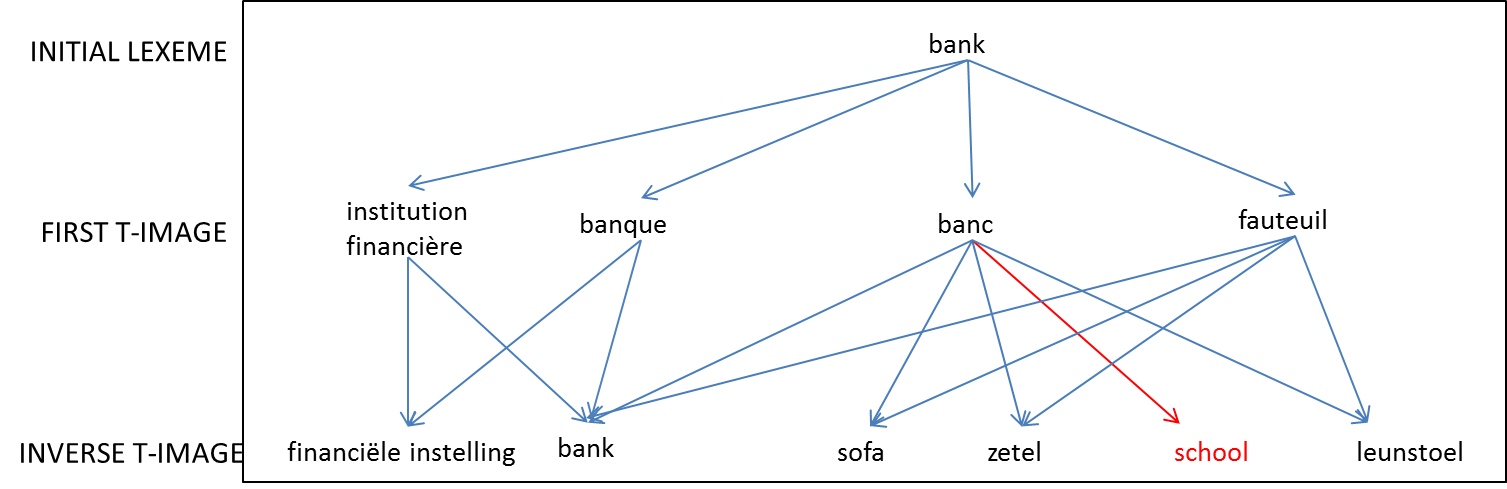
\includegraphics[height=.3\textheight]{figures/Vandevoorde2-img8.png} 
\begin{tikzpicture}
    \matrix (SMM) [draw,matrix of nodes,nodes in empty cells,row 3 column 5/.style=red,row sep=1cm,column sep=2em] {
        \phantom{institution financière} & & bank & & & \\
        institution financière & banque & & banc & & fauteuil\\
        financiële instelling & bank & sofa & zetel & [color=red]school & leunstoel\\
    };
    \foreach \i in {1,2,4,6} \draw[->] (SMM-1-3.south) -- (SMM-2-\i);
    \path[->] (SMM-2-1.south) edge (SMM-3-1)
                              edge (SMM-3-2);
    \path[->] (SMM-2-2.south) edge (SMM-3-1)
                              edge (SMM-3-2);                              
    \path[->] (SMM-2-4.south) edge (SMM-3-2)
                              edge (SMM-3-3)
                              edge (SMM-3-4)
                              edge [color=red] (SMM-3-5)
                              edge (SMM-3-6);
    \path[->] (SMM-2-6.south) edge (SMM-3-2)
                              edge (SMM-3-3)
                              edge (SMM-3-4)
                              edge (SMM-3-6);
    \node[left=.5cm of SMM-1-1.west,align=left] {\scshape initial\\lexeme};
    \node[left=.5cm of SMM-2-1.west,align=left] {\scshape first\\t-image};
    \node[left=.5cm of SMM-3-1.west,align=left] {\scshape inverse\\t-image};
\end{tikzpicture}
\caption{\label{fig:3:9}Example of the (ficticious) SMM of \textit{bank}}
\end{figure}

\subsubsection{Unrelated word senses}
\label{sec:3.4.3.1}
The set of translations back into Dutch (the inverse T-image) of \textit{banque} and \textit{banc} only share the initial lexeme \textit{bank} itself in the inverse T-image. \textit{Banque} (\figref{fig:3:10}) is connected in the inverse T-image to (i.e. can be translated back into Dutch as) \textit{bank} and \textit{financiële} \textit{instelling.} As a consequence, it could be stated that the inverse T-image\textit{s} \textit{bank} and \textit{financiële} \textit{instelling} are semantically related to each other (via \textit{banque}):

\begin{figure}
% 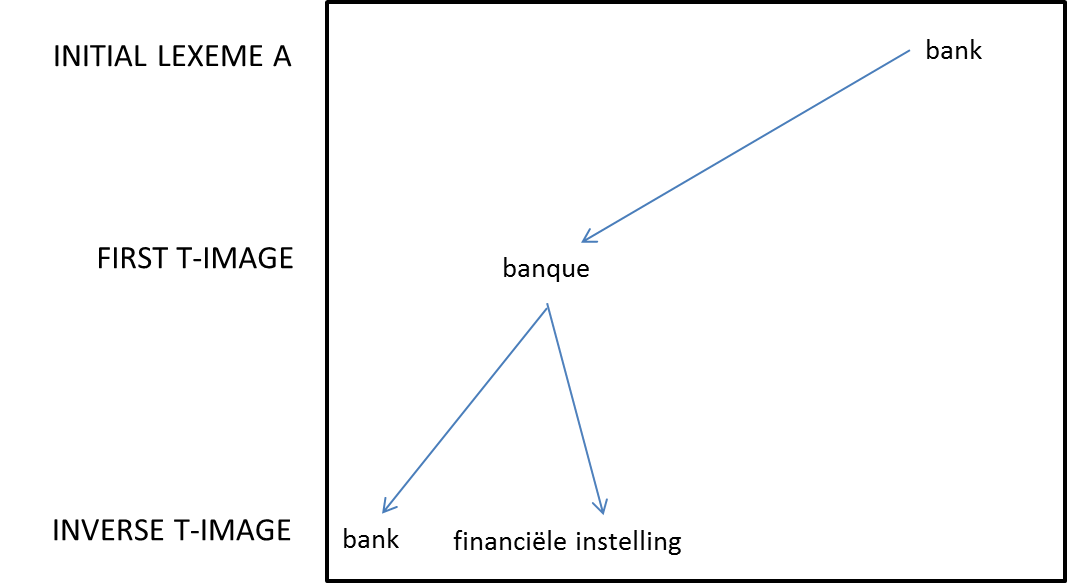
\includegraphics[height=.3\textheight]{figures/Vandevoorde2-img9.png}
\begin{tikzpicture}
    \matrix (SMM) [draw,matrix of nodes,nodes in empty cells,row sep=1cm,column sep=2em] {
        & & bank\\
        & banque &\\
        bank & financiële instelling &\\
    };
    \draw[->] (SMM-1-3) -- (SMM-2-2);
    \draw[->] (SMM-2-2) -- (SMM-3-1);
    \draw[->] (SMM-2-2) -- (SMM-3-2);
    \node[left=1cm of SMM-1-1.center,] {\scshape initial lexeme a};
    \node[left=1cm of SMM-2-1.center,] {\scshape first t-image};
    \node[left=1cm of SMM-3-1.center,] {\scshape inverse t-image};
\end{tikzpicture}
\caption{\label{fig:3:10}{Inverse} {T-image} {of} {banque}}
\end{figure}

\textit{Banc} (\figref{fig:3:11}) on the other hand, is connected in the inverse T-image to \textit{bank,} \textit{sofa,} \textit{zetel} and \textit{leunstoel,} which means that the inverse T-image lexeme \textit{bank} is semantically related to the other inverse T-image lexemes \textit{sofa,} \textit{zetel} and \textit{leunstoel} (via \textit{banc}):

\begin{figure}
% 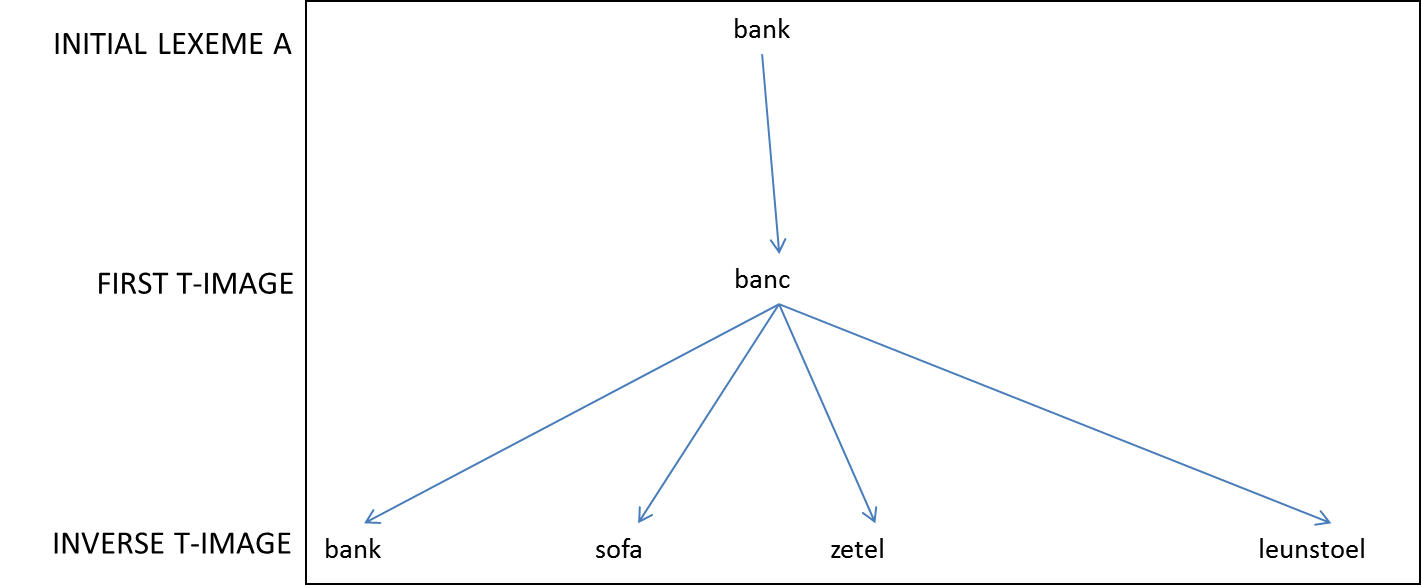
\includegraphics[height=.3\textheight]{figures/Vandevoorde2-img10.png}
\begin{tikzpicture}
    \matrix (SMM) [draw,matrix of nodes,nodes in empty cells,row sep=1cm,column sep=2em] {
        & bank & &\\
        & banc & &\\
        bank & sofa & zetel & leunstoel\\
    };
    \draw[->] (SMM-1-2) -- (SMM-2-2);
    \foreach \i in {1,2,3,4} \draw[->] (SMM-2-2) -- (SMM-3-\i);
    \node[left=1cm of SMM-1-1.center,] {\scshape initial lexeme a};
    \node[left=1cm of SMM-2-1.center,] {\scshape first t-image};
    \node[left=1cm of SMM-3-1.center,] {\scshape inverse t-image};
\end{tikzpicture}
\caption{\label{fig:3:11}Inverse T-image of \textit{banc}}
\end{figure}

The first T-images \textit{banque} and \textit{banc} only share \textit{bank} on the level of the inverse T-image, so \textit{banque} and \textit{banc} are “not directly connected by means of intersections with other sets” \citep[32]{langemets_translations_2005} indicating that their semantic relatedness cannot be proven (and that Dutch \textit{bank} is contrastively ambiguous between French \textit{banque} (`financial institution') and \textit{banc} (`seat')). This observation corresponds with Dyvik’s assumption (4) \citep[31--32]{langemets_translations_2005}: the Dutch lexeme \textit{bank} is indeed \textit{homonymous} between \textit{bank} (`financial institution') and \textit{bank} (`seat'). There is also evidence here for Dyvik’s assumption (5) \citep[31--32]{langemets_translations_2005}: the words \textit{banque} and \textit{banc} indeed only share (“at most”) one word (translation) at the level of the inverse T-image, i.e. the contrastively ambiguous \textit{bank.} Hence, an initial lexeme (e.g. \textit{bank}) possesses two distinct, unrelated senses (e.g. `financial institution' and `seat') if the only shared word between their two sets of lexemes in the inverse T-image is the initial lexeme (which is the case here: the two sets only share \textit{bank}).

\subsubsection{Related word senses}
\label{sec:3.4.3.2}
Looking at the first T-images \textit{banc} and \textit{fauteuil} (Figures \ref{fig:3:11} and \ref{fig:3:13}), we see that \textit{banc} is connected to \textit{bank,} \textit{sofa,} \textit{zetel} and \textit{leunstoel} in the inverse T-image (\figref{fig:3:9}), and that \textit{fauteuil} is connected to \textit{bank,} \textit{sofa,} \textit{zetel} and \textit{leunstoel} in the inverse T-image (\figref{fig:3:13}). In their inverse T-images, \textit{banc} and \textit{fauteuil} share, apart from \textit{bank}, also \textit{sofa,} \textit{zetel} and \textit{leunstoel}. \textit{Banc} and \textit{fauteuil} are thus directly connected by means of intersections with other sets: they do not only share \textit{bank} in the inverse T-image, they also share \textit{sofa,} \textit{zetel} and \textit{leunstoel}, proving the closer semantic relatedness of \textit{banc} and \textit{fauteuil}, and also showing that \textit{bank,} \textit{sofa,} \textit{zetel} and \textit{leunstoel} are semantically related.

\begin{figure}
% 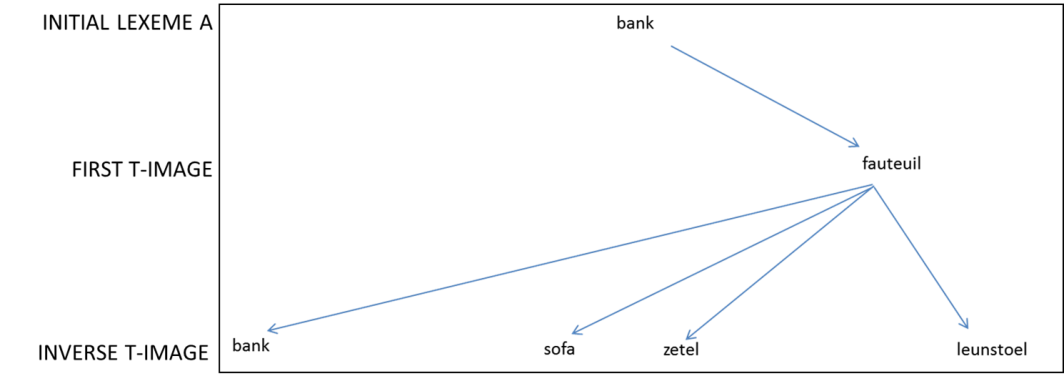
\includegraphics[height=.3\textheight]{figures/Vandevoorde2-img12.png}
\begin{tikzpicture}
    \matrix (SMM) [draw,matrix of nodes,nodes in empty cells,row sep=1cm,column sep=2em] {
        & bank & &\\
        &  & & fauteuil\\
        bank & sofa & zetel & leunstoel\\
    };
    \draw[->] (SMM-1-2) -- (SMM-2-4);
    \foreach \i in {1,2,3,4} \draw[->] (SMM-2-4) -- (SMM-3-\i);
    \node[left=1cm of SMM-1-1.center,] {\scshape initial lexeme a};
    \node[left=1cm of SMM-2-1.center,] {\scshape first t-image};
    \node[left=1cm of SMM-3-1.center,] {\scshape inverse t-image};
\end{tikzpicture}
\caption{\label{fig:3:13}Inverse T-image of \textit{fauteuil}}
\end{figure}

\subsubsection{Mutually unrelated word senses}
\label{sec:3.4.3.3}
A final possible scenario concerns the example of the Dutch word \textit{school} (`school') in the inverse T-image (look back at \figref{fig:3:9}, the example of the (fictitious) SMM of \textit{bank).} Dutch \textit{school} (`school') is a possible translation back into Dutch of the French first T-image word \textit{banc}, in its meaning `school of fishes'. But this latter meaning `school' is not a meaning of Dutch \textit{bank}. Without any knowledge of Dutch and French, the unrelatedness can be deduced from the translational relation: \textit{school} is only translationally related to its French source lexeme \textit{banc}, but it is not related to \textit{bank} on the level of the inverse T-image, implying that the senses of \textit{bank} and \textit{school} are mutually unrelated (\figref{fig:3:14}). Whereas unrelated senses shared only their initial lexeme in the inverse T-image -- enabling a distinction between unrelated senses of the initial lexeme \textit{bank} -- mutually unrelated senses such as \textit{school} and \textit{bank} are not at all related to each other in the inverse T-image.

\begin{figure}
% 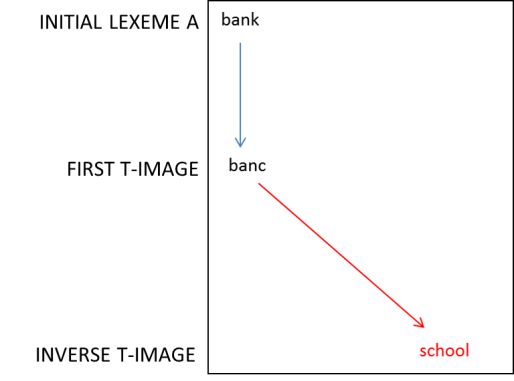
\includegraphics[height=.3\textheight]{figures/Vandevoorde2-img13.png}
\begin{tikzpicture}
    \matrix (SMM) [draw,matrix of nodes,nodes in empty cells,row sep=1cm,column sep=2em,row 3 column 2/.style={red}] {
         bank &\\
         banc &\\
         & school\\
    };
    \draw[->] (SMM-1-1) -- (SMM-2-1);
    \draw[->,color=red] (SMM-2-1) -- (SMM-3-2);
    \node[left=1cm of SMM-1-1.center,] {\scshape initial lexeme a};
    \node[left=1cm of SMM-2-1.center,] {\scshape first t-image};
    \node[left=1cm of SMM-3-1.center,] {\scshape inverse t-image};
\end{tikzpicture}
\caption{\label{fig:3:14}  Mutually unrelated sense \textit{school}}
\end{figure}

\subsubsection{Word sense individuation}
\label{sec:3.4.3.4}
The individuation of word senses can now take place: one of the meanings of \textit{bank} (`financial institution') can be expressed by \textit{bank} and \textit{financiële} \textit{instelling}, another meaning of \textit{bank} (`seat') can be expressed by \textit{bank}, \textit{sofa}, \textit{zetel}, and \textit{leunstoel}. \textit{School} is not a sense of the initial lexeme \textit{bank} and should be disregarded for the further investigation of the senses of \textit{bank.} Dyvik summarizes the principle on which the isolation of word senses takes place as follows:

\begin{quote}
In our translational approach, the semantic fields are isolated on the basis of \textit{overlapping} \textit{t-images} [first T-images]: two senses belong to the same semantic field if they have intersecting first t-images (after sense individuation one member in the intersection is sufficient), or if there is a sequence of such intersecting t-images [first T-images] joining them.\\(\citealt[33]{langemets_translations_2005}, my emphasis, my own terminology is added between brackets for clarity’s sake)
\end{quote}

If one is interested in studying one specific semantic field, a criterion of overlapping (first) t-images or overlap can be observed, meaning that a lexeme at the level of the inverse T-image is only selected when it is related to at least two lexemes on the level of the first T-image. In this way, for the example of \textit{bank,} we see that \textit{school} is linked to only one lexeme on the level of the first T-image viz. \textit{banc}. \textit{School} does not meet the overlap criterion, which is an indication that it pertains to a different semantic field. As for \textit{sofa,} for example, we see that it is linked to both \textit{banc} and \textit{fauteuil} on the level of the first T-image, proving that it pertains to the semantic field under scrutiny.

By consequence, by taking into account a criterion of overlap between the inverse T-image lexemes and the first T-image lexemes (every lexeme selected on the level of the inverse T-image must be a translation of at least two first T-image lexemes), it is guaranteed that mutually unrelated senses are excluded. If words without overlap were included in the analysis (i.e. words which are not related to at least two lexemes on the level of the first T-image), the result of the SMM would risk to contain senses which are mutually unrelated, meaning that they are in fact not a sense of the word under study.

\subsubsection{Necessity of overlap}
\label{sec:3.4.3.5}
The previous paragraphs have shown that overlap is a crucial notion for the selection of those lexemes which pertain to the same semantic field. It has also been shown that the existence of more than one translation for a given word is not a sufficient argument to accept that the word is ambiguous \citep[30]{langemets_translations_2005}. In fact, it only implies that the denotation of the word spans the denotations of two words in a different language \citep[29]{langemets_translations_2005}. This observation has important implications for the use of the translational relation for meaning investigation: “non-transitive translational connections may tie together semantically distant words in the same semantic field” (\citealt[29]{langemets_translations_2005}) – as we have shown in the example of \textit{school}. \citet[29]{langemets_translations_2005} makes an important point about the use of back-translation in this regard: the translational relation should be used with care when it is applied to establish semantic relatedness, and overlap is a necessary criterion if one wants to ``confine'' a semantic field. This problem has also been observed in computational linguistics, where it is generally solved by the addition of another language \citep{gelbukh_five_2013}. The appearance of overlapping translations was already formulated by Ivir\ia{Ivir, Vladimir@Ivir, Vladimir} (see \sectref{sec:2.3.2} of this study: “each L\textsubscript{2} correspondent will be related to a number of other L\textsubscript{1} items too, besides the L\textsubscript{1} with which the analysis was initiated”) but Ivir did, to my knowledge, never exploit this idea explicitly as a validation of the semantic relatedness between the lexemes of a semantic field. Dyvik’s point about the semantic informativity of translations makes his technique directly applicable for lexical semantic research. His reflection about what happens to both ambiguous and unrelated senses when the translational relation is used via back-translation furthermore offers useful insights into what exactly happens when one utilizes translation for meaning-informative tasks.

\section{Extended Semantic Mirrors Method: SMM++}
\label{sec:3.5}
The goal of this methodological chapter is to find an adequate way to retrieve lexemes as candidate-members of a semantic field under scrutiny for both non-translated (original\slash source) language and translated (target) language and to arrive at comparable visualizations of semantic fields of a same initial lexeme in both translated and non-translated language. The SMM developed by \citet{johansson_translational_1998,langemets_translations_2005} and some of the additions proposed by contrastive linguists who applied the technique answer the retrieval question: by going back and forth between sources and translations, and by creating new sets of data at every stage of the exercise, a set of candidate-lexemes of a semantic field can be obtained. The SMM is an expansive, meaning informative technique which can be used for the retrieval of lexemes pertaining to a semantic field.

In order to provide a ``complete'' methodological answer, the SMM will still need to undergo a few extensions. The SMM can indeed help to retrieve candidate-lexemes for a semantic field, but in order to implement Dyvik’s technique as a methodological tool to investigate translational phenomena – via a comparison of semantic fields of translated and non-translated language – a number of issues need to be dealt with.

In this section, I will propose two extensions of the SMM.\footnote{The two extensions to the SMM in \sectref{sec:3.5.1} and \sectref{sec:3.5.2} were first introduced and described in a less elaborate way in \citet{VandevoordeEtAl2017}, an article which is under copyright. Its publisher should be contacted for permission to re-use or reprint the material in any form.} The first extension is concerned with the integration of translation direction and the asymmetry of translation into the retrieval task (\sectref{sec:3.5.1}); the second extension will focus on how the output of the retrieval task can be used as an input for a statistical visualization of a semantic field (\sectref{sec:3.5.2}).

\subsection{Extension 1: Translation direction and asymmetry of translation}
\label{sec:3.5.1}
In the SMM, the translational relation is considered as symmetric, i.e. a relation which exists irrespective of the translation direction. The second T-image results in a set of Language B lexemes which are translations into Language B of the Language A lexemes from the inverse T-image. The second T-image provides the necessary information to establish a semantic field in Language B, just as the resultant information from the inverse T-image (translations into Language A of the Language B lexemes from the first T-image) permits the establishment of a semantic field in Language A, and “paired semantic fields in the two languages involved” \citep[33]{langemets_translations_2005} are created.

For the translation studies scholar, accepting the symmetry of the translational relation would be refuting almost all of the existing research tradition in translation studies. When integrating the SMM for research in TS, one inevitably has to take into account the asymmetric nature of the translational relation as well as the reality of translation direction. This implies that, in my view, translation – as an activity which forms the subject of research in TS – always happens in the direction from a source language into a target language. Differentiating between source and target language does matter in TS, for it is precisely the influence of either source or target language (or both) on the process and the final product of translation which is a pending subject of research in TS.

Two sets of data are therefore created which can form the basis for a comparison of a semantic field of a lexeme under scrutiny: one data set representing non-translated (original\slash source) language (in this case non-translated Dutch), and a second data set representing translated (target) language (in this case translated Dutch with English or French as a source language).

Non-translated Dutch and translated Dutch need to be represented by separate sets of data which furthermore need to be (easily) comparable. In addition to that, the semantic fields created on the basis of these data sets need to consist of lexemes in the same language as the initial lexeme (Dutch). \tabref{tab:3:1} shows the original structure of the SMM as it was conceived by Dyvik. In the fourth column, translation direction is added. Suppose an SMM is carried out on an initial lexeme \textit{a} in language A, for which language A is Dutch and language B is English, then the following scheme applies:

\begin{table}
\caption{\label{tab:3:1} Source and target language in the different steps of the SMM}
%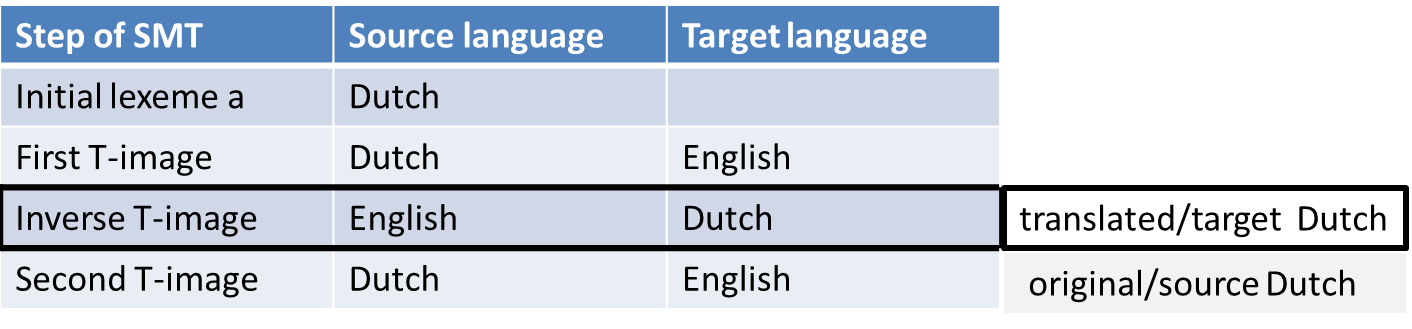
\includegraphics[width=\textwidth]{figures/Vandevoorde2-img14.png}

\fittable{
\begin{tabular}{llll}
\lsptoprule
 Step of SMT & Source language & Target language & Yielded data set \\
 \midrule
 Initial lexeme \textit{a} & Dutch \\
 First T-image & Dutch & English \\
 Inverse T-image & English & Dutch & translated/target Dutch \\
 Second T-image & Dutch & English & original/source Dutch \\
 \lspbottomrule
\end{tabular}
}
\end{table}
  
From \tabref{tab:3:1}, it becomes clear that Dutch (Language A) is a source language in the first and the second T-image and a target language in the inverse T-image. This implies that the data sets which are yielded by the different steps of the SMM are different in translational nature: the data set retrieved at the level of the inverse T-image can be used to analyze translated (target) Dutch, whereas the data set retrieved at the level of the second T-image can be utilized to analyze non-translated (original\slash source) Dutch.

The first extension thus consists in a differentiation between sets of retrieved data within the different steps of the SMM based on their translational status (source or target language). Instead of using the second T-image to make a contrastive comparison (like Dyvik) or disregarding it (like \citealt{aijmer_model_2004}), I assign a new role to this step of the SMM, based on the translational status of the data. This is a necessary first step to make the data obtained via the SMM usable for TS research. Further references in this book to translated language will be written as TransLanguage\textsubscript{A} (in this study TransDutch\textsubscript{ENG} and TransDutch\textsubscript{FR}); referring to the sets of data obtained in the inverse T-image with a Language B (in our study English or French) as a source language and any Language A (in our study Dutch) as a target language. References to non-translated (original\slash source) language will be written as SourceLanguage\textsubscript{A} (in this study SourceDutch); the underlying data set will be the one obtained in the second T-image with any Language A (in this study Dutch) as a source language and any Language B (here: English or French) as a target language.

\subsection{Extension 2: Statistical implementability of the data sets}
\label{sec:3.5.2}
In the previous section, I dealt with the asymmetric nature of translation and determined a way to compile sets of translated and non-translated language by extending the existing SMM. The next step is to arrive at comparable visualizations of those sets of lexemes. The information which has so far been obtained only gives the researcher sets of lexemes but does not propose any kind of organization of those lexemes which could give further information about the semantic relatedness between the lexemes.

Within the original SMM, hierarchical patterns are “only based on overlap relations among \textit{t-}images” and are obtained by ranking the lexemes “independently of frequency of occurrence” \citep[73]{johansson_translational_1998}. The degree of semantic similarity between the lexemes in the created hierarchy is only based on the number of overlapping translations while frequency information is excluded. \tabref{tab:3:2} shows a fictitious example of the translational relation in the inverse T-image of Dutch \textit{bank} with French as a pivot language. Based on this information, and following Dyvik, the centrality of \textit{bank} in a field with \textit{bank,} \textit{financiële} \textit{instelling,} \textit{sofa} and \textit{leunstoel} could be deduced from the fact that \textit{bank} is a translation of all three French lexemes \textit{banque,} \textit{banc} and \textit{fauteuil}.

A visualization based solely on overlapping t-images is usually realized via Venn diagrams \citep{dyvik_semantic_2011}, which tend to get rather complex to interpret. This apparent weak point of the SMM has led computational linguists to propose different methods of visualization which can be of use for computational research purposes (see e.g. \citealt{ganter_conceptual_2005}). It is not in the scope of this book to computationally implement the SMM. However, the objective to create visualizations which can provide more insights into the alleged semantic differences between translated and non-translated language on the basis of the SMM implies the use of methods more closely connected to distributional semantics. Within that framework, the typical approach is to collect occurrence counts of words and other words\slash features in a frequency table. The reason is that frequencies indicate the strength of certain relations, i.e. they will tell us which patterns are important. Such frequency tables can be thought to represent translated language when the translated lexemes are represented as rows with their source language lexemes as column variables. They can represent non-translated language when the non-translated (source language) lexemes are represented as rows with their translations as column variables. The integration of frequency information is the second major extension to the SMM. If frequency information is now integrated into the previously given fictitious example of \textit{bank}, the result looks for non-translated (original\slash source) language \textit{bank} are in \tabref{tab:3:3} and for translated (target) language \textit{bank} in \tabref{tab:3:4}.

\begin{table}\caption{Overlapping translations of \textit{bank} (ficticious) in the inverse T-image\label{tab:3:2}}
\begin{tabularx}{\textwidth}{Qcccc}
\lsptoprule
%%[Warning: Draw object ignored]
{is} {translated} {as} & {bank\textsubscript{[nl]}} & {financiële} {instelling\textsubscript{[nl]}} & {sofa\textsubscript{[nl]}} & {leunstoel\textsubscript{[nl]}}\\\midrule
{banque\textsubscript{[fr]}} & \Checkmark & \Checkmark & \XSolidBrush & \XSolidBrush\\
{banc\textsubscript{[fr]}} & \Checkmark & \XSolidBrush & \Checkmark & \Checkmark\\
{fauteuil\textsubscript{[fr]}} & \Checkmark & \XSolidBrush & \Checkmark & \Checkmark\\
\lspbottomrule
\end{tabularx}
\end{table}

\begin{table}
\caption{Frequency table for original \textit{bank} – second T-image (fictitious)\label{tab:3:3}}
\begin{tabularx}{\textwidth}{Xrrr}
\lsptoprule
{is} {translated} {n} {times} {as} & {banque\textsubscript{[fr]}} & {banc\textsubscript{[fr]}} & {fauteuil\textsubscript{[fr]}}\\\midrule
{bank\textsubscript{[nl]}} & 231 & 61 & 45\\
{financiële} {instelling\textsubscript{[nl]}} & 178 & 0 & 0\\
{sofa\textsubscript{[nl]}} & 0 & 124 & 32\\
{leunstoel\textsubscript{[nl]}} & 0 & 27 & 76\\
\lspbottomrule
\end{tabularx}
\end{table}

\begin{table}
\caption{Frequency table for translated \textit{bank} -- \textit{inverse} \textit{T-image} (fictitious)\label{tab:3:4}}
\begin{tabularx}{\textwidth}{Xrrr}
\lsptoprule
{is} {n} {times} a translation of & {banque\textsubscript{[fr]}} & {banc\textsubscript{[fr]}} & {fauteuil\textsubscript{[fr]}}\\\midrule
{bank\textsubscript{[nl]}} & 230 & 32 & 45\\
{financiële} {instelling\textsubscript{[nl]}} & 121 & 0 & 0\\
{sofa\textsubscript{[nl]}} & 0 & 98 & 32\\
{leunstoel\textsubscript{[nl]}} & 0 & 67 & 43\\
\lspbottomrule
\end{tabularx}
\end{table}

The occurrence counts in the frequency tables implicitly also contain the number of overlapping translations (or source language lexemes). Hence, the frequency tables contain information about both the frequency of co-occurrence of each source language lexeme (or translation) with each translation (or source language lexeme) as well as overlap information about which translations (or source language lexemes) are attested for each source language lexeme (or translation). Advanced statistical techniques can now be applied upon the data sets, opening the way to statistical visualization techniques such as Correspondence Analysis \citep{greenacre_correspondence_2007,lebart_exploring_1998} and Hierarchical Cluster Analysis (\citealp[138]{baayen_analyzing_2008}; \citealp[336]{gries_statistics_2013}), a technique that will allow for a visual representation of the similarities and differences between the sets of lexemes. Previous research in contrastive linguistics has shown that Hierarchical Cluster Analysis is an excellent tool for the evaluation of corpus-based, lexico-semantic analyses \citep{evans_behavioral_2009,libben_behavioral_2012,glynn_cluster_2014}.


\subsection{Technical fine-tuning}
\label{sec:3.5.3}
Although the integration of frequency information into the SMM makes it possible to process the results statistically, one problem still remains. SMM is an expansive technique, implying that with every step more and new information is generated, in this case: new translation solutions for the lexeme(s) are retrieved, and their number increases in every step of the mirror analysis. Although this effect is of course at the core of the technique, it also implies that the number of possible translation solutions grows exponentially with every step of the mirror analysis, leading to data sets which are difficult if not impossible (i) to manage manually or even semi-automatically and (ii) to compare with each other (depending on the initial lexeme in Language A one chooses or on the Language B one chooses, the SMM will select different lexemes).

First, let us take a closer look at the problem of how to manage these (ever) expanding data sets within the retrieval task of the SMM. Translators come up with very creative solutions, even in non-fictional, non-literary texts. For example, within a corpus study this creativity results in the following: for a verb as ``basic'' as \textit{beginnen} `to begin', more than 47 different translations in English appear for a total of 382 translational pairs of sentences with \textit{beginnen} in the Dutch source text in the Dutch Parallel Corpus. It can be very interesting, both from a contrastive linguistic as from a translational perspective, to investigate all these instances, but it would not answer one of the main research questions of this book: how to compare semantic relationships in translated language and non-translated language. For this reason, I agree with Dyvik to exclude completely unpredictable translations – translators’ idiosyncracies – from our analysis. More specifically, I will apply a frequency threshold of three attestations for every translation, allowing me to work with a manageable number of possible translational pairs. This choice is motivated by pragmatic considerations. Firstly, a frequency threshold below three attestations generates additional manual annotation work, endangering the feasibility of the task. Solutions such as automatic word alignment with GIZA++ did not yield satisfying results due to insufficient corpus size, and word aligned parallel corpora are not available for the language pairs in this book. Secondly, with respect to the statistical processing of the data, \citet[133]{evert_statistics_2004} argues against the inclusion of hapax and dis legomena, providing an additional argument in favor of a frequency threshold of three observations:

\begin{quote}
[f]or the time being, however, we must assume that probability estimates and $p$-values for the lowest-frequency types are distorted in unpredictable ways. [...] [T]hese conclusions provide theoretical support for frequency cutoff thresholds. Data with cooccurrence frequency f < 3, i.e. the hapax and dis legomena, should always be excluded from the statistical analysis \citep[133]{evert_statistics_2004}.
\end{quote}

A second restriction of the data is necessary to make sure that the data sets are also acceptably comparable. I will therefore respect the following rule of selection for data at the level of the second T-image (representing non-translated language): in the second T-image, an observation (source-target sentence pair holding the lexeme under investigation) will only be selected when the Language B translation is identical to one of the Language B source language lexemes of the inverse T-image (representing translated language). As a result, the row names and column variables of the data matrices in the inverse T-image (representing translated language) and the second T-image (representing non-translated language) will be identical, their difference will be in their status. In the frequency table representing non-translated language (SourceDutch), the rows are (Dutch) source language lexemes and the columns are (English or French) translations, in the frequency table representing translated language (TransDutch\textsubscript{ENG} or TransDutch\textsubscript{FR}), the rows are (Dutch) translations and the columns are (English or French) source language lexemes. Of course, the frequency counts in the tables will also be different (as illustrated by the difference between \tabref{tab:3:3} and \tabref{tab:3:4} for the fictitious example of \textit{bank}). A similar restriction was also suggested by \citet[60]{johansson_translational_1998} in order to eliminate those results which are unrelated to the initial lexeme. Shortly put: the lexemes which are members of each of the data sets selected for statistical analysis and further visualization are kept identical (the inverse T-image provides the lexemes for the semantic field of translated language, and the second T-image provides the lexemes for the semantic field of non-translated language), but the ``content'' (frequency information and translational status) of the data sets differs since source and target language are in fact inversed in the two sets of data. In this way, we solve \citeauthor{krzeszowski_contrasting_1990}'s semantic paradox which we are facing here that “what is identical is not subject to comparison, and what is different is not comparable” \citep[7]{krzeszowski_contrasting_1990}: we propose to select identical lexemes, but because of their translational status, both data sets are nonetheless different; we thus solve the paradox and make the two sets of data comparable to each other.

In conclusion, the previously mentioned adjustments will lead to (i) a selection of a manageable amount of manually controlled data on which a quantitative analysis can be carried out and (ii) the comparability of the two data sets.

\subsection{Conceptual issue}\label{sec:3.5.4}
The application of the SMM++ leads to the creation of comparable data sets of translated and non-translated language. The frequency tables are obtained on the basis of translational data and following a translation-based method. For the data set of non-translated (source) language, both the nature of the data as well as the nature of the method could well be held against it. In this section, I will show that it can be made conceptually acceptable to use translational data and a translation-based method to obtain a frequency table for non-translated language.

One of the basic assumptions when implementing a method such as the SMM is exactly the idea that the translational relationship can be used as an analytical basis, i.e. to consider “sets of translationally corresponding items across languages as the primitives of semantic descriptions” \citep[31]{langemets_translations_2005}. As a consequence, the translations which are generated by the SMM in the pivot language(s) can be considered as analogous to semantic features. These semantic primitives or semantic features are similar to the attributes of the prototype-based theory of semantic organization we presented in \chapref{sec:2}. Under the assumption that translations can indeed constitute a kind of attribute, a semantic description on the basis of translations becomes acceptable and the visualization of non-translated language on the basis of translations (as semantic features) becomes defensible too. The fact that different languages carve up the world in different ways is used to the advantage of the proposed method: contrastive differences can be seen as a reflection of difference(s) (in classification) of semantic properties and can consequently be semantically informative.

As explained in \sectref{sec:3.5.1}, the corpus observations which are selected to investigate non-translated (source) language are source language data. As a consequence, translation cannot have affected the use of a specific source language lexeme in its non-translated environment simply because it is not translated. The use of source language data to represent non-translated data is, in my opinion, conceptually acceptable, but one should keep in mind that the mere selection of a text as a source text, i.e. a text selected to be translated, does have a certain impact: some texts might be more often and more commonly selected for translation than others, whereas still others may have been excluded due to various factors, sometimes referred to as preliminary norms \citep{toury_descriptive_1995}. In addition, the lexeme selection method is and remains of course based on a translation-based technique, viz. the SMM++. While its translational nature assures the semantic relatedness, the ungraspable trace of the translational basis of the method on the selection of the lexemes needs to be accepted. One could argue that monolingual data would better fit the purpose of visualizing non-translated language structure. Although this is a valid point, previous studies using monolingual reference corpora have faced major comparability issues due to corpus size or uncertainty about the (translational) status of the texts in the presumed original language corpora (e.g. \citealt{musolff_conceptual_2014}). Another option would be to base the visualizations on a different hypothesis which does not rely on translations as semantic features. If, for instance, the distributional hypothesis were applied, then only the monolingual contextual information of the Dutch source language sentences would have to be used for the visualization of non-translated language.\footnote{\citet{vandevoorde_distributional_2016} show that semantic fields of \textit{beginnen}\slash inchoativity obtained via the distributional method are similar to those obtained via the translational method.}

Some additional steps to keep the possible source language influence to a minimum are taken, ensuring a ``fair'' comparison between original language and translated language using the same technique, the same hypothesis and the same data. As a first precautionary measure, I will refer to these data sets and their subsequent visualizations as SourceLanguage\textsubscript{A} instead of OriginalLanguage\textsubscript{A}. Secondly, I will combine the data of two semantic mirrors for the SourceLanguage\textsubscript{A} data set. This means that the semantic features from two distinct languages will be combined for the visualization of SourceLanguage\textsubscript{A}. In this way, I maximize the neutralization of any possible specific influence of the semantic features (translations) on the visualization of SourceLanguage\textsubscript{A}.

\section{Applying the first extension of the SMM to retrieve data sets for beginnen}
\label{sec:3.6}
In this section, the SMM++ retrieval task is applied to obtain data sets which can represent the semantic field of \textit{beginnen}/inchoativity in Dutch. The corpus which was used to retrieve the data is the Dutch Parallel Corpus (see \sectref{sec:3.3}). I will describe how the three resultant data sets were obtained by applying the SMM++ to the initial lexeme \textit{beginnen} in the DPC. One data set is obtained for non-translated Dutch (SourceDutch) and two data sets for translated Dutch, one with English as a Language B (TransDutch\textsubscript{ENG}) and a second one with French as a Language B (TransDutch\textsubscript{FR}). All data sets were retrieved following the exact procedure described above. \textit{Beginnen} was chosen as the initial lexeme, because it can be considered as the most prototypical expression of inchoativity: it is used more frequently than its closest near-synonym \textit{starten} `to start' with 291,438 hits for \textit{beginnen} versus 23,986 for \textit{starten} in the Dutch reference corpus SONAR \citep{spyns_construction_2013}.

The first mirroring will be carried out with English as a Language B, the second mirroring with French as a Language B. The second T-image of \textit{beginnen} with English as a Language B and the second T-image of \textit{beginnen} with French as a Language B will be joined into one data set SourceDutch. The inverse T-image of \textit{beginnen} with English as a Language B will result in the data set TransDutch\textsubscript{ENG}, the inverse T-image of \textit{beginnen} with French as a Language B will result in the data set TransDutch\textsubscript{FR}.

\subsection[First T-images of \textit{beginnen}\textsubscript{ENG} and \textit{beginnen}\textsubscript{FR}]{First T-images of \textit{beginnen}\textsubscript{ENG} and \textit{beginnen}\textsubscript{FR}\protect\footnote{Beginnen\textsubscript{ENG} refers to the semantic mirroring initiated by the initial lexeme \textit{beginnen} and with English as a Language B. Beginnen\textsubscript{FR} refers to the semantic mirroring initiated by the initial lexeme \textit{beginnen} and with French as a Language B.}}\label{sec:3.6.1}

The SMM++ was first carried out with English as a pivot language. Attestations of the Dutch verb \textit{beginnen} were queried in the DPC via the interface developed by \citet[62]{delaere_translations_2015}. A lemma-based query was carried out rendering all sentences with \textit{beginnen} in any of its inflected forms. From the 1,867 resulting observations, 382 fulfilled the criterion of translation direction (Dutch as a source language, English as a target language). Each of the 382 sentences was manually annotated, meaning that the translation of \textit{beginnen} was recorded for every sentence. For the example \REF{ex:3:1} below, \textit{take} \textit{up} was annotated as the translation of \textit{beginnen}:


\ea (dpc-vla-001920-nl, my emphasis)\label{ex:3:1}\\
\textsc{source:} Zo vermeldde iemand bijvoorbeeld: “Ongeveer 80 procent van de afgestudeerden van onze kunstacademie zal een carrière \Highlight{beginnen} in de creatieve industrie".\\\relax
\ob`Someone mentioned for example: “About 80 percent of the graduates of our academy of arts will \Highlight{begin} a career in the creative industry”.'\cb\smallskip\\
{\scshape target:} For example, in one case “Around 80 percent of graduates from our art school will \Highlight{take up} careers in the creative industries". 
\z

From the 382 observations, 46 were disregarded for further analysis. Three reasons for elimination were distinguished. Two of them apply to all data retrieval and annotation tasks in our study, the third one is specific to the case of \textit{beginnen} with English as a Language B.

\begin{enumerate}
\item The sentence alignment is erroneous. In this case, it is technically possible to look up the complete texts from which the aligned sentences were extracted and re-align the sentence correctly. However, I chose to disregard the erroneously aligned sentences out of practical considerations.
\item The source language lexeme under consideration is not translated at all (or no translation equivalent can be indicated in a straightforward way). Observations where the lexeme under study remains untranslated in the target sentence, such as in \REF{ex:3:2}, are disregarded for further analysis:


\ea (dpc-ing-002337-nl, my emphasis)\label{ex:3:2}\\
\textsc{source:} Ondernemers \Highlight{begonnen} koortsachtig op zoek te gaan naar snoeiposten, [...].\\\relax
\ob`Entrepreneurs feverishly \Highlight{began} to look for targets for cut backs'\cb\smallskip\\
\textsc{target:} Company managers feverishly grasped to make savings, [...] 
\z

Although it would as such be interesting to examine why the inchoative aspect disappeared from the target sentence, this question is not addressed in the current study.

\item The third reason to eliminate an observation is when the lexeme \textit{beginnen} is non-lexicalized in translation. This case is particularly relevant to the translation of Dutch \textit{beginnen} into an English progressive structure (although similar translational situations are imaginable for this same verb and surely exist for other verbs, this is the only case encountered within our study of \textit{beginnen} with English and French as languages B). Consider the following example \REF{ex:3:3}:

\ea (dpc-ing-001896-nl, my emphasis)\label{ex:3:3}\\
\textsc{source:} Terwijl de Europese Unie zich stilaan \Highlight{begint} op te maken om 10 nieuwe lidstaten te verwelkomen, blijft de Europese economie een slappe bedoening.\\\relax
\ob`While the European Union \Highlight{begins} gradually to prepare itself to welcome 10 new member states, the European economy reamins a sluggish affair.'\cb\smallskip\\
\textsc{target:} While the European Union \Highlight{is} gradually \Highlight{preparing} to welcome 10 new member states, the European economy remains in the doldrums. 
\z

In this particular example \textit{zich} \textit{opmaken} is translated by \textit{to} \textit{prepare} and \textit{stilaan} is translated by \textit{gradually}. The verb \textit{beginnen} is not translated lexically here; instead its translation is couched in the structure ‘to be+ing-form’ applied to the verb \textit{to} \textit{prepare}. Observations where an inchoative verb is translated by a syntactic structure such as `to be+ing-form' were excluded for further analysis. Although annotation was perfectly possible on the technical side, the inchoative aspect of the structure ‘to be+ing-form’ is often very subtle \citep{smith_parameter_1997} and open for debate, as the following example \REF{ex:3:4} clarifies:

\ea (dpc-arc-002037-en, my emphasis)\label{ex:3:4}\\
\textsc{source:} But thanks to technological advances, plasma techniques \Highlight{are playing} an ever greater role in our daily life: just think of fluorescent tubes and flat screen televisions, for example.\smallskip\\
\textsc{target:} Dankzij de technologische ontwikkeling \Highlight{duiken} steeds meer plasmatoepassingen \Highlight{op} in ons dagelijks leven. Denken we maar aan de tl-lampen of aan het vlakke plasmascherm van televisietoestellen.\\\relax
\ob`Thanks to technological development, more and more plasma applications are popping up in our daily live. Think of striplighting or the flat plasma screen of television sets.'\cb
\z

In example \REF{ex:3:4}, the pattern ‘to be+ing-form’ could arguably be said to carry an inchoative aspect. The Dutch target sentence in fact even provides evidence for the inchoative aspect: the verb \textit{to} \textit{play} is not translated into \textit{spelen}, which would have been a perfectly acceptable translation solution and even the readiest one (\textit{een} \textit{rol} \textit{spelen} `to play a role'). Instead, the translator selected the verb \textit{opduiken} `to pop up, to turn up' which lexicalizes the inchoative aspect of the ‘to be+ing-form’ pattern of the English source sentence. The potential relevance of such an observation is of course indisputable but this example also shows that a whole other approach is needed for the annotation and analysis of this type of verb patterns in the source text with their corresponding items in the target text. The reason is that one should also envisage and annotate the translation of those patterns into still other patterns in the target language. This would increase the complexity of the application of the SMM++ considerably, reducing one of its advantages, i.e. the straightforward annotation of a source language lexical item and its translation (into a lexical item). The omission of observations where a verb pattern is proposed as a translation for the lexeme under study could be seen as a shortcoming of this study; a solution for complex annotations is definitely needed. However, in this first application of the SMM++, I reasonably limited the factors of complexity and disregarded this type of verb patterns. In the case of \textit{beginnen}, this can be done by disregarding translations into ‘to be+ing-form’.
\end{enumerate}

The 336 remaining observations for the first T-image of \textit{beginnen}\textsubscript{ENG} (listed in \tabref{tab:3:5}) consist of 44 different translations. From those 44 lexemes, 35 were observed less than 3 times. In other words, only 9 translations met the frequency threshold of 3 observations. Those 9 translations account for 292 of the total of 336 observations. In \tabref{tab:3:5}, the lexemes in \HightlightsName\ meet the frequency threshold of 3 observations and are selected for further analysis. \tabref{tab:3:6} gives a summary of the first step of the SMM++ retrieval task for \textit{beginnen}\textsubscript{ENG}.

\begin{table}
\caption{First T-image of \textit{beginnen}\textsubscript{ENG} (raw frequencies)\label{tab:3:5}}
\begin{tabular}{lr@{\hspace{5em}}lr} 
\lsptoprule
\multicolumn{4}{c}{beginnen}\\\midrule      
{already} &  1            &             {to} {embark} &  2\\
{as} {from} &  1          &           {to} {emerge} &  1\\
{aspiring} &  1           &            {to} {enter} &  2\\
{beginning} {(adj)} &  2  &   {to} {gain} &  1\\
\Highlight{beginning (n)} &  {3}  &   {to} {go} {ahead} &  1\\
\Highlight{first of all} &  {3} &  {to} {go} {into} &  1\\
{fundamental} &  1        &         {to} {kick} {off} &  1\\
{initial} &  1            &             {to} {launch} &  2\\
{introduction} &  1       &        {to} {let} &  1\\
{nascent} &  2            &             \Highlight{to open} &  {5}\\
{new} &  1                &                 {to} {result} &  1\\
{original} &  1           &            {to} {see} &  1\\
\Highlight{start (n)} &  {7}      &       \Highlight{to set up} &  {3}\\
{start-up} {(n)} &  1     &      \Highlight{to start} &  {171}\\
{to} {adopt} &  1         &          {to} {start} {off} &  2\\
{to} {assume} &  1        &         \Highlight{to start out} &  {6}\\
{to} {be} {rooted} &  1   &    \Highlight{to start up} &  {5}\\
{to} {bear} &  1          &           {to} {take} {up} &  2\\
\Highlight{to begin} &  {89}      &       {to} {talk} &  1\\
{to} {come} &  1          &           {to} {try} &  1\\
{to} {commence} &  2      &       {to} {undertake} &  2\\
{to} {develop} &  1       &        {young} &  1\\ \midrule
\multicolumn{4}{c}{TOTAL: 336}\\
\lspbottomrule
\end{tabular}
\end{table}

\begin{table}
\caption{First T-image of \textit{beginnen}\textsubscript{ENG}\label{tab:3:6}}
\small
\begin{tabularx}{\textwidth}{>{\raggedright}p{.4\textwidth}lXlX}
\lsptoprule
Step of the SMM++ & \multicolumn{4}{l}{First T-Image}\\ \midrule
\rowcolor{lsLightGray} Source language & \multicolumn{4}{l}{Dutch}\\
Target language & \multicolumn{4}{l}{English}\\
\rowcolor{lsLightGray} Total queried observations & \multicolumn{4}{l}{382}\\
Total selected observations after discarding erroneous alignments and non-translated observations &  \multicolumn{4}{l}{336}\\
\rowcolor{lsLightGray} Total different translations & \multicolumn{4}{l}{44}\\
Total selected observations after frequency threshold  & \multicolumn{4}{l}{292}\\
\rowcolor{lsLightGray} Total selected different ranslations after frequency threshold & \multicolumn{4}{l}{9}\\
Source language lexeme(s) & \multicolumn{4}{l}{beginnen}\\
\rowcolor{lsLightGray}Selected target language lexemes & 1. & beginning (n) & 6. & to set up \\
\rowcolor{lsLightGray}& 2. & first of all & 7. & to start \\
\rowcolor{lsLightGray}& 3. & start (n) & 8. & to start out \\
\rowcolor{lsLightGray}& 4. & to begin & 9. & to start up \\
\rowcolor{lsLightGray}& 5. & to open  &&\\
\lspbottomrule
\end{tabularx}
\end{table}

The retrieval task of the SMM++ was also carried out with French as a pivot language. \tabref{tab:3:7} summarizes the information of the first T-image of \textit{beginnen}\textsubscript{FR}.

\begin{table}
\caption{First T-image of \textit{beginnen}\textsubscript{FR}\label{tab:3:7}}
\small
\begin{tabularx}{\textwidth}{p{.4\textwidth}lXlX}
\lsptoprule
Step of the SMM++ & \multicolumn{4}{l}{First T-Image}\\ \midrule
\rowcolor{lsLightGray}Source language & \multicolumn{4}{l}{Dutch}\\
Target language & \multicolumn{4}{l}{French}\\
\rowcolor{lsLightGray}Total queried observations & \multicolumn{4}{l}{472}\\
Total selected observations after discarding erroneous alignments and non-translated observations & \multicolumn{4}{l}{398}\\
\rowcolor{lsLightGray}Total different translations & \multicolumn{4}{l}{75}\\
Total selected observations after frequency threshold & \multicolumn{4}{l}{332}\\
\rowcolor{lsLightGray}Total selected different translations after frequency threshold & \multicolumn{4}{l}{19}\\
Source language lexeme(s) & \multicolumn{4}{l}{beginnen}\\
\rowcolor{lsLightGray}Selected target language lexemes &  1.& à partir de & 11.& entrer \\ 
\rowcolor{lsLightGray}& 2. & commencer & 12.& lancer \\ 
\rowcolor{lsLightGray}& 3. & d'abord & 13.& lancer, se \\
\rowcolor{lsLightGray}& 4. & début & 14.& mettre, se \\  
\rowcolor{lsLightGray}& 5. & débutant (adj) & 15.& ouvrir \\
\rowcolor{lsLightGray}& 6. & débutant (n) & 16.& partir \\ 
\rowcolor{lsLightGray}& 7. & débuter & 17.& prendre cours \\  
\rowcolor{lsLightGray}& 8. & démarrer & 18.& (prendre son départ) \\  
\rowcolor{lsLightGray}& 9. &entamer & 19.& recommencer \\
\rowcolor{lsLightGray}& 10.& entreprendre &&  \\
\lspbottomrule
\end{tabularx}
\end{table}

\subsection{Inverse T-images of \textit{beginnen}\textsubscript{ENG} and \textit{beginnen}\textsubscript{FR}}
\label{sec:3.6.2}
The next step of the SMM++ consists in querying the lexemes from the first T-image as source language lexemes in the DPC. For \textit{beginnen}\textsubscript{ENG}, all English sentences containing each of the 9 lexemes from the first T-image are queried, only those sentences where English is the source language and Dutch the target language are selected. For each observation, the translation back into Dutch of the lexeme is annotated, which leads to the summary in \tabref{tab:3:8}. \tabref{tab:3:9} summarizes the results of the inverse T-image of \textit{beginnen}\textsubscript{FR}.

\begin{table}
\caption{Inverse T-image \textit{beginnen}\textsubscript{ENG}\label{tab:3:8}}
\small
\begin{tabularx}{\textwidth}{p{.4\textwidth}lXlX}
\lsptoprule
Step of the SMM++ & \multicolumn{4}{l}{Inverse T-Image}\\ \midrule
\rowcolor{lsLightGray} Source language & \multicolumn{4}{l}{ English}\\
Target language & \multicolumn{4}{l}{ Dutch}\\
\rowcolor{lsLightGray} Total queried observations & \multicolumn{4}{l}{ 1217}\\
Total selected observations after discarding erroneous alignments and non-translated observations & \multicolumn{4}{l}{ 1029}\\
\rowcolor{lsLightGray} Total different translations & \multicolumn{4}{l}{ 148}\\
Total selected observations after frequency threshold and overlap & \multicolumn{4}{l}{ 829}\\
\rowcolor{lsLightGray} Total selected different translations after frequency threshold and overlap & \multicolumn{4}{l}{ 24}\\
Source language lexeme(s) & 1. & beginning (n) & 5. & to open \\
& 2. & first of all & 6. & to set up \\
& 3. & start (n) & 7. & to start \\
& 4. & to begin & 8. & to start out \\
& 9. & to start up & & \\
\rowcolor{lsLightGray}Selected target language lexemes & 1. &  aanvang & 13.& opening\\
\rowcolor{lsLightGray}& 2. & (allereerst) & 14.& oprichten\\
\rowcolor{lsLightGray}& 3. & begin & 15.& opstarten\\
\rowcolor{lsLightGray}& 4. & \textit{beginnen} & 16.& opzetten\\
\rowcolor{lsLightGray}& 5. & eerst & 17.& sinds\\
\rowcolor{lsLightGray}& 6. & gaan & 18.& start\\
\rowcolor{lsLightGray}& 7. & inzetten & 19.& start-\\
\rowcolor{lsLightGray}& 8. & komen & 20.& starten\\
\rowcolor{lsLightGray}& 9. & krijgen & 21.& steeds meer\\
\rowcolor{lsLightGray}& 10.& maken & 22.& van start gaan\\
\rowcolor{lsLightGray}& 11.& ontstaan & 23.& vanaf\\
\rowcolor{lsLightGray}& 12.& openen & 24.& worden\\
\lspbottomrule
\end{tabularx}
\end{table}

\begin{table}
\caption{Inverse T-image of \textit{beginnen}\textsubscript{FR}\label{tab:3:9}}
\small
\begin{tabularx}{\textwidth}{p{.4\textwidth}lXlX}
\lsptoprule
Step of the SMM++ & \multicolumn{4}{l}{Inverse T-Image}\\ \midrule
\rowcolor{lsLightGray} Source language & \multicolumn{4}{l}{French}\\
Target language & \multicolumn{4}{l}{Dutch}\\
\rowcolor{lsLightGray} Total queried observations & \multicolumn{4}{l}{ 2409}\\
Total selected observations after discarding erroneous alignments and non-translated observations & \multicolumn{4}{l}{ 1706}\\
\rowcolor{lsLightGray} Total different translations & \multicolumn{4}{l}{ 339}\\
Total selected observations after frequency threshold and overlap & \multicolumn{4}{l}{ 1179}\\
\rowcolor{lsLightGray} Total selected different translations after frequency threshold and overlap & \multicolumn{4}{l}{ 39}\\
Source language lexeme(s) & 1.& à partir de & 10.& entreprendre\\
& 2.& commencer & 11.& entrer\\
& 3.& d'abord & 12.& lancer\\
& 4.& début & 13.& lancer, se\\
& 5.& débutant (adj) & 14.& mettre, se\\
& 6.& débutant (n) & 15.& ouvrir\\
& 7.& débuter & 16.& partir\\
& 8.& démarrer & 17.& prendre cours\\
& 9.& entamer & 18.& recommencer \\
\rowcolor{lsLightGray} Selected target language lexemes & 1. & aanvang & 21.& ontstaan\\
\rowcolor{lsLightGray}& 2.& aanvangen & 22.& ontwikkelen\\
\rowcolor{lsLightGray}& 3.& aanvankelijk & 23.& op basis van\\
\rowcolor{lsLightGray}& 4.& aanvatten & 24.& openen\\
\rowcolor{lsLightGray}& 5.& begin & 25.& oprichten\\
\rowcolor{lsLightGray}& 6.& begin- & 26.& opstarten\\
\rowcolor{lsLightGray}& 7.& \textit{beginnen} & 27.& opzetten\\
\rowcolor{lsLightGray}& 8.& belanden & 28.& sinds\\
\rowcolor{lsLightGray}& 9.& doen & 29.& sluiten\\
\rowcolor{lsLightGray}& 10.& een aanvang nemen & 30.& start\\
\rowcolor{lsLightGray}& 11.& eerst & 31.& starten\\
\rowcolor{lsLightGray}& 12.& gaan & 32.& storten, zich\\
\rowcolor{lsLightGray}& 13.& in werking treden & 33.& ten eerste\\
\rowcolor{lsLightGray}& 14.& ingaan & 34.& uitgaan van\\
\rowcolor{lsLightGray}& 15.& komen & 35.& van start gaan\\
\rowcolor{lsLightGray}& 16.& krijgen & 36.& vanaf\\
\rowcolor{lsLightGray}& 17.& lanceren & 37.& vanuit\\
\rowcolor{lsLightGray}& 18.& maken & 38.& vertrekken\\
\rowcolor{lsLightGray}& 19.& nemen & 39.& worden\\
\rowcolor{lsLightGray}& 20.& ondernemen && \\
\lspbottomrule
\end{tabularx}
\end{table}

With regard to the inverse T-image of \textit{beginnen}\textsubscript{FR}, there are two points which require further attention: the first one is the lexeme \textit{prendre} \textit{son} \textit{départ} and the second one relates to the proportion of selected data versus the total of queried data.

The lexeme \textit{prendre} \textit{son} \textit{départ} was initially selected as one of the source language lexemes of the inverse T-image of \textit{beginnen}\textsubscript{FR} (since it met the condition of frequency threshold of 3 observations in the first T-image). However, no observations were found with \textit{prendre} \textit{son} \textit{départ} as a French source language expression. Two explanations are plausible. First, on closer analysis, all observations of the first T-image which rendered \textit{prendre} \textit{son} \textit{départ} as a translation, appeared to stem from two documents (dpc-wst-000014-fr and dpc-wst-000071-fr) which were translated by the same two translators and released by the same text provider. This could suggest that we were dealing with a \mbox{(quasi-)}idiosyncratic expression from the two translators. However, the two documents (dpc-wst-000014-fr and dpc-wst-000071-fr) also share the same subject: they describe walks\slash walk\-ing trails for tourists. This seems in fact to be a typical context in which the expression \textit{prendre} \textit{son} \textit{départ} appears, as the following examples (\ref{ex:3:5} and \ref{ex:3:6}) from the FrWaC\footnote{FrWac is a 1.6 billion word, web-derived corpus \citep{xiao_web_2010} which I consulted here for reference.} corpus confirm:

\ea (corpus position 94673986, my emphasis)\label{ex:3:5}\\
Le parcours vallonné \Highlight{prend son départ} au lotissement de Saint Paul près de la chapelle , traverse le Pont de Reynès et monte au travers de la montagne jusqu' au village .\\\relax
\glt `The hilly path \Highlight{starts from} the townsite of Saint Paul’s near the chapel, crosses the Reynès bridge and goes up across the mountain to the village.' 
\z
\ea (corpus position 269689, my emphasis)\label{ex:3:6}\\
Quant au chemin de fer touristique du Tarn , il \Highlight{prend son départ} à l' ancienne station des Tramways à vapeur du Tarn au centre de Saint-Lieux .\\\relax
\glt `As far as the tourist railway of the Tarn concerns, it \Highlight{starts off} in the old station for steam trams of the Tarn in the centre of Saint-Lieux.'
\z

Other contexts in which \textit{prendre} \textit{son} \textit{départ} can be used are more philosophical in nature, as \REF{ex:3:7} illustrates:

\ea(corpus position 60635066, my emphasis)\label{ex:3:7}\\
Le propos de Laplanche \Highlight{prend son départ} , en effet , de l' idée qu' éros-liaison oeuvre en tant que tel « dans un sens narcissique » , puisqu' il tend , dit -il , à « faire de l' un » ( Lacan ) .\\\relax
\glt `Laplanches comment indeed \Highlight{stems from} the idea that the eros connection is as such as work “in a narcissistic way”, because it tends, so he says, to “the becoming of one” (Lacan).'
\z

These examples show that the lack of observations for \textit{prendre} \textit{son} \textit{départ} as a source language lexeme is not so much due to idiosyncratic language use, but rather to data sparseness in the DPC. Although \textit{prendre} \textit{son} \textit{départ} can be considered as an accepted expression of inchoativity in French, its use is restricted to very specific contexts which the DPC does not provide. As a consequence, further mirroring cannot be carried out for this verbal expression.

A second observation which can be made here is that the final selection of data for \textit{beginnen}\textsubscript{FR} is proportionally smaller than the selection for \textit{beginnen}\textsubscript{ENG} – a little over 70\%, compared to more than 80\% for \textit{beginnen}\textsubscript{ENG}. This is due to a higher ratio of erroneous alignments, but appears to be often the result of an omission in the translation. Translating by omission is one of the strategies indicated by \citet[40]{baker_other_1992}. It is an interesting phenomenon which should not be neglected and from which interesting findings can ensue. In this study, for example, no translation into Dutch could be formally indicated in 59 out of 226 observations for the French adverb \textit{d’abord} (over 26\% of the cases). By contrast, its English equivalent \textit{first} \textit{of} \textit{all} is translated into Dutch in 17 out of 18 observations. Hence, it appears that translators more easily omit French \textit{d’abord} when translating into Dutch than English \textit{first} \textit{of} \textit{all} when translating into the same language. Interestingly, such contrastive comparisons of translation by omission can reveal diverging patterns of translational behavior for different languages and different parts of speech. Unfortunately, observations of translation by omission have to be discarded from this study as zero translations cannot be selected and retrieved as a source language lexeme in the next step of the SMM++.


\subsection{Second T-images of \textit{beginnen}\textsubscript{ENG}\textsubscript{} and \textit{beginnen}\textsubscript{FR}}
\label{sec:3.6.3}
The following step of the SMM++ consists of querying the lexemes from the inverse T-image as Dutch source language lexemes in the DPC. For \textit{beginnen}\textsubscript{ENG}, the translation back into English of each selected observation of one of the 24 source lexemes is annotated. Recall that the data in the second T-image are selected according to an additional restriction, i.e. translations have to be identical to one of the source language lexemes of the inverse T-image. In practice, there are two implications of this additional restriction for the data set \textit{beginnen}\textsubscript{ENG}. First, the total number of selected observations is 17 times smaller than the (enormous) total number of queried observations,\footnote{In order to cope with the vast number of observations, a preliminary statistical word alignment using GIZA++ was carried out. Every statically word-aligned observation was subsequently manually verified. The author wants to thank Els Lefever for her precious help with statistical word alignment.} and second, one source language lexeme \textit{allereerst} had to be discarded because its back-translations into English did not match any of the 9 selected target language lexemes (a problem most probably due to corpus size). These final results of the mirroring are summarized in \tabref{tab:3:10}.\largerpage

\begin{table}[h]
\caption{Second T-image of \textit{beginnen}\textsubscript{ENG}\label{tab:3:10}}
\small
\begin{tabularx}{\textwidth}{p{.4\textwidth}lXlX}
\lsptoprule
Step of the SMM++ & \multicolumn{4}{l}{Second T-Image}\\ \midrule
\rowcolor{lsLightGray} Source language & \multicolumn{4}{l}{Dutch}\\
Target language & \multicolumn{4}{l}{English}\\
\rowcolor{lsLightGray} Total queried observations & \multicolumn{4}{l}{20869}\\
Total selected observations after restriction rule  & \multicolumn{4}{l}{(1182) 1117\footnotemark{}}\\
\rowcolor{lsLightGray}Source language lexeme(s)  & 1.& aanvang & 13.& opening\\
\rowcolor{lsLightGray}& 2.& (allereerst) & 14.& oprichten\\
\rowcolor{lsLightGray}& 3.& begin & 15.& opstarten\\
\rowcolor{lsLightGray}& 4.& beginnen & 16.& opzetten\\
\rowcolor{lsLightGray}& 5.& eerst & 17.& sinds\\
\rowcolor{lsLightGray}& 6.& gaan & 18.& start\\
\rowcolor{lsLightGray}& 7.& inzetten & 19.& start-\\
\rowcolor{lsLightGray}& 8.& komen & 20.& starten\\
\rowcolor{lsLightGray}& 9.& krijgen & 21.& steeds meer\\
\rowcolor{lsLightGray}& 10.& maken & 22.& van start gaan\\
\rowcolor{lsLightGray}& 11.& ontstaan & 23.& vanaf\\
\rowcolor{lsLightGray}& 12.& openen & 24.& worden\\
Target language lexemes & 1. & beginning (n) & 5. & to open \\
&2. & first of all & 6. & to set up \\
&3. & start (n) & 7. & to start \\
&4. &to begin & 8. & to start out \\
&9. & to start up && \\
\lspbottomrule
\end{tabularx}
\end{table}

\footnotetext{The number between brackets indicates the total number of selected observations in the second T-image of \textit{beginnen}\textsubscript{ENG}, the second number refers to the total number of observations for the second T-image of \textit{beginnen}\textsubscript{ENG} after the selection of only those lexemes which are also members of the second T-image of \textit{beginnen}\textsubscript{FR}.}

\tabref{tab:3:11} recapitulates the results of the second T-image of \textit{beginnen}\textsubscript{FR}. A few points need to be made for the second T-image of \textit{beginnen}\textsubscript{FR}. Firstly, the Dutch source language lexemes \textit{belanden}, \textit{ontwikkelen} and \textit{zich storten} are excluded from further analysis because none of their translations matched any one of the French target language lexemes.

\begin{table}
\caption{Second T-image of \textit{beginnen}\textsubscript{FR}\label{tab:3:11}}
\small
\begin{tabularx}{\textwidth}{p{.4\textwidth}lXlX}
\lsptoprule
Step of the SMM++ & \multicolumn{4}{l}{Second T-Image}\\ \midrule
\rowcolor{lsLightGray} Source language & \multicolumn{4}{l}{ Dutch}\\
Target language & \multicolumn{4}{l}{ French}\\
\rowcolor{lsLightGray} Total queried observations & \multicolumn{4}{l}{26317}\\
Total selected observations after restriction rule & \multicolumn{4}{l}{ (1822) 1490\footnotemark{}}\\
\rowcolor{lsLightGray} Source language lexeme(s) & 1.& aanvang & 19.& ondernemen\\
\rowcolor{lsLightGray}& 2.& aanvangen & 20.& ontstaan\\
\rowcolor{lsLightGray}& 3.& aanvankelijk & 21.& op basis van\\
\rowcolor{lsLightGray}& 4.& aanvatten & 22.& openen\\
\rowcolor{lsLightGray}& 5.& begin & 23.& oprichten\\
\rowcolor{lsLightGray}& 6.& begin- & 24.& opstarten\\
\rowcolor{lsLightGray}& 7.& \textit{beginnen} & 25.& opzetten\\
\rowcolor{lsLightGray}& 8.& doen & 26.& sinds\\
\rowcolor{lsLightGray}& 9.& een aanvang nemen & 27.& sluiten\\
\rowcolor{lsLightGray}& 10.& eerst & 28.& start\\
\rowcolor{lsLightGray}& 11.& gaan & 29.& starten\\
\rowcolor{lsLightGray}& 12.& in werking treden & 30.& ten eerste\\
\rowcolor{lsLightGray}& 13.& ingaan & 31.& uitgaan van\\
\rowcolor{lsLightGray}& 14.& komen & 32.& van start gaan\\
\rowcolor{lsLightGray}& 15.& krijgen & 33.& vanaf\\
\rowcolor{lsLightGray}& 16.& lanceren & 34.& vanuit\\
\rowcolor{lsLightGray}& 17.& maken & 35.& vertrekken\\
\rowcolor{lsLightGray}& 18.& nemen & 36.& worden \\
Target language lexemes & 1.& à partir de & 10.& entreprendre\\
& 2.& commencer & 11.& entrer\\
& 3.& d'abord & 12.& lancer\\
& 4.& début & 13.& lancer, se\\
& 5.& débutant (adj) & 14.& mettre, se\\
& 6.& débutant (n) & 15.& ouvrir\\
& 7.& débuter & 16.& partir\\
& 8.& démarrer & 17.& prendre cours\\
& 9.& entamer & 18.& recommencer\\
\lspbottomrule
\end{tabularx}
\end{table}

\footnotetext{The number between brackets indicates the total number of selected observations in the second T-image of \textit{beginnen}\textsubscript{FR} after the selection of only those lexemes which are also members of the \textit{second T-image} of \textit{beginnen}\textsubscript{ENG}. See \sectref{sec:3.4.3}.}

\subsubsection{\textit{Belanden} `to end up at'}
In the inverse T-image, \textit{belanden} `to end up at' was annotated three times as a translation of \textit{entrer} `to enter', and once as a translation of \textit{début} in the expression \textit{effectuer ses débuts} `making your debut'. Further analysis revealed that those three observations (where \textit{entrer} was translated by \textit{belanden)} were all attested in the same document (dpc-lan-001629-fr), translated by the same translator and treating the same subject, i.e., \textit{to enter in politics}. \textit{Belanden} was filtered out by the restriction rule of the second T-image: none of its translations into French match the source language lexemes of the first T-image. This indicates that the inchoative aspectual meaning of \textit{belanden} is (very) rare, to the point that it is attested in none of the 29 observations of the verb. Instead, \textit{belanden} is rather translated by \textit{arriver} `to arrive', \textit{atterrir} `to land' or \textit{se retrouver} `to meet'.

\subsubsection{\textit{Ontwikkelen} `to develop'}

As for \textit{ontwikkelen} `to develop', we see that in the inverse T-image it was three times annotated as a translation of \textit{lancer} `to launch' and once as a translation of \textit{entrer} `to enter'. Close inspection of the three observations for \textit{lancer} -- \textit{ontwikkelen} shows that two of them (examples \ref{ex:3:8} and \ref{ex:3:9}) were amenable to a different annotation:

\ea(dpc-rou-003216-fr, my emphasis)\label{ex:3:8}\\
\textsc{source:} A noter que nous sommes en train de \Highlight{lancer et développer} des outils pour faire davantage vivre cette communauté d'amoureux de musique.\\\relax
`Note that we are \Highlight{launching and developing} a number of tools to bring this music-loving community even more to \Highlight{life}.'\smallskip\\
\textsc{target:} We zijn trouwens volop bezig tools te \Highlight{ontwikkelen} om deze community van muziekliefhebbers meer animo te geven.\\\relax
`We are by the way very busy \Highlight{developing} tools to bring more gusto in this community of music lovers.'
\z

\ea\label{ex:3:9}
\textsc{source:} La marque de jeans Diesel a, par exemple, \Highlight{lancé} un concours aux membres de Facebook, par le biais d'une application, baptisée `comment vivez-vous avec votre Diesel?'\\\relax
`The jeans brand Diesel has, for example, \Highlight{launched} a contest for its Facebook members, via an application baptized ‘how do you live with your Diesel?'.'\smallskip\\
\textsc{target:} Zo \Highlight{ontwikkelde} het jeansmerk Diesel een applicatie voor een wedstrijd onder Facebookleden, `hoe leef jij met je Diesel?'.\\\relax
`The jeans brand Diesel \Highlight{developed} an application for a contest amongst Facebook members, ‘how do you live with your Diesel?’.'
\z

The verb \textit{ontwikkelen} in example \REF{ex:3:8} was annotated as the translation of \textit{lancer}. One could indeed argue that, since only one verb is retained in Dutch, i.e. \textit{ontwikkelen}, this verb embodies both \textit{lancer} and \textit{développer}. Alternatively, it could also be claimed that the translation of \textit{lancer} is not \textit{ontwikkelen} but a zero translation.

In example \REF{ex:3:9}, the verb \textit{ontwikkelen} was annotated as the translation of \textit{lancer}. Close inspection of source and target sentences in this example shows that the target sentence is open for two different interpretations. In the first case, \textit{ontwikkelen} has in fact not been translated at all: whereas the French source language sentence reads ‘a contest was launched via an application’, the Dutch translation by contrast reads ‘an application was developed for a contest’, omitting the verb \textit{lancer} `to launch' and adding \textit{ontwikkelen} `to develop'. The other interpretation is that \textit{lancer} also refers to \textit{application} in the French source language sentence so \textit{ontwikkelen} can be considered as its correctly annotated translation. This example shows how difficult the annotation task sometimes can be.\footnote{The reliability of the annotation was verified on the basis of a calculated inter-annotator agreement using Cohen’s kappa statistic. An average kappa score of 0.79 was obtained for a random sample of 472 observations for the first T-image of \textit{beginnen}\textsubscript{FR}. This is considered as a reliable agreement  \citep{carletta_assessing_1996}.} However, because of the restrictions on the second T-image, \textit{ontwikkelen} has been excluded from the analysis.

\subsubsection{\textit{Zich storten} `throw oneself, plunge'}

Finally, the reflexive verb \textit{zich storten} was observed 3 times as a translation of \textit{se lancer} `to launch oneself' and once of \textit{se mettre} `to begin'; all observations stem from different texts, translated by different translators; the annotation of the translations is furthermore unequivocal, so that \textit{zich storten} was initially selected. However, \textit{zich storten} did not meet the restrictions for the second T-image, so it was excluded from the analysis. As a consequence, this can be considered as a symptom of (lack of) corpus size: given the success rate of \textit{zich storten} in the inverse T-image, a larger corpus would certainly have included it in the analysis (although it would probably not have shown up as a prototypical expression of inchoativity). This third example therefore shows that larger corpora are necessary for the inclusion of less prototypically used lexemes.

\subsection{Final selection of candidate lexemes}\label{sec:3.6.4}  
Tables~\ref{tab:3:8} and \ref{tab:3:9} (summarizing the second T-images of \textit{beginnen}\textsubscript{ENG} and \textit{beginnen}\textsubscript{FR}) respectively contain two numbers for the final total number of observations. The number between brackets represents the total number of observations when carrying out the procedure as has been described above. The second (smaller) number involves one last practical issue which needs to be resolved for the purpose of the statistical analyses and visual comparisons of all the retrieved data sets. In order to be able to compare the second T-image of \textit{beginnen}\textsubscript{ENG} and \textit{beginnen}\textsubscript{FR} with the inverse T-images, the \textit{common} lexemes of the second T-images of \textit{beginnen}\textsubscript{ENG} and \textit{beginnen}\textsubscript{FR} need to be selected. As the summaries of \textit{beginnen}\textsubscript{ENG} and \textit{beginnen}\textsubscript{FR} show, an SMM++ which is carried out with a same initial lexeme but with different Languages B does indeed not result into identical sets of Dutch lexemes, although the majority of the Dutch lexemes yielded in the inverse T-image are common for \textit{beginnen}\textsubscript{ENG} and \textit{beginnen}\textsubscript{FR}. In total, 17 lexemes have been independently selected by both the mirroring of \textit{beginnen}\textsubscript{ENG} and \textit{beginnen}\textsubscript{FR}. These 17 Dutch lexemes are: \textit{aanvang} `commencement', \textit{begin} `beginning', \textit{beginnen} `to begin', \textit{eerst} `firstly', \textit{gaan} `to go', \textit{komen} `to come', \textit{krijgen} `to get', \textit{ontstaan} `to come into being', \textit{openen} `to open', \textit{oprichten} `to establish', \textit{opstarten} `to start up', \textit{opzetten} `to set up', \textit{start} `start', \textit{starten} `to start', \textit{van start gaan} `to take off', \textit{vanaf} `as from', \textit{worden} `to become'.\footnote{Carrying out the SMM++ with a frequency threshold of 2 would have resulted in the following 9 lexemes to be added to this list: \textit{aangaan}, \textit{aanvatten}, \textit{begin-}, \textit{doen}, \textit{lanceren}, \textit{maken}, \textit{nemen}, \textit{sinds}, \textit{start-}.}

Technically speaking, this final step is not indispensable: it is possible to create visualizations of the complete sets of lexemes reproduced in Tables~\ref{tab:3:8} and~\ref{tab:3:9}, but renouncing this final restriction of the data set would have two implications. Firstly, the data of the second T-images of \textit{beginnen}\textsubscript{ENG} and \textit{beginnen}\textsubscript{FR} could not be merged, meaning that the data set of SourceDutch would be based on either \textit{beginnen}\textsubscript{ENG} or \textit{beginnen}\textsubscript{FR} – which would consequently take away the previously established ``safety mechanism'' of merging the two sets in order to eliminate possible target language effects. Secondly, the sets of lexemes whose visualizations will be compared would consist of different lexemes for either set, complicating the comparison of those visualizations. Taking all this into account, and conscious about the possible consequences of restricting the data sets with respect to their informativity, I opt for the security of comparing likes with likes in the final visualization step by selecting only those lexemes which the SMM++ of \textit{beginnen}\textsubscript{FR} and \textit{beginnen}\textsubscript{ENG} have in common.


\section{Statistical visualization}\label{sec:3.7}  
\subsection{Introduction to the statistical visualization}
After the application of the newly developed SMM++ for the retrieval of can\-di\-date-lexemes, the final methodological step of statistically analyzing the data is presented in this section. A visual exploration of the data seems to be the best option for this study since no clear hypotheses can be formulated yet for semantic differences in translation.

One of the main adaptations to the SMM proposed in the previous sections is the integration of frequency information into the rationale. The result of the SMM++ can be resumed in different data matrices which contain this frequency information. Parallel to the ``natural'' step in distributionalist semantics towards statistical methods, an appropriate statistical visualization method will be selected, which takes into account this newly obtained frequency information.

In order to select such an appropriate technique, a careful analysis of the type of data is needed. The data resulting from the SMM++ are resumed in frequency tables, also called matrices.\footnote{The contingency tables for all data sets can be found in appendices A to F.} The matrices list observations in their rows; the columns are considered as the attributes or properties of those rows \citep[118]{baayen_analyzing_2008}. By grouping the observations according to their properties, (hidden) patterns or structure in the data sets can be laid bare. One way to do so is by representing the lexemes in a spatial map. For frequency tables, this can be done with correspondence analysis \citep{greenacre_correspondence_2007}. A first visual exploration of the data on the basis of correspondence analysis will be presented in \sectref{sec:3.7.1}. A visualization of CA represents the first two latent dimensions of the CA. However, for the data in this study, the first two latent dimensions represent less than the established threshold of 80\% of the inertia (although they do still represent 40 to 60\%). It will become clear that – due to the subtlety of the described semantic field – the delimitation of clearly distinct clusters in the CA is difficult and that the relations between the lexemes in the delimited clusters also remain unclear.

In order to overcome the above mentioned problems, a combination of Correspondence Analysis with Hierarchical Cluster Analysis is proposed in \sectref{sec:3.7.2}. HCA is an unsupervised clustering technique, meaning that “the result of the clustering only depends on natural divisions in the data” \citep[498]{manning_foundations_1999}. More specifically, a Hierarchical Agglomerative Clustering will be carried out on the output of the CA. This means that the obtained coordinates of the CA will be used as an input for the HAC, a procedure which allows to filter out noisy data. Each of the remaining sub-sections of \sectref{sec:3.7.2} is concerned with a particular choice which needs to be made before the HAC can be carried out. In \sectref{sec:3.7.2.1} and \sectref{sec:3.7.2.2}, I will put forward the choice of a particular (dis)similarity measure (Euclidean) and clustering algorithm (Ward’s). In \sectref{sec:3.7.2.3}, I will explain the procedure to determine the number of clusters and I will propose a validation procedure for the number of clusters. Finally, \sectref{sec:3.7.2.4} includes a comparison of the applied procedure (Euclidean distance, Ward’s Minium Variance Method, HCA on the output of CA) to other, alternative procedures which include the use of a distinct distance measure (Canberra), clustering algorithms (average and complete-linkage), and data input for the HCA (raw data and output of a LSA).

In \sectref{sec:3.8} I will propose the use of a number of statistical tools to reveal the prototype-based organization of the clusters in a dendrogram and of the lexemes within each cluster. I also put forward two additional analyses which can be of help to interpret the influence of a specific source language on the translated semantic fields: the visualization of the SourceField of the Language B and Multiple Correspondence Analysis on the Burt tables of the TransDutch fields. All the analyses were carried out with the open source statistical software R \citep{r_core_r:_2014}. While most analyses can be carried out using existing packages in R, I used the \texttt{svs}-package \citep{plevoets_svs:_2015} which contains “various tools for semantic vector spaces” for a number of analyses. I used the function \texttt{fast\_sca()} from the \texttt{svs}-package to carry out the CA. While the same result could indeed be obtained via the existing function \texttt{ca()}, the \texttt{svs}-function \texttt{fast\_sca()} is especially designed to further use the resultant coordinates as the input for an additional analysis (in this case, I will use the output of a CA as the input for a HAC).

\subsection{Correspondence Analysis}\label{sec:3.7.1}  
Correspondence Analysis, “a special case of multidimensional scaling” \citep[136]{baayen_analyzing_2008}, seems a good candidate technique to map frequency tables in a low-dimensional space:

\begin{quote}
Correspondence Analysis (CA) – a method of displaying the rows and columns of a table as points in a spatial map, with a specific geometric interpretation of the positions of the points as a means of interpreting the similarities and differences between rows, the similarities and differences between columns and the association between rows and columns \citep[264]{greenacre_correspondence_2007}.
\end{quote}

Essentially, CA works as follows: given a fictitious data matrix in \tabref{tab:3:12}, the objective is to display the Dutch lexemes in the rows and the Language B lexemes (in this example French lexemes) in the columns as points in a spatial map.

\begin{table}\caption{Fictitious data matrix for CA\label{tab:3:12}}
\begin{tabular}{lrrrr}
\lsptoprule
& commencer & d\'{e}buter & d\'ebut & d\'epart\\\midrule
beginnen     & 7 & 5 & 4 & 3\\
starten      & 5 & 4 & 2 & 2\\
aanvangen    & 0 & 3 & 2 & 0\\
aanvatten    & 2 & 0 & 1 & 1\\
v start gaan & 3 & 5 & 0 & 0\\
\lspbottomrule
\end{tabular}
% 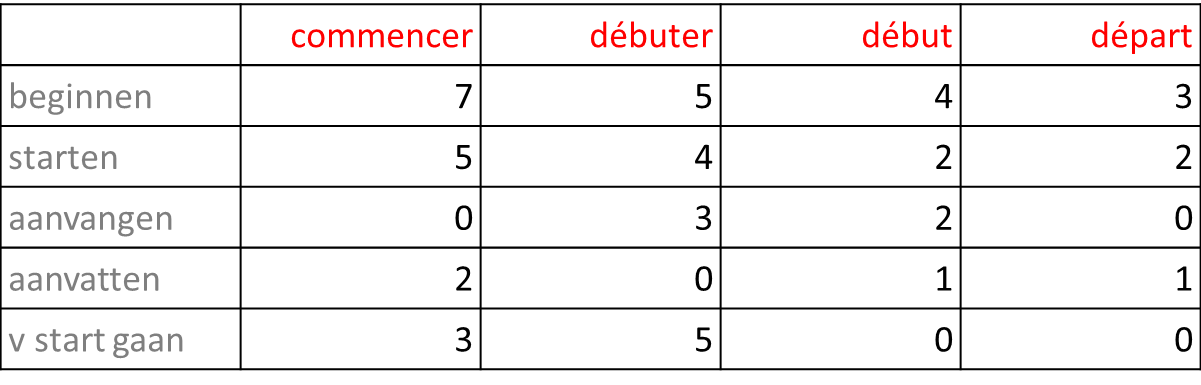
\includegraphics[height=.3\textheight]{figures/Vandevoorde2-img15.png}
\end{table}

The initial map has as many dimensions as there are columns in the data matrix (\figref{fig:3:16}).

\begin{figure}
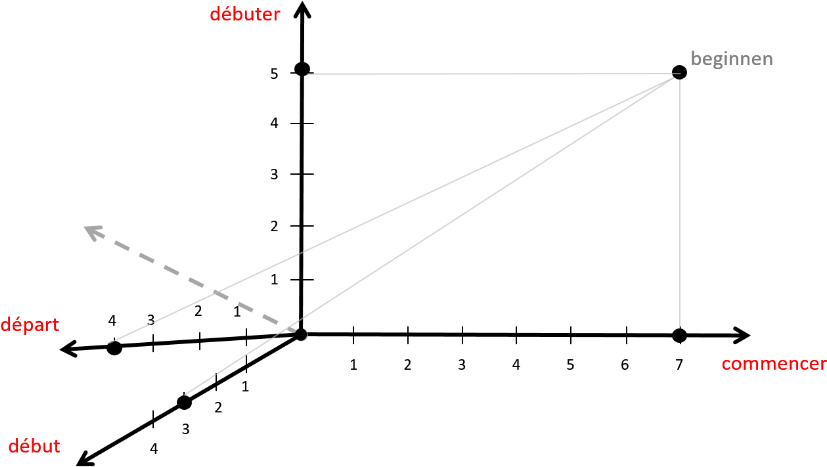
\includegraphics[height=.3\textheight]{figures/Vandevoorde2-img16.png}
\caption{Spatial map with $n$ dimensions for \textit{beginnen} \label{fig:3:16}}
\end{figure}

Now, in order to be able to visually present the specific geographic position of each of the Dutch lexemes in the rows, their position in the n-dimensional space is reduced to a two-dimensional space. All five Dutch lexemes can then be  represented as points in this space (\figref{fig:3:17}).

\begin{figure}
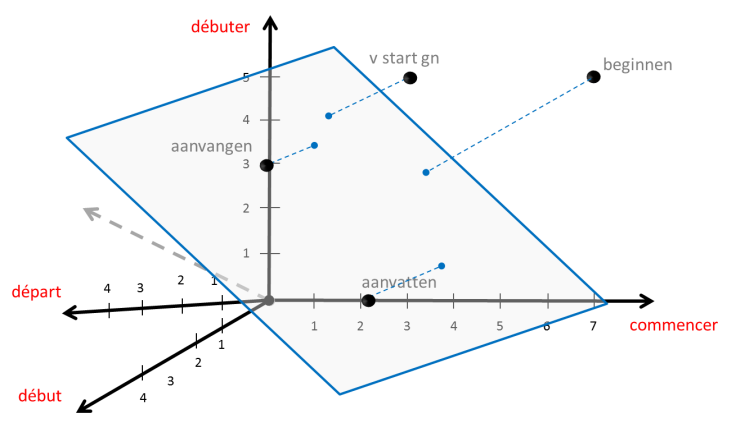
\includegraphics[height=.3\textheight]{figures/Vandevoorde2-img17.png}
\caption{Reduction to a two dimensional space for all rows \label{fig:3:17}}
\end{figure}

Next, the best fitting two-dimensional space is computed (\figref{fig:3:18}). Because this two-dimensional map captures the original high-dimensional data cloud as much as possible, it is true that “the larger the distance between two rows, the further these two rows should be apart in the map for rows” \citep[129]{baayen_analyzing_2008}. Consequently, the positions of the lexemes and the distances between the plotted lexemes represent the similarities and differences between the lexemes. The same computation is repeated for the columns of the frequency table and the simultaneous representation of the row map and the column map results in a so-called bi-plot (representing the scatterplot of the row map and the scatter plot of the column map simultaneously) (\figref{fig:3:18}). When CA is applied to the data sets gathered for this study, a first visualization via CA of the SourceDutch field of \textit{beginnen} is obtained (\figref{fig:3:19}).

\begin{figure}[p]
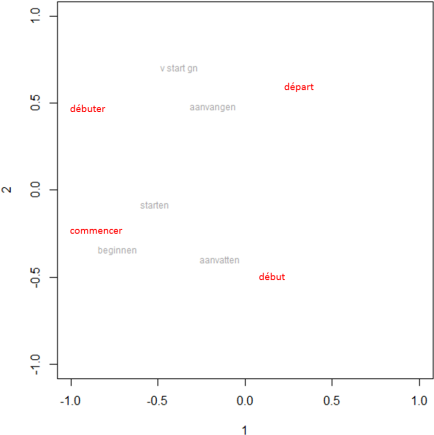
\includegraphics[width=7cm]{figures/Vandevoorde2-img18.png}
\caption{\label{fig:3:18}Bi-plot for fictitious data matrix in \tabref{tab:3:12}}
\end{figure}

\begin{figure}[p]
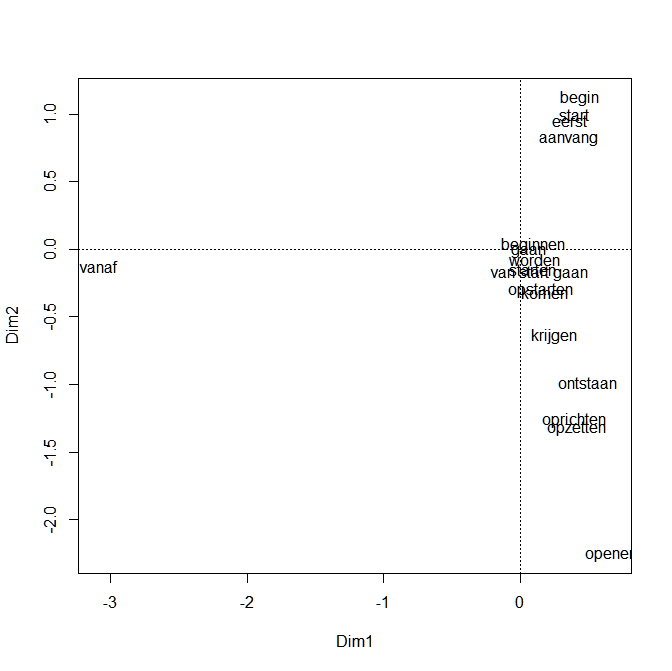
\includegraphics[width=7cm]{figures/Vandevoorde2-img19.png}
\caption{\label{fig:3:19}First Correspondence Analysis of SourceDutch field for \textit{beginnen}}
\end{figure}

What is immediately striking is the outlying position of \textit{vanaf}. Although the selection of lexemes has been done through a carefully developed technique, described in the previous sections, it is decided to exclude \textit{vanaf} from all data sets. Looking back at the frequency tables (the second T-images of \textit{beginnen}\textsubscript{ENG} and \textit{beginnen}\textsubscript{FR}, see Tables~\ref{appendix:E} and~\ref{appendix:F} in Appendix~\ref{ch:A}) for SourceDutch, it is indeed striking that \textit{vanaf} has, what can be called, an “unusual profile” \citep[92]{greenacre_correspondence_2007}: \textit{vanaf} is related to a single French target lexeme, i.e. \textit{à} \textit{partir} \textit{de}. In the second T-image of \textit{beginnen}\textsubscript{FR}, we also see that the relative weight of \textit{vanaf} is rather high (0.1505792; representing 15\% of the total number of observations) and contributing to a 0.1953608 – over 19\% – rise of the total inertia\footnote{“1. The (total) inertia of a table quantifies how much variation is present in the set of row profiles or in the set of column profiles […] 3. CA is performed with the objective of accounting for a maximum amount of inertia along the first axis. The second axis accounts for a maximum of the remaining inertia, and so on. […]” \citep[88]{greenacre_correspondence_2007}.} of the data matrix when compared to the same data matrix without \textit{vanaf}. The conclusion is that the variation of the first dimension is solely accounted for by \textit{vanaf}. \citet[92]{greenacre_correspondence_2007} indeed warns for the fact that outliers can “start to dominate a map so much that the more interesting contrasts between the more frequently occurring categories are completely masked”. The data points in the plot without \textit{vanaf} (\figref{fig:3:26}) are indeed more spread out in the two-dimensional space, which will facilitate the interpretation. Based on the above, \textit{vanaf} is removed from all data sets.

Before I further analyze a visualization via CA, the degree of representativeness of the plots with respect to the total variation in each of the data sets needs to be assessed. The measure for variation in a frequency table is the inertia \citep{greenacre_correspondence_2007}. The distribution of inertia over the latent dimensions of the CA can be visualized in a so-called scree plot: the bars show how much of the total variation is associated with each dimension. Consequently, the scree plot indicates how many dimensions are needed to reach a threshold, e.g. 80\%. The scree plots for SourceDutch, TransDutch\textsubscript{ENG} and TransDutch\textsubscript{FR}, show that five dimensions are required for SourceDutch (Figure~\ref{fig:3:20}), three dimensions for TransDutch\textsubscript{ENG} (Figure~\ref{fig:3:22}) and four dimensions for TransDutch\textsubscript{FR} (Figure~\ref{fig:3:24}) in order to represent 80\% of the total variation visually. This presents a practical problem, however, as 4- or 5-dimensional plots are not easily visualized. Although a visualization via CA for SourceDutch only represents around 40\% of the inertia, the visualization in \figref{fig:3:26} is presented as a first, exploratory analysis of the field of SourceDutch.

\begin{figure}
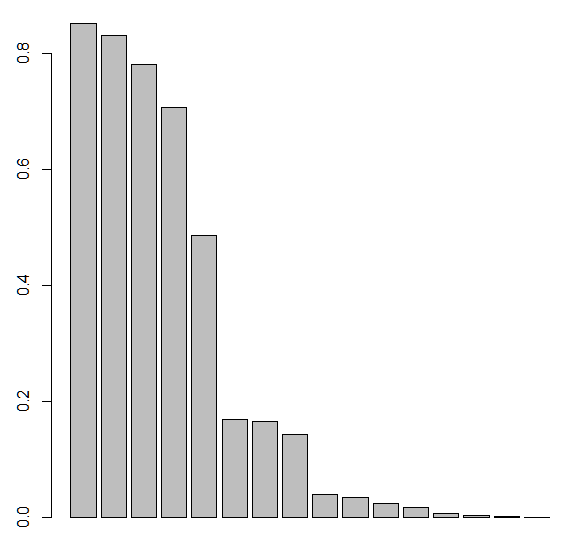
\includegraphics[width=.48\textwidth]{figures/Vandevoorde2-img20.png}\hfill%
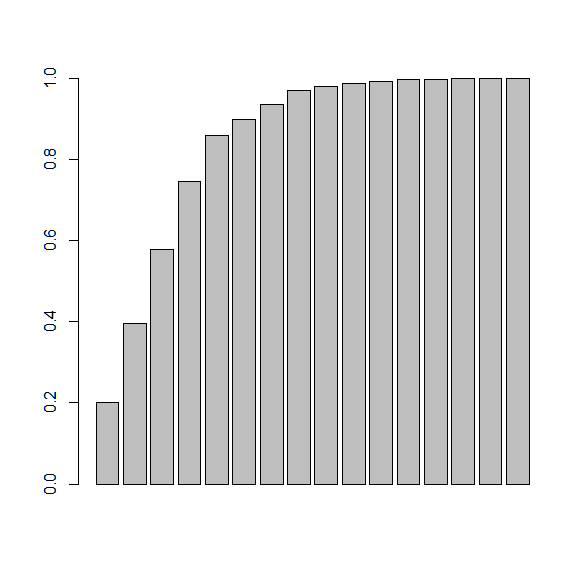
\includegraphics[width=.48\textwidth]{figures/Vandevoorde2-img21.png}
\caption{Left: \label{fig:3:20}Scree plot for SourceDutch. Right: \label{fig:3:21}Cumulative scree plot for SourceDutch.}
\end{figure}

\begin{figure}
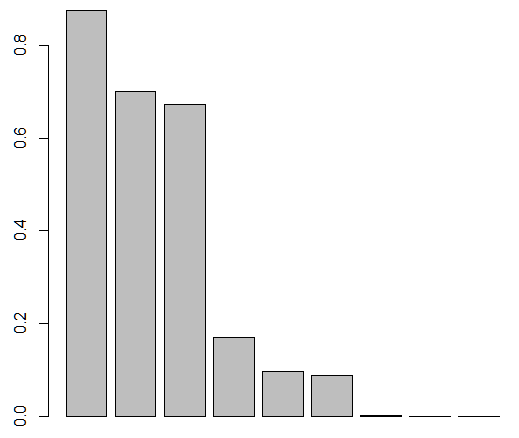
\includegraphics[width=.48\textwidth]{figures/Vandevoorde2-img22.png}\hfill%
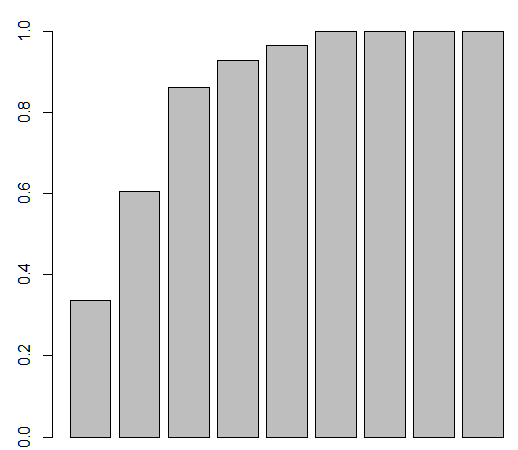
\includegraphics[width=.48\textwidth]{figures/Vandevoorde2-img23.png}
\caption{Left: \label{fig:3:22}Scree plot for TransDutch\textsubscript{ENG}. Right: \label{fig:3:23}Cumulative scree plot TransDutch\textsubscript{ENG}}
\end{figure}

\begin{figure}
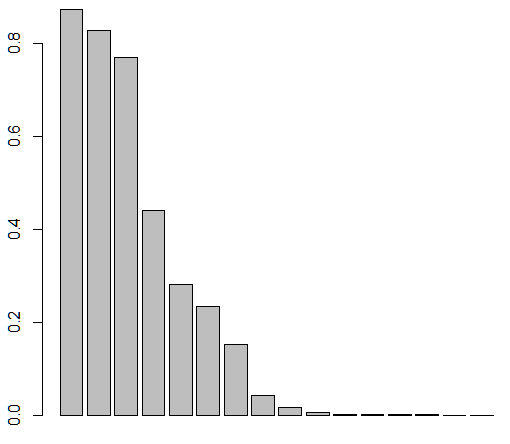
\includegraphics[width=.48\textwidth]{figures/Vandevoorde2-img24.png}\hfill%
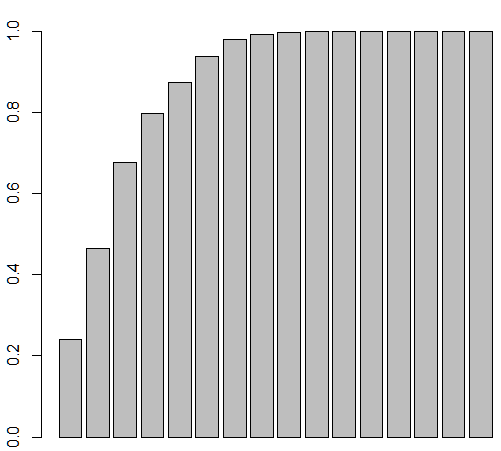
\includegraphics[width=.48\textwidth]{figures/Vandevoorde2-img25.png}
\caption{Left: \label{fig:3:24}Scree plot for TransDutch\textsubscript{FR}. Right: \label{fig:3:25}Cumulative scree plot for TransDutch\textsubscript{FR}.}
\end{figure}

\begin{figure}
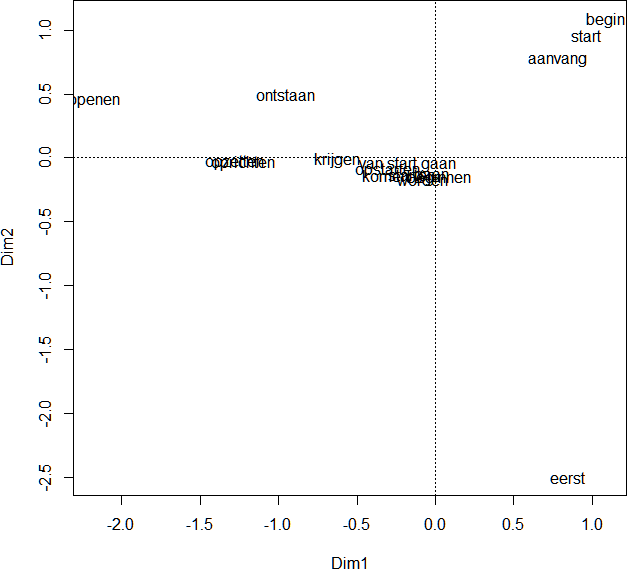
\includegraphics[width=7cm]{figures/Vandevoorde2-img26.png}
\caption{\label{fig:3:26}Correspondence Analysis of SourceDutch field for \textit{beginnen} without \textit{vanaf}}
\end{figure}

In \figref{fig:3:26}, one large central cluster is observed, situated around the origin (the ``zero-point'') of the plot which contains, amongst other lexemes, the initial lexeme \textit{beginnen}. This central cluster is considered as the prototypical center, consisting of lexemes with the basic meaning of the inchoative category, viz. “start of a general process”. In the upper right corner, a second cluster contains \textit{aanvang} `commencement', \textit{start} `start' and \textit{begin} `beginning'; all three lexemes are nouns, where \textit{start} and \textit{begin} are the nominal derivatives of \textit{beginnen} and \textit{starten} (which belong to the cluster considered as the prototypical center). The third lexeme \textit{aanvang} then, is the more formal\footnote{In order to underpin the assertions presented with respect to the pragmatics or semantics of a given lexeme, I rely on information retrieved in the lexical database Cornetto \citep{spyns_cornetto:_2013}.} counterpart of \textit{begin} and \textit{start}. In the lower right corner, \textit{eerst} `firstly' holds a somewhat outlying position. This outlying position can be explained by the fact that the translations which determine its position (\textit{d’abord} and \textit{firstly}) are almost exclusively used as translations of \textit{eerst}. \textit{Oprichten} `to establish' and \textit{opzetten} `to set up' are furthermore clustering together. In the lexical database Cornetto \citep{vossen_cornetto_2008, spyns_cornetto:_2013}, \textit{oprichten} is defined as \textit{opzetten} and both verbs are indicated to refer to inchoative situations involving a project, a business, a company, etc. In other words, the CA confirms the strong relation between the two lexemes. Finally, \textit{ontstaan} `to come into being' and \textit{openen} `to open' occupy a somewhat unclear position between the center and periphery of the graph. On the basis of the CA, three different clusters can be discerned: one central cluster (considered as the one with the most prototypical expressions of inchoativity); one cluster containing the nominal derivatives of \textit{beginnen} and \textit{starten} plus \textit{aanvang}, a small third cluster with the near-synonymous verbs \textit{oprichten} and \textit{opzetten}. It is not entirely clear whether \textit{ontstaan} and \textit{openen} could be considered as one cluster, or whether they should be considered as two separate, singleton clusters.

Due to the subtlety of the semantic field, the delimitation of clearly distinct clusters can appear difficult. A drawback of CA moreover is that it does not allow to further analyze the central cluster: the visualization only suggests that the lexemes within this cluster are closely related, but the exact relations remain unclear.

Conclusively, the following observations can be made on the basis of this preliminary CA. Firstly, an outlying data point which was distorting the overall interpretation of the data (\textit{vanaf}) was detected and removed. Secondly, the scree plots for SourceDutch, TransDutch\textsubscript{ENG} and TransDutch\textsubscript{FR} showed that for these data sets, more than 2 dimensions are required to accurately represent the distribution of the inertia over the latent dimensions of the CA. This represents a practical problem with respect to visualization. Thirdly, a first exploration of the SourceDutch field on the basis of the CA allowed to formulate some preliminary insights into the semantic field. However, the delimitation of clearly distinct clusters appeared difficult and the exact relations between the lexemes in the central cluster could not further be examined. It was therefore decided to use Hierarchical cluster Analysis for the visualization of the semantic fields of SourceDutch, TransDutch\textsubscript{ENG} and TransDutch\textsubscript{FR}. The HCA will be carried out on the output of a CA, a procedure which will be further explained in the next section.

\subsection{Hierarchical Cluster Analysis}
\label{sec:3.7.2}  
Hierarchical Cluster Analysis (HCA) can be defined as “a collection of different algorithms that puts objects into clusters according to well-defined similarity rules” and is “mostly used when we do not have any a priori hypotheses” \citep[406]{glynn_cluster_2014}. In this section, I will first describe which type of cluster analysis seems the best choice for this study. In addition, as every cluster analysis is crucially dependent on both a particular similarity measure and clustering algorithm, I will elaborate on these measures in \sectref{sec:3.7.2.1} and \sectref{sec:3.7.2.2} respectively. Next, I will explain the procedure for determining the number of clusters for which I will rely on the R package \texttt{pvclust} \citep{suzuki_pvclust:_2006} (\sectref{sec:3.7.2.3}). Finally, I propose a validation of the combined choice of a particular similarity measure and clustering algorithm and of the number of clusters in the cluster solution (\sectref{sec:3.7.2.4}).\footnote{Exhaustive overviews of the existing clustering techniques can be found in \citet[495--523]{manning_foundations_1999}, \citet[138--148]{baayen_analyzing_2008},  \citet[71--110]{everitt_cluster_2011}, \citet[336--349]{gries_statistics_2013} and \citet{glynn_cluster_2014}.}

Just as semantic spaces are customary in computational semantics, in (cognitive) linguistics, “[c]luster analyses have been used to determine the similarity of intraword senses or the degree of granularity exhibited by polysemous word senses (cf. \citealt{steinberg_empirical_1971,sandra_network_1995,putz_prepositional_1996})” (\citealt[81]{gries_corpus-based_2006}). The method has also been extensively used by Gries and Divjak (see for example \citealt{divjak_structuring_2010,glynn_cluster_2014,divjak_ways_2006, evans_behavioral_2009,gries_corpus-based_2006,evans_behavioral_2009,gries_behavioral_2010,deshors_case_2014}). The reasons for HCA’s popularity are summarized by Divjak:

\begin{quote}
Cluster analysis is one of the basic exploratory techniques that are often applied in analyzing large data sets. This statistical method helps organize observed data into meaningful structures: it finds similarities between elements and groups similar elements together. These groupings, in turn, assist in understanding relationships that might exist among these elements. In other words: cluster analysis finds the most optimal solution and organizes an enormous number of data in substructures that facilitate comparison of the (elements in the) structures to each other \citep[129--130]{divjak_structuring_2010}.
\end{quote}

HCA is not a single technique, but covers “a family of techniques for clustering data and displaying them in a tree-like format” \citep[138]{baayen_analyzing_2008}. In Statistical NLP, HCA has two main uses: exploratory data analysis on the one hand and generalization on the other hand \citep[497]{manning_foundations_1999}. The tree-like format in which the result of a clustering algorithm can be visually represented is called a dendrogram:

\begin{quote}
a branching diagram where the apparent similarity between nodes at the bottom is shown by the height of the connection which joins them. Each node in the tree represents a cluster that was created by merging two child nodes. [...] The “height” of the node corresponds to the decreasing similarity of the two clusters that are being merged \citep[495]{manning_foundations_1999}.
\end{quote}

In order to maintain terminological clarity, I propose to use the following terminology (visualized in \figref{fig:3:27}), which is to a large extent based on \citet[89]{everitt_cluster_2011}. A \textit{node} can refer to either an \textit{internal} \textit{node}, a \textit{sub-node} (an internal node within one delimited cluster) or a \textit{terminal} \textit{node} (also called a \textit{leaf}). The \textit{heights} of the \textit{edges} can be read off from the dendrogram. The line perpendicular to the edges in the tree is called the \textit{root}. Finally, I will call the names printed at the extremities of every terminal node \textit{lexemes} or \textit{lexical} \textit{items} (which is an immediate adaptation of the terminology to the type of data in this book) instead of the term \textit{label} proposed by \citet{everitt_cluster_2011}. 

\begin{figure}
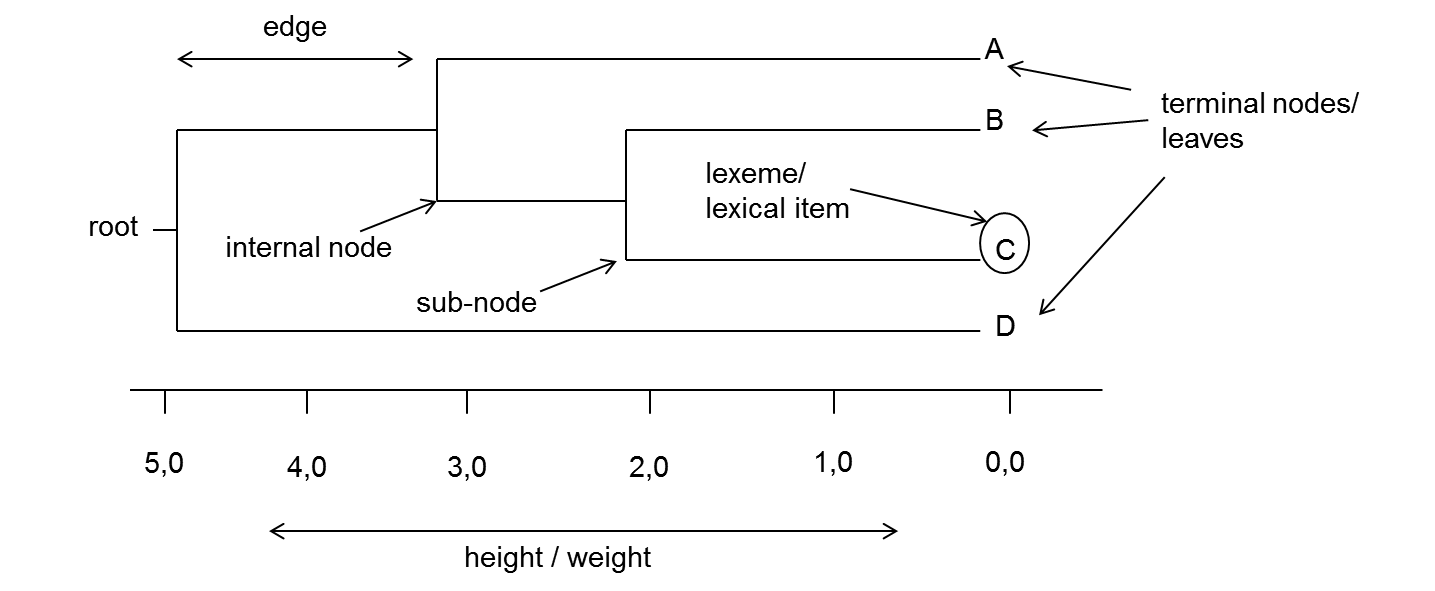
\includegraphics[width=\textwidth]{figures/Vandevoorde2-img27.png}
\caption{\label{fig:3:27}Terminological description of a dendrogram (adapted from \citealt[89]{everitt_cluster_2011})}
\todo[inline]{The use of ``n,m'' separated by a comma might not be the best option. Please consider writing ``n/m'' if n refers to height and m to weight or ``n.m'' if it is an one-dimensional value}
\end{figure}

HCA comes in two flavors: the \textit{tree} can be constructed either top-down or bottom-up. The first method is called divisive clustering where “one starts with all the objects and divides them into groups so as to maximize within-group similarity” \citep[501]{manning_foundations_1999}. The second method is called agglomerative clustering which works “by starting with the individual objects and grouping the most similar ones \citep[500--501]{manning_foundations_1999}”. Divisive clustering – also called partitioning – is known to have difficulties in finding “optimal divisions for smaller clusters” and appears to be better at finding a few large clusters \citep[138]{baayen_analyzing_2008}. This can be verified by the visualized result in \figref{fig:3:28}, which shows a so-called \textsc{chaining effect} when applying divisive clustering for TransDutch\textsubscript{ENG}. This means that the cluster tree displays “a chain of large similarities without taking into account the global context” \citep[504]{manning_foundations_1999}. As Manning and Schütze argue, cluster analysis is normally based on “the assumption that ``tight'' clusters are better than ``straggly'' clusters”, and that this in turn “reflects an intuition that a cluster is a group of objects centered around a central point, and so compact clusters are to be preferred” \citep[506]{manning_foundations_1999}. In particular, this corresponds to “a model like the Gaussian distribution” \citep[506]{manning_foundations_1999}. Although Manning and Schütze stress that this is “only one possible underlying model of what a good cluster is”, and that a good clustering should rely on prior knowledge or a model of the data, “elongated clusters” due to a chaining effect are usually disfavored to sphere-shaped clusters \citep[506]{manning_foundations_1999}. Because the dendrograms will be interpreted as semantic fields of \textit{beginnen}, organized in a prototype-based manner – with the different clusters representing the meaning differentiations of the lexeme under study – I will prefer a clustering which indeed reflects my intuition that the clusters are centered around a central point and avoids large, elongated clusters caused by a chaining effect.

In summary, I follow \citet[92]{everitt_cluster_2011} who state that the chaining effect is a symptom of distortion through “space contraction” where “dissimilar objects are drawn into the same cluster” \citep[92]{everitt_cluster_2011}. Everitt and colleagues point out that a second type of distortion exists, called \textsc{space-dilation} which takes place “where the process of fusing clusters tends to draw clusters together” \citet[92]{everitt_cluster_2011}. \figref{fig:3:29} illustrates such a space-dilation effect, of which I will also be wary.

\begin{figure}%%[Warning: Draw object ignored]
% 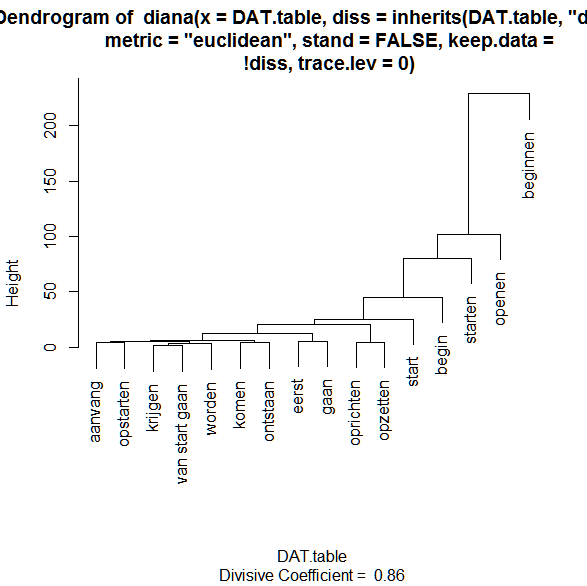
\includegraphics[height=.3\textheight]{figures/Vandevoorde2-img28.png}
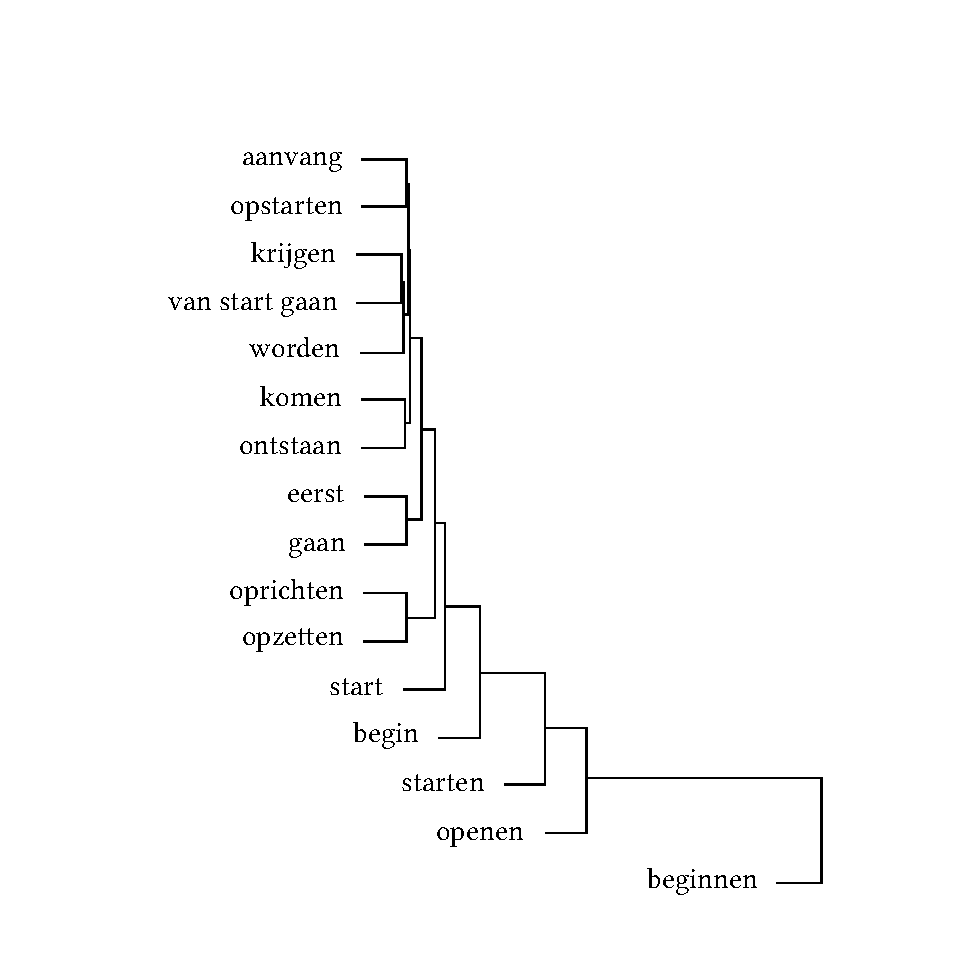
\includegraphics[height=.4\textheight]{figures/tree28.pdf}
Chaining effect
\caption{\label{fig:3:28}Divise clustering of the field of TransDutch\textsubscript{ENG}, displaying chaining effect\todo[inline]{Chaining effect not displaying correctly. I need information where exactly the arrow should point and the description be placed.}}
\end{figure}

\begin{figure}%%[Warning: Draw object ignored]
% 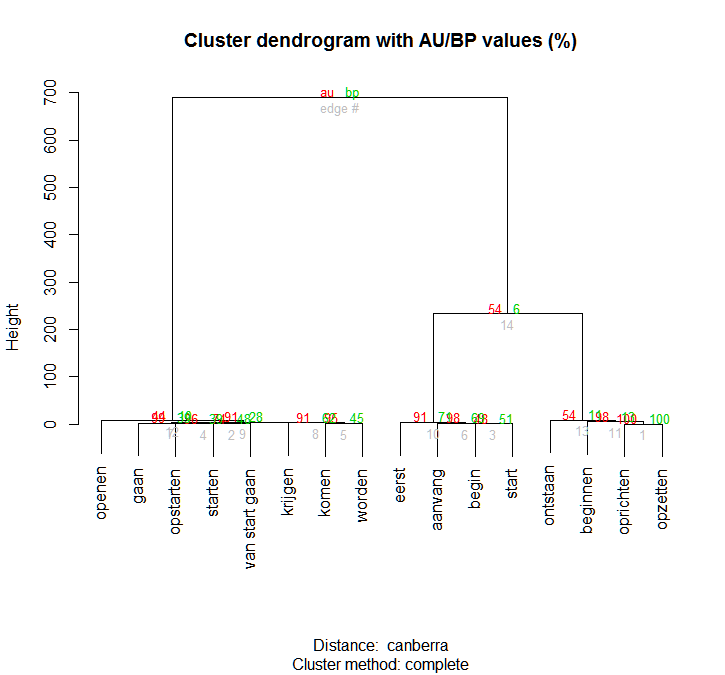
\includegraphics[height=.3\textheight]{figures/Vandevoorde2-img29.png}
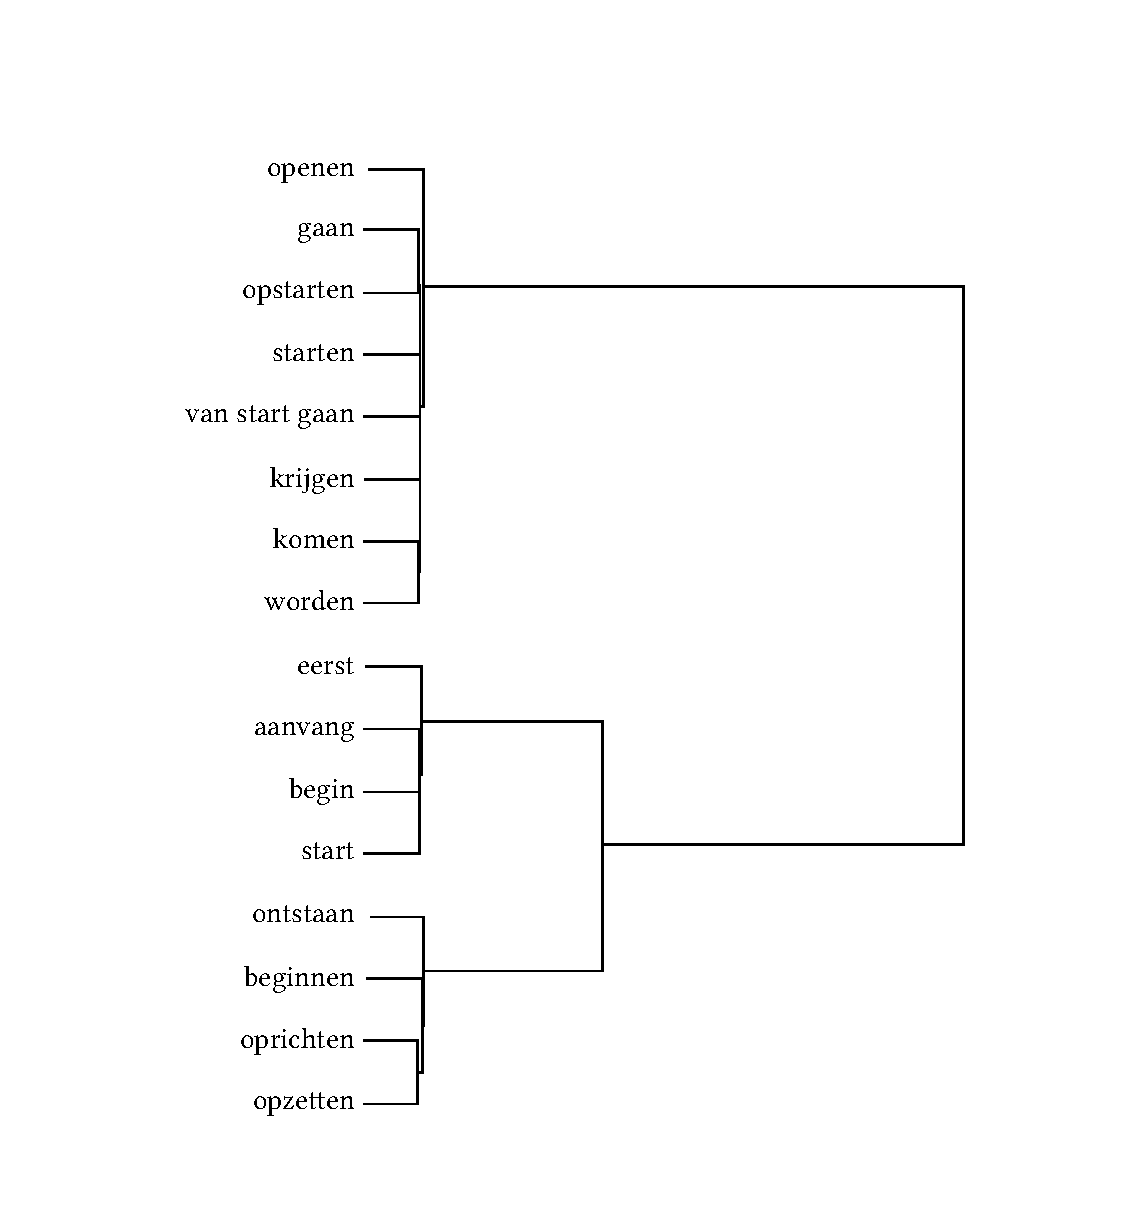
\includegraphics[height=.4\textheight]{figures/tree29.pdf}
Space dilation
\caption{\label{fig:3:29} Agglomerative clustering of the field of SourceDutch, displaying space-dilation\todo[inline]{Space dilation not displaying correctly. I need information where exactly the arrow should point and the description be placed.}}
\end{figure}

As a consequence, the data will be further explored with hierarchical agglomerative clustering (HAC). In addition, the HAC will be carried out on the resultant coordinates of the CA. I thereby follow \citet[335]{cuadras_correspondence_1993} who suggest “to complement it [a CA] with a classification”, as this “can supply elements of information that could have been hidden by the projection onto a low dimensional subspace” (see also \citealt[28]{ciampi_correspondence_2005}). A HAC performed on the output of a CA has obvious advantages as CA involves dimension reduction: noisy dimensions are omitted and only informative dimensions are retained. By selecting only the informative dimensions of the CA as input for the HAC, such an analysis is likely to be better interpretable than a HAC on raw data. In other words, this procedure ``combines the best of two worlds'': CA allows to detect informative dimensions of variation to the detriment of noise, and with HAC meaningful structure(s) in the data cloud can be discerned.

Since I will use the output of the CA as input for a HAC, I use the \texttt{fast\_sca()} function of the \texttt{svs}-package to obtain the coordinates (the coordinates can also be obtained by applying the \texttt{ca()} function in R). The \texttt{svs}-function \texttt{fast\_sca()} is especially designed to further use the resultant coordinates of a CA as the input for an additional analysis.

\subsubsection{(Dis)similarity measure}
\label{sec:3.7.2.1}
Clustering algorithms depend crucially on similarity which is understood as “its everyday meaning of how similar entities are” \citep[411]{glynn_cluster_2014}. For numerical variables, similarities are often converted into dissimilarities (or distance). This can be done by subtracting the measure of similarity from 1. In this way, 0 indicates minimum dissimilarity and 1 maximum dissimilarity \citep[415--416]{glynn_cluster_2014}. There is a wide variety of distance measures, but I will limit the comparison to two measures which are customarily used in linguistics: the Euclidean distance and the Canberra distance, the latter is known to handle sparse data and zero-occurrences best \citep[132]{divjak_structuring_2010}. Based on the outcome of the comparison (which will be presented in \sectref{sec:3.7.2.4}), Euclidean will be chosen as the distance measure for the analyses in this book.

\subsubsection{Clustering algorithm}\label{sec:3.7.2.2}  
Next to an appropriate distance measure, a clustering algorithm also depends on a so-called amalgamation rule. This determines “which clusters are merged in each step in bottom-up clustering” \citep[503]{manning_foundations_1999}. In fact, the amalgamation rule is the defining feature of the various agglomerative cluster algorithms as it specifies in which way the proximity between two clusters will be computed; “the definition of cluster proximity that differentiates the various agglomerative hierarchical techniques” \citep[517]{tan_introduction_2006}. The most important cluster algorithms are the following:

\begin{description}
\item[Single-link clustering] (also called nearest neighbor or single-linkage algorithm) considers the similarity between two clusters as “the similarity of the two closest objects in the clusters” \citep[503]{manning_foundations_1999}. This algorithm is known to produce locally coherent clusters, but with a bad global quality \citep[503]{manning_foundations_1999}; the clusters moreover tend to show a chaining effect \citep[504]{manning_foundations_1999}.

\item[Complete-link clustering] (also called furthest neighbor or complete-linkage algorithm) “focuses on global cluster quality [...]. The similarity of two clusters is the similarity of their two most dissimilar members” \citep[505]{manning_foundations_1999}. This algorithm is known to avoid chaining effect, which is preferable in NLP applications \citep[506]{manning_foundations_1999}.

\item[Group-average agglomerative clustering] (or average-linkage) is a compromise between the previous two algorithms, which uses the average similarity as a criterion to merge items into clusters \citep[507]{manning_foundations_1999}. It can be considered as an alternative to complete-link clustering and it is also known to avoid chaining effect.

\item[Ward’s Minimum Variance Method] is a somewhat different clustering algorithm as it “allows two clusters to merge if the increase in sum of squared distances\footnote{The sum of squares is a measure of variation, calculated by summing the squares of the differences from the mean.} of the members of the new cluster from their mean is smaller than for any other possible merger between two clusters. Use of squared distances penalizes spread out clusters and so results in compact clusters without being as restrictive as complete-linkage” \citep[426]{glynn_cluster_2014}. Because of its tendency to find spherical clusters, Ward’s Method is “a frequently recommended strategy that yields small clusters” \citep[133]{divjak_structuring_2010}.
\end{description}

The above mentioned algorithms can themselves be grouped according to the different views on clusters they reflect. Depending on the goals one defines, different types of clusters can be found useful. \citet[493--495]{tan_introduction_2006} distinguish five types of cluster solutions: well-separated clusters (each object in a cluster is closer or more similar to every other object in the cluster than to any object not in the cluster), prototype-based clusters (each object in the cluster is closer or more similar to the prototype that defines the cluster than to the prototype of any other cluster), graph-based clusters (nodes are seen as objects; the links represent connections among the objects), density-based clusters (a cluster is seen as a dense region of objects surrounded by a region of low density) and shared-property clusters (also called conceptual clusters, where a cluster is a set of objects that share some property). Single-linkage, complete-linkage and average-linkage algorithms suit a graph-based view of clusters; Ward’s Method, on the other hand, is the more natural choice when one adheres a prototype-based view on clusters, since it “assumes that a cluster is represented by its centroid [...]” \citep[517]{tan_introduction_2006}.

Which cluster algorithm is the ``right'' one for this purpose, is not a trivial question, as different algorithms yield different dendrograms. \citet[132]{divjak_structuring_2010}, following \citet[35]{speece_cluster_1994} emphasizes choosing the algorithms whose “``side-effects'' of the mathematical properties [...] fit the phenomenon under investigation, and, consequently, yield easily interpretable results”. 

The single-linkage method is discarded because of its tendency to produce a chaining effect. For the other cluster algorithms, however, it is not so clear which method is preferable. From the previous descriptions, Ward’s Method seems to suit my needs best: it can yield small clusters – as a “side-effect of its mathematical properties” – and it reflects a prototype-based view on clusters. The choice of Ward’s Minimum Variance method is also what results from the comparison with the complete and average-linkage methods in \sectref{sec:3.7.2.4}. HAC is carried out on the output of the CA with the function \texttt{pvclust()} from the package \texttt{pvclust} which relies on the function \texttt{hclust()} (the choice of \texttt{pvclust} will be substantiated in the next section).

\subsubsection{Number of clusters}\label{sec:3.7.2.3}\largerpage
An important issue of HAC concerns the choice of the number of clusters, i.e. the ``optimal cluster solution''. This is obtained by ``cutting'' the tree at a particular height into $n$ clusters. The height of the tree cut must be chosen carefully, as the resulting clusters will be considered as meaningful and informative in the subsequent interpretation. There is, however, no straightforward procedure to determine the ``best cut''. As a rule of thumb, several scholars suggest that looking at the length of the vertical lines in the dendrogram is indicative for the ``optimal cluster solution''. Gries mentions that “large vertical lines indicate more autonomous subclusters” (\citeyear[338]{gries_statistics_2013}). Similarly, \citet[430]{glynn_cluster_2014} propose to “look at the height bar and choose a place where the cluster structure remains stable for a long distance”. Finally, \citet[95]{everitt_cluster_2011} assert that “large changes in fusion levels are taken to indicate the best cut”. Divjak \& Fieller admit that such suggestions are not exactly what we would call “frivolous” (\citeyear[430]{glynn_cluster_2014}). To somewhat remedy this, they mention three criteria which can help to make a decision on the cut height. According to \citet[432--433]{glynn_cluster_2014}, a ``good'' cut height should give (i) enough clusters in the solution for it to be meaningful (i.e. an acceptable size); (ii) an immediately intuited meaning for each\slash most of the clusters and (iii) criterion validity (the expected level of association between rows and columns should be acceptably reflected). \citet[432--433]{glynn_cluster_2014} furthermore propose two ways to investigate the robustness of a cluster solution: the computation of the average silhouette width and the use of bootstrap validation.

The optimal cluster solution will be determined by means of a bootstrap validation technique (I will use average silhouette width as a cluster validation technique, as explained further on in this section). Bootstrapping entails that the data are resampled (with replacement) a high number of times (usually 3000) in order to see how many times the same points are clustered together again. On the basis of these replications a $p$-value is computed for each node of the dendogram (i.e. the place where two branches join). As a consequence, the bootstrap $p$-values represent a measure of quality for each node. This bootstrap validation will be done with the R package \texttt{pvclust} \citep{suzuki_pvclust:_2006}. As a matter of fact, the \texttt{pvclust} package provides both an “approximately unbiased $p$-value” and a “bootstrap probability” (the use of the former is recommended by Suzuki \& Shimodaira). In addition, the package has the function \texttt{pvrect()} which can be used to cut the dendrogram at the nodes above a certain confidence level, e.g. 95\%. This has a clear advantage over tree cuts at a fixed height. Fixed-height cuts are common in HAC but not indispensable. \citeauthor{everitt_cluster_2011} warn that fixed-height cut methods require pre-established cut heights and minimum cluster size which can possibly be influenced by a priori expectations (\citeyear[95]{everitt_cluster_2011}).

If possible, I will always cut the tree at the highest significant node attaining a confidence level of 95\%. However, this procedure runs the risk of excluding many-cluster-solutions: e.g. if the two highest nodes in a tree are significant, \texttt{pvrect()} would choose a two-cluster-solution. Such solutions with very few clusters might be less interpretable than  many-cluster-solutions. As a consequence, I propose a compromise of cutting a dendrogram at a confidence level and cutting it at a fixed height: the cutoff point will be chosen so that for each cluster in the solution, the highest node within each cluster is significant (the Approximately Unbiased $p$-value should be $\geq 0.95$; an exception is made for singleton clusters). In this way the validated cluster solution meets the first two criteria mentioned by \citeauthor{glynn_cluster_2014} for good cut height (acceptable cluster size and meaningful clusters).

\subsubsection{Validation of the number of clusters}\label{sec:3.7.2.4}
In \sectref{sec:3.7.2.3} bootstrap $p$-values were proposed to determine the number of clusters. That procedure is now complemented with two techniques for testing the validity of a cluster solution. The first validation consists in the computation of the average silhouette widths proposed by \citet{kaufman_finding_1990}, the second one is a (non-hierarchical) $k$-means clustering.

\citet{kaufman_finding_1990} propose to calculate the silhouette width for each object in a cluster solution and summarize this information in a silhouette plot. For each object $i$, one can “compare $i$’s separation from its cluster against the heterogeneity of the cluster” \citep[138]{everitt_cluster_2011}. The silhouette width has a value situated between \textminus1 and 1. Values close to 1 imply that “the heterogeneity of object $i$’s cluster is much smaller than its separation and object $i$ is taken as ``well classified''” \citep[128]{everitt_cluster_2011}; values close to \textminus1 imply misclassification and values around 0 suggest that the classification is unclear \citep[128]{everitt_cluster_2011}. Finally, the average silhouette width – the average of all silhouette widths of a set of data – can be used to validate the chosen cluster solution. \citet{kaufman_finding_1990} point out that an average silhouette width above 0.5 indicates a good classification, whereas values beneath 0.2 betray an unclear classification. In addition, \citet[129]{everitt_cluster_2011} suggest using the average silhouette widths as an instrument for optimizing the number of clusters. The average silhouette width can be calculated using the \texttt{pam()} function of the cluster{}-package.

Although $k$-means clustering can be run as a separate clustering procedure, I will use it as a validation of the HAC. More specifically, I will compute the centers of the clusters from the HAC and feed those into a $k$-means clustering. If the partitioning of the lexemes into clusters remains (largely) the same in the $k$-means clustering, then this can be considered as a validation of the results in the HAC. After calculation of the cluster centroids using \texttt{centers\_ca()} function of \texttt{svs}, $k$-means clustering can be carried out using the \texttt{kmeans()} function. In contrast to HAC, which does not need a pre-determined number of clusters, non-hierarchical clustering methods such as $k$-means clustering require a pre-specified number of clusters. More specifically, $k$-means “defines the clusters by the center of mass of their members” \citep[515]{manning_foundations_1999}, i.e. it takes $k$ points as the centers of the clusters. For the initialization of the $k$-means algorithm, K points can be randomly chosen from the data to serve as seeds, although predetermined centers can also be supplied \citep[515]{manning_foundations_1999}. The algorithm then consists in iteratively assigning each data point to the cluster to the center of which it is closest \citep[515]{manning_foundations_1999} and subsequently recomputing the centers on the basis of the assignments \citep[515--516]{manning_foundations_1999}. This iterative procedure is carried out until convergence, i.e. until there are no further reassignments.

In \sectref{sec:3.7.2}, I substantiated my choice to carry out a HAC on the output of a CA. In addition to this procedure, it is also possible to carry out a HAC directly on the raw data or to compute the distances for the HAC on the output of a Latent Semantic Analysis. LSA is typically considered as a Vector Space Model since “the values of the elements are derived from event frequencies” \citep[144]{turney_frequency_2010} and it is also generally associated with distributional approaches to meaning \citep[141]{turney_frequency_2010}. Conceptually, LSA works as follows:

\begin{quote}
LSA projects document frequency vectors into a low dimensional space calculated using the frequencies of word occurrence in each document. The relative distances between these points are interpreted as distances between the topics of the documents \citep[123]{mehler_models_2007}.
\end{quote}

LSA can, by virtue of its symmetry, also be applied to word similarity \citep[123]{mehler_models_2007} and consequently also to translational similarity. In this case, the algorithm of LSA (which is usually applied to a document-term matrix) is applied to a source–target language matrix.

In the subsequent comparison, I will include HAC on the raw data and HAC on the output of a LSA. The various combinations of distance measures (Euclidean and Canberra), amalgamation rules (Complete, Average and Ward’s) and spatial maps (raw data, output of CA, output of LSA) are summarized in \tabref{tab:3:13}. Because of the high number of combinatorial possibilities – 18 in total – I only compare the combinations for the data set SourceDutch. I selected three validation criteria which have in common their ability to assess the overall strength of the clustering structure: agglomerative coefficient, chaining effect and $p$-values.

Firstly, the agglomerative coefficient for each combination is calculated. This is a standard measure to describe the strength of a clustering structure.

\begin{quote}
The agglomerative coefficient (AC) [is] a measure of the clustering structure of the data set that can range from 0 to 1. An AC close to 1 indicates that a very clear structuring has been found whereas an AC close to 0 indicates that the algorithm has not found a natural structure. This measure is sensitive to sample size, i.e. the value grows with the number of observations \citep[426]{glynn_cluster_2014}.
\end{quote}

Since I am using the same data set for each dendrogram in this comparison, the agglomerative coefficients are comparable. An agglomerative coefficient higher than 0.80 is considered as satisfactory.

Secondly, the output for each combination is visually inspected for presence of chaining effect. For this study, a chaining effect in the cluster structure is disfavored to a sphere-like structure. Hence, the appearance of a chaining effect (as well as of a space-dilation effect) will be considered negative. Because a chaining effect can only be determined on the basis of visual inspection, we introduced four levels of chaining. In \tabref{tab:3:13}, \textit{no} means that no chaining effect was observed, \textit{yes} that a clear chaining effect was observed, \textit{high} means that chaining occurs only in the higher nodes and \textit{low} means that chaining only occurs in the lower nodes. Only those results where a clear chaining effect is observed (\textit{yes}), will be considered negative, no chaining (\textit{no}) will be considered as the most positive outcome.

Finally, the $p$-values (which were introduced in \sectref{sec:3.7.2.3} to determine the cluster solution) will be used as a third element to assess the overall strength of the clustering structure. To do so, the number of significant nodes (i.e. with a $p$-value of 0.95 or higher) in the dendrogram will be counted. Each of the dendrograms presented in the comparison counts 14 nodes. If $\geq 7$ nodes in the dendrogram are significant, this will be considered as an indication of a strong overall clustering structure. The number in the third column of \tabref{tab:3:13} thus indicates the number of significant $p$-values ($\geq 0.95$) on a total of 14 nodes.

\begin{table}\caption{Combinatory possibilities of the selected distance measures, clustering algorithms and ``spatial maps''. \textsuperscript{†}: (+ high space dilation)\label{tab:3:13}}
\begin{tabular}{llrlr} 
\lsptoprule
&  Procedural combination &  Agglomerative & {Chaining}  & {$p$-values}\\
&                         &  coefficient   & {effect} \\\midrule
1 & Euclidean, Average          & 0.72 & YES & 10\\
2 & Euclidean, Average, on CA   & 0.74 & YES & 10\\
3 & Euclidean, Average, on LSA  & 0.61 & YES & 8\\
4 & Euclidean, Complete         & 0.73 & YES & 10\\
5 & Euclidean, Complete, on CA  & 0.76 & YES & 9\\
6 & Euclidean, Complete, on LSA & 0.65 & high & 4\\
7 & Euclidean, Ward’s           & 0.78 & YES & 9\\
8 & Euclidean, Ward’s, on CA    & 0.89 & NO & 9\\
9 & Euclidean, Ward’s, on LSA   & 0.72 & NO & 4\\
10 & Canberra, Average          & 0.22 & high & 2\\
11 & Canberra, Average, on CA   & 0.95 & low\textsuperscript{†}  & 6\\
12 & Canberra, Average, on LSA  & 0.82 & NO & 6\\
13 & Canberra, Complete         & 0.27 & NO & 1\\
14 & Canberra, Complete, on CA  & 0.99 & low\textsuperscript{†} & 7\\
15 & Canberra, Complete, on LSA & 0.99 & low\textsuperscript{†} & 9\\
16 & Canberra, Ward’s           & 0.43 & NO & 2\\
17 & Canberra, Ward’s, on CA    & 0.99 & low\textsuperscript{†} & 5\\
18 & Canberra, Ward’s, on LSA   & 0.96 & NO & 3\\
\lspbottomrule
\end{tabular}
\end{table}

\tabref{tab:3:13} (and the accompanying Figures~\ref{fig:3:30}--\ref{fig:3:47}\footnote{For each figure, the number between brackets refers to the number of the combination in \tabref{tab:3:11} it represents. I will use these numbers to refer to the different combinations (not the Figure numbers).}) shows that combinations 8, 11, 12, 14, 15, 17 and 18 have an agglomerative coefficient higher than 0.80. It is noteworthy that only one combination with Euclidean distance reaches a satisfactory agglomerative coefficient. In addition, for the combinations with Canberra distance, none of the analyses carried out on the raw data display a satisfactory agglomerative coefficient.

Six out of nine combinations with Euclidean distance show a clear chaining effect (combinations 1, 2, 3, 4, 5 and 7). Combination 6 displays chaining on the higher edges of the dendrogram. Only combinations 8 and 9 (using Ward’s Minimum Variance Method) do not suffer from chaining. As for the combinations with Canberra distance, none of them displays clear chaining, although combinations 11, 14, 15 and 17 show space-dilation effects on the higher edges as well as chaining-effects on the lower edges. Combination 10 only shows some chaining on the higher edges. Combinations 12, 13, 16 and 18 show no effect of chaining nor space-dilation at all. Chaining and space-dilation effects seem not to be limited to the complete-linkage algorithm but appear irrespective of the clustering algorithm.

For the combinations with Euclidean distance, all but two combinations display a high number of significant $p$-values (only combinations 6 and 9, carried out on the output of a LSA have less than 7 significant nodes). For the combinations with Canberra distance, only two out of nine combinations have 7 or more significant $p$-values: combinations 14 and 15, both carried out with the complete-linkage algorithm.

On the basis of the obtained values for each of the criteria in the comparison, it can be concluded that combinations 8 (Euclidean, Wards, on CA), 14 (Canberra, Complete, on CA) and 15 (Canberra, Complete, on LSA) are most likely to yield interpretable results for these data. Preference goes to combination 8, because no chaining was observed at all (in combinations 14 and 15 space-dilation in the high nodes and chaining in the low nodes was observed). In addition, this is the only combination with Ward’s Method, which is a more natural choice when one adheres a prototype-based view on clusters (as was explained in \sectref{sec:3.7.2.2}). On the basis of this comparison, it is decided to apply combination 8 (Euclidean, Wards, on CA) to all data sets of the case study of \textit{beginnen.}

The previous comparison also leads to some more general observations: when Euclidean distance is used, chaining effect, relatively high agglomerative coefficients (although lower than for Canberra) and a high number of significant $p$-values are more likely to appear. Combining Euclidean distance with Ward’s Method seems to avoid chaining effects. Canberra distance, on the other hand, avoids chaining effect, renders high agglomerative coefficients (except on raw data) but renders a low number of significant $p$-values. From the point of view of the clustering algorithms, it is noteworthy that combinations with the complete-linkage algorithm usually display a high amount of significant $p$-values and that combinations with Ward’s Method are usually best at avoiding chaining effect (only combination 7 with Ward’s displays clear chaining). When the different spatial maps are taken as point of departure, it appears that analyses on the raw data render low agglomerative coefficients and that analyses on the CA are prone to chaining.

\begin{figure}
% 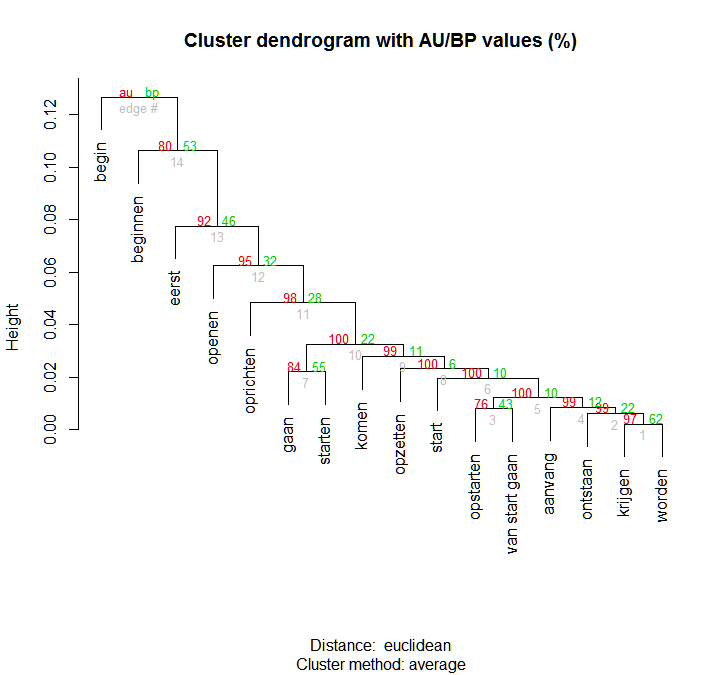
\includegraphics[height=.3\textheight]{figures/Vandevoorde2-img30.png}
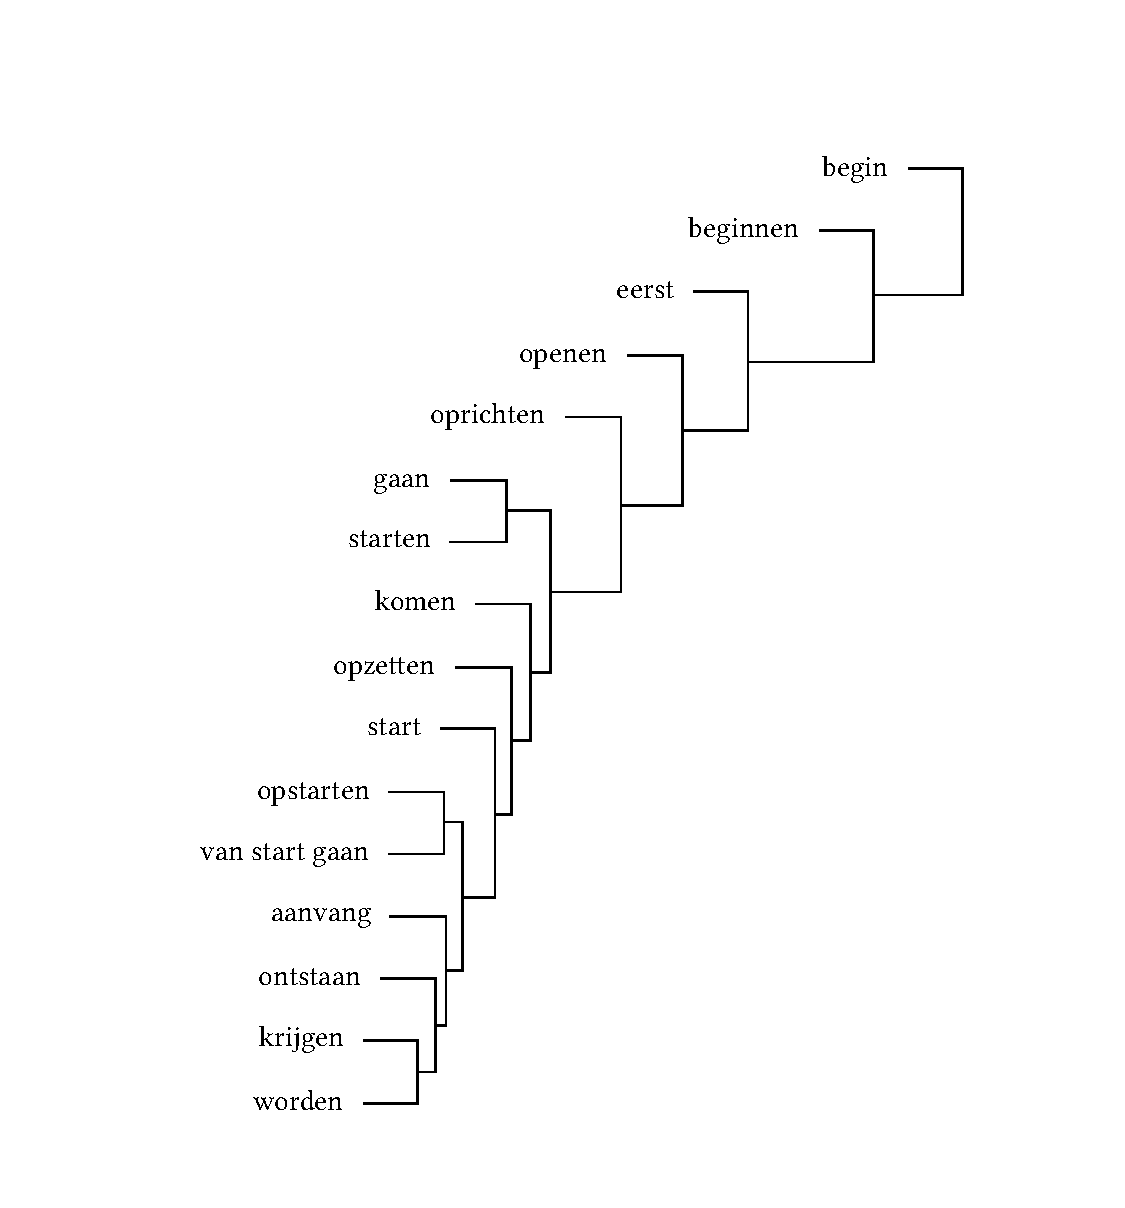
\includegraphics[width=.48\textwidth,trim=95 40 75 75]{figures/tree30.pdf}\hfill%
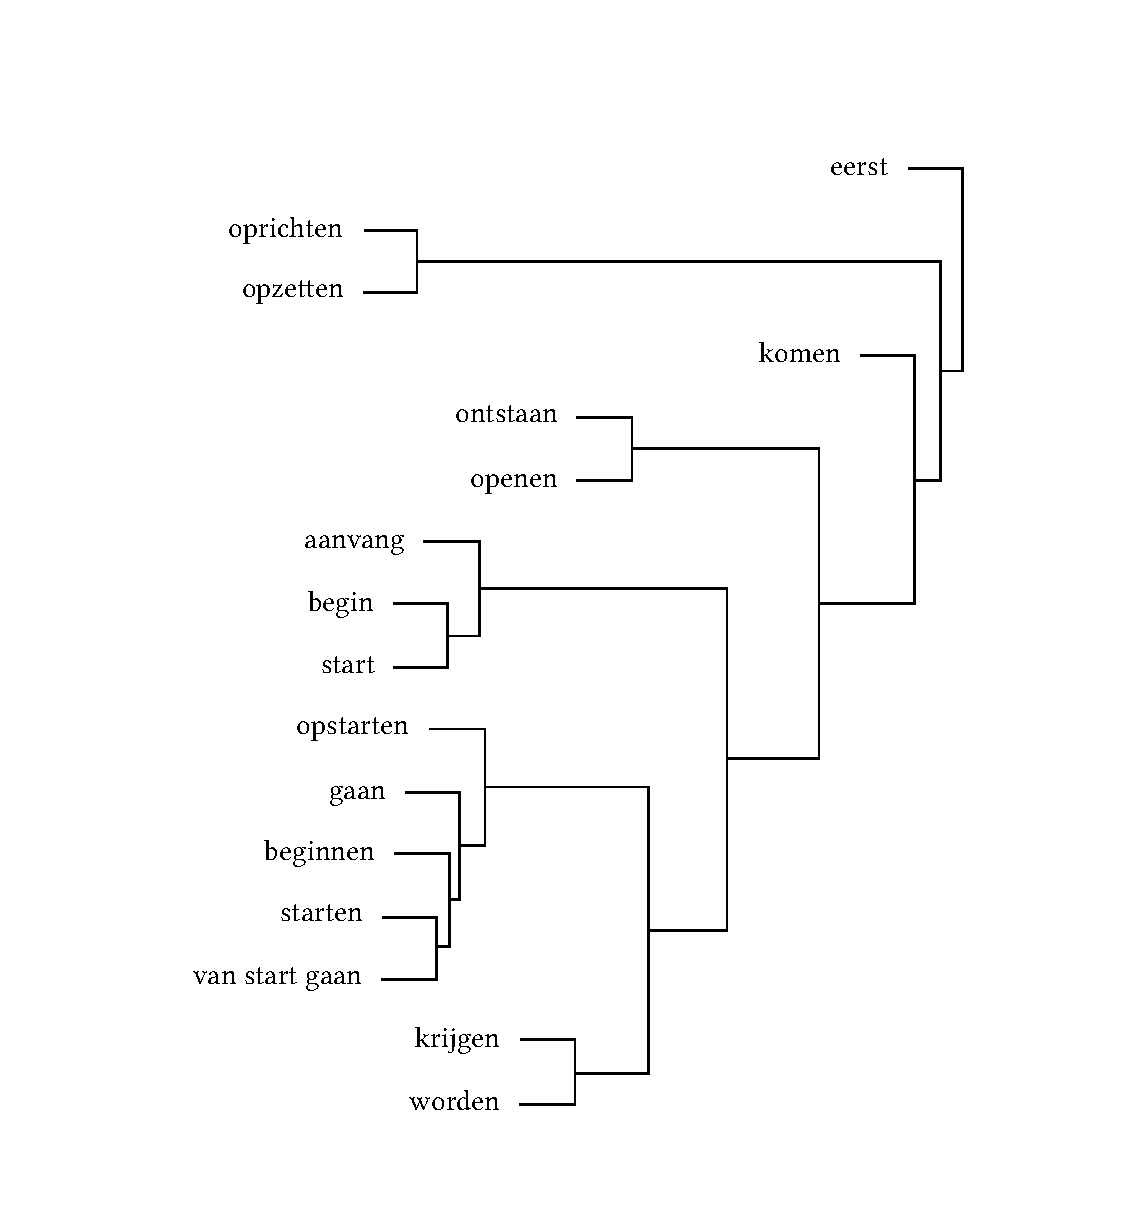
\includegraphics[width=.48\textwidth,trim=95 40 75 75]{figures/tree31.pdf}
\caption{\label{fig:3:30}Left: Euclidean, Average (1). Right:\label{fig:3:31} Euclidean, Average, on CA (2).}
\end{figure}

\begin{figure}
% 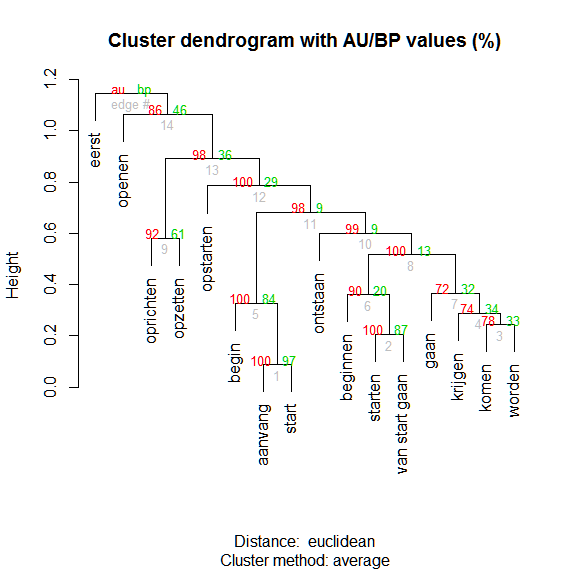
\includegraphics[height=.4\textheight]{figures/Vandevoorde2-img32.png}
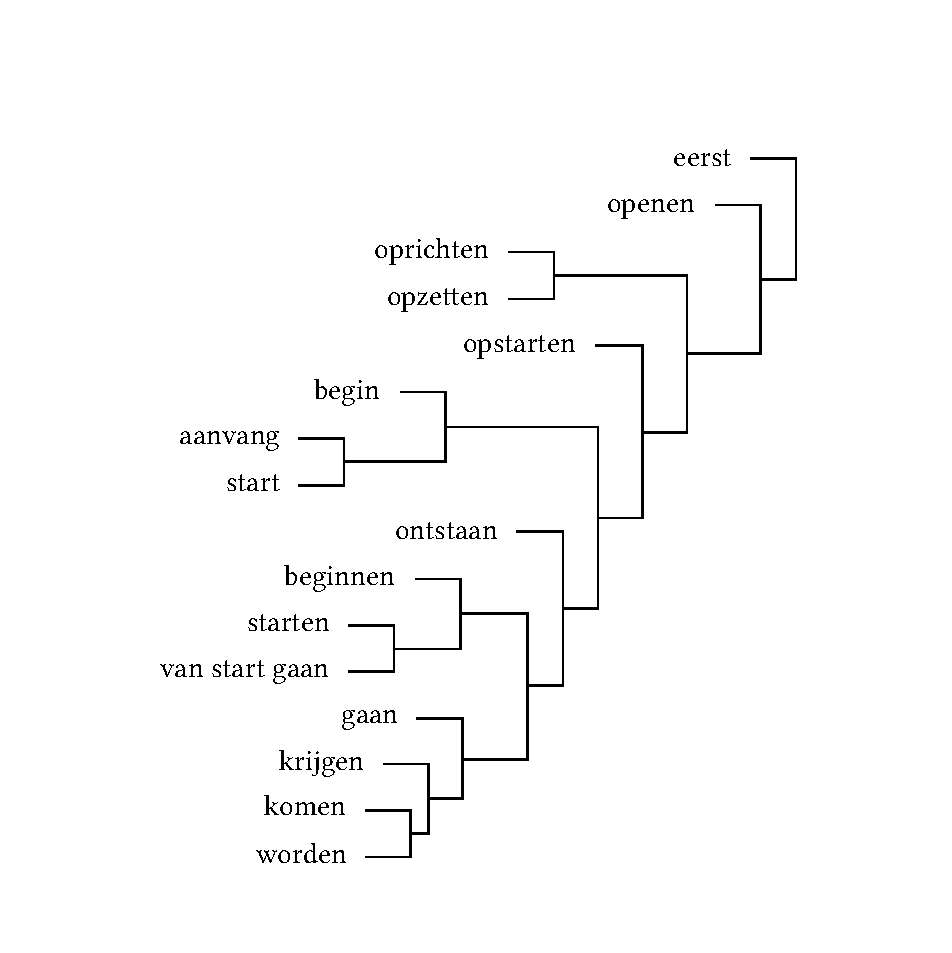
\includegraphics[width=.48\textwidth,trim=95 40 75 75]{figures/tree32.pdf}\hfill%
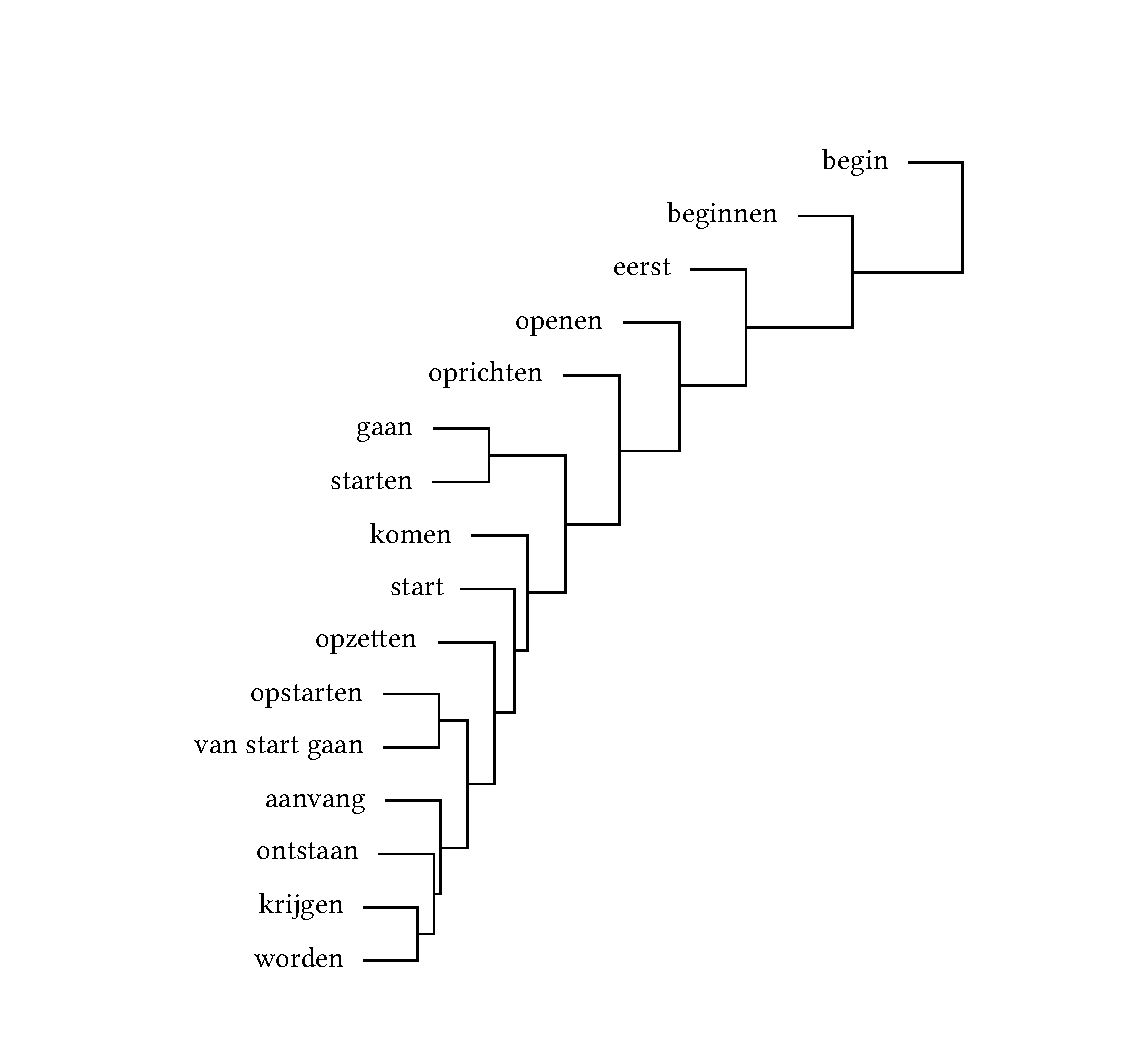
\includegraphics[width=.48\textwidth,trim=95 40 75 75]{figures/tree33.pdf}
\caption{Left:\label{fig:3:32} Euclidean, Average, on LSA (3). Right:\label{fig:3:33}  Euclidean, Complete (4).}
\end{figure}

\begin{figure}
% 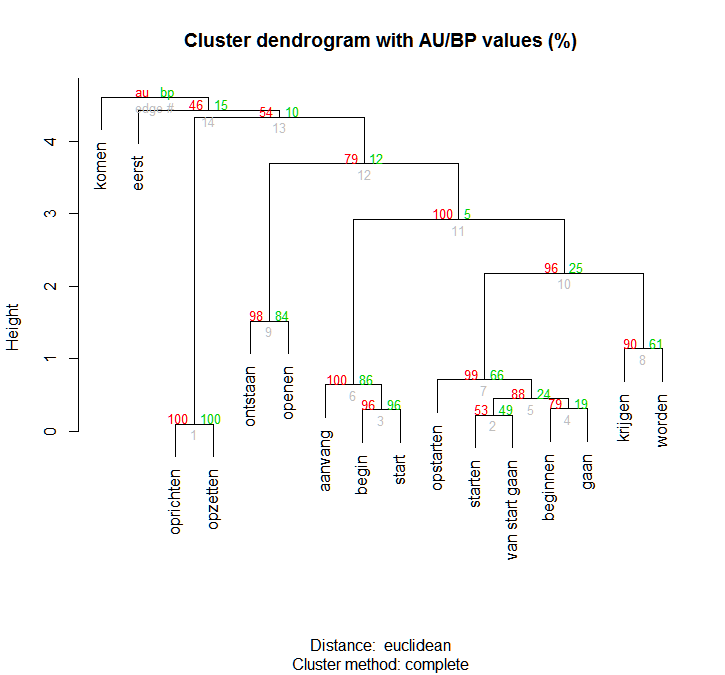
\includegraphics[height=.4\textheight]{figures/Vandevoorde2-img34.png}
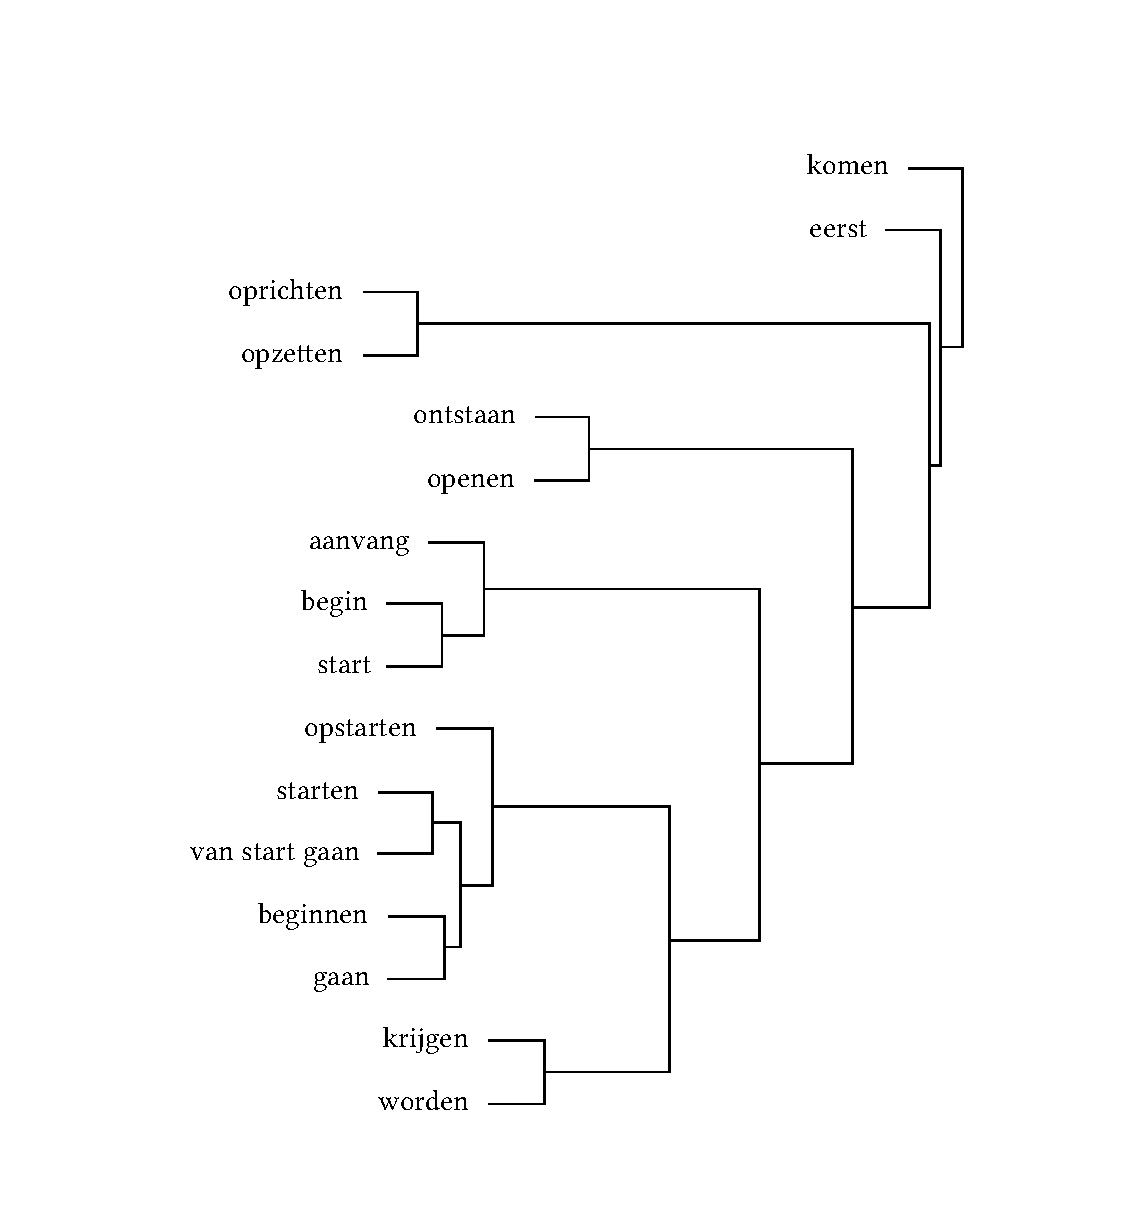
\includegraphics[width=.48\textwidth,trim=95 40 75 75]{figures/tree34.pdf}\hfill%
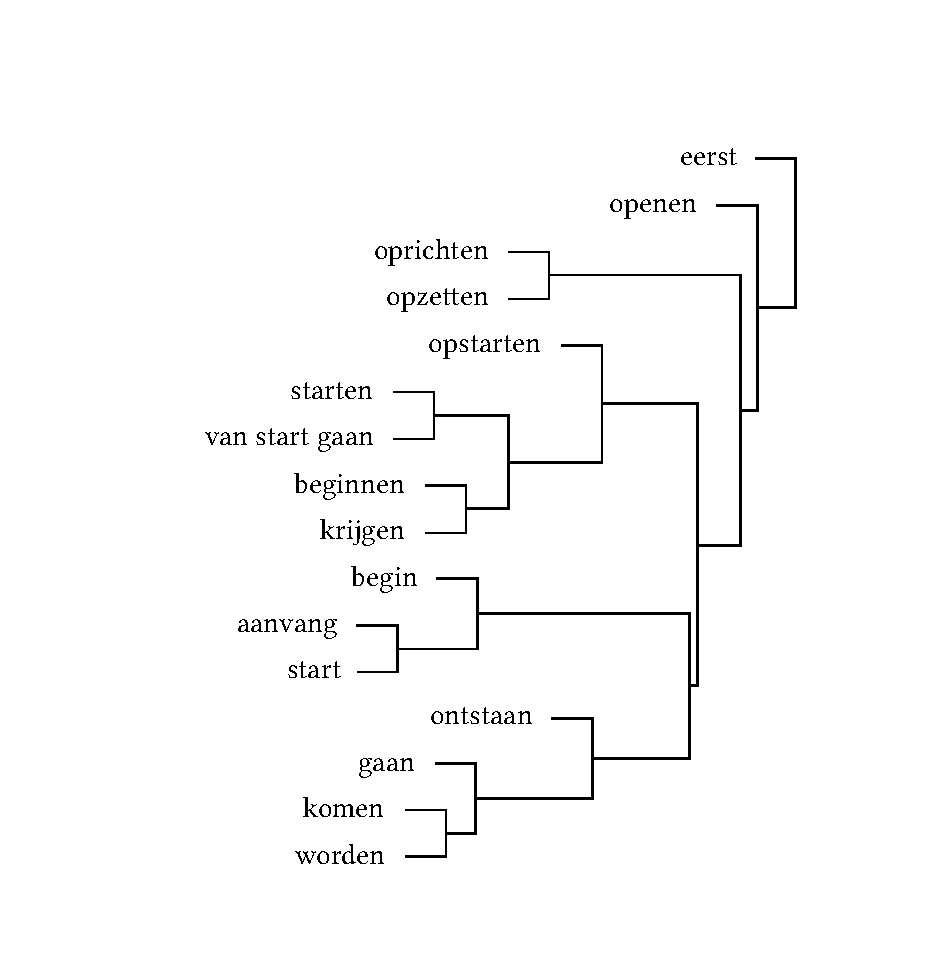
\includegraphics[width=.48\textwidth,trim=95 40 75 75]{figures/tree35.pdf}
\caption{\label{fig:3:34}Left: Euclidean, Complete, on CA (5).\label{fig:3:35}Right: Euclidean, Complete, on LSA (6).}
\end{figure}

\begin{figure}
% 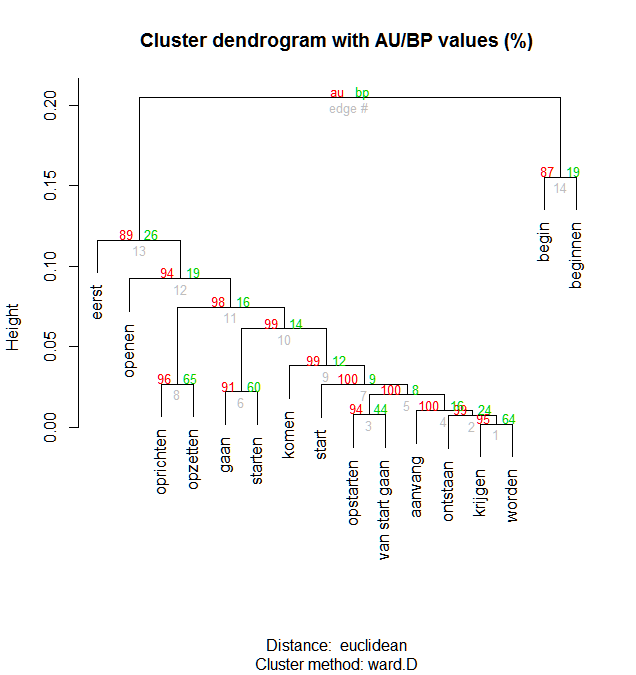
\includegraphics[width=.48\textwidth,trim=95 40 75 75]{figures/Vandevoorde2-img36.png}
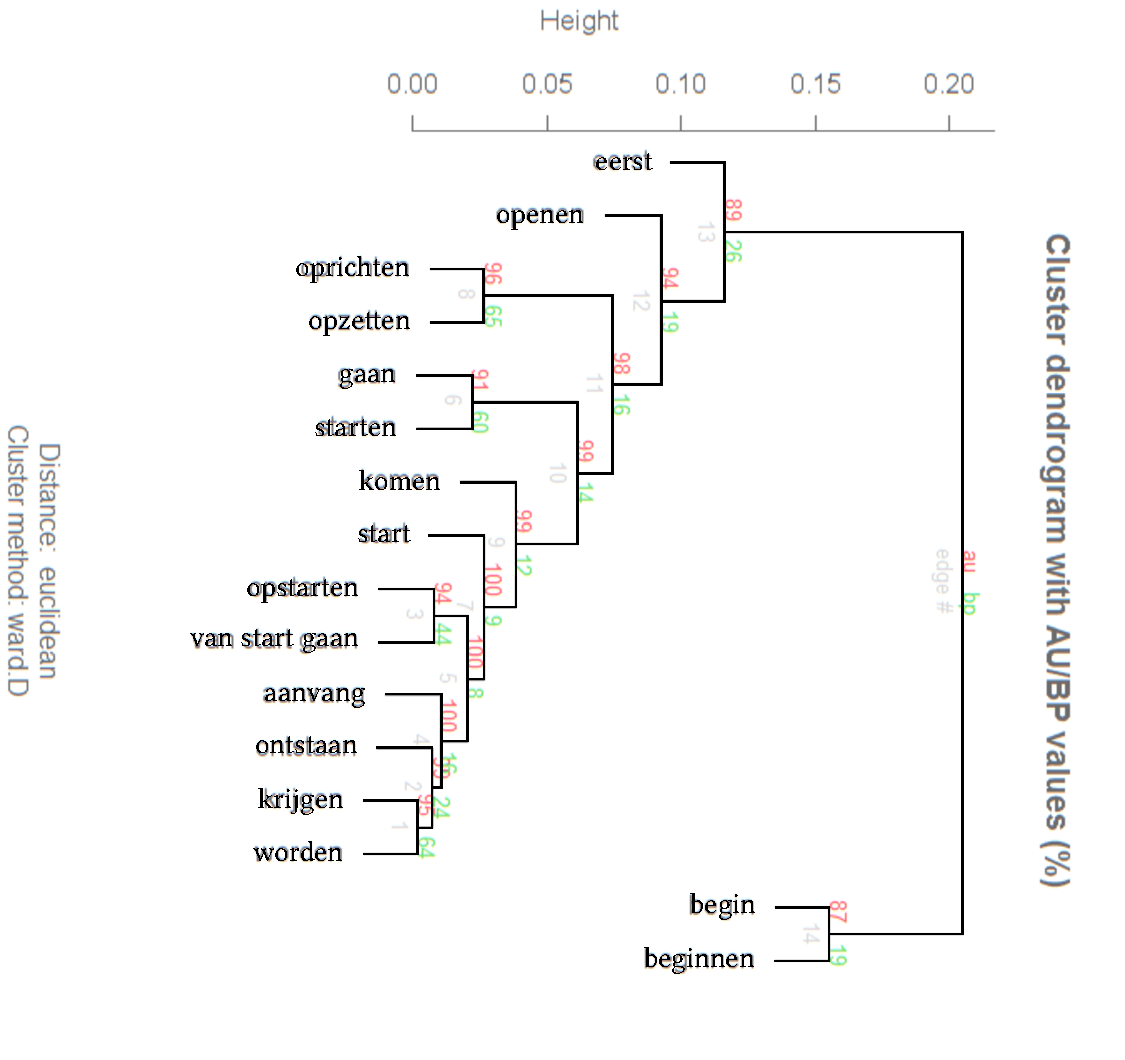
\includegraphics[width=.48\textwidth,trim=95 40 75 75]{figures/tree36.pdf}\hfill%
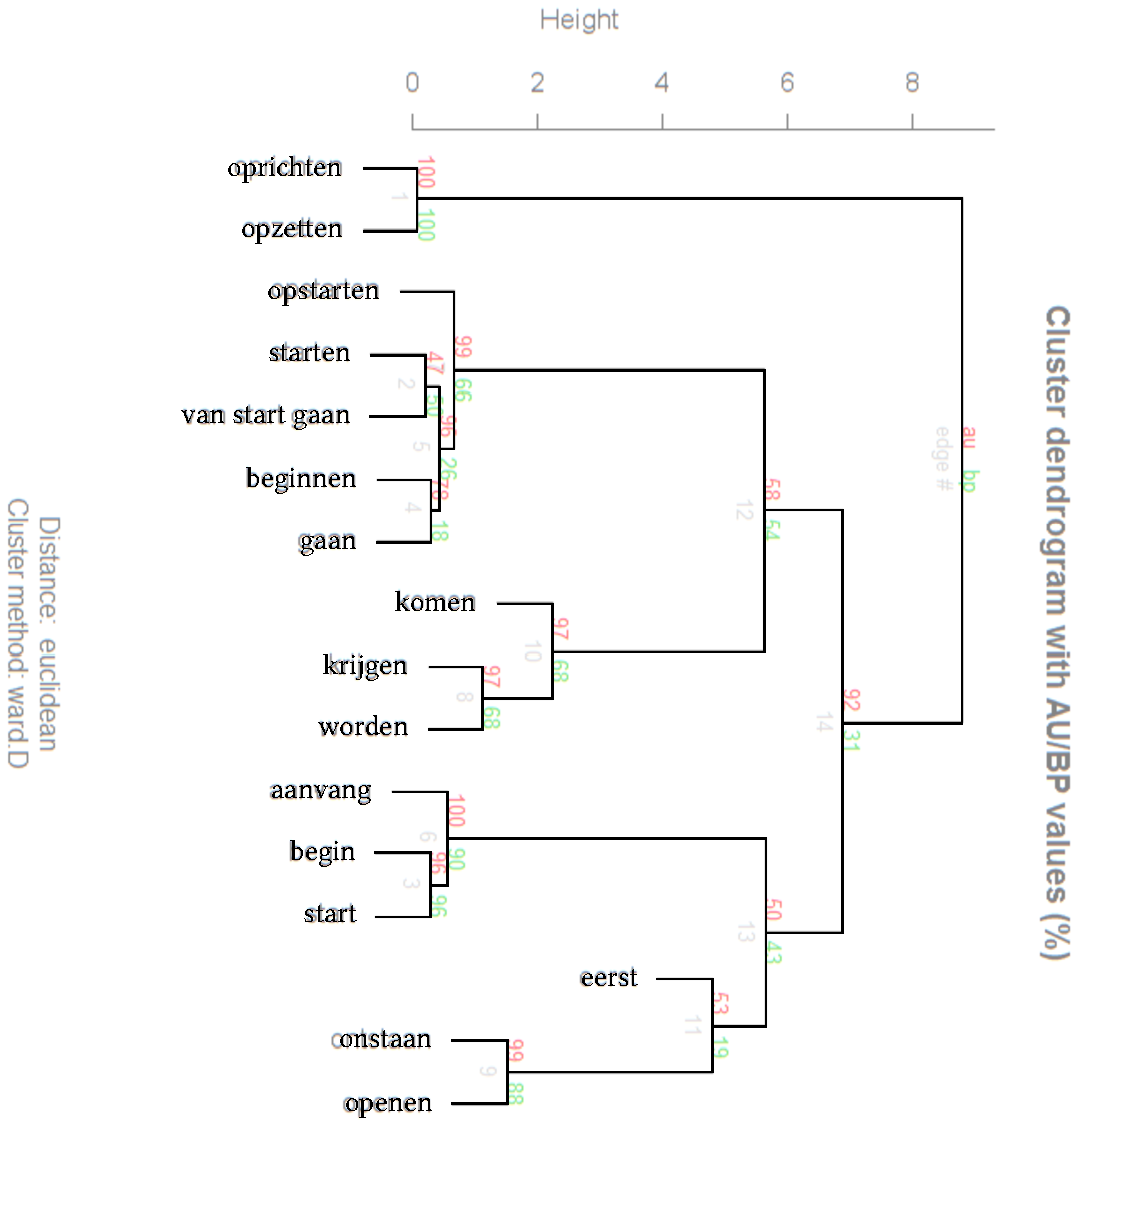
\includegraphics[width=.48\textwidth,trim=95 40 75 75]{figures/tree37.pdf}
\caption{\label{fig:3:36}Left: Euclidean, Ward’s (7). Right:\label{fig:3:37} Euclidean, Ward’s, on CA (8).}
\end{figure}

\begin{figure}
% 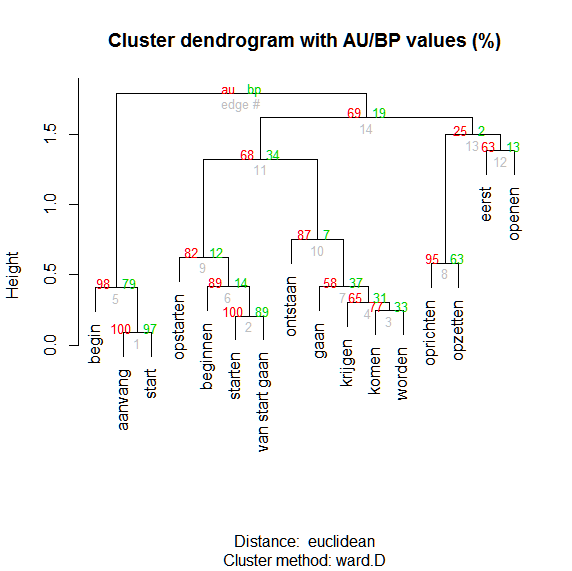
\includegraphics[width=.48\textwidth,trim=95 40 75 75]{figures/Vandevoorde2-img38.png}
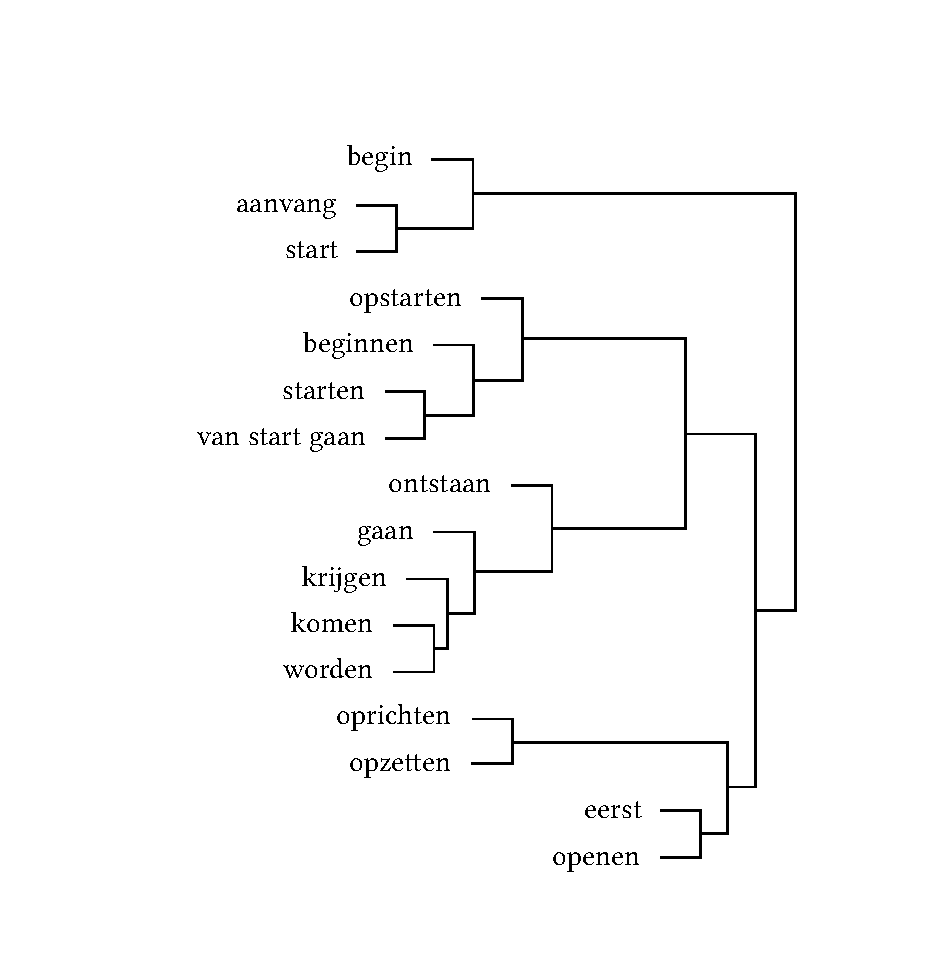
\includegraphics[width=.48\textwidth,trim=95 40 75 75]{figures/tree38.pdf}\hfill%
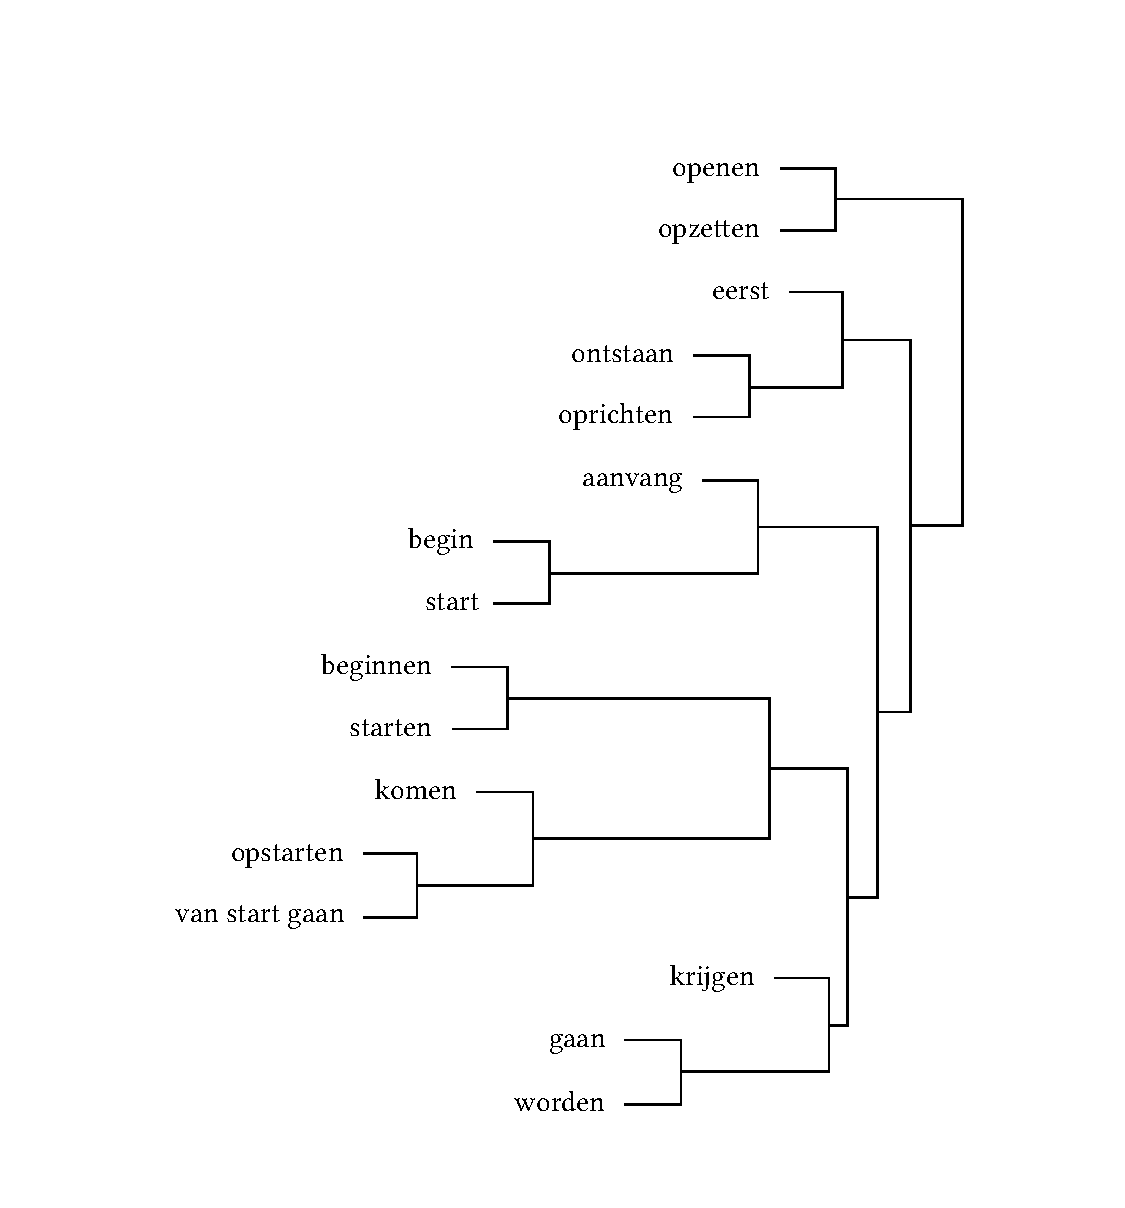
\includegraphics[width=.48\textwidth,trim=95 40 75 75]{figures/tree39.pdf}
\caption{\label{fig:3:38}Left: Euclidean, Ward’s, on LSA (9).\label{fig:3:39}Right: Canberra, Average (10).}
\end{figure}

\begin{figure}
% 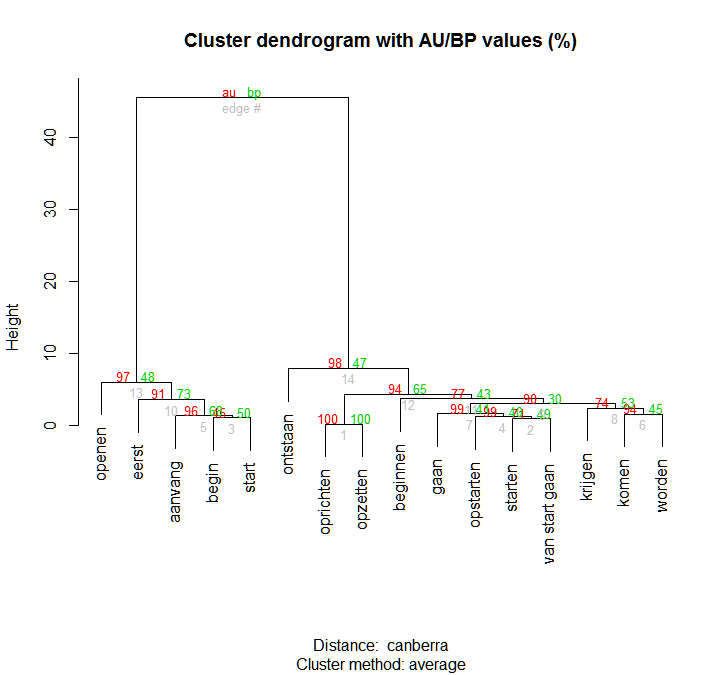
\includegraphics[width=.48\textwidth,trim=95 40 75 75]{figures/Vandevoorde2-img40.png}
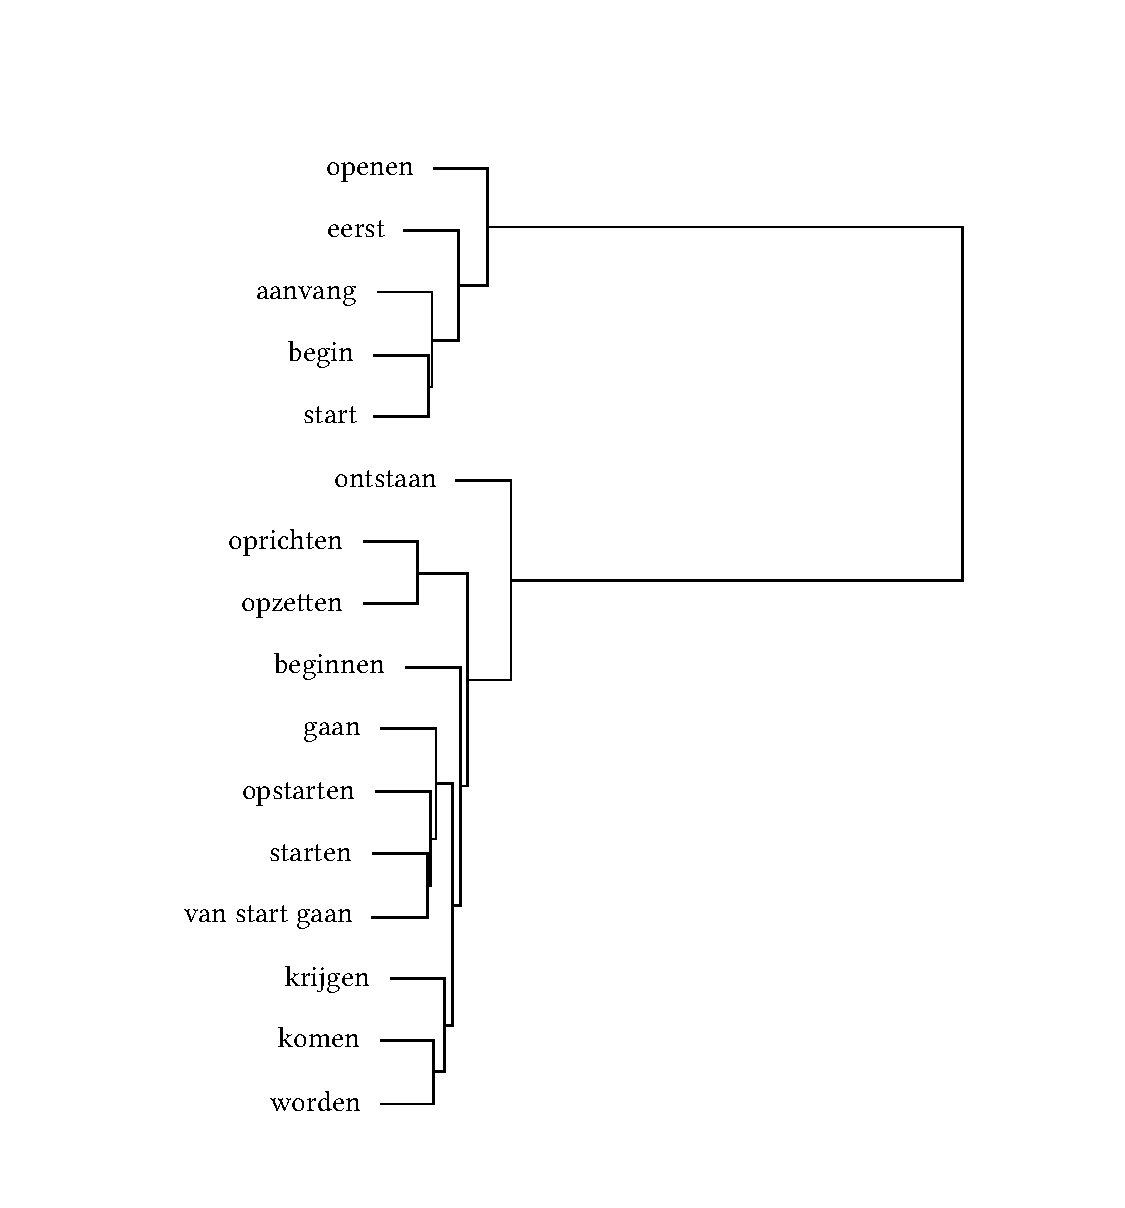
\includegraphics[width=.48\textwidth,trim=95 40 75 75]{figures/tree40.pdf}\hfill%
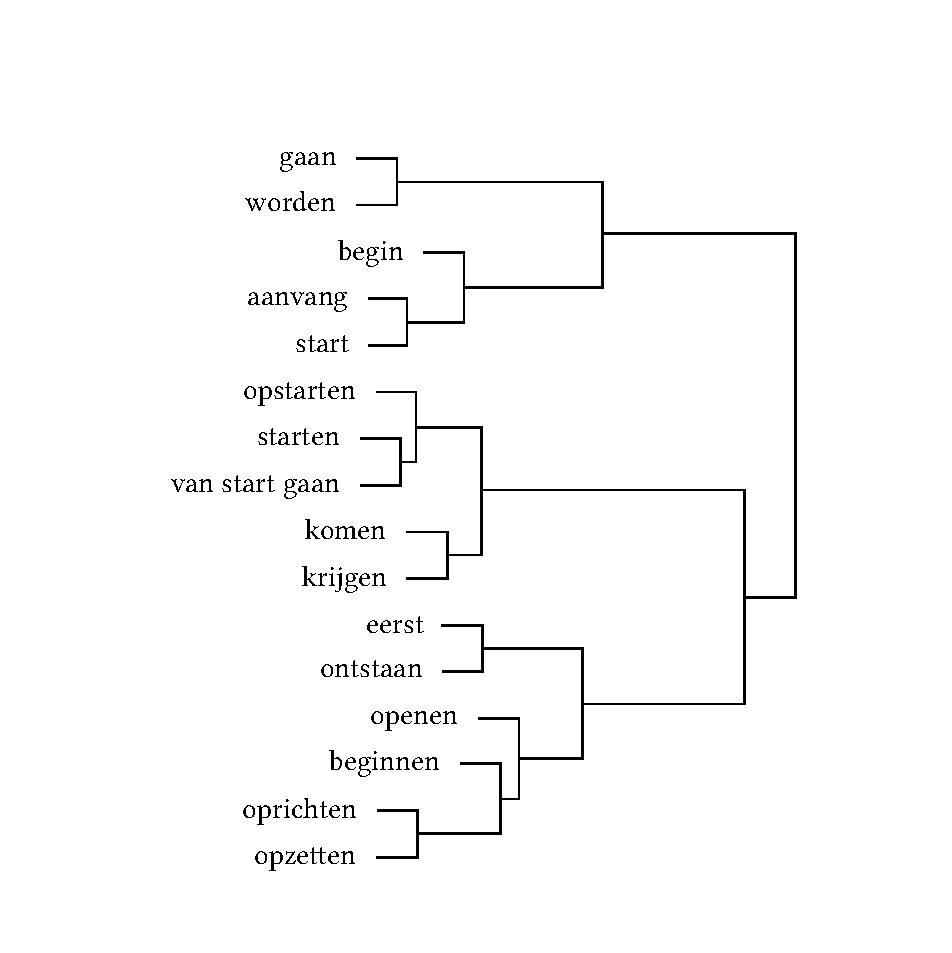
\includegraphics[width=.48\textwidth,trim=95 40 75 75]{figures/tree41.pdf}
\caption{\label{fig:3:40}Left:  Canberra, Average, on CA (11). Right:\label{fig:3:41} Canberra, Average, on LSA (12).}
\end{figure}

\begin{figure}
% 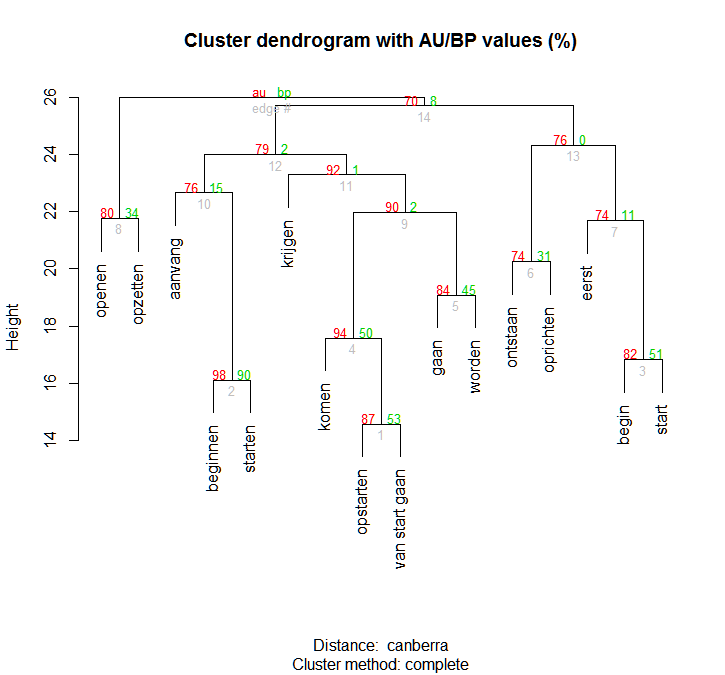
\includegraphics[width=.48\textwidth,trim=95 40 75 75]{figures/Vandevoorde2-img42.png}
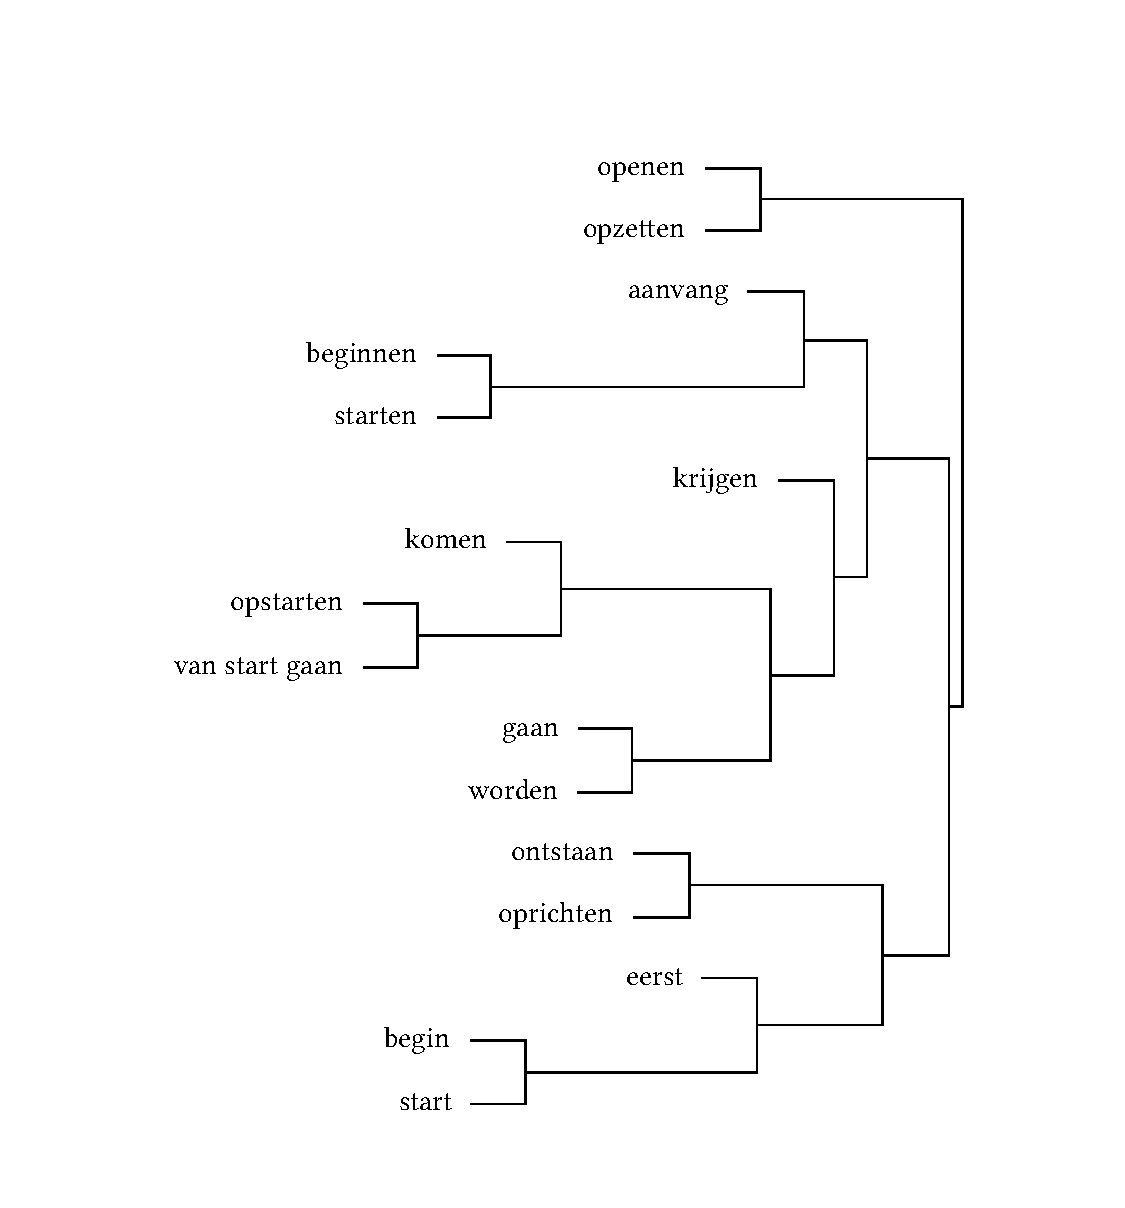
\includegraphics[width=.48\textwidth,trim=95 40 75 75]{figures/tree42.pdf}\hfill%
\includegraphics[width=.48\textwidth,trim=95 40 75 75]{figures/tree43.pdf}
\caption{Left:\label{fig:3:42} Canberra, Complete (13).\label{fig:3:43}Right: Canberra, Complete, on CA (14).}
\end{figure}

\begin{figure}
% \includegraphics[width=.48\textwidth,trim=95 40 75 75]{figures/Vandevoorde2-img44.png}
\includegraphics[width=.48\textwidth,trim=95 40 75 75]{figures/tree44.pdf}\hfill%
\includegraphics[width=.48\textwidth,trim=95 40 75 75]{figures/tree45.pdf}
\caption{\label{fig:3:44}Left: Canberra, Complete, on LSA (15). Right:\label{fig:3:45} Canberra, Ward’s (16).}
\end{figure}

\begin{figure}
% \includegraphics[width=.48\textwidth,trim=95 40 75 75]{figures/Vandevoorde2-img46.png}
\includegraphics[width=.48\textwidth,trim=95 40 75 75]{figures/tree46.pdf}\hfill%
\includegraphics[width=.48\textwidth,trim=95 40 75 75]{figures/tree47.pdf}
\caption{\label{fig:3:46}Left: Canberra, Ward’s, on CA (17). Right:\label{fig:3:47} Canberra, Ward’s, on LSA (18).}
\end{figure}

\clearpage
\section{Statistical approaches to universals on the semantic level}
\label{sec:3.8}
In the previous section \sectref{sec:3.7}, I explained the different decisions that led me to choose HAC carried out on CA to visualize the semantic fields of translated and non-translated inchoativity in Dutch. This methodological development is my answer to the first research question “how to investigate semantic differences?”. In \chapref{sec:4}, the technique developed in the current chapter will be applied to the field of inchoativity in Dutch. In this way, the second research question: “are there any differences on the semantic level between translated and non-translated language?” will be answered, although of course limited to the differences between translated and non-translated Dutch within the field of inchoativity. However, before the results of the case study can be presented in \chapref{sec:4}, more theoretical reflection is needed with respect to the third research question: “if there are any differences between the fields of translated and non-translated Dutch inchoativity, can we ascribe them to any of the universal tendencies of translation?”. In the sub-sections \sectref{sec:3.8.1} and \sectref{sec:3.8.2} below, I will make a number of methodological and conceptual propositions that will enable me to investigate whether the presumed differences between translated and non-translated Dutch on the semantic level might be ascribed to the following universal tendencies: levelling out – which has received very few attention from CBTS researchers (see \sectref{sec:2.2.2.4}) – or normalization and shining through – which take into account specific source and specific target language influence on translated language (see \sectref{sec:2.2.2.3}). For each of these universal tendencies, a difference will be furthermore made between the semasiological and the onomasiological perspective (see \sectref{sec:3.2}), leading to different operationalizations for comparison on the semantic level.

\subsection{Measuring prototypicality effects as a proxy for levelling out}
\label{sec:3.8.1}
Levelling out can be investigated by comparing the variation of a certain feature in translated language to the variation of the same feature in non-translated language (see \sectref{sec:2.2.2.4}). On the semantic level, levelling out can be examined on the semasiological level by comparing the variation of the feature \textit{meaning} \textit{distinctions} in translated language to its variation in non-translated language. For this particular case study, appearance of semantic levelling out on the semasiological level would imply that in translated language, \textit{beginnen} displays fewer meaning distinctions compared to non-translated language. Semantic levelling out could also be investigated on the onomasiological level by comparing the variation of the feature \textit{number} \textit{of} \textit{lexical} \textit{expressions} \textit{per} \textit{meaning} \textit{distinction} in translated language to its variation in non-translated language. For \textit{beginnen,} semantic levelling out on the onomasiological level would manifest itself through the use of fewer lexical expressions to express the different meanings of \textit{beginnen}.

Under the assumption that the meaning distinctions for \textit{beginnen} will be very subtle, I expect that the semantic variation between the fields of translated and non-translated Dutch inchoativity will be small and hence difficult to observe by mere inspection of the clusters in the dendrograms since these clusters are all on an equal par, i.e. they simply represent a partitioning of the lexemes. As a solution to this, I will measure the centrality of each of the meanings (represented as clusters) and focus on possible changes within their prototype-based organization. By determining which clusters are more central in the semantic space and which ones are more peripheral, changes in the prototype-based organization of the meanings within the semantic fields are assessed. Semasiological levelling out will consequently be investigated by looking at the prototype-based organization of the clusters within each dendrogram (SourceDutch, TransDutch\textsubscript{ENG} and TransDutch\textsubscript{FR}). This will be done by comparing the distances-to-centroids of the clusters within each dendrogram (\sectref{sec:3.8.1.1}). Onomasiological levelling out will be investigated by comparing the prototype-based organization of the lexemes in each cluster and for each field (SourceDutch, TransDutch\textsubscript{ENG} and TransDutch\textsubscript{FR}) to each other. This will be done by evaluating the distance of each lexeme to the centroid (considered as the abstract prototype) of the cluster (the meaning distinction) it belongs to (\sectref{sec:3.8.1.2}).

In \sectref{sec:3.8.1.3} I will further explore how centroids and medoids may represent different views on prototypes. In addition, each cluster in a dendrogram will also receive a meta-label as a solution to capture the specific meaning distinction of each cluster (\sectref{sec:3.8.1.4}).

\subsubsection{Organization of clusters within each dendrogram}
\label{sec:3.8.1.1}  
The prototype-based organization of the clusters within each dendrogram will be explored by assessing the distance of each cluster’s center (its centroid) to the zero-point of the semantic space. Centroids correspond to the average of all points in the cluster \citep[494]{tan_introduction_2006}. They can be calculated on the resulting coordinates of the CA (recall that the output of the CA will be used as input for the HAC). The zero-point or origin of a semantic space corresponds to the weighted mean of the columns and of the rows (they are superposed and calibrated on the zero-point). If a data point is situated close to the origin, this implies that its weighted mean is close to the overall weighted mean. The data point can hence be considered as ``central'' in the spatial map, and its profile will be rather resembling to other, equally central points in the spatial map. If Lakoffs idea (\citeyear{lakoff_women_1987}, cited by \citealt{tyler_semantics_2003}) that lexical categories and polysemy networks are structured with respect to their prototypical meanings is accepted, and if Dyvik’s\ia{Dyvik, Helge@Dyvik, Helge} basic idea that “semantically closely related words ought to have strongly overlapping sets of translations” is equally accepted, from which it follows that strongly overlapping sets of translation ought to reveal semantic relatedness, then this leads to the assumption that the central sphere of a spatial map – close to the zero-point or origin – can be considered as the prototypical center. As a consequence, the data points (be it centroids or lexemes) which find themselves in or close to this central sphere can then be considered as prototypical points in the semantic space. The distances of the clusters’ centroids to the zero-point (the prototypical center) of the semantic space they belong to can be informative about the more prototypical or more peripheral position of each cluster (meaning distinction) in the semantic space (the semantic field it belongs to).

The coordinates of the cluster center (the centroid) are calculated on the output of the CA (i.e. the coordinates of the CA) with the built-in function \mbox{\texttt{centers\_ca()}} from the \texttt{svs}-package. Next, the Euclidean distance from each centroid to the zero-point of the semantic space is calculated with \mbox{\texttt{dist\_wrt()}}, a helper function from \texttt{svs}. Finally, the distances of the centroids to the origin of the semantic space are visualized with a dot chart. The example in \figref{fig:3:48} shows the distance of each of the clusters in the HAC visualization for SourceDutch to the origin of the semantic space. Since the zero-point of the semantic space is held to be the prototypical center, clusters that are closer to the zero-point of the semantic space are considerd as more prototypical and clusters further away from the zero-point as more peripheral. 

\begin{figure}
\includegraphics[height=.4\textheight]{figures/Vandevoorde2-img48.png}\vspace*{\baselineskip}
\scriptsize
\begin{tabular}{l>{\itshape}l}
\lsptoprule
Cluster 6 & eerst\\
Cluster 5 & krijgen{\normalfont,} komen{\normalfont,} worden\\
Cluster 4 & ontstaan{\normalfont,} openen\\
Cluster 3 & Starten{\normalfont,} van start gaan{\normalfont,} opstarten{\normalfont,} beginnen{\normalfont,} gaan\\
Cluster 2 & aanvang{\normalfont,} begin{\normalfont,} start\\
Cluster 1 & opzetten{\normalfont,} oprichten\\
\lspbottomrule
\end{tabular}
\normalsize
\caption{\label{fig:3:48}Dot chart presenting the distance of the cluster centroids to the zero-point of the semantic space of SourceDutch}
\end{figure}

\subsubsection{Organization of the lexemes within each cluster}
\label{sec:3.8.1.2}
The prototype-based organization of the different items (lexemes) within each cluster can equally be assessed with centroids by measuring the distance of each lexeme to the centroid of the cluster it belongs to. The Euclidean distance from the lexemes to each of the cluster centroids can be calculated with the function \texttt{dist\_wrt\_centers()} from \texttt{svs} and visualized in a dot chart (an example can be found in \figref{fig:3:49}). The distance of the lexemes to the centroid (the average of all points in the cluster) of the cluster they belong to can be used to explore which lexical items are more prototypical expressions of the particular meaning distinction (indicated by the cluster) and which ones are more peripheral. For the example in \figref{fig:3:49}, we see that \textit{starten} and \textit{beginnen} are the lexemes situated closest to the centroid of the cluster they belong to, implying that they are closest to the abstract prototype contained in the centroid.

\begin{figure}
\includegraphics[height=.4\textheight]{figures/Vandevoorde2-img49.png}
\caption{\label{fig:3:49}Dot chart representing the distance of the lexemes to the centroid of cluster n°4 for SourceDutch}
\end{figure}

The stability of the cluster membership of each lexeme can also be determined on the basis of this analysis. HAC is categorized as hard clustering, which means that each object in the analysis can be assigned to only one cluster (in contrast to fuzzy clustering, which can reveal the degree of membership of an object to a cluster). By looking at the distance of the lexemes to their cluster’s centroid, the hard clustering is somewhat nuanced. The positions of the lexemes with respect to their centroid may show that some lexemes are ``hesitant'' between two clusters, and their assignment to a particular cluster is not as straightforward and clear-cut (as hard) as the dendrogram structure would have suggested. The centroid itself, however, is not a meaningful point\footnote{\citet[516]{manning_foundations_1999} point out that the centroid “is in most cases not identical to any of the objects”.} since it is the average of all points. Alternatively, it is possible to compute the medoid for each cluster, which is the particular point in the cluster with the smallest average distance to all other points \citep[164]{divjak_structuring_2010}. Everitt et al. \citep[113]{everitt_cluster_2011} note that the term medoid was coined by \citet{kaufman_finding_1990} by analogy with calling the group mean the centroid. The medoid “can be interpreted as a representative object or exemplar of the group” \citep[113]{everitt_cluster_2011} and is necessarily one object in the cluster; this object can then be considered as the “prototypical class member” \citep[516]{manning_foundations_1999} in a cluster. The medoid can be calculated with the \texttt{pam()}-function in R (``Partitioning around Medoids'').

For each cluster analysis, I will calculate both the medoid of each cluster as well as the distance of each lexeme to the centroid of the cluster it belongs to. Both measures seem to have their own advantage(s). The distances of each of the lexemes to the centroid allow to better understand the organization of the lexemes in a cluster as a ``continuum'' with some lexemes closer to the centroid (the most central ones) and others further away from the centroid (the most peripheral ones). The medoid on the other hand indicates one particular lexeme but is less informative about the structure of the cluster. If the medoid happens to be different from the lexeme closest to the centroid, this could indicate tension between several prototypical expressions.

\subsubsection{Centroids and medoids: Different views on prototype}
\label{sec:3.8.1.3}
Both measures (distance to the centroid and medoid) can be used to determine which lexical item in each cluster can be considered as the most prototypical expression of that cluster (the particular meaning distinction indicated by the cluster). However, distance to centroid and medoid could be seen as representing two different views on prototypes.

Descriptions of the prototype-based organization of the lexical items in a cluster which rely on the distance of the items to the centroid imply that prototype is regarded as a “summary representation” \citep[42]{murphy_big_2004}, meaning that “an entire category is represented by a unified representation” where “[t]he concept is represented as features that are usually found in the category members, but some features are more important than others” \citep[42]{murphy_big_2004}. Because such a summary representation is (always) abstract, it would strictu sensu not be possible to capture the summary representation within only one lexeme of the cluster (since the prototype would be an abstract sum of features). However, it is also possible to consider the lexeme closest to the centroid as the one that – in the best way possible – reunites the features usually found in the category members, without considering it as the ``ideal member'' (the ideal member would be the centroid itself, which does not coincide with any of the cluster’s members). Hence, the lexeme closest to the centroid can be seen as the best possible representation of the abstract prototype contained in the centroid. If the medoid of a cluster is regarded as the prototype of the cluster it belongs to (the particular meaning distinction), this would correspond to Murphy’s “best example idea” \citep[42]{murphy_big_2004}, where “a single prototype could represent a whole category” \citep[42]{murphy_big_2004}. The medoid then indicates the best example as the prototype of the cluster it belongs to.

\subsubsection{Manual assignment of meta-labels}
\label{sec:3.8.1.4}  

A meta-label will be assigned to each cluster in the dendrogram in an effort to name the specific meaning distinction indicated by the cluster. There are several options to arrive at such a label. Firstly, either the lexeme closest to the centroid or the medoid of each cluster can be selected as its meta-label. However, since only 16 lexemes will be making up the dendrograms, several small clusters are to be expected (with 3 or fewer members). Indicating one of the few lexemes in such a small cluster as its meta-label will most likely not have much informative value with respect to the specific meaning distinction of that cluster.

Secondly, other quantitative techniques can be applied in an attempt to provide supplementary information about each cluster. This would, however, require an expansion of the amount and nature of annotated data in the data sets. It is possible, for instance, to carry out a supplementary annotation (e.g. of contextual information) and to add this information to the analysis. One possibility would be to apply a behavioral profiling \citep{divjak_ways_2006, divjak_clusters_2008, evans_behavioral_2009} to the resulting data sets (which would consist in coding each item occurring in each of the sentences for a number of variables, known as ID tags).\footnote{While such an analysis would have certainly yielded new insights, it could not be carried out within the scope of this study.} A third option is to manually label each cluster in an attempt to capture its specific meaning distinction via a more qualitative analysis of each cluster. For this study, I will opt for such a manual assignment task, which will consist in a thorough inspection of each cluster in a dendrogram. The assigned meta-label will combine information of three types of sources: corpus examples from the DPC containing the lexemes which make up a cluster, attestations in reference works and information from the lexical database Cornetto \citep{vossen_cornetto_2008, spyns_cornetto:_2013}. Cornetto is a lexical data base for Dutch which consists of two existing semantic resources (Dutch Word Net and Referentiebestand Nederlands). It was created within the same project (STEVIN) as the Dutch Parallel Corpus that we are using in this study (see \sectref{sec:3.3}). The semantic properties of words are described in Cornetto by the categories Sentiment (with labels such as ``positive'' and ``negative''), Pragmatics (including usage information about domain, chronology, connotation, geography and register), Semantics (with specific values for each part-of-speech) and SenseExamples (information about the combinatoric properties). The integration of the variety of semantics-related information obtained via Cornetto could also have been done in a quantitatively more robust way, rather than via the qualitative analysis I propose.\footnote{A quantitatively more robust way of integrating this variety of informative semantics-related labels into the analysis would be to manually tag the resulting data sets of the SMM++ with the semantic information from Cornetto and carry out an analysis using those tags as variables (as an alternative analysis to the clustering on the basis of translations\slash source language lexemes). Another option would be to add the information of these semantics-related labels as supplementary points to a Correspondence Analysis based on the translational data. Thirdly, one could also envisage to use the previously obtained translational information as an additional tag and carry out a cluster analysis using both the semantics-related labels and the translations as variables.} However, such an operation would have (again) required an expansion of the amount and nature of annotated data (the resulting data sets of the SMM++ would need supplementary annotation with the semantic information from Cornetto before an analysis using those tags as variables could be carried out). Although such an analysis would definitely enrich the dendrograms and consequently allow for more fine-grained descriptions of the clusters – while simultaneously adding interpretative power – I did not further investigate this option within the purview of this study, mainly because the main focus of this book is to explore as many potentialities as possible of translational data ``alone'' for semantic description, without using any additional annotative information in the analysis.

\subsection{Semantic fields of \textit{commencer} and \textit{to begin}}
\label{sec:3.8.2}  
The investigation of semantic normalization and shining through on both the semasiological and the onomasiological level requires a number of additional visualizations.

On the semasiological level, target language influence on the meaning distinctions in translated Dutch inchoativity (\textsc{semasiological normalization}) will be investigated by comparing the meaning distinctions in translated Dutch to those present in non-translated Dutch. Source language influence on the meaning distinctions in translated Dutch inchoativity (\textsc{semasiological shining through}) will be investigated by comparing the meaning distinctions in translated Dutch to those present in the source languages. This will be done by visualizing the semantic fields of the closest equivalents of \textit{beginnen} in the source languages of TransDutch\textsubscript{ENG} and TransDutch\textsubscript{FR}, viz. SourceEnglish \textit{to} \textit{begin} and SourceFrench \textit{commence}r. The meaning distinctions in the fields of \textit{to} \textit{begin} and \textit{commencer} are compared to those present in TransDutch\textsubscript{ENG} and TransDutch\textsubscript{FR} respectively, to see whether the specific meaning distinctions within the semantic fields of SourceEnglish and SourceFrench might have influenced the organization of the meaning distinctions in TransDutch\textsubscript{ENG} and TransDutch\textsubscript{FR}. The resulting semantic spaces of inchoativity in French and English are independent of TransDutch and correspond to the second T-images\footnote{Note that for \textit{commencer} and \textit{to} \textit{begin}, only one mirroring can be carried out (i.e. with a single Language B – Dutch) since the DPC does not contain the translation directions French-English, English-French. Consequently, the data sets for the \textit{second} \textit{T-images} are based on a single data set (compared to the second T-image data set for SourceDutch, which consists of the combined data of the second T-image of \textit{beginnen}\textsubscript{FR} and \textit{beginnen}\textsubscript{ENG}).} of \textit{commencer} and of \textit{to} \textit{begin.}

With \textsc{onomasiological normalization}, I refer to the possible influence of non-translated Dutch on the prototype-based organization of the lexemes within each meaning distinction of \textit{beginnen} in translated Dutch. This can be assessed by comparing the prototype-based organization of the lexemes in each meaning distinction in SourceDutch to the organization of the lexemes in each meaning distinction in TransDutch\textsubscript{ENG} and TransDutch\textsubscript{FR}. If the same organization of lexemes appears in TransDutch\textsubscript{ENG} and TransDutch\textsubscript{FR} and this organization is similar or identical to the organization in SourceDutch, there is a good chance that the TransDutch fields are ``conforming'' to the SourceDutch field, yielding evidence for onomasiological normalization. \textsc{Onomasiological shining through} would manifest itself as an influence of the source language on the organization of the lexemes within each meaning distinction of \textit{beginnen} in translated Dutch. In order to asses such an influence, the English and French source language lexemes – which determine the clustering of the Dutch lexemes in TransDutch\textsubscript{ENG} and TransDutch\textsubscript{FR} into specific meaning distinctions – will be visualized together with the Dutch target language lexemes. In this way, it can be observed how the specific organization of the lexical items within the clusters – with each cluster representing a particular meaning distinction of \textit{beginnen} – is possibly influenced by a specific underlying source language lexeme. In order to obtain a simultaneous representation of the source and target language lexemes in a single semantic space, I will carry out a Multiple Correspondence Analysis on a Burt table \citep{greenacre_simple_2006, greenacre_correspondence_2007}. Burt Tables are generalizations of ordinary frequency tables with row and column categories, in that they cross all categories as rows with all categories as columns. The advantage of a Multiple Correspondence Analysis on a Burt table is that distances can be computed, not only between (Dutch) target lexemes themselves, but also between target lexemes and source lexemes so that both source language lexemes and target language lexemes are represented in a single space. This MCA on a Burt table is subsequently visualized with a HAC, enabling us to visually inspect which Dutch target lexemes are associated with which French or English source lexemes.

\section{Conclusion}
\label{sec:3.9}  
In this chapter, I have proposed a methodology to investigate semantic differences between translated and non-translated language. The method is an extension of an existing method (the SMM); it is corpus-based, uses statistical visualization techniques and consists of two parts (two extensions to the SMM). The first extension allows the potential user of the method to select candidate-lexemes for a semantic field. This selection mechanism (retrieval method) is translation-driven and uses the different translational statuses (either source or target language) of parallel corpus data. The second extension to the SMM proposes a way to visually inspect the retrieved data sets via a combination of CA and HCA. First, CA is applied in order to construct a low-dimensional semantic space of the data. Second, HAC is applied in order to distinguish clusters of lexemes within the semantic spaces. The technique is calibrated by the Euclidean distance measure and Ward’s Minimum Variance Method as the amalgamation rule. In this methodological chapter, the way was furthermore paved to investigate levelling out, shining through and normalization on both the semasiological and the onomasiological level.

In the next chapter, I will apply the two extensions of the SMM to the semantic field of inchoativity in Dutch. The comparison of different visualizations representing the semantic fields of SourceDutch, TransDutch\textsubscript{ENG} and TransDutch\textsubscript{FR} will enable me to tackle the second question I aim to answer with this study: “Are there any of the (universal) tendencies of translation that also apply to the semantic level?” as well as the third one: “If there are differences on the semantic level, can we ascribe them to any of the (universal) tendencies of translation?”.
 
\chapter{Results}
\label{sec:4}
\section{Introduction}
\label{sec:4.1}  
The outline of this chapter is as follows: in \sectref{sec:4.2}, \sectref{sec:4.3} and \sectref{sec:4.4}, I will provide a description as well as an interpretation of the visualizations of the semantic field of \textit{beginnen}/inchoativity of SourceDutch, TransDutch\textsubscript{ENG} and TransDutch\textsubscript{FR} respectively, yielded on the basis of the methodological procedure developed in the previous chapter. Each description will consist of the following elements: (i) the results of the Hierarchical Agglomerative Cluster Analysis (carried out on the output of a Correspondence Analysis), (ii) a description of the prototype-based organization of the clusters in the dendrogram based on the distances of the centroids to the zero-point of the semantic space, (iii) a description of the prototype-based organization of the lexemes within each cluster based on the distances of the lexemes in each cluster to their cluster’s centroid , (iv) a description of the medoid of each cluster. The distances of the centroids to the zero-point of the semantic space (the prototypical center) inform us on the semasiological level about the prototype-based organization of the clusters (the meaning distinctions) in the semantic space (the semantic field of \textit{beginnen}). The distances of the lexemes to the centroid of the cluster give us more information on the onomasiological level about the prototype-based organization of the lexemes within each cluster. The medoid (the best exemplar) as well as the lexeme closest to the centroid of a cluster (the best representation of the abstract prototype) can be used to determine the most prototypical expression in each cluster. Finally, (v) an in-depth interpretation of each visualization representing a semantic field of \textit{beginnen}/inchoativity will be provided, on the basis of which a meta-label will be determined for each cluster so as to name the specific meaning distinction revealed by that cluster. The meta-labels that I will assign should be understood as a post-hoc, interpretative tool, applied to enhance my understanding of the rendered dendrograms. It should be clear that my attempt to present such a post-hoc interpretation of the quantitative and statistical information in terms of semantic change needs to be seen as a first exploration of the field of inchoativity and by no means an endpoint. In \sectref{sec:4.5}, \sectref{sec:4.6} and \sectref{sec:4.7} I will present my insights with respect to tendencies of levelling out, shining through and normalization each time on both the semasiological and the onomasiological level. The interpretations of the fields of SourceDutch, TransDutch\textsubscript{ENG} and TransDutch\textsubscript{FR} described in the previous sections will be used as a basis here. Statements about semasiological change will be based on the outcome of a statistical analysis and an interpretation of clusters as meaning distinctions. Conclusions about onomasiological change will be based on measurements of minimal (and hence subtle) differences in distances to an abstract prototype contained in the centroid. 

\section{SourceDutch}
\label{sec:4.2}  
\subsection{Results of the Hierarchical Agglomerative Cluster analysis}
\label{sec:4.2.1}  
Following the procedure described in \chapref{sec:3}, I carried out a HAC on the output of a CA. I first applied the statistical technique of CA. The scree plots in Figures 50 and 51 show the distribution of the variation over the latent dimensions of the CA. The cumulative scree plot (\figref{fig:4:51}) shows that at least 5 dimensions are needed to represent more than 80\% of the variation:

\begin{figure}
\includegraphics[height=.4\textheight]{figures/Vandevoorde2-img50.png}
\caption{\label{fig:4:50}  Scree plot for SourceDutch}
\end{figure}

\begin{figure}
\includegraphics[height=.4\textheight]{figures/Vandevoorde2-img51.png}
\caption{\label{fig:4:51}  Cumulative scree plot for SourceDutch}
\end{figure}

On the basis of this scree plot, I reduced the number of dimensions of the CA to 5. This step is important to avoid noisy (less informative) data patterns. A HAC was then carried out on the output of the CA. The cut-off point was set at a height of 4 (following the rationale described in \chapref{sec:3}),\footnote{Note that with \texttt{pvrect()}, which cuts off each cluster at the highest possible node with a significant p\textsuperscript{{}-}value – the same cluster solution would have been obtained.} resulting in a cluster solution with 6 clusters: cluster n°1 contains \textit{oprichten} [to establish] and \textit{opzetten} [to set up]; cluster n°2 includes \textit{aanvang} [commencement], \textit{begin} [beginning] and \textit{start} [start]; cluster n°3 comprises \textit{opstarten} [to start up], \textit{starten} [to start], \textit{van} \textit{start} \textit{gaan} [to take off], \textit{beginnen} [to begin] and \textit{gaan} [to go]; cluster n°4 holds \textit{ontstaan} [to come into being] and \textit{openen} [to open]; cluster n°5 consists of \textit{komen} [to come], \textit{krijgen} [to get] and \textit{worden} [to become]; cluster n°6 contains \textit{eerst} [firstly]. I consider the result presented in \figref{fig:4:52} as a possible visualization of a semantic field of \textit{beginnen}/inchoativity in SourceDutch.

\begin{figure}  
% \includegraphics[height=.4\textheight]{figures/Vandevoorde2-img52.png}
\includegraphics[width=\textwidth]{figures/tree52.pdf}
\caption{\label{fig:4:52}  Dendrogram representing a semantic field of \textit{beginnen}/inchoativity for SourceDutch}
\end{figure}

In order to validate the chosen cluster solution with 6 clusters, I calculated the average silhouette width. I obtained an average silhouette width of 0.59 for this cluster solution, which is above the 0.50 threshold for good classification determined by Kaufman and Rousseeuw (see \sectref{sec:3.7.2.3}).

\begin{figure}
\includegraphics[height=.4\textheight]{figures/Vandevoorde2-img53.png}
\caption{\label{fig:4:53}  Average silhouette width for cluster solution with 6 clusters for SourceDutch}
\end{figure}

A K-means clustering was carried out as a second validation technique for the chosen cluster solution. When a cluster solution with 6 clusters was requested, the K-means clustering shown in Figure 4.5 was proposed (the numeral to the left of each lexeme assigns it to a specific cluster):
  
\begin{figure}
% \includegraphics[width=\textwidth]{figures/Vandevoorde2-img54.png}
\footnotesize
\begin{lstlisting}
Clustering vector:
      aanvang       begin    beginnen      eerst             gaan 
            2           2           3          6                3         
        komen     krijgen    ontstaan     openen        oprichten         
            5           5           4          4                1         
    opstarten    opzetten       start    starten   van start gaan         
            3           1           2          3                3         
       worden                                            
            3                                      
\end{lstlisting}     

\caption{\label{fig:4:54}  K-means clustering with 6 clusters for SourceDutch}
\end{figure}

Note that the only difference with the output of the HAC is that \textit{worden} is assigned to the cluster containing \textit{starten}, \textit{van} \textit{start} \textit{gaan,} \textit{opstarten,} \textit{beginnen}, and \textit{gaan}. On the basis of both validation techniques, I consider my cluster solution for SourceDutch as a good classification. In addition, as a result of the K-means clustering it can be concluded that the clustering of the polyfunctional verb \textit{worden} seems to be uncertain.

\subsection{Prototype-based organization of the clusters in the dendrogram (semasiological level)}
\label{sec:4.2.2}  
In order to obtain more information about the prototype-based organization of the clusters (meaning distinctions) within each dendrogram, I determined the distance of the centroids of each cluster to the origin or zero-point of the semantic space (the prototypical center). The centroids were subsequently mapped onto a dot chart (\figref{fig:4:55}). The cluster closest to the zero-point is considered to be the most central one in the semantic space.

\begin{figure} 
\includegraphics[height=.4\textheight]{figures/Vandevoorde2-img55.png}
\scriptsize
\begin{tabular}{ll}
\lsptoprule
Cluster 6 & eerst\\
Cluster 5 & krijgen, komen, worden\\
Cluster 4 & ontstaan, openen\\
Cluster 3 & Starten, van start gaan, opstarten, beginnen, gaan\\
Cluster 2 & aanvang, begin, start\\
Cluster 1 & opzetten, oprichten\\
\lspbottomrule
\end{tabular}
\normalsize
\caption{\label{fig:4:55}  Dot chart presenting the distance of the cluster centroids to the zero-point of the semantic space of SourceDutch}
\end{figure}

Note that the numerals on the y-axis of the dot chart in \figref{fig:4:55} were assigned by a previously established list (based on the output of the cluster analysis), necessary to calculate the cluster centroids (the order of the assigned numerals is arbitrary). The content of each cluster number is resumed in the table accompanying \figref{fig:4:55}. The dot chart shows us that cluster n°3, containing \textit{starten}, \textit{van} \textit{start} \textit{gaan}, \textit{opstarten}, \textit{beginnen} and \textit{gaan} is the most central cluster in the analysis, rather closely followed by cluster n°2 comprising \textit{aanvang,} \textit{begin} and \textit{start}. Then, clusters n°4 (\textit{ontstaan} and \textit{openen}), n°5 (\textit{komen}, \textit{krijgen} and \textit{worden}), n°6 (\textit{eerst}) and n°1 (\textit{oprichten,} \textit{opzetten)} are situated considerably further away but at an almost equal distance of the plot’s origin.

\subsection{Prototype-based organization of the lexemes within each cluster (onomasiological level)}
\label{sec:4.2.3}  
Next, the prototype-based organization of the lexemes within each cluster was inspected by measuring the distance of the lexemes of each cluster to the centroid of the cluster they belong to. In addition, I calculated the medoid of each cluster. Both the lexeme closest to the centroid and the medoid can be used to determine which lexical item in each cluster can be considered as the most prototypical expression of that cluster although I regard the two measures as different views on prototypes: the lexeme closest to the centroid is considered as the best possible representation of the abstract prototype contained in the centroid, the medoid indicates the best example as the prototype of the cluster it belongs to.

\subsubsection{Centroids}
\label{sec:4.2.3.1}  
Each of the six dot charts (Figures 56 to 61) represents one of the six clusters of SourceDutch. The centroid of the represented cluster is taken as the zero-point of the dot chart, so that the lexemes pertaining to this cluster are the closest ones to the zero-point of the dot chart. This allows me to visualize which lexemes are more central, and which ones more peripheral in the cluster. In addition, these visualizations also show the distance of the lexemes of all the other clusters to the represented cluster centroid. This is especially interesting for lexemes of which the proposed clustering on the basis of the HAC appeared uncertain (e.g. \textit{worden}).

\begin{figure}
\includegraphics[height=.4\textheight]{figures/Vandevoorde2-img56.png}
\caption{\label{fig:4:56}  Cluster n°1 for SourceDutch}
\end{figure}

\begin{figure}
\includegraphics[height=.4\textheight]{figures/Vandevoorde2-img57.png}
\caption{\label{fig:4:57}  Cluster n°2 for SourceDutch}
\end{figure}

\begin{figure}
\includegraphics[height=.4\textheight]{figures/Vandevoorde2-img58.png}
\caption{\label{fig:4:58}  Cluster n°3 for SourceDutch}
\end{figure}

\begin{figure}
\includegraphics[height=.4\textheight]{figures/Vandevoorde2-img59.png}
\caption{\label{fig:4:59}  Cluster n°4 for SourceDutch}
\end{figure}

\begin{figure}
\includegraphics[height=.4\textheight]{figures/Vandevoorde2-img60.png}
\caption{\label{fig:4:60}  Cluster n°5 for SourceDutch}
\end{figure}

\begin{figure}
\includegraphics[height=.4\textheight]{figures/Vandevoorde2-img61.png}
\caption{\label{fig:4:61a}  Cluster n°6 for SourceDutch}
\end{figure}


Since the difference in distance of the members of a same cluster to their cluster’s centroid is often minimal, I used the calculated distances (which are represented by the dots in the dot charts) to evaluate the distances to the centroids (see \tabref{appendix-table-H}, Appendix~\ref{ch:C}).

For cluster n°1, the distance from \textit{opzetten} to the centroid is 0.06749455, whereas the distance from \textit{oprichten} to the centroid is 0.02952887, implying that \textit{oprichten} is closer to the centroid, and can thus be considered as the best representation of the abstract prototype of cluster n°1. For cluster n°2, the distance from \textit{start} to the centroid is 0.20740218 and the distance from \textit{begin} to the centroid is 0.08908994. This shows that \textit{begin} is closer to the centroid and can be considered as the best representation of the abstract prototype of cluster n°2. For cluster n°3, four lexemes are very close to the zero point. \textit{Van} \textit{start} \textit{gaan,} \textit{gaan} and \textit{opstarten} are slightly further away from the cluster’s centroid, but the difference in distance between \textit{starten} and \textit{beginnen} is minimal. The distance from \textit{starten} to the centroid is 0.1264550, and the distance from \textit{beginnen} to the centroid is 0.1254173. Hence, \textit{beginnen} is indicated as the cluster’s best representation of the abstraction of the prototype. With regard to cluster n°4, \figref{fig:4:59} clearly shows that \textit{openen} is the closest lexeme to the centroid, and can hence be considered as the best representation of the abstract prototype of this cluster. As for cluster n°5, \textit{komen} can clearly be distinguished as the closest lexeme to the centroid, and is indicated as its best representation of the abstract prototype. Finally, it is unnecessary to indicate the best representation of the abstract prototype for cluster n°6, which is a singleton cluster with \textit{eerst}.

\subsubsection{Medoids}
\label{sec:4.2.3.2}  
A second quantitative possibility to obtain more information about the organization of the lexemes within each cluster is to calculate its medoid. The medoid assigns one object in the cluster from which the average distance to all other objects is the smallest \citep[164]{divjak_structuring_2010}. The medoids for the clusters are summarized in \tabref{tab:4:14} and compared to the lexeme closest to the centroid as determined above. The table shows that the medoid and the lexeme closest to the centroid never converge (clusters n°1, 4 and 6 are disregarded since they have only one or two members):

\begin{table}
\caption{\label{tab:4:14}  Comparison of medoids and lexemes closest to the centroids for SourceDutch}
\begin{tabularx}{\textwidth}{XXl} 
\lsptoprule
Cluster & Medoid & Lexeme closest to centroids\\
\midrule
Cluster n°2 & Start & Begin\\
Cluster n°3 & Starten & Beginnen\\
Cluster n°5 & Krijgen & Komen\\
\lspbottomrule
\end{tabularx}
\end{table}

The divergence between the closest lexeme to the centroid and the medoid of a cluster for all clusters increases the uncertainty about which lexeme can be considered as the most central one. In addition, the difference in distance to the centroid is minimal for some clusters, especially for cluster n°3 (\textit{beginnen} vs.\ \textit{starten}) and cluster n°2 (\textit{begin} vs.\ \textit{start}). It is noteworthy that for those two clusters with a minimal difference in distance to the centroid, it is the second closest lexeme that is indicated as the medoid each time. This is potentially very interesting and could indicate a field of tension between several of the more central expressions in each cluster.

The diverging evidence from medoids and distance to centroids makes it difficult to put forward the outcome of the one or the other measure as the better one to determine the most prototypical expression for each cluster, all the more because they have been linked to different views on prototype. As a consequence, neither the lexeme closest to the centroid nor the medoid will be used as a meta-label to name the specific meaning distinction of the cluster.

\subsection{Interpretation of the semantic field of \textit{beginnen}\slash inchoativity for SourceDutch}
\label{sec:4.2.4}  
I will now provide an interpretation of the visualization representing a semantic field of \textit{beginnen}/inchoativity for SourceDutch.\footnote{Substantial parts of the interpretations of the visualizations of SourceDutch, TransDutch\textsubscript{ENG} and TransDutch\textsubscript{FR} in \sectref{sec:4.2.4} \sectref{sec:4.3.4} and \sectref{sec:4.4.4} of this book have been first presented in \citep{vandevoorde_corpus-based_2017}, an article which is under copyright. Its publisher should be contacted for permission to re-use or reprint the material in any form.} This interpretation will be used to determine a meta-label for each cluster so as to name the specific meaning distinction revealed by that cluster. The meta-labels that I will assign should be understood as a post-hoc, interpretative tool, applied to enhance my understanding of the rendered dendrograms. Note that I do not consider the meta-labels as a validation of the discerned cluster organization – if this had been my intention, I should have determined the labels beforehand. As determined in \sectref{sec:3.8.1.4}, information from three types of sources will be used (in addition to the information about the prototype-based organization of the clusters in the field and the lexemes in each cluster): (i) corpus examples from the DPC containing the lexemes which make up a cluster (ii) attestations in reference works and (iii) information from the lexical database Cornetto \citep{vossen_cornetto_2008, spyns_cornetto:_2013}. 

I consider cluster n°3 as the most central cluster or \textsc{reference cluster}, representing the idea of \textsc{general onset}. There are two arguments to justify this. First, on the semasiological level this cluster’s centroid is the closest one to the origin of the semantic space and hence, the most central one in the prototype-based organization of the semantic field. Second, on the onomasiological level, Figures 56 to 61 – which depict the distances of the lexemes to each of the centroids of the other clusters – show that the lexemes of cluster n°3 are always situated at a fairly equal distance of the centroids of all the other clusters (somewhat in the middle of each plot). This implies that cluster n°3 shows the least deviation with respect to the other clusters (the lexemes of cluster n°3 are all equally similar to the abstract prototype of each of the other clusters). Third, cluster n°3 holds the initial lexeme \textit{beginnen}, which was selected to initiate the SMM++ retrieval task since it is considered as the most prototypical expression of inchoativity (based on corpus frequency and etymological age). The cluster containing \textit{beginnen} is believed to hold the most prototypical expressions of inchoativity.

Cluster n°3 contains three different sub-nodes, one with \textit{opstarten} [to start up], and two other, interrelated sub-nodes; one with \textit{starten} [to start] and \textit{van} \textit{start} \textit{gaan} [to take off] and another one with \textit{beginnen} [to begin] and \textit{gaan} [to go]. In my opinion, these latter two interrelated sub-nodes indicate an additional meaning-distinction within the meaning-distinction indicated by cluster n°3. Besides \textit{beginnen}, \textit{starten} is also a typical expression of inchoativity, and the two are often considered as near-synonyms \citep[223]{schmid_introspection_1996}. \citet{lewandowska-tomasczyk_corpus-based_2009} – based on research by \citet{biber_longman_1999} and \citet{schmid_cottage_1993}, following \citet{quirk_comprehensive_1985} – conclude the following for the English phasal verbs \textit{to} \textit{start} and \textit{to} \textit{begin}:

\begin{quote}
\textbf{Begin} then gives a view into the state after onset of the action: it expresses modality\slash intentionality and refers to \textbf{later} \textbf{states} \textbf{of} \textbf{affairs}. It typically applies to cognitive-emotive events and non-perceivable things. \textbf{Start}, on the other hand, focuses on the \textbf{actual} \textbf{action}, the actual beginning, the very moment of transition from non-action to action. It is dynamic and applies to visible change and actions (\citealt[279]{lewandowska-tomasczyk_corpus-based_2009}, my emphasis).
\end{quote}

The subdivision observed in the (Dutch) results into verbs formally related to \textit{starten} [to start] such as \textit{van} \textit{start} \textit{gaan} [to take off] on the one hand (hence: \textsc{action} verbs), and verbs formally related to \textit{beginnen} [to begin] (hence: \textsc{state after onset} verbs) on the other hand, corroborates the distinction made by Divjak \& Gries. The attested distinction between \textit{to} \textit{start} and \textit{to} \textit{begin} seems to hold for Dutch \textit{starten} and \textit{beginnen}, too. Recall that the two lexemes closest to the centroid of this cluster are indeed \textit{beginnen} (0.1254173) and \textit{starten} (0.1264550); the minimal difference in distance to the centroid between these two lexemes further shows that there is some kind of ``competition'' going on between the two and that either of the two would be a good candidate to be the best representation of the abstract concept of the prototype. Further note that the distinction between \textsc{action} and \textsc{state after onset} is not indicated in Cornetto, which classifies all the lexemes of cluster n°3 as the same semantic type, i.e. action (“verb that describes an action that is usually controlled by the subject of the verb”), with the only exception that \textit{beginnen} can also be granted the semantic type process (“a dynamic event that is not initiated by an actor capable of acting with volition”). According to the lexical-semantic database Cornetto \citep{vossen_cornetto_2008}, \textit{gaan} [to go],\footnote{Recall that observations of \textit{gaan} in the construction \textit{van} \textit{start} \textit{gaan} are not included here.} which somewhat oddly seems to be clustered with \textit{beginnen}, is defined as “beginnen iets te doen” [to begin to do something], and \textit{beginnen} as “iets gaan doen” [to go and do something]. The definitional relation indicated by Cornetto seems to underpin the semantic relationship indicated by the clustering of \textit{beginnen} and \textit{gaan}. In addition, according to the Algemene Nederlandse Spraakkunst (General Dutch Grammar) \citep{haeseryn_algemene_2012}, the first of two subtypes of \textit{gaan} “without the meaning of motion” is the subtype where \textit{gaan} has the meaning of “‘(geleidelijk) overgaan tot’, ‘beginnen te’ (inchoatief aspect)” [(gradually) move on to, to begin to (inchoative aspect)]. The relatedness between \textit{starten} and \textit{beginnen} is also further substantiated by the definitions of \textit{starten} in Cornetto: (i) “beginnen van iets (niet-causatief)” [beginning of something (non-causative)], (ii) “doen beginnen (causatief)” [to make begin (causative)] and (iii) “(van apparaten) beginnen te functioneren” [(of devices) begin to function], which all bear \textit{beginnen} in their Dutch definition. The label of \textsc{reference cluster}\slash \textsc{general onset} is assigned to cluster n°3, with \textsc{reference cluster} referring to the cluster’s position in the cluster hierarchy and \textsc{general onset} representing the overall semantic content of this cluster. An additional meaning distinction is furthermore discerned within this cluster between \textsc{action} verbs (to which I will assign the label \textsc{action}) and \textsc{state after onset} verbs (which will be labeled as \textsc{state after onset}).

Cluster n°2 contains \textit{begin} and \textit{start} – which are the nominal derivatives of the prototypical verbs \textit{beginnen} and \textit{starten} \textit{–} as well as \textit{aanvang.} On the semasiological level, the centroid of this cluster is the second closest one to the zero-point, implying its relative centrality in the semantic space. The centroid of cluster n°2 is also fairly close to the centroid of the \textsc{reference cluster}, which seems to confirm the close relationship between the two clusters. The third lexeme in this cluster, \textit{aanvang} is again a noun, but differs from \textit{begin} and \textit{start} in that it belongs to a more formal register \citep{van_dale_van_2015}. Although the majority of the lexemes in the dendrogram are verbs, there are indeed three nouns represented, which are now grouped together into one cluster. A possible explanation for the separate clustering of the nouns and verbs in this analysis goes as follows: a nominal derivative such as \textit{begin} and its ``root'' verb \textit{beginnen} appear in different syntactic contexts but are likely to appear in similar lexical environments. Since this analysis can be considered as a translational analysis, which uses translation to lay bare meaning, it seems plausible that the syntactic environment of a sentence is more likely to primarily impose choice of word class\footnote{but not word choice} (e.g. a noun is more likely to be translated by a noun, and a verb by a verb), which could explain why the translational method favors a word-class dependent clustering of lexemes. Based on the previous reflection, the meta-label \textsc{general onset} (\textsc{noun}) is chosen for cluster n°2. \textsc{general onset} indicates that this cluster situates itself close to the \textsc{reference cluster} of \textsc{general onset}; the addition of (\textsc{noun}) refers to the word-class dependence of this cluster.

Cluster n°1 holds the verbs \textit{oprichten} [to set up, to establish] and \textit{opzetten} [to set up]. Within Cornetto, \textit{oprichten} is defined as \textit{opzetten}. I consequently consider them as near-synonyms. In Cornetto, \textit{oprichten} is associated with the setting up of an association, a party, a school, whereas \textit{opzetten} is associated with the setting up of a project, an activity, a bank, a company, a business. Corpus examples (examples \ref{ex:10} and \ref{ex:11}) from the DPC show that \textit{oprichten} can, like \textit{opzetten}, be used in business-like contexts:

\ea (dpc-arc-002048-en)\label{ex:10}\\
In 2000 zetten de twee bedrijven een joint venture op in Turkije. Vandaag doen zij dat opnieuw in Roemenië.\\\relax
[\textsc{source}: In 2000, the two companies set up a joint venture together in Turkey and today they are launching another in Romania].
\z

\ea (dpc-bco-002345-en, all emphases are mine)\label{ex:11}\\
Company1 versterkt zijn positie in het Oosten en richt filialen op in Australië en Taiwan\\\relax
[\textsc{source}: Company1 strengthens its position in the east and starts up subsidiaries in Australia and Taiwan].
\z

On the onomasiological level, the difference in distance of the two lexemes to their cluster’s centroid was very small. Although \textit{oprichten} (0.02952887) was situated slightly closer to the centroid, \textit{opzetten} (0.06749455) was indicated as the medoid. This information further substantiates the idea that \textit{oprichten} and \textit{opzetten} are indeed near-synonyms. What seems to distinguish this cluster from the cluster of \textsc{general onset} is that \textit{opzetten} and \textit{oprichten} appear to indicate a specific type of action, related to the setting up of a project, a business, a company, etc. I will therefore add the label \textsc{specific} \textsc{action} to cluster n°1.

The lexemes \textit{komen} [to come], \textit{krijgen} [to get], \textit{worden} [to become] in cluster n°5 share the semantic characteristic that their inchoative aspect is non-lexicalized. By this I mean that these verbs’ potential to express inchoativity is not directly apparent from the verbs themselves, but that these verbs receive their inchoative value from the context they are used in (compared to, for instance, \textit{beginnen}, in which the inchoative aspect is lexicalized, and hence, directly apparent irrespective of the context it is used in) as the following example shows (note that, in this example \REF{ex:12}, the inchoative aspect is explicitated by its translation):

\ea\label{ex:12}(dpc-arc-002053-nl, my emphasis)\\
`SteelUser is er gekomen om onze klanten het leven een stuk aangenamer en eenvoudiger te maken,'[…].\\\relax
[\textsc{target}: "SteelUser was set up to make life simpler and more comfortable for our clients," [...] ].
\z

In Cornetto, the inchoative aspect of the three verbs is implicitly present in one of the definitions of \textit{komen}, viz., “beginnen te spreken” [start to speak], of \textit{krijgen}, viz., “in een situatie terechtkomen” [to find oneself in a situation], and in the examples provided by Cornetto for the copulative verb \textit{worden} [to become], “boos\slash ziek/misselijk worden” [to become angry\slash ill/nauseated]. The meta-label chosen for this cluster is \textsc{non-lexicalized inchoativity}.

\textit{Ontstaan} [to come into being] and \textit{openen} [to open] make up cluster n°4. \textit{Ontstaan} is defined as “tot stand komen” [to come about] in Cornetto. \textit{Openen}, in its inchoative meaning, is defined as (i) “laten beginnen” [to let begin] when its semantic type is action (“describing an action usually controlled by the subject of the verb”) and as (ii) “opengaan” [to open] when its semantic type is process (“not initiated by an actor capable of acting with volition”). The examples in Cornetto indicate that \textit{ontstaan} is often used to indicate the coming into being of abstract processes such as fights or quarrels (\textit{ruzie\slash onenigheid} \textit{ontstaat} [a fight\slash a disagreement arises]), or for the coming into being of natural phenomena such as mountains or rivers (\textit{een} \textit{gebergte} \textit{ontstaat} [a mountain chain comes into being]; \textit{een} \textit{rivier} \textit{ontstaat} \textit{uit} \textit{een} \textit{bron} [a river originates from a source]). \textit{Openen} is used to introduce the beginning of an event, either as an action (controlled by the subject of the verb), as in “een symposium openen” [to open a symposium] or as a process (not initiated by an actor capable of acting with volition), as in “het symposium opent” [the symposium begins]. Although this is not explicitly mentioned in Cornetto, the corpus furthermore (example \ref{ex:13}) shows that \textit{openen} can, just as \textit{ontstaan} refer to abstract processes, such as the coming into being of a right:

\ea\label{ex:13}(dpc-fsz-001052-nl, my emphasis)\\
Ik kan het recht openen op een tegemoetkoming omdat ik tot 21 jaar de verhoogde kinderbijslag genoot [I can open the right on subsidy because I received increased family allowance until the age of 21].
\z

The particularity of \textit{openen} in this field is that its inchoative meaning is in fact a metaphorical meaning extension of its clear literal meaning (“to open a door, a window”). “To open a new business unit” indicates that a new business unit is set up\slash comes into being, as illustrated in example \REF{ex:14} below:

\ea\label{ex:14}(dpc-lan-001674-nl, my emphasis)\\
In het kader van de concentrische groei,[…], opende men een Nederlandse distributieafdeling in Tilburg.\\\relax
[\textsc{target:} Within the framework of concentric growth, [...], a Dutch distribution department was set up in Tilburg].
\z

The meaning distinction of the clustering of \textit{openen} and \textit{ontstaan} will tentatively be captured with the meta-label \textsc{onset of abstract processes}, which seems to be the common denominator of the two verbs.

Finally, cluster n°6 is a singleton cluster containing the adverb \textit{eerst} [firstly], which presents a clear inchoative meaning. Again, just as nouns were not clustering with verbs, the only adverb in the set of candidate lexemes does not cluster with any other lexemes, further substantiating the previously made observation that the method favors word-class dependent clustering.

In sum, I labeled the different meaning distinctions (clusters) within the semantic field of \textit{beginnen}/inchoativity as follows (see \figref{fig:4:61b}): cluster n°3 (\textit{opstarten} [to start up], \textit{starten} [to start], \textit{van} \textit{start} \textit{gaan} [to take off], \textit{beginnen} [to begin] and \textit{gaan} [to go]) is labeled as \textsc{reference cluster}\textit{/}\textsc{general onset}. Within cluster n°3, I have furthermore discerned an additional meaning distinction between \textit{beginnen} [to begin], \textit{gaan} [to go] labeled as \textsc{state after onset} and \textit{starten} [to start], \textit{van} \textit{start} \textit{gaan} [to take off] labeled as \textsc{action}. Cluster n°2 (\textit{aanvang} [commencement], \textit{begin} [beginning] and \textit{start} [start]) is labeled as \textsc{general onset} (\textsc{noun}), cluster n°1 (\textit{oprichten} [to establish] and \textit{opzetten} [to set up]) received the label {\textsc{specific}} \textsc{action}, cluster n°5 (\textit{komen} [to come], \textit{krijgen} [to get] and \textit{worden} [to become]) is labeled as {\textsc{non-lexicalized inchoativity}}. Cluster n°4 (\textit{ontstaan} [to come into being] and \textit{openen} [to open]) is labeled as {\textsc{onset of abstract processes}}. These meta-labels are far from ideal descriptions of the clusters and are naturally open for discussion. As explained in the introduction of this chapter, the meta-labels merely serve to enhance my understanding of the clusters and to facilitate the further description of what happens to the meaning distinctions revealed by the clusters in the different semantic fields.

\begin{figure}
% \includegraphics[height=.4\textheight]{figures/Vandevoorde2-img62.png}
\includegraphics[width=\textwidth]{figures/tree62.pdf}
\caption{\label{fig:4:61b}  Dendrogram representing a semantic field of \textit{beginnen}/inchoativity for SourceDutch with meta-labels}
\end{figure}

\section{TransDutch\textsubscript{ENG}}
\label{sec:4.3}  
For the description and interpretation of TransDutch\textsubscript{ENG}, I repeated the steps carried out for SourceDutch presented in the previous section.

\subsection{Results of the Hierarchical Agglomerative Cluster analysis}
\label{sec:4.3.1}  
The distribution of the variation over the latent dimensions of the CA is shown in \figref{fig:4:62} and \figref{fig:4:63}. The number of dimensions of the CA is reduced to 4\footnote{Although 3 dimensions seemed to suffice here to represent more than 80\% of the variation, I opted for 4 dimensions, which is the minimum number of dimensions required to carry out \texttt{pvclust()} in the next step of this analysis.}.


\begin{figure}
\includegraphics[height=.4\textheight]{figures/Vandevoorde2-img63.png}
\caption{\label{fig:4:62}  Scree plot for TransDutch\textsubscript{ENG}}
\end{figure}

\begin{figure}
\includegraphics[height=.4\textheight]{figures/Vandevoorde2-img64.png}
\caption{\label{fig:4:63}  Cumulative scree plot for TransDutch\textsubscript{ENG}}
\end{figure}

A HAC was carried out on the output of the CA. The cut-off point was set at a height of 2, offering a cluster solution with 6 clusters\footnote{Note that \texttt{–pvrect()} would have yielded same cluster solution.}. Cluster n°1 contains \textit{oprichten} [to establish] and \textit{opzetten} [to set up]; cluster n°2 includes \textit{aanvang} [commencement] and \textit{start} [start]; cluster n°3 comprises \textit{eerst} [firstly], \textit{van} \textit{start} \textit{gaan} [to take off], \textit{beginnen} [to begin], \textit{krijgen} [to get], \textit{starten} [to start], \textit{gaan} [to go], \textit{worden} [to become]; cluster n°4 contains \textit{komen} [to come] and \textit{opstarten} [to start up], cluster n°5 consists of \textit{ontstaan} [to come into being] and \textit{openen} [to open] and cluster n°6 contains \textit{begin} [beginning]. I consider the result presented in \figref{fig:4:64} as a possible visualization of a semantic field representing \textit{beginnen}/inchoativity in TransDutch\textsubscript{ENG}.

\begin{figure}
% \includegraphics[height=.4\textheight]{figures/Vandevoorde2-img65.png}
\includegraphics[width=\textwidth]{figures/tree65.pdf}
\caption{\label{fig:4:64}  Dendrogram representing a semantic field of \textit{beginnen}/inchoativity for TransDutch\textsubscript{ENG}}
\end{figure}

The chosen cluster solution was validated on the basis of the average silhouette width. For a solution with 6 clusters for TransDutch\textsubscript{ENG} I obtained an average silhouette width of 0.57, which I consider to indicate a good classification.

\begin{figure}
\includegraphics[height=.4\textheight]{figures/Vandevoorde2-img66.png}
\caption{\label{fig:4:65}  Average silhouette width for cluster solution with 6 clusters for TransDutch\textsubscript{ENG}}
\end{figure}

A second validation was obtained via the calculation of a K-means clustering. When a cluster solution with 6 clusters is requested, K-means proposed the solution shown in Figure 4.18 (the numeral beneath each lexeme assigns it to a specific cluster):

\begin{figure}
% \includegraphics[width=\textwidth]{figures/Vandevoorde2-img67.png}
\footnotesize
\begin{lstlisting}
Clustering vector:
      aanvang       begin    beginnen      eerst             gaan 
            1           2           3          3                3         
        komen     krijgen    ontstaan     openen        oprichten         
            4           3           5          5                6         
    opstarten    opzetten       start    starten   van start gaan         
            4           6           1          3                3         
       worden                                            
            3                                      
\end{lstlisting}                                   
 

\caption{\label{fig:4:66}  K-means clustering with 6 clusters for TransDutch\textsubscript{ENG}}
\end{figure}

The cluster solution proposed by the K-means clustering with 6 clusters is identical to the output of the HAC. On the basis of both validation techniques, it was concluded that the chosen cluster solution for TransDutch\textsubscript{ENG} is a good classification.

\subsection{Prototype-based organization of the clusters in the dendrogram (semasiological level)}
\label{sec:4.3.2}  
The centroid of each cluster was calculated and its distance to the zero-point of the semantic space was assessed by mapping the centroids onto a dot chart (\figref{fig:4:68}). The content of each cluster number in the dot chart was summarized in the table accompanying \figref{fig:4:68}.\footnote{Parallel to SourceDutch, the numerals on the y-axis of the dot chart in \figref{fig:4:68} are assigned by a previously established list (based on the output of the cluster analysis), necessary to calculate the cluster centroid (the order of the assigned numerals is arbitrary).}

\begin{figure} 
\includegraphics[height=.4\textheight]{figures/Vandevoorde2-img68.png}
\scriptsize
\begin{tabular}{ll}
\lsptoprule
Cluster 1 & aanvang, start\\
Cluster 2 & begin\\
Cluster 3 & beginnen, eerst, gaan, krijgen, starten, van start gaan, worden\\
Cluster 4 & komen, opstarten\\
Cluster 5 & ontstaan, openen\\
Cluster 6 & oprichten, opzetten\\
\lspbottomrule
\end{tabular}
\normalsize
\caption{\label{fig:4:kmeansdutch6}  Dot chart presenting the distance of the cluster centroids to the zero-point of the semantic space of TransDutch\textsubscript{ENG}}
\end{figure}

The dot chart shows that cluster n°3, containing \textit{beginnen,} \textit{eerst,} \textit{gaan,} \textit{krijgen,} \textit{starten,} \textit{van} \textit{start} \textit{gaan} and \textit{worden} is the central cluster in the analysis, closely followed by cluster n°4 with \textit{komen} and \textit{opstarten}. Clusters n°6 with \textit{begin}, n°5 with \textit{ontstaan} and \textit{openen} and n°2 with \textit{aanvang} and \textit{start} are situated closely together, but further away from the plot’s origin. Cluster n°1 comprising \textit{oprichten} and \textit{opzetten} is the most peripheral cluster.

\subsection{Prototype-based organization of the lexemes within each cluster (onomasiological level)}
\label{sec:4.3.3}  
The prototype-based organization of the lexemes within each cluster was examined by measuring the distance of the lexemes within each cluster to the centroid of the cluster they belong to, as well as by calculating the medoid of each cluster. Both measures were used to determine which lexical item can be considered as the most prototypical expression of the cluster it belongs to.

\subsubsection{Centroids}
\label{sec:4.3.3.1}  
The dot charts in Figures \ref{fig:4:67} to \ref{fig:4:72} represent the distance of all the lexemes to the centroid (the abstraction of the prototype) of a particular cluster.

\begin{figure}
\includegraphics[height=.4\textheight]{figures/Vandevoorde2-img69.png}
\caption{\label{fig:4:67}  Cluster n°1 for TransDutch\textsubscript{ENG}}
\end{figure}

\begin{figure}
\includegraphics[height=.4\textheight]{figures/Vandevoorde2-img70.png}
\caption{\label{fig:4:68}  Cluster n°2 for TransDutch\textsubscript{ENG}}
\end{figure}

\begin{figure}
\includegraphics[height=.4\textheight]{figures/Vandevoorde2-img71.png}
\caption{\label{fig:4:69}  Cluster n°3 for TransDutch\textsubscript{ENG}}
\end{figure}

\begin{figure}
\includegraphics[height=.4\textheight]{figures/Vandevoorde2-img72.png}
\caption{\label{fig:4:70}  Cluster n°4 for TransDutch\textsubscript{ENG}}
\end{figure}

\begin{figure}
\includegraphics[height=.4\textheight]{figures/Vandevoorde2-img73.png}
\caption{\label{fig:4:71}  Cluster n°5 for TransDutch\textsubscript{ENG}}
\end{figure}

\begin{figure}
\includegraphics[height=.4\textheight]{figures/Vandevoorde2-img74.png}
\caption{\label{fig:4:72}  Cluster n°6 for TransDutch\textsubscript{ENG}}
\end{figure}

Just as for SourceDutch, the differences in distance of the lexemes to their cluster’s centroid is often very small, so I again used the calculated distances whenever the dot charts did not clearly indicate which lexeme is the closest one to the centroid (see \tabref{appendix-table-I}, Appendix~\ref{ch:C}).

The calculated distances for cluster n°1, show that \textit{oprichten} is slightly closer to the cluster’s centroid (0.2004520) than \textit{opzetten} (0.2476172). As for cluster n°2, \textit{start} is the lexeme closest to the centroid of the cluster. In cluster n°3, \textit{beginnen} (0.06521312) is closer to the centroid than \textit{gaan} (0.11345029), \textit{krijgen} (0.11370695) and \textit{worden} (0.12738579). For cluster n°4, \textit{opstarten} is undoubtedly the closest lexeme to the centroids of the cluster. The second lexeme in cluster n°4, \textit{komen} is situated as close to \textit{opstarten} (of cluster n°4) as it is to \textit{eerst} (of cluster n°3), and also quite close to a number of other lexemes pertaining to cluster n°3. This implies that the clustering of \textit{komen} with \textit{opstarten} is not so clear cut. Looking back at cluster n°3, \textit{komen} is indeed the lexeme that is situated closest to the lexemes of cluster n°3. For cluster n°5, it is \textit{openen} which situates itself closest to the cluster centroids. For cluster n°6, there is no need to determine the best representation of the abstraction of the prototype since it is a singleton cluster with \textit{begin}.

\subsubsection{Medoids}
\label{sec:4.3.3.2}  
\tabref{tab:4:15} below shows the calculated medoid for cluster n°3 and compares it with the lexemes closest to the centroid of the cluster (all other clusters contain either two lexemes or only one, so the medoid could not be calculated).

\begin{table}
\caption{\label{tab:4:15} Comparison of medoids and lexemes closest to the centroids for TransDutch\textsubscript{ENG}}
\begin{tabularx}{\textwidth}{XXl} 
\lsptoprule
& Medoid & Lexeme closest to centroids\\
\midrule
Cluster n°3 & worden & beginnen\\
\lspbottomrule
\end{tabularx}
\end{table}

The medoid and the closest lexeme to the centroid of cluster n°3 do not coincide. In addition, the difference in distance to the centroid between the first and the second lexeme points, to a lesser extent than in SourceDutch, towards the presumed ``competition'' between several more central expressions within the cluster: for cluster n°3, \textit{beginnen} is now closely followed by \textit{gaan}, \textit{krijgen} and worden. Starten – for which a more central position in the cluster was expected – is situated slightly further away.

\subsection{Interpretation of the semantic field of beginnen\textit{/}inchoativity for TransDutch\textsubscript{ENG}}
\label{sec:4.3.4}  
The following interpretation of a semantic field of \textit{beginnen}/inchoativity for TransDutch\textsubscript{ENG} includes the assignment of a meta-label for each meaning distinction. The specific meaning distinctions determined for SourceDutch will be used as a point of reference to interpret the field of TransDutch\textsubscript{ENG.} I will consequently attempt to assign the meta-labels that were chosen on the basis of the SourceDutch field to the field of TransDutch\textsubscript{ENG}.

Cluster n°3 can be considered as the most central cluster or \textsc{reference cluster}, representing the idea of \textsc{general onset}. Parallel to SourceDutch, this is substantiated on both the semasiological and the onomasiological level. On the semasiological level, the centroid of cluster n°3 is the closest one to the origin of the semantic space (considered as the prototypical center). On the onomasiological level, the distances of the lexemes of cluster n°3 to each of the centroids of the other clusters (depicted in Figures 67 to 72) are always fairly equal (with the exception of cluster n°4). This implies that cluster n°3 shows the least deviation with respect to the other clusters (equally similar to the abstract prototype of each of the other clusters). In addition, the initial lexeme \textit{beginnen} (considered as the most prototypical expression of inchoativity) can be found within the \textsc{reference cluster}, strengthening my assumption that this cluster is holding the most prototypical expressions of inchoativity. The \textsc{reference cluster} has furthermore become larger compared to SourceDutch: \textit{eerst} – which held a peripheral position in SourceDutch (outliers are often depicted as singleton clusters in a HAC) – is now part of the \textsc{reference cluster}, as well as \textit{krijgen} and \textit{worden}, labeled as {\textsc{non-lexicalized inchoativity}} in SourceDutch. This implies that more peripheral expressions of inchoativity as well as expressions where inchoativity is non-lexicalized are used more prominently to express inchoativity in TransDutch\textsubscript{ENG}, compared to SourceDutch.

Just as for SourceDutch, I will now further inspect the different sub-nodes of the \textsc{reference cluster}, to see whether the same meaning distinction between \textsc{action} and \textsc{state after onset} is also present in TransDutch\textsubscript{ENG}. I observe three sub-nodes, one higher subnode with \textit{eerst} and \textit{van} \textit{start} \textit{gaan} and two lower sub-nodes of which one with \textit{beginnen} and \textit{krijgen} and a second one with \textit{starten,} \textit{gaan} and \textit{worden}. Whereas for SourceDutch, the subnodes of the \textsc{reference cluster} clearly laid bare a division between \textsc{action} and \textsc{state after onset}, this is no longer the case in TransDutch\textsubscript{ENG} (e.g. \textit{gaan} is clustered with \textit{starten}). At first sight, it seems that within the \textsc{reference cluster} of TransDutch\textsubscript{ENG}, the emphasis is on the wider relatedness between the verbs rather than on the division between \textsc{action} and \textsc{state after onset}. However, at the onomasiological level, \textit{beginnen} (0.06521312) is the closest lexeme to the centroid, followed by \textit{gaan} (0.11345029), which is considered as a \textsc{state after onset} verb, followed by two verbs labeled as {\textsc{non-lexicalized inchoativity}}, i.e. \textit{krijgen} (0.11370695) and \textit{worden} (0.12738579); followed by the \textsc{action} verbs \textit{starten} (0.25003812) and \textit{van} \textit{start} \textit{gaan} (0.37259612). Seen from this perspective, the ``confusion'' of \textsc{action} and \textsc{state after onset} verbs within the \textsc{reference cluster} is much less present than the dendrogram would seem to suggest. In TransDutch\textsubscript{ENG}, the competition between \textsc{action} and \textsc{state after onset} verbs has been breached by a more prominent use of verbs which do not lexicalize inchoativity.

Cluster n°4 is a somewhat odd, new cluster. The dot chart in \sectref{sec:4.3.2} revealed that this cluster is the closest one to the \textsc{reference cluster}, confirming its close relatedness to the latter. Since the \textsc{reference cluster} contains the \textsc{action} verbs as well as verbs of {\textsc{non-lexicalized inchoativity}}, one would have expected \textit{opstarten} and \textit{komen} in the \textsc{reference cluster} too. There are indeed a number of indications that cluster n°4 is very closely related to the \textsc{reference cluster}: (i) the lexemes of cluster n°4 seem to behave in a similar way to those of cluster n°3: the lexemes of both clusters keep a similar distance from the centroids of the other clusters, implying that they show very little deviation with respect to the other clusters (and the same amount of deviation for both clusters n°3 and n°4); (ii) with respect to the distance of the lexemes \textit{komen} and \textit{opstarten} to the lexemes of the \textsc{reference cluster} (\figref{fig:4:70}), it can be observed that \textit{komen} (0.7203757) is as close to \textit{eerst} (1.0569324) as it is to \textit{opstarten} (0.4202192). Hence, it is mainly \textit{opstarten} that determines the separate clustering here (\textit{komen} holds a middle position between clusters n°3 and n°4). Recall that in SourceDutch, \textit{opstarten} already formed a significant sub-node within the \textsc{reference cluster}. This distinction now seems to be emphasized in TransDutch\textsubscript{ENG} by the separate clustering of \textit{opstarten}.

Cluster n°2 contains \textit{aanvang} and \textit{start}. Based on statistical significance, cluster n°6 – a singleton cluster with \textit{begin} – is connected in a higher (less significant) node to \textit{aanvang} and \textit{start}. The word-class dependent clustering observed for SourceDutch is maintained. On the semasiological level, the distance of the centroid of cluster n°2 and cluster n°6 to the zero-point of the semantic space shows that cluster n°6 (\textit{begin}) is much closer to the zero-point than cluster n°2, implying that in TransDutch\textsubscript{ENG}, \textit{begin} is a more central expression of inchoativity than \textit{aanvang} and \textit{start} are. In TransDutch\textsubscript{ENG}, the distance between \textit{aanvang} and \textit{start} is also larger (\figref{fig:4:68}) compared to SourceDutch (\figref{fig:4:56}).

The clustering within clusters n°1 (\textit{oprichten} with \textit{opzetten}) and n°5 (\textit{ontstaan} with \textit{openen}) have remained unaltered with respect to their corresponding clusters in SourceDutch. On the onomasiological level, the difference in distance to the centroid of the lexemes of cluster n°1 (\textit{oprichten} and \textit{opzetten}) has become larger in TransDutch\textsubscript{ENG}, compared to the corresponding cluster in SourceDutch. For cluster no°5, (\textit{ontstaan} and \textit{openen}) the difference in distance to the centroid has become smaller in TransDutch\textsubscript{ENG} compared to SourceDutch. \figref{fig:4:73} below now shows the semantic field of \textit{beginnen}/inchoativity for TransDutch\textsubscript{ENG} with the meta-labels.

\begin{figure}
% \includegraphics[height=.4\textheight]{figures/Vandevoorde2-img75.png}
\includegraphics[width=\textwidth]{figures/tree75.pdf}
\caption{\label{fig:4:73}  Dendrogram representing a semantic field of \textit{beginnen}/inchoativity for TransDutch\textsubscript{ENG} with meta-labels}
\end{figure}

\section{TransDutch\textsubscript{FR}}
\label{sec:4.4}  
The interpretation of the visualization of TransDutch\textsubscript{FR} follows the same steps as for SourceDutch and TransDutch\textsubscript{ENG}.

\subsection{Results of the Hierarchical Agglomerative Cluster analysis}
\label{sec:4.4.1}  
Figures 74 and 75 show the distribution of the variation over the latent dimensions of the CA. On the basis of these scree plots, it was decided to reduce the number of dimensions of the CA to 4.

\begin{figure}
\includegraphics[height=.4\textheight]{figures/Vandevoorde2-img76.png}
\caption{\label{fig:4:74}  Scree plot for TransDutch\textsubscript{FR}}
\end{figure}

\begin{figure}
\includegraphics[height=.4\textheight]{figures/Vandevoorde2-img77.png}
\caption{\label{fig:4:75}  Cumulative scree plot for TransDutch\textsubscript{FR}}
\end{figure} 

A HAC was carried out and a cut-off point at a height of 5 was chosen, rendering a cluster solution with 4 clusters. Cluster n°1 contains \textit{start} [start], \textit{aanvang} [commencement] and \textit{begin} [beginning]; cluster n°2 contains \textit{ontstaan} [to come into being] and \textit{openen} [to open]; cluster n°3 comprises \textit{opzetten} [to set up], \textit{oprichten} [to establish], \textit{opstarten} [to start up], \textit{starten} [to start] and \textit{van} \textit{start} \textit{gaan} [to take off]; cluster n°4 holds \textit{eerst} [firstly], \textit{gaan} [to go], \textit{beginnen} [to begin], \textit{worden} [to become], \textit{komen} [to come] and \textit{krijgen} [to get].

The result presented in \figref{fig:4:76} is considered as a possible visualization of a semantic field representing \textit{beginnen}/inchoativity in TransDutch\textsubscript{FR}.

\begin{figure}
% \includegraphics[height=.4\textheight]{figures/Vandevoorde2-img78.png}
\includegraphics[height=.4\textheight]{figures/tree78.pdf}
\caption{\label{fig:4:76}  Dendrogram representing a semantic field of \textit{beginnen}/inchoativity for TransDutch\textsubscript{FR}}
\end{figure}

The cluster solution is validated by the average silhouette width for a solution with 4 clusters (average silhouette width = 0.53) (\figref{fig:4:77}) and by the calculation of a K-means clustering with 4 clusters, which proposes an identical cluster solution to the output of the HAC as can be seen below (the numeral beneath each lexeme assigns it to a specific cluster). On the basis of both validation techniques, I conclude that the chosen cluster solution for TransDutch\textsubscript{FR} can be considered a good classification.

\begin{figure}
% \includegraphics[width=\textwidth]{figures/Vandevoorde2-img79.png}
\footnotesize
\begin{lstlisting}
Clustering vector:
      aanvang      begin    beginnen      eerst              gaan 
            1          1           4          4                 4
        komen    krijgen    ontstaan     openen         oprichten
            4          4           2          2                 3
    opstarten   opzetten       start    starten    van start gaan
            3          3           1          3                 3
       worden               
            3               
\end{lstlisting}
\caption{\label{fig:4:kmeansdutch4}  K-means clustering with 4 clusters for TransDutch\textsubscript{FR}}
\end{figure}

\begin{figure}
\includegraphics[height=.4\textheight]{figures/Vandevoorde2-img80.png}
\caption{\label{fig:4:77}  Average silhouette width for cluster solution with 4 clusters for TransDutch\textsubscript{FR}}
\end{figure}

\subsection{Prototype-based organization of the clusters in the dendrogram (semasiological level)}
\label{sec:4.4.2}  
The distance from each cluster’s centroid to the zero-point of the semantic space is calculated and mapped on a dot chart (\figref{fig:4:78}). The content of each cluster number in the dot chart is summarized in the table accompanying \figref{fig:4:78}.

\begin{figure}
\includegraphics[height=.4\textheight]{figures/Vandevoorde2-img81.png}
\scriptsize
\begin{tabular}{ll}
\lsptoprule
Cluster 4 & eerst, gaan, beginnen, komen, worden, krijgen\\
Cluster 3 & opzetten, oprichten, opstarten, starten, van start gaan\\
Cluster 2 & ontstaan, openen\\
Cluster 1 & start, aanvang, begin\\
\lspbottomrule
\end{tabular}
\normalsize
\caption{\label{fig:4:78}  Dot chart presenting the distance of the cluster centroids to the zero-point of the semantic space of TransDutch\textsubscript{FR}}
\end{figure}

Cluster n°4, containing \textit{eerst,} \textit{gaan,} \textit{beginnen,} \textit{komen,} \textit{worden,} \textit{krijgen} is the central cluster in the analysis since it is situated closest to the zero-point of the semantic space. Cluster n°3 with \textit{opzetten,} \textit{oprichten,} \textit{opstarten,} \textit{starten} and \textit{van} \textit{start} \textit{gaan} comes in second place and is followed by cluster n°1 (\textit{start,} \textit{aanvang,} \textit{begin}). The cluster that is furthest away from the zero-point of the semantic space is cluster n°2 comprising \textit{ontstaan} and \textit{openen}.

\subsection{Prototype-based organization of the lexemes within each cluster (onomasiological level)}
\label{sec:4.4.3}  
The prototype-based organization of the lexemes within each cluster is examined on the basis of the following measures: the distance of the lexemes within each cluster to the centroid of the cluster they belong to and the medoid of each cluster.


\subsubsection{Centroids}
\label{sec:4.4.3.1}  
The dot charts in Figures 79 to 82 represent the distances of all the lexemes in the analysis to the centroid of one particular cluster. I again used the calculated distances (which are represented by the dots in the dot charts) to evaluate the distances to the centroids (see \tabref{appendix-table-J}, Appendix~\ref{ch:C}).

For cluster n°1, \textit{begin} is the closest lexeme to the centroid, situated at 0.05884857 of the centroid, followed by \textit{aanvang} at 0.12955053 and \textit{start} at 0.54160901 of the centroid. For cluster n°2, it is clear that \textit{openen} is the lexeme closest to the centroid of its cluster. As for cluster n°3, it is difficult to determine with the bare eye whether \textit{starten} (0.1160007) or \textit{oprichten} (0.2037736) is the lexeme closest to the centroid, but based on the calculated distances, I conclude that \textit{starten} is the closest one to the centroid of the cluster. Finally, for cluster n°4, \textit{beginnen} is the lexeme closest to the cluster’s centroid (0.6576414), followed by \textit{krijgen} (0.9121243). It is worthy to note here that the closest lexeme to the \textsc{reference cluster}, \textit{beginnen}, is situated at a relatively large distance from its cluster’s centroid (0.6576414). The distance of \textit{beginnen} to the centroid of the \textsc{reference cluster} it belongs to is the smallest for TransDutch\textsubscript{ENG} (0.06521312) and the largest for TransDutch\textsubscript{FR} (0.6576414); for SourceDutch it is 0.1254173.

\begin{figure}
\includegraphics[height=.4\textheight]{figures/Vandevoorde2-img82.png}
\caption{\label{fig:4:79}  Cluster n°1 for TransDutch\textsubscript{FR}}
\end{figure}

\begin{figure}
\includegraphics[height=.4\textheight]{figures/Vandevoorde2-img83.png}
\caption{\label{fig:4:80}  Cluster n°2 for TransDutch\textsubscript{FR}}
\end{figure}

\begin{figure}
\includegraphics[height=.4\textheight]{figures/Vandevoorde2-img84.png}
\caption{\label{fig:4:81}  Cluster n°3 for TransDutch\textsubscript{FR}}
\end{figure}

\begin{figure}
\includegraphics[height=.4\textheight]{figures/Vandevoorde2-img85.png}
\caption{\label{fig:4:82}  Cluster n°4 for TransDutch\textsubscript{F}}
\end{figure}

\subsubsection{Medoids}
\label{sec:4.4.3.2}  
In \tabref{tab:4:16} below, the lexemes closest to the centroid of clusters n°1, 3 and 4 are compared to their respective medoid.

\begin{table}
\caption{\label{tab:4:16}. Comparison of medoids and lexemes closest to the centroids for TransDutch\textsubscript{FR}}
\begin{tabularx}{\textwidth}{XXl}
\lsptoprule
& Medoid & Lexeme closest to centroids\\
\midrule 
Cluster n°1 & aanvang & begin\\
Cluster n°3 & oprichten & starten\\
Cluster n°4 & krijgen & beginnen\\
\lspbottomrule
\end{tabularx}
\end{table}

For TransDutch\textsubscript{FR}, the medoid and the lexeme closest to the centroid never coincide. What is striking is that the medoid is each time the second closest lexeme to the centroid of the cluster, an observation that was also made for a number of clusters of SourceDutch. Moreover, the medoids of clusters n°3 and n°4 indicate one meaning distinction: \textit{oprichten} in cluster n°3 refers to {\textsc{specific}} \textsc{action} and \textit{krijgen} in cluster n°4 refers to {\textsc{non-lexicalized inchoativity}}. For the same clusters, the lexemes closest to the centroids indicate a different meaning distinction within the same cluster: \textsc{action} for cluster n°3 (\textit{starten}) and \textsc{state after onset} for cluster n°4 (\textit{beginnen}).

\subsection{Interpretation of the semantic field of \textit{beginnen/}inchoativity for TransDutch\textsubscript{FR}}
\label{sec:4.4.4}  
In the following interpretation of a semantic field of \textit{beginnen}/inchoativity for TransDutch\textsubscript{FR}, the specific meaning distinctions determined for SourceDutch will again be used as a point of reference\textsubscript{.} Just as for TransDutch\textsubscript{ENG}, I will attempt to assign these meta-labels to the field of TransDutch\textsubscript{FR}.

Cluster n°4 is considered as the most central cluster in the dendrogram, representing the idea of \textsc{general onset}. As I showed in \sectref{sec:4.4.2}, its centroid is the closest one to the zero-point of the semantic space, considered as the prototypical center of the semantic space (semasiological level). Just as for SourceDutch and TransDutch\textsubscript{ENG}, \textit{beginnen} is part of the \textsc{reference cluster}, leading to the assumption that this cluster contains the most prototypical expressions of inchoativity. Parallel to TransDutch\textsubscript{ENG}, the number of lexemes in the \textsc{reference cluster} has increased compared to SourceDutch (5 lexemes in the \textsc{reference cluster} of SourceDutch, 7 for TransDutch\textsubscript{ENG} and 6 for TransDutch\textsubscript{FR}) (onomasiological level). Just as for TransDutch\textsubscript{ENG}, \textit{eerst} – which held a more peripheral position in SourceDutch – and the verbs \textit{komen}, \textit{krijgen} and \textit{worden} ({\textsc{non-lexicalized inchoativity}}) are now also part of the \textsc{reference cluster}. For both the TransDutch fields, more peripheral expressions of inchoativity as well as verbs which do not lexicalize inchoativity are used more prominently to express inchoativity compared to SourceDutch. Within the \textsc{reference cluster}, two significant terminal nodes (\textit{eerst} and \textit{gaan}) can be discerned, and one significant sub-node with four leaves with \textit{beginnen} as a significant terminal node within the sub-node and a second, underlying sub-node (also significant) with the three verbs labeled as {\textsc{non-lexicalized inchoativity}}. Within this \textsc{reference cluster}, the meaning distinctions \textsc{state after onset} and {\textsc{non-lexicalized inchoativity}} are both present. An important difference with SourceDutch and TransDutch\textsubscript{ENG} is that the \textsc{reference cluster} of TransDutch\textsubscript{FR} no longer contains any of the \textsc{action} verbs but only \textsc{state after onset} verbs (\textit{beginnen} and \textit{gaan}). Recall that in SourceDutch, \textsc{action} and \textsc{state after onset} verbs formed different meaning distinctions in the \textsc{reference cluster}, and that for TransDutch\textsubscript{ENG}, this distinction was still present in the \textsc{reference cluster} although less clear (see \sectref{sec:4.2.4}).

Cluster n°3 contains two significant sub-nodes, one with \textit{starten} and \textit{van} \textit{start} \textit{gaan}, the other one with \textit{oprichten,} \textit{opzetten,} \textit{opstarten}. Within cluster n°3 two meaning distinctions can be discerned: {\textsc{specific}} \textsc{action} (\textit{oprichten} and \textit{opzetten}) as well as \textsc{action} (\textit{starten} and \textit{van} \textit{start} \textit{gaan}). In TransDutch\textsubscript{FR}, the distinction between \textsc{action} and \textsc{state after onset} verbs is marked more clearly, compared to both SourceDutch and TransDutch\textsubscript{ENG}: the clustering of the \textsc{action} verbs with the verbs of {\textsc{specific}} \textsc{action} seems to emphasize the dynamic nature of these verbs. In addition, \textit{opstarten} (which formed a separate sub-node in the \textsc{reference cluster} of SourceDutch and a separate cluster in TransDutch\textsubscript{ENG}) is now part of the sub-node with \textit{oprichten} and \textit{opzetten}, emphasizing the relatedness of \textit{opstarten} to the specific contexts in which \textit{opzetten} and \textit{oprichten} are used, i.e. business-like activities. These contexts are confirmed for \textit{opstarten} by both examples in Cornetto “een nieuw bedrijf in de V.S. opstarten” [to start up a new company in the U.S.] and by corpus examples (\ref{ex:15} and \ref{ex:16}) from the DPC:

\ea(dpc-arc-002049-nl, my emphasis)\label{ex:15}\\
Toen de buizenfabriek van Kimanis in augustus opgestart werd,[...].\\\relax
[\textsc{target:} When the pipe manufacturing facility in Kimanis was started up in August,[...].]
\z

\ea(dpc-vla-001161-nl, my emphasis)\label{ex:16}\\
In sterk ontwikkelde economieën worden bedrijven vooral opgestart wegens een (markt)opportuniteit.\\\relax
[\textsc{target:} Companies in highly developed economies are usually started up on the basis of a (market) opportunity.] 
\z

On the semasiological level, the centroid for cluster n°3 is the second closest one to the zero-point of the semantic space. Its centroid is also situated fairly close to the centroid of cluster n°4, the \textsc{reference cluster}, which seems to confirm the close relationship between the two clusters and the proximity of cluster n°3 to the \textsc{reference cluster}. The proximity between cluster n°3 and cluster n°4 is further confirmed on the onomasiological level. The distance of the lexemes to the centroid of either cluster (Figures 81 and 82), shows a quite different image from the other clusters. In general, the lexemes pertaining to the cluster of which the centroid is taken as the zero-point are clearly closer to the centroid of their own cluster compared to the other lexemes not pertaining to the cluster. For the lexemes pertaining to clusters n°3 and n°4, the dot charts do not (as) clearly differentiate the lexemes pertaining to their own cluster from those pertaining to the other cluster: a number of lexemes are indeed at a fairly equal distance from both the centroids of cluster n°3 and cluster n°4 (see e.g. \textit{komen} is situated at 1.4586546 from the centroid of cluster n°3 and at 1.1315485 from the centroid of cluster n°4). The close relatedness between clusters n°3 and n°4 is not a total surprise since these clusters contain the \textsc{action} verbs in cluster n°3 and the \textsc{state after onset} verbs in cluster n°4 (which in SourceDutch and TransDutch\textsubscript{ENG} were separate sub-nodes of their \textsc{reference cluster}S). Conclusively, the lexemes that were covered under the meta-label \textsc{reference cluster}\textit{/}\textsc{general onset} are now spread over two clusters according to the additional meaning distinction \textsc{action}\slash \textsc{state after onset}. Both cluster n°3 and cluster n°4 also contain an additional meta-label, i.e. {\textsc{specific}} \textsc{action} for cluster n°3 and {\textsc{non-lexicalized inchoativity}} for cluster n°4.

Cluster n°1 contains the nouns \textit{start}, \textit{aanvang} and \textit{begin}. Just as in SourceDutch, all three nouns are now again part of one, significant cluster. The centroid of cluster n°1 is closely following the centroid of clusters n°3 and n°4 (\figref{fig:4:78}), confirming the relatedness of this cluster of nouns to the two more central clusters (semasiological level). Note that the only three nouns in the set of lexemes are again clustered together, confirming again the word-class dependent clustering. In addition, the distance from the lexemes to their cluster’s centroid shows that \textit{begin} and \textit{aanvang} are the closest to the centroid, \textit{start} is situated considerably further away. Although the overall clustering of the three lexemes into one meaning distinction is similar to SourceDutch, the distance from the lexemes to their cluster’s centroids is different as small differences on the onomasiological level are observed: for SourceDutch, \textit{start} and \textit{begin} are competing to be the closest lexeme to the centroid, with \textit{aanvang} situated somewhat further away, whereas in TransDutch\textsubscript{FR}, \textit{aanvang} is much closer to \textit{begin} (the closest lexeme to the centroid) and \textit{start} is situated further away. The situation is also very different from that for TransDutch\textsubscript{ENG}, where \textit{begin} formed a new, singleton cluster, and \textit{aanvang} and \textit{start} were clustered together.

Finally, cluster n°2 contains \textit{ontstaan} and \textit{openen}. This is the only cluster that has remained unaltered throughout SourceDutch, TransDutch\textsubscript{FR} and TransDutch\textsubscript{ENG}. The distance from the two lexemes to the centroids of their cluster remains also fairly equal throughout the three visualizations. \figref{fig:4:83} shows the semantic field of \textit{beginnen} for TransDutch\textsubscript{FR} with integration of the meta-labels.

\begin{figure}
% \includegraphics[height=.4\textheight]{figures/Vandevoorde2-img86.png}
\includegraphics[width=\textwidth]{figures/tree86.pdf}
\caption{\label{fig:4:83}  Dendrogram representing a semantic field of \textit{beginnen}/inchoativity for TransDutch\textsubscript{FR} with meta-labels.}
\end{figure}

In conclusion, the following similarities have been observed for the three visualizations: For all three visualizations, the cluster closest to the zero-point of the semantic space (considered as the prototypical center) was indicated as the \textsc{reference cluster}. In addition, the initial lexeme \textit{beginnen} is part of the \textsc{reference cluster} in all three visualizations.\textsubscript{} Since \textit{beginnen} is considered as the most prototypical expression of inchoativity, I believe that the \textsc{reference cluster}\textit{/}\textsc{general onset} contains the most prototypical expressions of inchoativity. 

For all three visualizations, the distance of the lexemes in the \textsc{reference cluster} to the abstract prototypes of the other clusters is fairly equal. This implies that the \textsc{reference cluster} is indeed the most central one in the semantic space and shows the least deviation with respect to the other clusters (the lexemes in the \textsc{reference cluster} are all fairly equally similar to the abstract prototypes of the other clusters). Furthermore, the semantic proximity of cluster n°4 to the \textsc{reference cluster} in TransDutch\textsubscript{ENG} is confirmed by the similar distance of the lexemes in both clusters to the abstract prototypes of other clusters. For TransDutch\textsubscript{FR}, the semantic proximity between the cluster containing {\textsc{specific}} \textsc{action} and \textsc{action} to the \textsc{reference cluster} is also confirmed by the equal distances of the lexemes of both clusters to the abstract prototypes of the other clusters. In all three visualizations, nouns and verbs are clustered separately. However, it cannot be maintained that clustering is totally independent of word class, since in the TransDutch fields, \textit{eerst} becomes part of the \textsc{reference cluster} and clusters with lexemes of a distinct word class.

\section{Levelling out}
\label{sec:4.5}  
In \sectref{sec:4.2}, \sectref{sec:4.3} and \sectref{sec:4.4} I formulated a number of insights with respect to the prototype-based organization of the clusters and the lexemes in each of the fields of SourceDutch, TransDutch\textsubscript{ENG} and TransDutch\textsubscript{FR} on the basis of centroids and medoids. These insights will now be used to see whether translation has impacted the organization of the fields on the semasiological or the onomasiological level and whether or not levelling out has taken place.

On the semasiological level, I will assess the changes in the distances of the clusters’ centroids to the zero-point of the semantic space (considered as the prototypical center) they belong to amongst the different varieties. If the prototype-based organization of those meanings in translated Dutch differs from that in non-translated Dutch, and if this difference furthermore consists in \textit{beginnen} having fewer different meaning differentiations in translated language compared to \textit{beginnen} in non-translated Dutch, I will call the phenomenon semasiological levelling out.

On the onomasiological level, I will assess the changes in the distances of the lexemes in each cluster to the centroid (the abstract prototype) of the cluster they belong to. I will investigate whether the prototype-based organization of the lexemes in each cluster (with each cluster expressing a particular meaning differentiation) in translated Dutch differs from that in non-translated Dutch. My method does however not allow me to investigate whether a given concept is expressed by fewer lexemes in translated Dutch compared to the same concept in non-translated Dutch, because the total number of lexemes within each semantic field is kept stable over all visualizations (see \sectref{sec:3.5.3})\footnote{Since the number of lexemes is kept stable, any concept expressed by fewer lexemes would necessarily lead to another concept being expressed by more lexemes.}. Observations on the onomasiological level will inform me about differences in the prototype-based organization of each cluster and possible changes in near-synonymy relationships between the lexemes in the semantic field under the influence of translation.

I first give a schematic overview of the observations on both the semasiological and the onomasiological level. The changes between the field of SourceDutch on the one hand and the fields of TransDutch\textsubscript{ENG} and TransDutch\textsubscript{FR} will be described subsequently.



\begin{sidewaystable}
\caption{SourceDutch}
\scriptsize
\begin{tabularx}{\textwidth}{cp{3.6cm}p{2.4cm}p{5.4cm}X}
\lsptoprule
Cl. & Meta-label(s) & Lexemes in cluster & Semasiological phenomena & Onomasiological phenomena \\\midrule 
\rowcolor{lsLightGray} 3 & \textsc{reference cluster} / \newline \textsc{general onset} & \itshape opstarten\newline starten\newline van start gaan\newline beginnen\newline gaan & closest to prototypical center;\newline \textsc{action};\newline \textsc{state after onset} & competition between \textit{beginnen} and \textit{starten} for position closest to the abstract prototype\\
2 & \textsc{general onset} (\textsc{noun}) & \itshape start\newline aanvang\newline begin & second closest to prototypical center; \newline closest to \textsc{reference cluster} &  competition between \textit{start} and \textit{begin} for position closest to the abstract prototype\\
\rowcolor{lsLightGray} 1 & \textsc{specific} \textsc{action} & \itshape oprichten\newline opzetten &  & \\
5 & \textsc{non-lexicalized} \newline \textsc{inchoactivtiy} & \itshape komen\newline krijgen\newline worden &  & \\
\rowcolor{lsLightGray} 4 & \textsc{onset of abstract}\newline \textsc{processes} & \itshape ontstaan\newline openen &  & \\
6 &  & \itshape eerst &  & \\
\lspbottomrule
\end{tabularx}
\normalsize
\end{sidewaystable}

\begin{sidewaystable}
\caption{TransDutch\textsubscript{ENG}}
\scriptsize
\begin{tabularx}{\textwidth}{cp{3.6cm}p{2.4cm}p{5.3cm}X}
\lsptoprule
Cl. & Meta-label(s) & Lexemes in cluster & Semasiological phenomena and changes & Onomasiological phenomena and changes\\\midrule 
\rowcolor{lsLightGray} 3 & \textsc{reference cluster} / \newline \textsc{general onset} & \itshape eerst\newline van start gaan\newline beginnen\newline krijgen\newline starten\newline gaan\newline worden & closest to prototypical center;\newline  +\textit{eerst};\newline +\textsc{non-lexicalized inchoativity};\newline \textsc{action} vs.\ \textsc{state after onset} unclear & \textit{beginnen} closest to abstract prototype ($<$ SourceDutch $<$ TransDutch\textsubscript{FR});\newline  more lexemes ($\leftrightarrow $ SourceDutch);\newline  distance to abstract prototype: \textit{beginnen} $<$ \textit{gaan} $<$ \textit{krijgen} $<$ \textit{worden} $<$ \textit{starten} $<$ \textit{van start gaan} \\
4 & \textsc{no label} & \itshape komen\newline opstarten & second closest to prototypical center & \\
\rowcolor{lsLightGray} 2 & \textsc{onset} (\textsc{noun}) & \itshape begin &  & \textit{begin} closest to abstract prototype ($<$ SourceDutch $<$ TransDutch\textsubscript{FR})\\
6 & \textsc{onset} (\textsc{noun}) & \itshape aanvang\newline start & closer to prototypical center than cluster 2 & larger difference in distance to abstract prototype between \textit{aanvang} and \textit{start} ($\leftrightarrow$ SourceDutch)\\
\rowcolor{lsLightGray} 1 & \textsc{specific} \textsc{action} & \itshape oprichten\newline opzetten &  & larger difference in distance to abstract prototype between \textit{oprichten} and \textit{opzetten} ($\leftrightarrow $ SourceDutch)\\
5 & \textsc{onset of abstract} \newline \textsc{processes} & \itshape ontstaan\newline openen &  & smaller difference in distance to abstract prototype between \textit{openen} and \textit{ontstaan} ($\leftrightarrow $ SourceDutch)\\
\lspbottomrule
\end{tabularx}
\normalsize
\end{sidewaystable}

\begin{sidewaystable}
\caption{TransDutch\textsubscript{FR}}
\scriptsize
\begin{tabularx}{\textwidth}{cp{3.6cm}p{2.4cm}p{5.3cm}X}
\lsptoprule

Cl. & Meta-label(s) & Lexemes in cluster & Semasiological phenomena and changes & Onomasiological phenomena and changes\\
\midrule 
\rowcolor{lsLightGray} 4 & \textsc{reference cluster} & \itshape eerst\newline gaan\newline beginnen\newline worden\newline komen\newline krijgen & closest to prototypical center;\newline  + \textit{eerst};\newline  +\textsc{non-lexicalized inchoativity};\newline \textsc{state after onset} & 
\textit{beginnen} furthest away from abstract prototype ($>$ SourceDutch $>$ TransDutch\textsubscript{ENG});\newline  more lexemes $\leftrightarrow $ SourceDutch\\
3 & \textsc{specific} \textsc{action} & \itshape opzetten\newline oprichten\newline opstarten\newline starten\newline van start gaan &  second closest to prototypical center;\newline  \textsc{action} & +\textit{opstarten};\newline larger difference in distance to abstract prototype between \textit{oprichten} and \textit{opzetten} ($\leftrightarrow $ SourceDutch)\\
\rowcolor{lsLightGray} 1 & ONSET (\textsc{noun}) & \itshape begin\newline aanvang\newline gaan &  & distance to prototype: \textit{begin} $<$ \textit{aanvang} $<$ \textit{start}\\
2 &\textsc{onset of abstract processes} & \itshape ontstaan\newline openen &  & smaller difference in distance to prototype between \textit{openen} and \textit{ontstaan} ($\leftrightarrow $ SourceDutch);\newline distance to prototype: \textit{ontstaan} $<$ \textit{openen}\\
\lspbottomrule
\end{tabularx}
\normalsize
\end{sidewaystable}

\subsection{\label{sec:4.5.1}  Semasiological levelling out}

On the semasiological level, I observe the following changes for the \textsc{reference cluster}\textit{/}\textsc{general onset} (\figref{fig:4:84}):


\begin{itemize}
\item  In TransDutch\textsubscript{ENG}, the \textsc{reference cluster} contains the meaning distinctions \textit{eerst} and {\textsc{non-lexicalized inchoativity}} in addition to \textsc{general onset} (the only meta-label for this cluster in SourceDutch). The distinction between \textsc{action} and \textsc{state after onset} remains unclear on the semasiological level for TransDutch\textsubscript{ENG}.
\item  In TransDutch\textsubscript{FR}, the \textsc{reference cluster} contains the meaning distinctions \textit{eerst} and {\textsc{non-lexicalized inchoativity}} in addition to \textsc{general onset} (the only meta-label for this cluster in SourceDutch). It does not, however, contain the meaning distinction \textsc{action}.
\item  In both TransDutch visualizations, more meaning distinctions become part of the \textsc{reference cluster} compared to SourceDutch. In both TransDutch fields, the meaning distinctions \textit{eerst} and {\textsc{non-lexicalized inchoativity}} become part of the \textsc{reference cluster}, implying that they are used more prominently in TransDutch compared to SourceDutch.
\end{itemize}

\begin{figure}
% \includegraphics[height=.4\textheight]{figures/Vandevoorde2-img87.png}
\includegraphics[width=\textwidth]{figures/tree87.pdf}
\caption{\label{fig:4:84}\textsc{reference cluster}/\textsc{general onset} of SourceDutch, TransDutch\textsubscript{ENG} and TransDutch\textsubscript{FR}}
\end{figure}

For \textsc{general onset} (\textsc{noun}) (\figref{fig:4:85}), the following observations can be made:

\begin{itemize}
\item  In TransDutch\textsubscript{ENG}, \textit{begin} forms a distinct cluster, whereas in SourceDutch, \textit{begin} was part of \textsc{general onset} (\textsc{noun}). This division on the semasiological level suggests an additional meaning distinction within \textsc{general onset} (\textsc{noun}) in TransDutch\textsubscript{ENG}.
\end{itemize}

\begin{figure}
% \includegraphics[height=.4\textheight]{figures/Vandevoorde2-img88.png}
\includegraphics[width=\textwidth]{figures/tree88.pdf}
\caption{\label{fig:4:85}\textsc{general onset} (noun) of SourceDutch, TransDutch\textsubscript{ENG} and TransDutch\textsubscript{FR}}
\end{figure}

For \textsc{action} (\figref{fig:4:86}), my observations are as follows:

\begin{itemize}
\item  In TransDutch\textsubscript{FR}, a cluster is formed containing \textsc{action} and {\textsc{specific}} \textsc{action}. This new cluster (meaning distinction) emphasizes the dynamic nature (the common denominator of \textsc{action} and {\textsc{specific}} \textsc{action}) of the verbs it contains. In addition, the distinction between \textsc{action} and \textsc{state after onset} becomes more clearly marked in TransDutch\textsubscript{FR}, compared to both SourceDutch and TransDutch\textsubscript{ENG} since \textsc{action} and \textsc{state after onset} now pertain to separate clusters.
\end{itemize}

\begin{figure}
% \includegraphics[height=.4\textheight]{figures/Vandevoorde2-img89.png}
\includegraphics[width=.66\textwidth]{figures/tree89.pdf}
\caption{\label{fig:4:86}\textsc{action}/\textsc{specific} \textsc{action} for TransDutch\textsubscript{FR}}
\end{figure}

From a semasiological point of view, it can be concluded that in translation, the meaning distinctions revealed by the different clusters do indeed differ from those in SourceDutch. In both TransDutch fields, some of the meaning distinctions that had been discerned for SourceDutch are now conflated in the \textsc{reference cluster}. The cluster of \textsc{general onset} in both TransDutch fields thus ``absorbs'' a certain amount of the semasiological variation that was present in SourceDutch. Fewer of the meanings that were distinguished in SourceDutch are distinguished in the TransDutch fields. As a consequence, a presence of semantic levelling out on the semasiological level can be claimed here. Two observations seem however to go against this statement. First, for TransDutch\textsubscript{FR}, on the one hand, the meaning distinction between \textsc{action} and \textsc{state after onset} is emphasized compared to SourceDutch (\textsc{action} and \textsc{state after onset} are now part of two distinct clusters, implying no levelling out), while on the other hand, the conflation of \textsc{action} and {\textsc{specific}} \textsc{action} erases the meaning distinction between \textsc{action} and {\textsc{specific}} \textsc{action}, so that levelling out on the semasiological level can be claimed. Second, in TransDutch\textsubscript{ENG}, a meaning distinction containing only \textit{begin} is suggested, and a second one containing \textit{opstarten} and \textit{komen} is also discerned, implying more semasiological specification than in SourceDutch.

\subsection{Onomasiological changes in the prototype-based organization}
\label{sec:4.5.2}  
On the onomasiological level, the following changes can be observed for the \textsc{reference cluster}\textit{/}\textsc{general onset}. The unclear distinction between \textsc{action} and \textsc{state after onset} in TransDutch\textsubscript{ENG} is clarified on the onomasiological level: the distances of the lexemes to the abstract prototype (centroid) of the \textsc{reference cluster} of TransDutch\textsubscript{ENG} show that \textsc{state after onset} verbs (\textit{beginnen} and \textit{gaan}) are closer to the abstract prototype, but that \textsc{action} verbs (\textit{starten} and \textit{van} \textit{start} \textit{gaan}) are situated much further away from the abstract prototype. This organization is different from SourceDutch, where \textit{beginnen} and \textit{starten} are both at a minimal distance to the abstract prototype. In other words, the difference in distance to the prototype between \textit{starten} and \textit{beginnen} becomes larger in TransDutch\textsubscript{ENG}, compared to SourceDutch. In TransDutch\textsubscript{FR}, \textit{starten} and \textit{beginnen} are part of different clusters (and hence more dissimilar). For both TransDutch semantic representations, \textit{beginnen} and \textit{starten} are less near-synonymous than in SourceDutch.

In \textsc{general onset} (\textsc{noun}), \textit{start} and \textit{begin} compete for the position closest to the abstract prototype in SourceDutch. In both TransDutch fields, the competition between \textit{begin} and \textit{start} is less present: in TransDutch\textsubscript{ENG}, a separate cluster with \textit{begin} appears, and in TransDutch\textsubscript{FR}, \textit{begin} is closest to the abstract prototype, but \textit{start} is situated much further away from the abstract prototype. \textit{Begin} and \textit{start} are thus less near-synonymous in both TransDutch\textsubscript{} fields compared to SourceDutch.

In {\textsc{specific}} \textsc{action}, a competition for the position closest to the abstract prototype is also going on between \textit{oprichten} and \textit{opzetten}. A similar situation appears here: in SourceDutch, both lexemes are extremely close to the abstract prototype, whereas in the TransDutch fields, the difference in distance to the abstract prototype increases, implying that the lexemes are less near-synonymous in TransDutch compared to SourceDutch.

From an onomasiological point of view, a number of small differences in the prototype-based organization of the lexemes are observed in TransDutch compared to SourceDutch. S\textit{tarten} and \textit{beginnen} become less near-synonymous (the difference in distance between the lexemes with respect to the prototype becomes larger) in both TransDutch fields. The same observation can be made for \textit{start} and \textit{begin}: the two lexemes are more near-synonymous in SourceDutch, but less near-synonymous in TransDutch\textsubscript{ENG} and TransDutch\textsubscript{FR}. This is also observed for \textit{oprichten} and \textit{opzetten}: they are more synonymous in SourceDutch compared to TransDutch\textsubscript{ENG} and TransDutch\textsubscript{FR}. Although the joint clustering of (pairs of) lexemes of course confirms the synonymy between the lexemes, it could be concluded that lexemes which are near-synonyms in SourceDutch (such as \textit{starten} and \textit{beginnen}, \textit{start} and \textit{begin}, \textit{oprichten} and \textit{opzetten}) tend to become less near-synonymous in translated language. Note that this trend has only been observed for lexemes which are near-synonyms in SourceDutch (both very close to the abstract prototype). For lexemes pertaining to the same cluster (which can also be considered as synonyms given their joint clustering) which show larger differences in distance to the prototype in SourceDutch (indicating less near-synonymy) such as \textit{ontstaan} and \textit{openen}, the difference in distance to the abstract prototype is not increased by translation.

\section{Shining through}
\label{sec:4.6}  
\subsection{Semasiological shining through}
\label{sec:4.6.1}  
Semasiological shining through (source language influence on the meaning distinctions in translated language) is investigated by comparing the meaning distinctions in translated language to those present in the source language of the translation. To do so, the semantic fields of the closest equivalents of \textit{beginnen} in the source languages of TransDutch\textsubscript{ENG} and TransDutch\textsubscript{FR} are visualized: SourceEnglish \textit{to} \textit{begin} and SourceFrench \textit{commencer}.

Ideally, I should first provide an analysis of SourceEnglish and SourceFrench following the exact same steps as for SourceDutch (a statistical visualization, followed by a description of the prototype-based organization of the semantic field on both the semasiological and the onomasiological level, leading to an in depth description and interpretation of the semantic field) before comparing the different meaning distinctions (clusters) in the fields of \textit{to} \textit{begin} and \textit{commencer} to the meaning distinctions in TransDutch\textsubscript{ENG} and TransDutch\textsubscript{FR}. I will however only present the visual output of the HAC (carried out on the output of a CA, according to the exact same procedure as described in \chapref{sec:3}) for SourceEnglish and SourceFrench without providing a lengthy discussion of the prototype-based organization of those two fields. A full description – the ideal scenario – would require a complete contrastive comparison of the fields of SourceEnglish and SourceFrench (and SourceDutch) before the influence of SourceEnglish and SourceFrench on TransDutch\textsubscript{ENG} and TransDutch\textsubscript{FR} could be determined. Obviously, such a description would enhance the insights into the influence on the target language of attested differences between the source language and the target language semantic fields. I will, however, present the visualizations of SourceEnglish and SourceFrench in the light of the possible explanations they could provide for a number of differences observed in the TransDutch\textsubscript{ENG} and TransDutch\textsubscript{FR} fields and which are possibly caused by specific source language influence.

\subsubsection{Semasiological shining through of SourceEnglish}
\label{sec:4.6.1.1}  
Three semasiological changes in TransDutch\textsubscript{ENG} (compared to SourceDutch) might have been influenced by existing meaning distinctions in SourceEnglish: (i) the separate clustering of \textit{begin}, (ii) the separate clustering of \textit{opstarten} and \textit{komen}\footnote{Since the clustering of \textit{komen} is unstable (\sectref{sec:4.3.1}), the analysis will mainly focus on \textit{opstarten}.} and (iii) the unclear distinction between \textsc{action} and \textsc{state after onset} (on the semasiological level) in the \textsc{reference cluster} of TransDutch\textsubscript{ENG}. A source language influence could be claimed if, in SourceEnglish, a separate meaning distinction (cluster) containing the closest translational equivalent of \textit{begin}, i.e. \textit{beginning} was attested and\slash or a separate meaning distinction containing \textit{to} \textit{start} \textit{up} and \textit{to} \textit{come} (the closest translational equivalents of \textit{opstarten} and \textit{komen}). If in SourceEnglish, the meaning distinction (possibly within the most central cluster of the analysis) between \textsc{action} and \textsc{state after onset} is equally unclear as in TransDutch\textsubscript{ENG}, this could possibly be interpreted this as source language influence.

The semantic field of SourceEnglish was visualized on the basis of data retrieved via the SMM++ with \textit{to} \textit{begin} as initial lexeme and Dutch as a language B. The exact same procedure as for SourceDutch was followed. One important difference needs to be noted here: since the DPC does not contain data for the translation directions French to English and English to French, only one language can be used as a language B when an English initial lexeme is chosen, in casu, Dutch. The establishment of the data set for SourceEnglish was consequently only based on the second T-image of \textit{to} \textit{begin} with Dutch as a pivot language (recall that for SourceDutch, the data sets of the second T-image of beginnen\textsubscript{FR} and beginnen\textsubscript{ENG} were combined)\footnote{One could argue here that the semantic field of SourceEnglish is likely to be biased by the fact that the used data set is only based on the second T-image of \textit{to} \textit{begin} with Dutch as a source language. In order to solve this problem while maintaining our translational method, I would have needed a tri-directional corpus (where all three languages can be used as languages B to carry out a SMM++) which I do not have at my disposal. Another solution would have been to apply an alternative, distributional technique to visualize the SourceLanguage semantic fields which would only use monolingual (Dutch) data to create the data matrix (rather than the translations). A comparison of the translational and the distributional approach is provided in \citet{vandevoorde_distributional_2016} and shows that the patterns revealed by both methods are very similar.}. The outcome of the SMM++ retrieval task rendered a set of 30 English lexemes (911 observations). I carried out a HAC on the output of the CA and chose a cluster solution with 5 clusters (average silhouette width 0.7).

\begin{figure}
% \includegraphics[height=.4\textheight]{figures/Vandevoorde2-img90.png}
\includegraphics[width=\textwidth]{figures/tree90.pdf}
\caption{\label{fig:4:87}  Dendrogram representing a semantic field of \textit{to} \textit{begin} for SourceEnglish}
\end{figure}

The dendrogram (\figref{fig:4:87}) for SourceEnglish shows that \textit{beginning} is part of a cluster with \textit{start}, \textit{at} \textit{first} and \textit{initially} so that no separate meaning distinction of \textit{beginning} is implied by SourceEnglish. Consequently, the separate meaning distinction of \textit{begin} in TransDutch\textsubscript{ENG} could not have been triggered by an existing meaning distinction in SourceEnglish.

The verb \textit{to} \textit{start} \textit{up} is part of the largest cluster (and the most central one in the semantic space) of the analysis, containing both \textit{to} \textit{start} and \textit{to} \textit{begin}. The closest translational equivalent of \textit{komen,} \textit{to} \textit{come} is not a lexeme in the SourceEnglish visualization\footnote{\textit{Komen} is a verb which typically does not lexicalize inchoativity and draws its inchoative meaning from the context it is used in. As a consequence, its closest translational equivalent \textit{to} \textit{come} does not typically express inchoativity and is, unsurprisingly, not a member of the SourceEnglish field.}. On the basis of this information, I conclude that the separate meaning distinction of \textit{komen} and \textit{opstarten} in TransDutch\textsubscript{ENG} is not caused by an existing meaning distinction in SourceEnglish.

As for the unclear distinction between \textsc{action} and \textsc{state after onset} in TransDutch\textsubscript{ENG}, no clear division between \textsc{action} and \textsc{state after onset} is marked in SourceEnglish either. The prototypical \textsc{action} verb \textit{to} \textit{start} and the prototypical \textsc{state after onset} verb \textit{to} \textit{begin} are both part of the same, most central cluster (the outer right cluster in the dendrogram), although they belong to different sub-nodes (just as was the case for TransDutch\textsubscript{ENG} and SourceDutch). Semasiological shining through could be claimed here, although it must be admitted that -- given the similar divide between \textsc{action} and \textsc{state after onset} in SourceDutch – the phenomenon could well be interpreted as semasiological normalization too (see \sectref{sec:4.7.1}).

\subsubsection{Semasiological shining through of SourceFrench}
\label{sec:4.6.1.2}  
For TransDutch\textsubscript{FR,} the meaning distinctions \textsc{action} and {\textsc{specific}} \textsc{action} are ``absorbed'' by a new cluster. This new cluster emphasizes the (common) dynamic nature of the meaning distinctions it absorbed (while the specificity of the meaning distinctions indicated by \textsc{action} and {\textsc{specific}} \textsc{action} is somewhat ``levelled out''). In addition, the distinction between \textsc{action} and \textsc{state after onset} is more emphasized in TransDutch\textsubscript{FR} (the labels are assigned to different clusters), compared to SourceDutch and SourceEnglish (where \textsc{action} and \textsc{state after onset} pertain to the \textsc{reference cluster}). In this section, I will now investigate whether source language influence has possibly caused this semasiological change.

The data for the visualization of SourceFrench were retrieved via the SMM++ with \textit{commencer} as initial lexeme and Dutch as language B. Parallel to the field of SourceEnglish, the field of SourceFrench (\figref{fig:4:88}) is only based on data from the second T-image of \textit{commencer} with Dutch as language B. The SMM++ retrieval task rendered a set of 25 French lexemes (824 observations). I carried out a HAC on the output of the CA. The chosen cluster solution with 4 clusters obtained an average silhouette width of 0.54.

\begin{figure}
% \includegraphics[height=.4\textheight]{figures/Vandevoorde2-img91.png}
\includegraphics[width=\textwidth]{figures/tree91.pdf}
\caption{\label{fig:4:88}  Dendrogram representing a semantic field of \textit{commencer} for SourceFrench}
\end{figure}

Like in English (and Dutch), inchoativity in French is also thought to present the division between more dynamic \textsc{action} verbs (“focusing on the transition from NON-\textsc{action} to \textsc{action}”) and more static \textsc{state after onset} verbs (“indicating the start of a transformation”) \citep[241]{vogeleer_linchoatif:_1999}. Although Marque-Pucheu does not specify any particular verbs of inchoativity that are more typically used with the one rather than with the other verb type, clearly, \textit{démarrer} [to start up], \textit{entamer} [to start] and \textit{débuter} [to begin, to start] are verbs that can be categorized as \textsc{action} verbs (they are used with \textit{moteur} [engine] for example), while \textit{commencer} (the translational equivalent of \textit{to} \textit{begin}) seems to focus on the \textsc{state after onset}. Within SourceFrench, there is indeed a cluster containing these \textsc{action} verbs \textit{entamer}, \textit{débuter}, \textit{démarrer}, \textit{au} \textit{départ} [initially] and \textit{lancer} [to launch]. Within the cluster containing \textit{commencer}, some of the lexemes indeed suggest that this cluster is focusing on the more static \textsc{state after onset}. \textit{Entrer}, for instance, can indicate \textit{commencer} \textit{à} \textit{être} \textit{dans} \textit{un} \textit{lieu,} \textit{à} \textit{un} \textit{endroit,} \textit{dans} \textit{un} \textit{état}, \textit{dans} \textit{une} \textit{période} [to start being in a place, state, period…] (Grand Robert de La Langue Française, 2013)\todo{Missing Reference}, and \textit{se} \textit{mettre}, can mean \textit{devenir} \textit{quant} \textit{à} \textit{l'état} \textit{physique,} \textit{la} \textit{situation} [to become into a physical state, a situation] or \textit{–} when followed by the preposition \textit{à} – \textit{commencer} \textit{à} \textit{faire} [to begin to do something]. It could be claimed that in SourceFrench, a clear meaning distinction is made between \textsc{action} and \textsc{state after onset} (they make up distinct clusters). The separate clustering of \textsc{action} and \textsc{state after onset} in TransDutch\textsubscript{FR} might then have been triggered by the distinct clustering of \textsc{action} and \textsc{state after onset} in SourceFrench as an instance of semasiological shining through.

However, in the same cluster of \textit{commencer}, there are also a number of lexemes present which seem to be more related to business-like contexts (and could easily be labelled as {\textsc{specific}} \textsc{action}), such as \textit{entreprendre} [to undertake] and \textit{se} \textit{lancer} [to launch oneself into]. These lexemes expressing {\textsc{specific}} \textsc{action} are clustering with \textsc{state after onset} in SourceFrench, whereas in TransDutch\textsubscript{FR,} they form a cluster with \textsc{action}. As a consequence, the joint clustering of \textsc{action} and {\textsc{specific}} \textsc{action} cannot be explained on the basis of semasiological shining through.

The above interpretation is of course preliminary, and can only hint towards possible instances of semasiological shining through. A more thorough analysis of the SourceEnglish and the SourceFrench field is needed to understand the mechanisms of source language influence on the TransDutch fields. For TransDutch\textsubscript{FR}, for example, such an analysis would have to confirm or disaffirm whether the presumed distinction between \textsc{action} and \textsc{state after onset} does indeed correspond to the lexemes in the respective clusters of SourceFrench and\slash or whether the assumed joint clustering of {\textsc{specific}} \textsc{action} with \textsc{state after onset} in SourceFrench can indeed be claimed.

\subsection{Onomasiological shining through}
\label{sec:4.6.2}  
Two additional visualizations for TransDutch\textsubscript{ENG} and TransDutch\textsubscript{FR} are presented in this section, containing the English and French source language lexemes together with the Dutch target language lexemes. In this way, onomasiological shining through can be investigated. In other words, it can be determined whether the organization of the lexical items in the meaning distinctions in the fields of TransDutch\textsubscript{ENG} and TransDutch\textsubscript{FR} is influenced by a specific underlying source language lexeme. Rather than describing the influence of each underlying English or French source language lexeme, I will focus on those instances where a specific source language lexeme might explain a change in the organization of the lexemes in TransDutch\textsubscript{ENG} or TransDutch\textsubscript{FR} compared to SourceDutch.


\subsubsection{Onomasiological shining through of English}
\label{sec:4.6.2.1}  
In \sectref{sec:4.6.1}, I concluded that semasiological shining through could not account for the separate clustering of \textit{begin}, nor for the separate clustering of \textit{opstarten} in TransDutch\textsubscript{ENG}. I will now explore whether this separate clustering could be the result of an instance of onomasiological shining through (the influence of a specific source language lexeme).

The simultaneous visualization of the source and target language lexemes in a single space is carried out via a Multiple Correspondence Analysis on a Burt table \citep{greenacre_simple_2006, greenacre_correspondence_2007} (see \sectref{sec:3.8}). I use the output of the Multiple Correspondence Analysis, as the input for a HAC. Although the visualization of the HAC on the output of a MCA at first sight looks quite different from the dendrogram representing a semantic field of \textit{beginnen} for TransDutch\textsubscript{ENG}, the two visualizations do depict the same reality: the clustering of the Dutch lexemes in \figref{fig:4:89}\footnote{The clusters are numbered from left to right.} below is identical to that in \figref{fig:4:64} (all clusters correspond to either a cluster or a sub-node)\footnote{Note that the lexemes from cluster n°4 from TransDutch\textsubscript{ENG} (\textit{komen} and \textit{opstarten}) are now spread over two different clusters – this was to be expected given the ``unstable'' clustering in TransDutch\textsubscript{ENG} of those two lexemes. The lexemes of the \textsc{reference cluster} of TransDutch\textsubscript{ENG} (cluster n°3) are now spread over two clusters, which are joined in a higher, slightly less significant node within this visualization.}.

\begin{figure}
% \includegraphics[height=.4\textheight]{figures/Vandevoorde2-img92.png}
\includegraphics[width=\textwidth]{figures/tree92.pdf}
\caption{\label{fig:4:89}  Representation of HAC on the MCA for TransDutch\textsubscript{ENG}}
\end{figure}

On a general level, it is striking that all English source language lexemes are clustered together with their Dutch close cognate whenever the latter is present in the analysis (only \textit{first} \textit{of} \textit{all} and \textit{to} \textit{start} \textit{out} do not have direct close cognate amongst the Dutch lexemes). I discern the following pairs: \textit{beginning-begin}; \textit{start-start}; \textit{to} \textit{open-openen}; \textit{to} \textit{begin}{}-\textit{beginnen}; \textit{to} \textit{start-starten}; \textit{to} \textit{start} \textit{up-opstarten}; \textit{to} \textit{set} \textit{up-opzetten}.

Dutch \textit{begin} is clustered with its English close cognate \textit{beginning} (cluster n°6), revealing the preference of \textit{begin} to be used as a translation of \textit{beginning}. The same goes for \textit{opstarten}, which is clustered here with its close cognate \textit{to} \textit{start} \textit{up}. In both cases, the underlying English source language lexemes seem to trigger the separate clustering of \textit{begin} and \textit{opstarten}. In this way, an influence on the onomasiological level seems to provoke semasiological change in TransDutch\textsubscript{ENG} compared to SourceDutch. This onomasiological shining through is very likely to be triggered by the strong semantic relatedness between the elements of pairs of close cognates such as \textit{begin} \textit{–} \textit{beginning} and \textit{opstarten} \textit{–} \textit{to} \textit{start} \textit{up.}

\subsubsection{Onomasiological shining through of French}
\label{sec:4.6.2.2}  
In \sectref{sec:4.6.1.2}, I tentatively accounted for the clear (over-emphasized with respect to SourceDutch) meaning distinction between \textsc{action} and \textsc{state after onset} in TransDutch\textsubscript{FR} via semasiological shining through. The joint clustering of \textsc{action} and {\textsc{specific}} \textsc{action} could however not be explained on the semasiological level. In this section, I want to investigate whether the joint clustering of \textsc{action} and {\textsc{specific}} \textsc{action} could be the result of an instance of onomasiological shining through (the influence of a specific source language lexeme on the organization of the lexemes within a cluster\slash meaning distinction).

The clustering of the Dutch lexemes presented in the visualization in \figref{fig:4:90}\footnote{The clusters are numbered from left to right.} shows the same semantic field of \textit{beginnen} for TransDutch\textsubscript{FR} as the dendrogram of the HAC for TransDutch\textsubscript{FR} in \figref{fig:4:76} (all clusters correspond to either a cluster or a sub-node).

\begin{figure}
% \includegraphics[height=.4\textheight]{figures/Vandevoorde2-img93.png}
\includegraphics[width=\textwidth]{figures/tree93.pdf}
\caption{\label{fig:4:90}  Representation of HAC on the MCA for TransDutch\textsubscript{FR}}
\end{figure}

The cluster reuniting {\textsc{specific}} \textsc{action} and \textsc{action} in the HAC visualization in \figref{fig:4:76} corresponds to clusters n°5 and 6 in \figref{fig:4:90}. The Dutch lexemes \textit{opstarten}, \textit{oprichten} and \textit{opzetten} in cluster n°5 ({\textsc{specific}} \textsc{action}) are often translations of \textit{lancer} [to launch] and \textit{se} \textit{lancer} [to launch, to go into]. The Dutch lexemes \textit{starten} and \textit{van} \textit{start} \textit{gaan} in cluster n°6 (\textsc{action}) are often translations of \textit{entamer,} \textit{démarrer} and \textit{débuter}. This analysis shows that specific source language lexemes are underlying either the meaning distinction \textsc{action} or {\textsc{specific}} \textsc{action}. A distinct clustering of \textsc{action} and {\textsc{specific}} \textsc{action} in TransDutch\textsubscript{FR} would be expected on the basis of this information. The fact that this is not the case (and that \textsc{action} and {\textsc{specific}} \textsc{action} cluster together in TransDutch\textsubscript{FR}) argues against onomasiological shining through.

If the information gathered on the onomasiological level is now reconnected to the semasiological level, some additional insights can again be gained. The French source language lexemes in cluster n°6 correspond to the ones pertaining to the cluster \textsc{action} in SourceFrench. However, the underlying lexemes of the cluster of {\textsc{specific}} \textsc{action} (n°5) in the above analysis (\textit{lancer} and \textit{se} \textit{lancer}) did not form a distinct cluster in SourceFrench (\textit{lancer} was part of the \textsc{action} cluster and \textit{se} \textit{lancer} was part of the \textsc{state after onset} cluster). This could mean that no meaning distinction for {\textsc{specific}} \textsc{action} is discerned in SourceFrench (the lexemes expressing {\textsc{specific}} \textsc{action} are part of different clusters) and in turn explain – as semasiological shining through – why in TransDutch\textsubscript{FR}, {\textsc{specific}} \textsc{action} is no longer forming a separate cluster.

Although I cannot make any clear statements about how exactly the clustering of \textsc{action} with {\textsc{specific}} \textsc{action} has come about in TransDutch\textsubscript{FR}, it can, however, be stated that it is triggered by a change on the semasiological level, possibly by semasiological levelling out.

\section{Normalization}
\label{sec:4.7}  
\subsection{Semasiological normalization}
\label{sec:4.7.1}  
I will now focus on semasiological normalization (target language influence on the meaning distinctions in translated language) by comparing the meaning distinctions present in the visualizations of SourceDutch to the meaning distinctions in TransDutch\textsubscript{ENG} and TransDutch\textsubscript{FR}. If a same meaning distinction appears in TransDutch\textsubscript{ENG} and TransDutch\textsubscript{FR} and this organization is in addition similar or identical to the organization in SourceDutch, there is a fair chance that the TransDutch fields are ``conforming'' to the SourceDutch field, yielding evidence for semasiological normalization.

For the semantic field of inchoativity, one clear example of semasiological normalization is the cluster {\textsc{onset of abstract processes}}. This meaning distinction is present in both TransDutch visualizations and an identical cluster can be found in SourceDutch.

A second, possible instance of semasiological normalization concerns the meaning distinction between \textsc{action} and \textsc{state after onset} within the \textsc{reference cluster} of TransDutch\textsubscript{ENG}. Although I showed that this could be interpreted as semasiological shining through (see \sectref{sec:4.6.1.1}), semasiological normalization could also be claimed here since in SourceDutch, \textsc{action} and \textsc{state after onset} also pertain to the \textsc{reference cluster}. The same now holds for the separate clustering of \textsc{action} and \textsc{state after onset} in TransDutch\textsubscript{FR}: it could equally be interpreted as an (over-)normalization of the distinction in SourceDutch. The fact that the same phenomenon can be interpreted as either semasiological normalization or semasiological shining through is not worrisome but rather confirms that translated language comes into being within some kind of ``continuum'', of which the one end is over-normalization and the other end shining through \citep[272]{hansen-schirra_towards_2012}. Phenomena which are situated in the center of this continuum (of which the case of \textsc{action} – \textsc{state after onset} might be a good example) can consequently be interpreted as either shining through or normalization.

\subsection{Onomasiological normalization}
\label{sec:4.7.2}  
Onomasiological normalization (target language influence on the prototype-based organization of the lexemes within each meaning distinction) will be investigated by comparing the prototype-based organization of the lexemes in each meaning distinction in SourceDutch to the organization of the lexemes in each meaning distinction in TransDutch\textsubscript{ENG} and TransDutch\textsubscript{FR.} If the same organization of lexemes appears in TransDutch\textsubscript{ENG} and TransDutch\textsubscript{FR} and this organization is in addition similar or identical to the organization in SourceDutch, there is a fair chance that the TransDutch fields are ``conforming'' to the SourceDutch field, yielding evidence for onomasiological normalization.

The presence of onomasiological normalization can only be investigated for clusters which contain the same lexemes in a TransDutch field and SourceDutch. Onomasiological normalization cannot be determined between clusters that are not identical since the addition or removal of one or more lexemes will as such already influence the prototype-based organization of the lexemes within this cluster (and the possible influence of the target language on the structure cannot be teased apart any longer).

Both in TransDutch\textsubscript{ENG} and in SourceDutch, the cluster {\textsc{specific}} \textsc{action} contains the lexemes \textit{oprichten} and \textit{opzetten}. As such, the joint clustering of the lexemes in both varieties confirms the synonymy between the lexemes in both fields. In addition, the distance to the prototype in either variety shows that in SourceDutch, both lexemes are very close to the abstract prototype (the centroid) of the cluster they belong to (\textit{opzetten} is at 0.06749455 of the centroid in SourceDutch and at 0.2476172 for TransDutch\textsubscript{ENG}, \textit{oprichten} is at 0.02952887 of the centroid in SourceDutch and at 0.2004520 in TransDutch\textsubscript{ENG}). Although the difference in distance to the prototype between \textit{oprichten} and \textit{opzetten} increases slightly in TransDutch\textsubscript{ENG} (they are slightly less near-synonymous in TransDutch\textsubscript{ENG})\textsubscript{} a case of onomasiological normalization couold be claimed here (the prototype-based organization of the lexemes within TransDutch\textsubscript{ENG} is conforming to SourceDutch).

In SourceDutch and TransDutch\textsubscript{FR}, the cluster \textsc{general onset} (\textsc{noun}) contains the lexemes \textit{begin}, \textit{start} and \textit{aanvang}. Again, the identical clustering already confirms their near-synonymy in both fields. In SourceDutch, \textit{begin} (0.08908944) is the closest lexeme to the abstract prototype, \textit{start} (0.20740218) is situated slightly further away and \textit{aanvang} (0.55330205) still somewhat further away. In TransDutch\textsubscript{FR}, \textit{begin} (0.05884857) is the closest lexeme to the abstract prototype, but \textit{aanvang} (0.12955053) is now much closer to the abstract prototype than \textit{start} (0.54160901). For this case, no onomasiological normalization can be claimed since the prototype-based organization of the lexemes in TransDutch\textsubscript{FR} does not conform to that in SourceDutch.

Finally, all three fields hold an identical cluster with the lexemes \textit{ontstaan} and \textit{openen.} In SourceDutch, \textit{openen} is very close to the abstract prototype (0.1718314), and \textit{ontstaan} is situated much further away (1.3471583). These lexemes are then less near-synonymous than \textit{oprichten} and \textit{opzetten} for example (which are both at a minimal distance of their abstract prototype). For TransDutch\textsubscript{ENG}, the difference in distance to the abstract prototype slightly decreases (\textit{openen} (0.1067802) and \textit{ontstaan} (1.1745826) become slightly more synonymous in TransDutch\textsubscript{ENG}). This could consequently be interpreted as an instance of normalization: the prototype-based organization of the lexemes in this cluster in TransDutch\textsubscript{ENG} is conforming (and even slightly ``exaggerating'') the prototype-based structure of the lexemes in the same cluster in SourceDutch. For TransDutch\textsubscript{FR}, however, \textit{ontstaan} (0.0593305) is now the closest lexeme to the prototype, and \textit{openen} (0.9492880) is situated further away from the abstract prototype. This argues against onomasiological normalization.

\section{Conclusion}
\label{sec:4.8}  
In this chapter, a detailed interpretation of the visualizations of the semantic field of \textit{beginnen}/inchoativity was provided for SourceDutch, TransDutch\textsubscript{ENG} and TransDutch\textsubscript{FR}. On the basis of these interpretations I further explored whether a number of universal tendencies of translation also hold on the semantic level. 

In sum, I found that the fields of translated and non-translated Dutch inchoativity differ from each other on the semasiological level. These semasiological differences are revealed by the differences in the meanings expressed by \textit{beginnen} in translated vs.\ non-translated Dutch. I also observed differences on the onomasiological level: the prototype-based organization of lexemes within the different meaning distinctions differed in translated Dutch compared to non-translated Dutch.

I have found evidence for semantic levelling out on the semasiological level in translated Dutch. In both TransDutch fields, some of the semasiological variation present in SourceDutch was ``absorbed'' by the \textsc{reference cluster}. On the onomasiological level, I concluded that a number of near-synonymous pairs in SourceDutch seemed to become somewhat less near-synonymous in translated Dutch.

The joint clustering of \textsc{action} and \textsc{state after onset} in TransDutch\textsubscript{ENG} and the separate clustering of \textsc{action} and \textsc{state after onset} in TransDutch\textsubscript{FR} could be explained as shining through on the semasiological level. For TransDutch\textsubscript{FR}, the joint clustering of \textsc{action} and {\textsc{specific}} \textsc{action} could also be interpreted as semasiological shining through. The separate clustering of \textit{begin} and \textit{opstarten} in TransDutch\textsubscript{ENG} could be explained as onomasiological shining through.

I detected semasiological normalization for the cluster {\textsc{onset of abstract processes}}. The specific clustering of \textsc{action} and \textsc{state after onset} in TransDutch\textsubscript{ENG} (in the \textsc{reference cluster}) and in TransDutch\textsubscript{FR} (in separate clusters) was explained alternatively as a difference in degree of semasiological normalization. Finally, the lexemes \textit{oprichten} and \textit{opzetten} show onomasiological normalization in TransDutch\textsubscript{ENG}.

Different (and sometimes seemingly contradictory) tendencies are thus at play here and seem to determine the structure of the semantic fields: larger tendencies of levelling out on the semasiological level as well as shining-through seem to act upon the TransDutch fields. This chapter has provided a number of insights with respect to the possible influence of levelling out, normalization and shining through on both the semasiological and the onomasiological level. It does not, however, explain why for some phenomena, levelling out on the semasiological level seems to prevail and for others, onomasiological shining through seems to be determinant for the clustering. In the next chapter, I will try to come to a better understanding of how such seemingly contradictory mechanisms can act upon the same semantic representation. I will do so by interpreting the results within more broad, cognitive-translational, explanatory frameworks from cognitive translation studies and bilingualism.
  
\chapter{Cognitive explorations}
\label{sec:5}
\section{Introduction}
\label{sec:5.1}  
In the previous chapter, I have shown how the established method can be used to create visualizations of semantic fields of translated and non-translated language which can consequently be compared to each other. The observed differences between the translated and non-translated semantic fields of inchoativity were explained by applying the framework of \textit{translation} \textit{universals} – which I prefer to consider as \textit{general} \textit{tendencies} rather than \textit{universals} – on the semantic level. Although the observations could indeed be fitted into the “universals framework”, this does not as such explain why these – sometimes surprising and seemingly contradictory – phenomena appear. The observed phenomena can be connected to universal tendencies of translation, but the fact that an observed phenomenon can be understood as a universal tendency does not explain why it appears in the first place nor where it comes from. In this chapter, I will therefore look for cognitive explanations for the main observations described in \chapref{sec:4}: (i) the overall levelling out on the semasiological level in translated Dutch inchoativity; (ii) the instances of onomasiological shining through in TransDutch\textsubscript{ENG} (the separate clustering of \textit{begin} and \textit{opstarten}); (iii) the semasiological shining through or normalization causing the joint clustering (in TransDutch\textsubscript{ENG}) or separate clustering (in TransDutch\textsubscript{FR}) of \textsc{action} and \textsc{state after onset} and (iv) the joint clustering of \textsc{action} and \textsc{specific} \textsc{action} in TransDutch\textsubscript{FR} under influence of semasiological shining through.

In this chapter, I will put forward two models that can possibly generate cognitive explanations for these findings. First, I will try to understand the results in the light of Halverson’s (\citeyear{halverson_cognitive_2003, shreve_cognitive_2010, rojo_implications_2013, de_sutter_developing_2017}) Gravitational Pull Hypothesis (\sectref{sec:5.2}) (hence: GPH). In the subsequent \sectref{sec:5.3}, I will try to interpret my results a second time, now on the basis of a cognitive-explanatory model from neurolinguistics \citep{paradis_neurolinguistic_2004, kecskes_neurofunctional_2007} which was introduced in TS by Juliane \citet{house_towards_2013}.\footnote{This explanation was very briefly introduced in \citet{VandevoordeEtAl2017}} These models are two of the few that have been put to the fore within cognitive translation studies. However, to date, few attempts have been made to apply them as explanatory frameworks for empirical studies in TS. Before I try to account for the results using either framework, I will, in the remainder of this section, zoom in on how cognitive explanations can be linked to corpus data (\sectref{sec:5.1.1}), and more specifically to semantic fields (\sectref{sec:5.1.2}). In \sectref{sec:5.1.3}, I will compare the starting points of the two models before I present and apply them to my results in \sectref{sec:5.2} and \sectref{sec:5.3}. 

\subsection{Linking cognitive explanations to corpus data}
\label{sec:5.1.1}  
Before I venture into this search for cognitive explanations, I first need to clarify how evidence from corpus data can be linked to cognitive explanations. In \chapref{sec:2}, I substantiated my choice to connect a corpus linguistic methodology with a cognitive linguistic theoretical framework. I equally discussed how the re-integration of the study of meaning within Translation Studies was only possible within the so-called cognitive turn in TS. More particularly, a linguistic-cognitive outlook seemed a much needed basis for “a theoretically based description and explanation of how strategies of comprehending, problem solving and decision making with reference to the texts that translators handle come about in their bilingual minds” \citep[48]{house_towards_2013}. In the previous chapters, the focus has been on the first aspect quoted by House, a theoretically based \textit{description}. In the current chapter, my aim is to put forward theoretically based \textit{cognitive explanations} for the results obtained within this corpus-based cognitive study of translation.

Cognitive explanations “emphasize that the usage of a given form is governed by principles that ensure ease of production and processing” \citep[20]{arppe_cognitive_2010}. Off-line linguistic data are not normally expected to provide evidence for such kinds of principles. Arppe and colleagues claim, however, that evidence from experimental research would not necessarily serve this goal better. They point out that diverging evidence from corpus data and experimental research does not automatically dismiss the corpus evidence. Giving an example of the link between ease of activation and diverging corpus and experimental results, they conclude that: 

\begin{quote}
[t]he fact that the most frequent corpus sense in the study [...] was not among the first that came to mind in the sentence production experiment may just as well reflect a limitation of the experimental design rather than prove that frequency does not determine ease of activation [...] when subjects are led to think about word meanings, it is perhaps not surprising that the most frequent responses do not involve semantically light to near-empty senses of the prime \citep[11--12]{arppe_cognitive_2010}.
\end{quote}

Elicitation protocols are thus not thought to “provide an a priori more reliable probe into cognitive processes than other methods” \citep[12]{arppe_cognitive_2010}. Arguably, converging evidence from different types of research will enable the researcher to make a stronger plea in favor of the advanced hypothesis, but diverging evidence does not automatically disprove the corpus evidence. Hence, the link between corpus results and cognitive explanations is not necessarily less plausible than the link between results of experimental research and such explanations.

In both cases, caution is recommended as to how one links the results to the cognitive explanations. In the case of linking corpus data with cognitive explanations, this can be done as follows. Each observation within the corpus can be seen as an instance of individual behavior. A corpus can consequently be considered as a ``catalogue'' of individual behavior. Within this catalogue, it becomes possible (with the corpus-based methodological framework that was set up in \chapref{sec:3}) to reveal patterns which are not viewable through process data but which consist of many individual decisions i.e. the outcomes of individual thoughts in the minds of translators (and possibly also editors) brought together. In sum, if enough translators do the same thing, a relation is established between the individual’s behavior (one translator’s behavior; one observation in the corpus) and the aggregate level (many translators’ behavior) and a pattern can be perceived. Cognitive explanations (involving the individual’s behavior) can then be used to explicate those aggregate patterns (the patterned-up behavior of many translators).

\subsection{Linking cognitive explanations to semantic fields}
\label{sec:5.1.2}  
In any experimental task or corpus-based study, the researcher is confronted with the lexical level as the only way to access the mental representations (and this is also the case for the current study). Even in neuroimaging studies, no distinction is made between lexical and conceptual representations “because whenever a word is accessed, both its lexical and its conceptual representations are activated" \citep[200--201]{paradis_neurolinguistic_2004}. It therefore needs to be clearly established what precisely the created semantic fields represent within a cognitive explanatory framework.

In this study, I am cautious not to consider the visualized semantic fields as representations “of how knowledge or patterns of usage are actually represented in the brain” \citep[146]{divjak_structuring_2010}\footnote{Note that the same caution would have been warranted when dealing with the results of an elicitation task.}. As \citet[51]{house_towards_2013} suggested, measurements of observable behavior (in this case corpus observations, in House’s argumentation behavioral experiments) cannot really inform us about “the cognitive processes that occur in a translator’s mind” nor can they “explain the nature of cognitive representations of the two languages [or] throw light on a translator’s meta-linguistic and linguistic-contrastive knowledge, comprehension, transfer and reconstitution processes emerging in translation procedures” \citep[50--51]{house_towards_2013}. To understand what exactly the measurements – contained in the created semantic fields – can represent within a cognitive explanation (and why they do explain the cognitive processes occurring in the translator’s mind), I want to make a connection here with a neurolinguistic theoretical framework developed by \citet{paradis_neurolinguistic_2004, kecskes_neurofunctional_2007}. 

Paradis puts forward the idea that the neurofunctional system involved in verbal communication (the verbal communication system) consists of four independent subsystems which are connected to one non-linguistic conceptual level, common for all languages where concepts are stored \citep[199]{kecskes_neurofunctional_2007}. These four subsystems are (i) implicit linguistic competence, (ii) explicit metalinguistic knowledge (iii) pragmatic ability and (iv) motivation\slash affect \citep[3]{paradis_neurolinguistic_2004, kecskes_neurofunctional_2007}. Implicit linguistic competence is acquired incidentally, stored implicitly and used automatically \citep[3--4]{kecskes_neurofunctional_2007}. This is the level at which the model represents languages, which are considered as “neurofunctional subsystems of the language system” \citep[225]{kecskes_neurofunctional_2007}. Lexical semantics is part of the language subsystem but conceptual representations belong to the nonlinguistic conceptual level \citep[199]{kecskes_neurofunctional_2007}. Explicit metalinguistic knowledge refers to the conscious knowledge speakers have about the input to and the output from their implicit linguistic competence (but they are not conscious about the internal structure and operation of that competence) \citep[4]{kecskes_neurofunctional_2007}. The use of metalinguistic knowledge is controlled consciously – the speaker is fully aware of the rules he or she is applying \citep[222]{paradis_neurolinguistic_2004}. Pragmatic ability refers to the speaker’s ability to infer intended meaning from the context \citep[4]{kecskes_neurofunctional_2007} and is important in that “pragmatic elements will determine the language to be selected for encoding and, within the language subsystems, which constructions and lexical items are most suitable to convey the intended message” \citep[222]{paradis_neurolinguistic_2004}. Motivation or affect “is at the root of every utterance” \citep[5]{kecskes_neurofunctional_2007} because implicit linguistic competence as well as explicit metalinguistic knowledge are “influenced by motivation and affect during appropriation and use” \citep[222]{paradis_neurolinguistic_2004}. Each of these four systems is “necessary, but none is sufficient for normal verbal communication” \citep[5]{kecskes_neurofunctional_2007}, so that any kind of communicative output (for instance, a translation) is necessarily the result of all the systems working together. In this regard, each observation contained in a corpus (as well as each observation obtained via a behavioral experiment) can be seen as the cumulative result (the spoken or written communicative output) of the independent systems of the verbal communication system working together. As a consequence, the semantic fields created in this study can be considered as semantic representations of a generalization (over many translators) of these cumulative results of the systems. This implies that these semantic fields are not thought to represent ``what happens in the mind'', but rather ``what comes out of the mind'' (the result rendered by the verbal communication system, the lexical items produced at the level of the language subsystem). How exactly these systems work together and whether the outcome is more (or less) due to one or another of the systems, is a neurolinguistic question I cannot possibly answer within the scope of this study. However, by considering these semantic fields as semantic representations of the output of the joint working of the systems, I connect the cognitive explanations which I will present in the next two sections to the phenomena observed on the basis of the semantic fields presented in \chapref{sec:4}.

\subsection{Similarities and differences between the models}
\label{sec:5.1.3}  
The two frameworks which I will present here (Halverson’s GPH and Paradis’ neurolinguistic theory of bilingualism) rely on the model of bilingual cognitive representation called the Revised Hierarchical Model (proposed by \citealt{kroll_category_1994}; see also \citealt{brysbaert_is_2010,kroll_revised_2010}), which states that in the bilingual mind, there exists one non-linguistic conceptual level, common for all languages in addition to a lexical level for each of the language systems the bilingual person masters. The two models also differ in a number of respects \citep{cook_effects_2003}.

First, the GPH proposes a representational model which is formulated in an attempt to answer questions of translational effects within a cognitive corpus-based translational context. The cognitive-explanational model proposed by Paradis is to be considered as a process model grounded in neurolinguistic research, but, as I will show, it is also suitable to explain translational effects on the semantic level.

Second, the GPH claims a “multicompetence perspective \citep{cook_effects_2003}, which emphasizes that linguistic cognition in bilinguals is qualitatively different from that in monolinguals” \citep[12]{de_sutter_developing_2017}. \citet[22]{kecskes_neurofunctional_2007} claims that differences in representations (at the phonological, phonotactic, lexical and conceptual level) between bilinguals and monolinguals are apparently qualitative but can be accounted for by quantitative changes. On the conceptual level, these quantitative changes are “defined in terms of […] number of meaningful features for concepts” \citep[22]{kecskes_neurofunctional_2007}. For example, the presence of the conceptual features “large ball” and “small ball” in the conceptual system of the English-French bilingual make up “particular-language-driven concepts” \citep[23]{kecskes_neurofunctional_2007} since activation of “large ball” leads to selection of \textit{ballon} in the French language subsystem, activation of “small ball” leads to selection of \textit{balle} in the French language subsystem and activation of either will lead to selection of \textit{ball} in the English language subsystem of the bilingual. Within the English monolingual speaker’s conceptual system there is no particular-language-driven concept separating “small balls” from “large balls”; the concept “ball” contains all balls, either large or small specimens. Paradis emphasizes that “[w]hat is represented may differ” but “how it is represented and processed does not” \citep[22]{kecskes_neurofunctional_2007}. According to Paradis, the difference between unilinguals and bilinguals is thus thought to lay only in the content (what is represented, not how it is represented) of the representations, which may be deviant for bilinguals compared to the native speaker’s norms (\citeyear[11]{kecskes_neurofunctional_2007}). In Halverson’s view, “linguistic categories in bilingual speakers [also] differ from those of monolingual speakers” \citep[12]{de_sutter_developing_2017}, but these differences are not (explicitly) linked to quantitative differences. 

Thirdly, the two frameworks differ in their view on the structure of linguistic categories. In Halverson’s view, and following \citet{cook_effects_2003} and \citet{cook_second_2011}, change in the structure of linguistic categories within bilinguals happens throughout their lifetime and is a typical characteristic of bilinguals’ mental representations. Paradis considers that change in structure of linguistic categories happens in monolinguals and bilinguals alike, following the same organizational principles of storage and processes:

\begin{quote}
Under the influence of the frequent use of the other language, concepts are modified in bilinguals to include or exclude a feature or features (i.e., static interference) in the same way that concepts are modified by new experience in unilinguals \citep[11]{kecskes_neurofunctional_2007}.
\end{quote}

Paradis’ model explicitly states that the mechanisms of mental representation (how something is represented) and of changing mental representations (change in structure of linguistic categories) work in the same way in bilinguals and unilinguals. The null-hypothesis that ensues from this, that “there is nothing in the bilingual brain that differs in nature from anything in the unilingual brain” \citep[189]{paradis_neurolinguistic_2004} has the advantage that no special cerebral function or mechanism(s) need to be assumed in bilinguals \citep[26]{kecskes_neurofunctional_2007}. The acceptation of this null-hypothesis is a prerequisite to apply Paradis’ framework to the type of results of this study since the only claim that can be made on the basis of those results is that the \textit{contents} of the representations are accessed (and not the neurological mechanisms themselves).

\section{Gravitational Pull Hypothesis}
\label{sec:5.2}  
In \sectref{sec:2.2.3.2}, I introduced Halverson’s investigations as one of the most consistent bodies of research into meaning within TS. Since the beginning of the 2000s, \citet{halverson_cognitive_2003,shreve_cognitive_2010,rojo_implications_2013,de_sutter_developing_2017} has been developing a hypothesis that proposes a cognitive basis for translation universals, combining theoretical assumptions from Cognitive Grammar with important findings from studies of bilingualism \citep{heredia_bilingual_2014,jarvis_crosslinguistic_2008,kroll_category_1994}. The cognitive grammatical model on which the GPH is based is summarized as follows by \citet[12]{de_sutter_developing_2017}:

\begin{quote}
As originally presented, the gravitational pull hypothesis assumed a cognitive grammatical model of semantic structure. In this account, all linguistic items constitute form-meaning pairings \citep[76]{langacker_foundations_1987}, and both form and meaning are represented cognitively. Form is taken to be either graphemic or phonological, and meaning (conceptualization), in turn, is accounted for through reference to conceptual content and processes of construal \citep[99--146]{langacker_foundations_1987}. Conceptualizations which have been used enough to become entrenched are ordered into networks of related meanings. For example, the network for a lexical item would link all of the senses of that item, and each individual sense would also be linked to synonyms (\citealt[385]{langacker_foundations_1987}; \citealt[27--54]{langacker_cognitive_2008}).
\end{quote}

If the visualizations generated within this study are projected within this account, each of the created semantic fields can be considered as a network for the lexical item \textit{beginnen}, linking all of its senses (the different clusters\slash meaning distinctions on the semasiological level), where each individual sense (each cluster\slash meaning distinction) is linked to a number of synonymous lexical items (the lexemes within each cluster, the onomasiological level).

For the development of the GPH, which tries to explain the existence of \textit{translation} \textit{universals} cognitively, the following two features of these semantic networks are crucial:

\begin{quote}
[F]irst, the relative prominence of specific elements within a network, and second, connectivity within the network, i.e. the existence and strengths of the links between network elements \citep[12]{de_sutter_developing_2017}.
\end{quote}

The first factor that can have a certain \textit{translational effect} is the “relative prominence of specific elements within a network”. This relative prominence is to be understood here as “the idea that some patterns of activation within schematic networks will be more prominent than others” \citep[13]{de_sutter_developing_2017} – and can be considered as salience. According to Halverson – and following \citet[226]{langacker_cognitive_2008} – salience within a schematic network can be understood as a factor of frequency of use over time \citep[13]{de_sutter_developing_2017}. High frequency of use leads to entrenchment, which makes the linguistic forms (words\slash constructions) associated with them “more likely to be selected” \citep[13]{de_sutter_developing_2017}. Originally, gravitational pull \citep{halverson_cognitive_2003} was to be understood as “semasiological salience in the target language” \citep[14]{de_sutter_developing_2017}. In a recent development of the GPH, Halverson distinguishes between, on the one hand, salience in the target language, which can cause the translator to be drawn towards a highly salient target language item (magnetism) and, on the other hand, salience in the source language, which is considered as a true form of gravity (or gravitational pull), “a cognitive force that makes it difficult for the translator to escape from the cognitive pull of highly salient representational elements in the source language” \citep[14]{de_sutter_developing_2017}. On the semasiological level, salience can be understood as “one of a word’s many senses [being] more prominent than the others, giving it greater cognitive weight and increasing its likelihood of being selected” (\citealt[13]{de_sutter_developing_2017}, following \citealt[80]{geeraerts_words_2009}). Salience effects can also exist on the onomasiological level, where they can be detected by “looking at the range of translations of a given ST item” \citep[28]{de_sutter_developing_2017}. Within the GPH, salience is operationalized as frequency of use \citep[13]{de_sutter_developing_2017}.

The second feature is the “connectivity within the network”. The GPH also takes into account the “high frequency co-occurrence of a translation pair, either in learning or in production tasks over time, or both” \citep[14]{de_sutter_developing_2017}. Assuming that the members of a translation pair are activated together at the representational level, then, frequent activation of one member of a translation pair can strengthen the links between the members of the translation pair \citep[14]{de_sutter_developing_2017}. The so-called connectivity, the strength (entrenchment) of a link between two translational equivalents is also thought to potentially influence translation \citep[15]{de_sutter_developing_2017}. The three above-mentioned phenomena, salience of source language patterns, salience of target language patterns and salient translational connections are thought to cause certain characteristics to become overrepresented or underrepresented in translated language compared to non-translated language \citep{de_sutter_developing_2017}.

In this study, \textit{overlap} was presented in \sectref{sec:3.4.3} (together with frequency) as an operationalization of salience in order to substantiate the prototype-based nature of the visualizations. As a consequence, the visualized semantic fields can be employed to assess the \textit{salience} of the revealed patterns. Translational effects of salient source language patterns can be investigated by looking at the SourceField of the source language of a translation (see \sectref{sec:4.6.1}), translational effects of salient target language patterns by comparing the salient patterns in translated and non-translated target language (see \sectref{sec:4.7}) and translational effects of salient translational connections can be revealed on the basis of the joint visualization of source and target language lexemes (see \sectref{sec:4.6.2}).

The cognitive explanatory concepts provided by the GPH, namely magnetism, gravitational pull and connectivity, can now be employed to better comprehend and explain the findings of the current study.

Onomasiological shining through in TransDutch\textsubscript{ENG} (the separate clustering of \textit{begin} and \textit{opstarten}) can be explained as a consequence of connectivity. The visualization in \sectref{sec:4.6.2.1} shows that \textit{begin} and \textit{opstarten} are connected to their close cognate source language lexemes. This salient translational connection – connectivity – between the source language lexeme and their Dutch target language close cognate could indeed have provoked the separate clustering of \textit{begin} and \textit{opstarten}. However, following this same line of reasoning, a strong connectivity could be claimed between \textit{beginnen} – \textit{to} \textit{begin} and \textit{starten} – \textit{to start} too (\textit{beginnen} and \textit{starten} are also connected to their close cognate source language lexemes in the visualization in \sectref{sec:4.6.2.1}) and a separate clustering for these lexemes (such as for \textit{begin} and \textit{opstarten}) is to be expected. The fact that there is no such separate clustering for \textit{beginnen} -- \textit{to begin} and \textit{starten} -- \textit{to start} cannot be explained by the GPH.

It is more difficult to interpret semasiological shining through in TransDutch\textsubscript{FR} (the joint clustering of \textsc{action} and \textsc{specific} \textsc{action}) as an instance of gravitational pull. Indeed, the joint clustering of \textsc{action} and \textsc{specific} \textsc{action} in TransDutch\textsubscript{FR} cannot be explained as a consequence of the gravitational pull of a salient pattern (a meaning distinction in our type of analysis) in SourceFrench, because there is no such meaning distinction in SourceFrench uniting \textsc{action} and \textsc{specific} \textsc{action} towards which the translator could have been drawn.

I concluded that the joint clustering (in TransDutch\textsubscript{ENG}) or separate clustering (in TransDutch\textsubscript{FR}) of \textsc{action} and \textsc{state after onset} could be due to either semasiological shining through or semasiological normalization. In the case of semasiological shining through, a salient pattern in the source language would be exerting a gravitational pull from which the translator could not escape. In the case of semasiological normalization, the translator would be attracted towards a highly salient pattern in the target language (magnetism). The joint clustering of \textsc{action} and \textsc{state after onset} in TransDutch\textsubscript{ENG} and their separate clustering in TransDutch\textsubscript{FR} does not seem to correspond to a salient pattern that is apparent only in the source language or only in the target language (both are in fact possible). The problem is indeed that some of the changes which come about under influence of translation within the semantic fields are the consequence of very subtle influences of both the source and the target language and cannot be accounted for as a clear pull towards the source language or magnetism of the target language. The GPH can help to explain differences in patterns that are already identified as salient (in either the source or the target language) but it cannot help to determine whether a particular change in translated language is caused by a (more) subtle influence of the source language or of the target language on the translator’s behavior.

Semasiological levelling out does not presuppose an influence of either source or target language, so magnetism or gravitational pull cannot be invoked to explain the phenomenon. It can, however, be tentatively explained as a consequence of connectivity: the visualization of the MCA of TransDutch\textsubscript{ENG} (see \sectref{sec:4.6.2.1}) shows that \textit{to} \textit{start} is often translated by verbs expressing \textsc{non-lexica\-lized inchoativity}. This implies that a strong link (connectivity) exists between \textit{to} \textit{start} and those translational equivalents expressing \textsc{non-lexicalized inchoativity}. Since \textit{to} \textit{start} can be considered a central expression of inchoativity, its connectivity with a priori less central expressions of inchoativity will trigger the use of the latter, and explain why they are part of the \textsc{reference cluster} in TransDutch\textsubscript{ENG}. For TransDutch\textsubscript{FR}, a similar explanation is possible: the visualization of the MCA of TransDutch\textsubscript{FR} (see \sectref{sec:4.6.2.2}) shows a strong translational link between \textit{entrer} (a central expression of inchoativity, member of the cluster with \textit{commencer} in SourceFrench) and the verbs expressing \textsc{non-lexicalized inchoativity}. Again, a connectivity effect could explain the more prototypical use of the latter in TransDutch\textsubscript{FR}, ultimately leading to semasiological levelling out.

In conclusion, I tried to use the GPH here as a post-hoc interpretative framework. The explanatory concept of connectivity could account for onomasiological shining through where the connection between the source and the target language word was apparent from their joint clustering as translational pair in the HAC on the MCA of TransDutch\textsubscript{ENG}, interpreted as a strong translational link. Although it seems indeed quite straightforward to apply this model to explain the visualizations (and, vice versa, the visualizations seem indeed to be suitable instruments to further test the GPH), my post-hoc approach has of course its limitations. The obvious disadvantage is that some of the findings which I tried to explain on the basis of the GPH cannot be understood in terms of gravitational pull or magnetism because they are not caused by salient patterns in the source or target language. It is indeed impossible to determine whether gravitational pull or magnetism is at play when the phenomenon under investigation (e.g. \textsc{action} and \textsc{state after onset}) exists similarly in both the source and the target language.

As a consequence, the GPH would better suit as an explanatory framework for cases (ideally selected beforehand) where source and target language typically reveal distinct, salient patterns. In such cases, the researcher can (more) easily determine whether a specific phenomenon in translated language can be ascribed to a pull towards the source language or magnetism of the target language.

\section{A cognitive-explanational model from neurolinguistics}
\label{sec:5.3}  
Paradis’ “neurolinguistic theory of bilingualism” (\citeyear{paradis_neurolinguistic_2004}) proposes a framework that can account for “observable data of normal behavior” as well as for behavior observed in some pathologies \citep[225]{paradis_neurolinguistic_2004}, and is, in my view, also compatible with observable data of “translational behavior”. Within cognitive TS, Paradis’ theory (\citeyear{paradis_neurolinguistic_2004}) has been proposed by \citet{house_towards_2013}. Earlier work by \citet{ellis_neurolinguistic_1994, englund_dimitrova_prerequisites_2000} on simultaneous interpreting has been known and applied in cognitive perspectives on simultaneous interpreting for over ten years \citep{christoffels_cognitive_2004, kroll_simultaneous_2005, de_groot_language_2006}. In \sectref{sec:5.3.1}, I will outline the main ideas behind Paradis’ theory. In \sectref{sec:5.3.2}, I will apply the model to translation in general, before I use it as an explanatory framework for the results obtained in this study (\sectref{sec:5.3.3}).\footnote{The possibility to apply Paradis’ framework to my results was briefly introduced in \citet{VandevoordeEtAl2017}, an article which is under copyright. Its publisher should be contacted for permission to re-use or reprint the material in any form.}

\subsection{Paradis’ neurolinguistic theory of bilingualism}
\label{sec:5.3.1}  
Paradis combines three hypotheses into one theory. The “Three-Store Hypothesis” (\citeyear{paradis_bilingual_1978,paradis_language_1980}; \citeyear[195--203]{paradis_neurolinguistic_2004}; \citeyear[3--28]{kecskes_neurofunctional_2007}) is based on the earlier-mentioned Revised Hierarchical Model by \citet{kroll_category_1994}. Originally, the Three-Store Hypothesis was formulated by Paradis as an answer to the one- or two-store hypothesis \citep{kolers_bilingualism_1968,hornby_bilingual_1977}. Investigations in psycholinguistics which had made attempts to investigate “whether the two languages of bilingual speakers are represented in two memory stores or one” had yielded inconsistent experimental results \citep[6]{kecskes_neurofunctional_2007}. To remedy this, \citet{paradis_bilingual_1978, paradis_language_1980} proposed the so-called “Three-Store Hypothesis”. It states that the bilingual mind holds two separate language systems, but only one, non-linguistic cognitive system (there is convincing evidence for this from research in aphasia) \citep[196]{paradis_neurolinguistic_2004}. This means that the (bilingual) mind disposes of a single not language-specific and non-linguistic “common conceptual system” as well as “as many subsystems as the speaker has acquired languages” \citep[3]{kecskes_neurofunctional_2007}. The conceptual system “is ontogenetically prior and builds concepts through experience” \citep[198]{paradis_neurolinguistic_2004}.

This hypothesis is combined with the so-called “Subsystems Hypothesis”,\linebreak which claims that each (language) is an independent neurofunctional subsystem, consisting of its own, independent phonology, morphology, syntax, semantics and lexicon. Each language subsystem is connected (independently of the other language subsystems) to the single conceptual system. Within the conceptual system, conceptual features are then grouped together “in accordance with the specific lexical semantic constraints of words in each language and the relevant pragmatic circumstances at the time of their use” \citep[3]{kecskes_neurofunctional_2007}. In other words, the specific language constraints of the language subsystem will, together with the pragmatic context determine how the conceptual features will be grouped. \figref{fig:5:91} schematically summarizes the components of the verbal communication system (which incorporates the two hypotheses above) consisting of one non-linguistic (language independent) conceptual level common for all languages and four independent (but language-dependent) subsystems: (i) implicit linguistic competence – containing semantics, morphosyntax and phonology, (ii) explicit metalinguistic knowledge (iii) pragmatic ability and (iv) motivation\slash affect \citep[3]{paradis_neurolinguistic_2004, kecskes_neurofunctional_2007}.

\begin{figure}
\begin{tikzpicture}
\matrix (verbcom) [matrix of nodes,nodes in empty cells,font=\sffamily,nodes={text width=2.25cm,align=center,inner ysep=3.5mm,inner xsep=2mm},column sep=0pt] 
  {
    & Metalinguistic knowledge of L1  & Metalinguistic knowledge of L2 & \\
   \vphantom{Cp} & \phantom{Concept} & \phantom{System}  & \vphantom{Cp} \\
    & Semantics L1 & Semantics L2 & \\
    & Morphosyntax L1 & Morphosyntax L2 & \\
    & Phonology L1 & Phonology L2 & \\
  };
  \draw (verbcom-1-2.north west) -- (verbcom-1-3.north east)
                                 -- (verbcom-5-3.south east)
                                 -- (verbcom-5-2.south west)
                                 -- cycle;
  \draw (verbcom-1-2.north east) |- (verbcom-2-4.north east)
                                 |- (verbcom-5-3.south east);
  \draw (verbcom-1-2.north east) |- (verbcom-2-1.north west)
                                 |- (verbcom-5-2.south west);
  \foreach \i in {3,4,5} \draw (verbcom-\i-2.north west) -- (verbcom-\i-3.north east);
  \draw (verbcom-3-2.north east) -- (verbcom-5-2.south east);
  \node [fit=(verbcom-2-2) (verbcom-2-3),inner ysep=3.5mm,yshift=-.25\baselineskip] (system) {\sffamily\bfseries Conceptual system};
  \node [fit=(verbcom-2-1) (verbcom-5-1),align=center] {\sffamily L1 Pragmatics};
  \node [fit=(verbcom-2-4) (verbcom-5-4),align=center] {\sffamily L2 Pragmatics};
  \node [above right=1cm of system,circle,inner sep=0pt,draw,text width=1.75cm,align=center] (epis) {\sffamily\small Episodic memory,\linebreak encyclopaedic knowledge};
  \draw (epis) -- (verbcom-1-3.south east);
  \node [above left=1cm of system,circle,inner sep=0pt,draw,text width=1.75cm,align=center] (sens) {\sffamily\small Sensory perceptions, feelings};
  \draw (sens) -- (verbcom-1-2.south west);
\end{tikzpicture}
\caption{\label{fig:5:91}Schematic representation of the components of verbal communication (based on \citealt[227]{paradis_neurolinguistic_2004})}
\end{figure}

The selection of the appropriate conceptual features is driven by lexical meaning \citep[203]{paradis_neurolinguistic_2004}, implying that when a speaker hears a word, the appropriate lexical item is immediately selected. The fact that the speaker is a unilingual or a bilingual does not change anything to the fact that each word is “directly perceived as a word and its meaning” \citep[203]{paradis_neurolinguistic_2004} (the fact that the bilingual perceives that the word is an English or a French word is of no importance to access the lexical item since such knowledge is metalinguistic in nature). This idea is captured as the “Direct Access Hypothesis”, which is also compatible with the previous two hypotheses (the idea of Direct Access can be combined with the idea that the verbal communication system consists of one non-linguistic conceptual level and four independent, but language-dependent subsystems). According to the Direct Access Hypothesis “[l]exical access is language nonselective but sensitive to language-specific characteristics of the input” \citep[205]{paradis_neurolinguistic_2004}. In other words, the lexical item that will be accessed will be the one corresponding to the perceived lexical item in the particular input language, but the language as such does not influence the accessing of the lexical item. This means that bilinguals use the available information (phonological if spoken or orthographic if written) provided by a lexical item to access the item in the according subsystem, not the meta-linguistic knowledge about which language the word pertains to.

Within this hypothesis, translation equivalents are thought to function just as synonyms in a unilingual context (in cross-linguistic priming experiments, translation equivalents are predicted to cause a similar effect as synonyms; \citealp[219]{paradis_neurolinguistic_2004}), and, in general, it is stated that “when a word is activated, its synonym, homophone or translation equivalent should also receive some activation” \citep[219]{paradis_neurolinguistic_2004}. Special attention is given to cognates, which, according to the Direct Access Hypothesis, will be immediately understood “when word forms sufficiently resemble their translation equivalent […]” \citep[218]{paradis_neurolinguistic_2004}. In fact, when a language user knows a word in one language as well as its cognate in another language, both language subsystems will recognize the word “directly in one, and by immediate “completion” in the other” \citep[218]{paradis_neurolinguistic_2004}. In cross-linguistic priming experiments, the fact that no extra processing time is needed is understood as “simultaneous activation of two languages” \citep[219]{paradis_neurolinguistic_2004}. Simultaneous activation (no extra processing time) then reflects “either (1) the similarity of lexical meaning between a word and its translation equivalent at the conceptual level, or (2) the fact that any extra processing time for the recognition of a cognate in the other subsystem is insignificant” \citep[219]{paradis_neurolinguistic_2004}. Consequently, simultaneous activation of two languages will be at its strongest for written cognates, where there is maximal semantic overlap (similarity of lexical meaning) and form overlap (typical for cognates) \citep[219]{paradis_neurolinguistic_2004}.

\subsection{Applying Paradis’ theory to translation}
\label{sec:5.3.2}  
Different from the bilingual speaker’s case, the situation of “simultaneous activation of the two languages” can be assumed to be the normal cognitive state of a translator when he is carrying out a translation task, so that words with identical lexical meaning and their translations will be ``automatically'' activated simultaneously (this would then be the case for close cognates as well as for ``entrenched'' translation equivalent pairs).

The presence of a single conceptual system “does not imply that the same concept corresponds to a lexical item in L\textsubscript{x} and its lexical equivalent L\textsubscript{z} but [implies] that they share some of the same conceptual features, though each may also (and most often does) contain features not included in the other (\citealt{paradis_bilingual_1978, auger_representation_1997}; \citealt[198]{paradis_neurolinguistic_2004}; \citealt{de_groot_lexical_1997,Costaetal2000}). As a consequence, translation equivalents have overlapping, but never identical conceptual representations \citep[12]{kecskes_neurofunctional_2007}. For instance, French \textit{cheveu} `hair growing on human scalps' and \textit{poil} `any other hair' and Dutch \textit{haar} `hair' (example adapted from \citealt[201]{paradis_neurolinguistic_2004}) refer to what Paradis calls the same linguistic concept, but their conceptual representation will differ. The conceptual representation is that part of the linguistic concept which is activated and which consists of “only those relevant features of the linguistic concept […] as restricted by the situation and the linguistic context in which the word is uttered” \citep[12]{kecskes_neurofunctional_2007}. The conceptual representation of French \textit{cheveu} in the sentence \textit{la fille a de longs cheveux} `the girl has long hair' will be different (other features will be activated) from the conceptual representation of Dutch \textit{haar} in the sentence \textit{de hond heeft lang haar} `the dog has long hair' although \textit{haar} and \textit{cheveu} belong to the same linguistic concept. Both \textit{cheveu} and \textit{poil} can be translation equivalents of Dutch \textit{haar}, but \textit{cheveu}, \textit{poil} and \textit{haar} do not share all of their conceptual features, although they have many overlapping features (in fact, Dutch \textit{haar} encompasses the features of both \textit{cheveu} and \textit{poil}). In Paradis’ hypothesis, although the language systems (the subsystems) are independent, conceptual meanings group together conceptual features on the non-linguistic conceptual level. For \textit{cheveu}, \textit{poil} and \textit{haar}, their sets of features will then overlap (\citeyear[13]{kecskes_neurofunctional_2007}) on the non-linguistic conceptual level without being identical. The activation of differential sets of conceptual features works in the same way for unilingual synonyms such as \textit{cheveu} and \textit{poil} as for translation equivalents such as \textit{cheveu} and \textit{haar} or \textit{poil} and \textit{haar} \citep[14]{kecskes_neurofunctional_2007}.

Applied to the case of the bilingual translator who needs to translate Dutch \textit{haar} into French, the following situation arises: the translator, who is constantly primed by the source language, first enters a phase of comprehension. The written form \textit{haar} activates the lexical item \textit{haar} and its meaning on the subsystem level of the Dutch language. A connection is made with the conceptual level, where the lexical item \textit{haar} causes a number of conceptual features to group together according to the specific lexical semantic constraints of \textit{haar} in Dutch as well as according to the pragmatic circumstances evoked by the context \textit{haar} was encountered in. Consider the following \figref{fig:5:92} to be a (simplified) representation of the conceptual features activated by the noun \textit{haar}.

\begin{figure}
% \includegraphics[width=\textwidth]{figures/Vandevoorde2-img95.png}
\begin{tabularx}{\textwidth}{|CCCCC|}
\hline
filiform & covers body & covers head & in humans & in animals \\
\LARGE \otimes &\LARGE \otimes &\LARGE \otimes &\LARGE \otimes &\LARGE \otimes \\
\hline
% \bigcirc
\end{tabularx}
\caption{\label{fig:5:92}  Representation of the conceptual features activated by \textit{haar}}
\end{figure}

Depending on the context in which \textit{haar} was encountered, some of the features will be activated, and others not. For the sentence \textit{het meisje heeft lang haar} `the girl has long hair', the following conceptual features (\figref{fig:5:93}) will be activated (the fact that the conceptual features `covers head' and `in humans' are simultaneously activated, de-activates the conceptual features ‘covers body’ and ‘in animals’ for \textit{haar} in this sentence).

\begin{figure}
% \includegraphics[width=\textwidth]{figures/Vandevoorde2-img96.png}
\begin{tabularx}{\textwidth}{|CCCCC|}
\hline
filiform       & covers body     & covers head   & in humans     & in animals \\
\LARGE \otimes &\LARGE  \bigcirc &\LARGE \otimes &\LARGE \otimes &\LARGE  \bigcirc \\
\hline
\end{tabularx}
\caption{\label{fig:5:93}Activated conceptual features for \textit{het meisje heeft lang haar}}
\end{figure}

For the sentence \textit{de hond heeft lang haar} `the dog has long hair', the following conceptual features (\figref{fig:5:94}) will be activated (the activation of ‘covers body’ and ‘in animals’ de-activates ‘in humans’ in this context).

\begin{figure}
% \includegraphics[width=\textwidth]{figures/Vandevoorde2-img97.png}
\begin{tabularx}{\textwidth}{|CCCCC|}
\hline
filiform       & covers body     & covers head   & in humans     & in animals \\
\LARGE \otimes &\LARGE  \otimes &\LARGE \otimes &\LARGE \bigcirc &\LARGE  \otimes \\
\hline
\end{tabularx}
\caption{\label{fig:5:94}Activated conceptual features for \textit{de hond heeft lang haar}}
\end{figure}

When the translator now needs to translate these two sentences with \textit{haar} into French, s\slash he departs from a mental representation already activated by the lexical semantic constraints of the Dutch source language on the basis of which s\slash he needs to select a realization of this set (or the closest approximation to this set) of conceptual features in the target language (a lexical item in French). For the first sentence, the activated conceptual features `filiform', ‘covers head’ and ‘in humans’ can only lead to the selection of French \textit{cheveu} in the subsystem of the target language (since ‘covers head’ is not activated in \textit{poil}). For the translation of the second sentence, however, the activated conceptual features by \textit{haar} can lead to either \textit{cheveu} or \textit{poil} (the activation of the conceptual feature ‘covers head’ could lead to the selection of \textit{cheveu}, but the activation of ‘covers body’ and ‘in animals’ would lead to \textit{poil}). The conceptual features activated by \textit{cheveu} as well as by \textit{poil} show some overlap (but are not identical) with those activated by \textit{haar}, as Figures~\ref{fig:5:95} and~\ref{fig:5:96} show.

\begin{figure}
% \includegraphics[width=\textwidth]{figures/Vandevoorde2-img98.png}
\begin{tabularx}{\textwidth}{|CCCCC|}
\hline
filiform       & covers body     & covers head   & in humans     & in animals \\
\LARGE \otimes &\LARGE  \otimes &\LARGE \bigcirc &\LARGE \otimes &\LARGE  \otimes \\
\hline
\end{tabularx}
\caption{\label{fig:5:95}Activated conceptual features for \textit{poil}}
\end{figure}

\begin{figure}
% \includegraphics[width=\textwidth]{figures/Vandevoorde2-img99.png}
\begin{tabularx}{\textwidth}{|CCCCC|}
\hline
filiform       & covers body     & covers head   & in humans     & in animals \\
\LARGE \otimes &\LARGE  \bigcirc &\LARGE \otimes &\LARGE \otimes &\LARGE  \bigcirc \\
\hline
\end{tabularx}
\caption{\label{fig:5:96}Activated conceptual features for \textit{cheveu}}
\end{figure}

When the translator wants to attain sufficient overlap of conceptual features for the second sentence, the constraint on \textit{cheveu} which does not have the conceptual feature ‘in animals’, will prevent the translator from selecting \textit{cheveu} (since the subject of the sentence that needs to be translated refers to an animal). The activation of the conceptual feature ‘in animals’ will then prevail and lead to the selection of \textit{poil}.

Second, when confronted with a sentence such as \textit{de actrice is mooi} `the actress is beautiful', Dutch \textit{actrice} activates the lexical item \textit{actrice} and its meaning in the Dutch language subsystem (just as for \textit{haar}), but, due to the (quasi-)total form and meaning overlap, the French lexical item \textit{actrice} and its meaning are simultaneously activated in the French language subsystem (and a translation is immediately found and can be produced), so that the conceptual system is not used here.

In sum, when a translator carries out a translation task, two scenarios are imaginable. First, the translator’s mind can function from the source language subsystem and arrive, via the common conceptual system, to select a translation in the target language subsystem. This ``strategy'' is called \textit{translating} \textit{via} \textit{the} \textit{conceptual} \textit{system} (\citealt[54--55]{house_towards_2013}; \citeyear{house_translation_2015}; \citeyear[119--20]{house_translation_2016}) (the example of \textit{haar}). When the translator translates via the conceptual system, the bilingual mind first connects the lexical item (verbalized in the source language) to its appropriate concept at the common conceptual level, where the appropriate conceptual features are activated, taking into account the constraints of the source language. Then, crucially, the translator needs somehow to get rid of the constraints which the source language imposes on the concept – s\slash he needs to consider the nonlinguistic, unconstrained concept – and subsequently select the conceptual features which correspond to the constraints of the target language – in order to be able to select the adequate lexical equivalent in the target language (which shares some of the same conceptual features but not necessarily all features with the source language lexical item). This is where the decoding takes place; and the decision of the translator will eventually generate the production of a translation (or an omission). The translator will thus choose the lexical equivalent which shares a sufficient amount of conceptual features, comply with the constraints of the target language and consider all other constraints that can possibly act upon this choice (cultural, grammatical, pragmatic, etc.). This first ``strategy'' in fact also explains how lack of exact equivalence can be bypassed by the bilingual mind (of the translator).

In the second scenario, due to the considerable form and\slash or semantic overlap between the source language word and a given target language word (a cognate), the word is activated simultaneously in the source language subsystem as well as its cognate in the target language subsystem. Hence, the translator arrives directly from the source language subsystem to the target language subsystem without processing via the common conceptual system. This second ``strategy'' is called \textit{direct} \textit{transcoding} (\citealt[54--55]{house_towards_2013}, \citeyear{house_translation_2015}, \citeyear[119--120]{house_translation_2016}) (the case of \textit{actrice}).

The importance of form similarity as put forward here is further substantiated by \citet[140]{heredia_bilingual_2014}. Although in general bilingual speaker’s contexts “association strengths between L1 and L2 words will be very weak”, they can be strong in the following three cases: for direct translations, for cognates and for so-called “loan-words” (when there is no counterpart in the other language) \citep[141]{heredia_bilingual_2014}. In a translational context with French, English and Dutch, these three cases are certainly not rare, and translators will – in all likelihood – be drawn to the selection of those direct translations, cognates and loan-words in order to translate as “quick and accurately” as possible \citep{kroll_category_1994}.

In addition to the case of cognates, where Paradis hypothesizes direct transcoding, it is very likely that the quick (and accurate) selection of the target language lexical item will take place for lexical items which have a direct translation (cf. also Halverson’s “entrenchment of translation pairs”; \citeyear[15]{de_sutter_developing_2017}). Although this direct translation is not a cognate, the quasi-total overlap of conceptual features and\slash or the association strength (Halverson’s connectivity) between the source language lexical item and the target language lexical item will favor the fast selection of that particular target-language lexical item. As for loan-words, the translator will become aware that the conceptual features activated by the source language lexical item correspond to extremely few or no conceptual features connected to a verbalization in the target language. Especially when none of the conceptual features are connected to a target language lexical item, the translator can choose to use the exact source language lexical item in the target language. The influence of the strong cross-linguistic associative links of direct translations, cognates and loan-words (and the degree to which these three phenomena exist within a given language pair) can possibly influence the overall translational mechanisms that are applied. In other words, although the translator might ``benefit'' from language similarity (he can process translations ``quicker and more accurately''), form-similarity is likely to have a more prominent influence on the overall semantic representation of translated language when the source language is (lexically) more form-similar to the target language, because the translator seems to rely more on form-similarity (direct transcoding) and less on his conceptual understanding of the meaning of the unit that needs to be translated. Translating via the conceptual system would thus bring translators ``closer'' to the (original) target language semantic representation, though never completely.

\subsection{Applying Paradis’ theory to the resulting semantic representations of inchoativity}
\label{sec:5.3.3}  
Paradis’ framework is now applied to the observations about overall semasiological levelling out in translated language; onomasiological shining through in TransDutch\textsubscript{ENG}, semasiological shining through or normalization for \textsc{action} and \textsc{state after onset} in translated language and semasiological shining\linebreak through in TransDutch\textsubscript{FR} for \textsc{action} and \textsc{specific} \textsc{action}. I consider our visualizations to be semantic representations of what comes out of the mind – the output of the verbal communication system. The cluster formation in each dendrogram is based on (translational and semantic) overlap and (translational co-occurrence) frequency. Based on the above section, I concluded that direct transcoding can only take place when a number of conditions with respect to semantic and form overlap are fulfilled. As a consequence, it seems plausible that the clustering of lexemes (especially the visualizations such as the ones presented in \sectref{sec:4.6.2} which jointly represent source and target language lexemes) can give indications of direct transcoding or translation via the conceptual system.

The idea of direct transcoding can offer a straightforward explanation for the instances of onomasiological shining through in TransDutch\textsubscript{ENG}. When the translator is working from English into Dutch, direct transcoding is more likely to take place since cognates between English and Dutch are much more frequent than between French and Dutch. This is confirmed by \citet{schepens_cross-language_2013} who calculated the \textit{relative} \textit{cognate} \textit{frequency} (based on frequency, orthographic and phonetic similarity) for a number of language pairs and found that cognate frequency relative to translation equivalent frequency was much higher for English-Dutch (0.94, meaning that cognates have almost equal frequency of translation equivalents) than for French-Dutch (0.56, meaning that cognates have only little more than half the frequency of translation equivalents; \citealt[4]{schepens_cross-language_2013}). The separate clustering of \textit{opstarten} and \textit{begin} could indicate that direct transcoding is taking place in TransDutch\textsubscript{ENG}. However, the frequency matrix in \tabref{appendix-Table-C}, Appendix~\ref{ch:A} shows that \textit{opstarten} and \textit{begin} are also translations of other lexical items, implying that there is also translation via the conceptual system taking place (although the translation of a lexeme by its close cognates does not exclude translation by the conceptual system of course; but for close cognates direct transcoding is more plausible). In contrast to \textit{opstarten} and \textit{begin}, and despite the fact that they also have a close cognate in English, \textit{starten} and \textit{beginnen}, are not forming separate (singleton) clusters. This could indicate that direct transcoding is taking place to a lesser extent for these two items than for \textit{opstarten} and \textit{begin}. No direct transcoding could be hypothesized for TransDutch\textsubscript{FR} since there are simply fewer close cognates between French and Dutch (especially for the field of inchoativity). The translator thus necessarily relies (more prominently) on the strategy of translating via the conceptual system when translating from a language which shares fewer close cognates with the target language such as French, compared to English. This difference could now explain why I did not find instances of onomasiological shining through of translated Dutch from a lexically ``less cognate'' language as French.

Semasiological levelling out in translated language (observed as the inclusion of \textsc{non-lexicalized inchoativity} and \textit{eerst} within the reference clusters of both TransDutch fields) can be explained within Paradis’ neurofunctional theory as follows: target language words which do not lexicalize inchoativity or \textit{eerst} have fewer activated conceptual features when used in their inchoative sense than more specific expressions of inchoativity (in these cases, much of the inchoativity is deduced from the context in which these lexemes are used, which implies that these lexemes only activate a minimal amount of conceptual features for inchoativity). When the translator is in search of a target-language lexical item which activates ``enough'' conceptual features so that sufficient overlap with the activated conceptual features of the source language lexical item is established, the selection of a target language lexical item which only activates the minimal sufficient amount of conceptual features is in fact a ``natural choice'' since it constitutes a quick, accurate and ``safe'' solution. This can explain why verbs which do not lexicalize inchoativity become part of the reference cluster (with the effect of semasiological levelling out).

With regard to semasiological shining through or normalization for \textsc{action} and \textsc{state after onset} in translated language, as well as semasiological shining through in TransDutch\textsubscript{FR} for \textsc{action} and \textsc{specific} \textsc{action}, Paradis’ model also offers a possible explanation here (although it must be admitted that my interpretation is speculative and constitutes only one of the many possible ways to interpret these changes in semantic structure). I will take the example of TransDutch\textsubscript{FR} here, where the joint clustering of \textsc{action} and \textsc{specific} \textsc{action} as well as the separate clustering of \textsc{action} and \textsc{state after onset} may be interpreted as semasiological shining through.

When a translator needs to translate \textit{lancer} into Dutch, a number of conceptual features are activated by \textit{lancer} (according to the specific lexical semantic constraints imposed by the verb as well as the context it is used in). The translator needs to select a lexical item in SourceDutch which shows a sufficient amount of overlapping conceptual features with \textit{lancer}. Next, when the translator needs to translate \textit{se} \textit{lancer}, a number of conceptual features will again be activated (just as for \textit{lancer}). The separate clustering of \textit{lancer} (with \textsc{action}) and \textit{se} \textit{lancer} (with \textsc{state after onset}) in SourceFrench indicates that the activated conceptual features by \textit{lancer} and \textit{se} \textit{lancer} will differ at least in that \textit{lancer} will activate (more) conceptual features relating to \textsc{action} and \textit{se} \textit{lancer} (more) conceptual features relating to \textsc{state after onset}. The fact that in TransDutch\textsubscript{FR}, \textsc{action} and \textsc{specific} \textsc{action} are clustered together, shows that the set of common conceptual features that are maintained when translating \textit{lancer} or \textit{se} \textit{lancer} into Dutch share a (large) amount of the common conceptual features of \textsc{action} and \textsc{specific} \textsc{action}, to the point that the conceptual features which usually (in non-translated language) distinguish \textsc{action} from \textsc{specific} \textsc{action} are not activated any more, provoking the joint clustering of \textsc{action} and \textsc{specific} \textsc{action} in TransDutch\textsubscript{FR}. By the same mechanism, conceptual features of \textsc{state after onset} (which are activated by \textit{lancer}) will be de-activated because the pragmatic circumstances will impose activation of conceptual features that are common to \textsc{action} and \textsc{specific} \textsc{action} but not to \textsc{state after onset}, provoking simultaneously also the separate clustering of \textsc{action} and \textsc{state after onset}. The translator’s search for an adequate set of overlapping conceptual features corresponding to a lexical item in the target language subsystem can explain the joint clustering of \textsc{action} and \textsc{specific} \textsc{action} as well as the separate clustering of \textsc{action} and \textsc{state after onset} in translated language.

In sum, the idea of direct transcoding and translation via the conceptual system opens a number of possibilities to explain the differences in semantic structures between translated and non-translated language. However, my interpretation suffers from the same limitations as that of the GPH in that a post-hoc application of such a framework can only go as far as adding an explanatory layer to the observations (it cannot ``test'' the models as such).

\section{Conclusion}
\label{sec:5.4}  
In this chapter, I have made an attempt to explain the main observations of this study on the basis of two cognitively inspired frameworks. I first explored how the GPH could account for the results of this study. I found that the idea of connectivity can explain the observed onomasiological shining through in TransDutch\textsubscript{ENG} as well as semasiological levelling out. Given my post-hoc approach, it appeared however difficult to connect my remaining results to the explanatory framework of the GPH since the revealed differences between the fields of translated and non-translated Dutch were not often connected to salient patterns in neither the source nor the target language.

The second cognitive framework I explored was Paradis’ neurolinguistic theory of bilingualism. Onomasiological shining through could be explained as direct transcoding (which shares the basic idea with connectivity of salient translational relationships). Semasiological levelling out and semasiological shining through could be interpreted within the wider framework as translation via the conceptual system.

The proposed cognitive frameworks have supplied supplementary insights into the structure of the semantic fields and in addition helped to explain where instances of levelling out and shining through on the semantic level might originate. As I already mentioned, a post-hoc application of these frameworks has its obvious limitations. Nevertheless, I hope to have demonstrated the explanatory power of these frameworks, especially when they are combined with methodological instruments such as the visualizations proposed in this study. Much more research is nevertheless needed, so that clear hypotheses about semantic changes in translation can be drawn up a priori and subsequently submitted to these types of frameworks.
  
\chapter{Conclusion}
\label{sec:6}
\section{General conclusions}
\label{sec:6.1}  
Impelled by the lack of empirical studies involved with meaning variation in translation, I decided to place the study of semantic differences in translated compared to non-translated texts at the center of my concerns. To date, much research in CBTS has focused on lexical and grammatical phenomena in an attempt to reveal presumed general tendencies of translation, but on the semantic level, these general tendencies have rarely been investigated. I therefore set out to answer three central questions.

The first question, how to investigate semantic differences in a translational setting, required a lengthy answer which was covered by the methodology proposed in \chapref{sec:3}. Given the attested lack of empirical studies of semantic phenomena in CBTS, no clear hypotheses could be drawn beforehand so that the proposed method necessarily had to be explorative in nature. In addition, CBTS offers very few methodological guidelines for semantic investigations. As a consequence, the first challenge was to develop a methodological technique able to measure semantic similarity of translated and non-translated language. I established a way to visually explore semantic similarity on the basis of representations of translated and non-translated semantic fields of a concept under study. More specifically, I developed the Extended Semantic Mirrors Method, a bottom-up, statistical visualization method of semantic fields in both translated and non-translated language. The method consists of (i) a translation-driven retrieval method for the selection of candidate-lexemes for a semantic field as well as (ii) a procedure to statistically visualize the retrieved data sets. In addition, different types of visualizations were proposed so as to investigate levelling out, shining through and normalization.

The application of the developed method to the case of inchoativity in Dutch allowed me to answer the second question: are there any differences on the semantic level between translated and non-translated texts? Since I did indeed observe differences on the semantic level between translated and non-translated Dutch, the third question required to be answered as well. Based on the additional visualization techniques proposed in \chapref{sec:3}, I made an attempt to link the observed differences to the universal tendencies of levelling out, shining through and normalization, which I considered to be the most suitable ones for semantic research.

I found evidence for the presence of semasiological levelling out in translated Dutch since in both TransDutch fields, some of the semasiological variation present in SourceDutch was ``absorbed'' by the \textsc{reference cluster}. As for semasiological shining through, I found that an influence of the source language possibly provoked the joint clustering of \textsc{action} and \textsc{state after onset} in\linebreak TransDutch\textsubscript{ENG}, the separate clustering of \textsc{action} and \textsc{state after onset} in Trans\-Dutch\textsubscript{FR} and the joint clustering of \textsc{action} and {\textsc{specific}} \textsc{action} in Trans\-Dutch\textsubscript{FR}. However, the specific clustering of \textsc{action} and \textsc{state after onset} in TransDutch\textsubscript{ENG} (into the \textsc{reference cluster}) and in TransDutch\textsubscript{FR} (into separate clusters) could also be explained as different degrees of target language influence and, hence, as semasiological normalization.

On the onomasiological level, I observed that the prototype-based organization of lexemes within the separate meaning distinctions differed in translated language, compared to non-translated language. Unfortunately, I could not connect my conclusions directly to the idea of onomasiological levelling out, since the number of lexemes in each visualization is kept stable. I did notice minimal changes in the prototype-based organization of the lexemes and found that lexemes which are near-synonyms in SourceDutch (such as \textit{starten} and \textit{beginnen}, \textit{start} and \textit{begin}, \textit{oprichten} and \textit{opzetten}) tend to become less near-synonymous in translated language. For onomasiological shining through, I found that the distinct clustering of \textit{opstarten} and \textit{begin} (as such semasiological phenomena) in TransDutch\textsubscript{ENG} could be explained as an influence of the source language, i.e. shining through on the onomasiological level. Furthermore, the prototype-based organization of \textit{oprichten} and \textit{opzetten} in TransDutch\textsubscript{ENG} showed signs of onomasiological normalization because of the similarity with the prototype-based organization of these lexemes in SourceDutch.

Unsatisfied with the limited explanatory power of the universals paradigm, I tried to explain the main results of this study on the basis of two cognitively inspired frameworks. The proposed cognitive frameworks – the Gravitational Pull Hypothesis and \citeauthor{paradis_language_1980}’ neurolinguistic theory of bilingualism – were applied to the results in an attempt to understand where levelling out, shining through and normalization on the semantic level might originate. Based on the idea of connectivity (a concept from the GPH) or direct transcoding (from Paradis’ model), I accounted for the separate clustering of \textit{begin} and \textit{opstarten} in TransDutch\textsubscript{ENG} (onomasiological shining through). In addition, by following the reasoning behind translating via the conceptual system (Paradis), I could tentatively explain how the observed instances of semasiological levelling out, semasiological shining through or normalization had come about.

\section{Retrospective insights}
\label{sec:6.2}  
The conclusions about tendencies of levelling out, shining through and normalization are arguably based on observations of minimal changes in the prototype-based organization of clusters and lexemes. It must be admitted that they are moreover post-hoc interpretations of the rendered visualizations and as such naturally open for discussion. Especially on the onomasiological level, it appeared hard to convincingly connect these minimal observations to larger tendencies of translational behavior. This might indeed merely come to show that the semantic changes are primarily taking place on the semasiological level, rather than on the onomasiological level, although it is also possible that the applied approach is better fitted to discern tendencies on the semasiological level than on the onomasiological level. I indeed concluded that (the few) striking observations on the onomasiological level are the ones that cause semasiological change (such as the separate clustering of \textit{opstarten} and \textit{begin}). Without a doubt, the limited number of lexemes within the visualizations (and the fact that the number of lexemes is furthermore kept stable throughout all visualizations) is one of the reasons why general tendencies seemed much more difficult to account for on the onomasiological level.

This brings me to an important point about the impact of methodological choices on my results. My interpretations of the observed phenomena in terms of general tendencies of translation are obviously heavily determined by the visualizations they rely on. These visualizations have come about as a result of a number of methodological choices which were taken primarily in the interest of the development of a viable visualization method of semantic fields in translated and non-translated language. Some of the choices undoubtedly impacted the overall appearance of the visualizations, and hence, influenced the further interpretation of the fields in terms of universal tendencies of translation.

Firstly, my decision to select the same lexemes for each visualization was taken to ensure the comparability of the visualizations but had the effect that onomasiological levelling out could not be investigated as such. Secondly, the observation of a frequency threshold of three observations impacted the number of selected lexemes. A frequency threshold of two observations would have resulted in the addition of the following lexemes: \textit{aangaan} `to start', \textit{aanvatten} `to commence', \textit{begin-} `initial', \textit{doen} `to do', \textit{lanceren} `to launch', \textit{maken} `to make', \textit{nemen} `to take', \textit{sinds} `since', \textit{start-} `starting'. Thirdly, my choice to base the developed method on the translational hypothesis rather than on the distributional hypothesis has obviously played a decisive role in the further visualization of the semantic fields. Finally, the determination of the meaning distinctions on the basis of cluster significance, and, more generally, the decision to carry out a HAC on the output of a CA, the chosen distance measure and clustering algorithm, have all been decisive in the ``shaping'' of the semantic field structures. As a result, it becomes clear that more research will be needed to verify the stability of the visualizations before more fine-tuned interpretations of the semantic fields can be given. A number of alternative methodological possibilities will need to be tested before a deeper level of analysis of the semantic fields can be pursued. For example, the possibilities and limitations of the SMM++ would certainly need to be further explored to see whether the annotation of verb patterns such as ‘to be+ing-form’ is realistic within SMM++ (taking into account the expansiveness of the technique). In addition, a comparison of the results based on the translational hypothesis with results for the same data based on a distributional hypothesis (which relies on context words) could serve as a useful assessment of the stability of this translational method and could be seen as a first step towards a more fixed visualization method for semantic research in translation. To this extent, a first comparison carried out by \citet{vandevoorde_distributional_2016} showed that the distributional and the translational method yield similar visualizations of the semantic field of inchoativity in Dutch.

Due to the lack of previous work on the subject, I was left in the dark about what semantic levelling out, shining through or normalization would look like. This explains the explorative character of this study and my primary concern with the operationalizability of these universal tendencies on the semantic level. In this regard, I did not choose the case of \textit{beginnen}\slash inchoativity in function of testing one or the other universal but rather out of pragmatic – corpus frequencies – considerations, as a ``good for all'' test case. As a consequence, most of the main observations of this study are not clearly illustrating the one or the other tendency of translational behavior. One of the striking differences between the translated fields and the non-translated field concerns the clustering of \textsc{action} and \textsc{state after onset}. I failed to ascribe this phenomenon to either normalization or shining through. Since verbs of \textsc{action} and verbs of \textsc{state after onset} exist (although to different extents) in French, English and Dutch, the visualizations did not allow me to determine which influence (source or target language) was causing the changes in the semantic structures. Most possibly, \textsc{action}\slash \textsc{state after onset} is a case where there is neither a strong source language influence nor a prevailing target language influence, and both normalization and shining through (or none) are at play. Although it would have been more gratifying to expound clear cases of shining through and normalization, the reality of translational behavior is most probably often very similar to this situation of \textsc{action} and \textsc{state after onset}, where various influences cause subtle changes which ultimately alter translated language (when compared to non-translated language) but stay extremely difficult to tease apart and to capture. 

Although the two cognitive frameworks which were subsequently applied did not miraculously enable me to differentiate between shining through and normalization, \citeauthor{paradis_language_1980}’ idea of translation via the conceptual system offered a possible explanation for the observed phenomena in the translated semantic fields, without creating the need to tease apart source and target language influence (since the observed translational outcome is accounted for by what happens in the non-observable, non-linguistic conceptual system).

With this work, I hope to have opened the way for more semantic research in TS. A number of methodological developments presented in this book might constitute a first small step towards more research into semantic differences in translation and more cognitive explanations for translational behavior. I believe to have shown that, despite the difficulties to empirically investigate semantic phenomena, and despite notorious TS-related obstacles such as equivalence, it is possible to empirically investigate translation universals on the semantic level. The method that was put forward in this study as well as the idea to rely on statistical visualization to investigate semantic differences in translation might be further used and developed to explore semantic differences in translation and gain more insights into the mechanisms of translation on a more abstract, semantic level. Further research will eventually lead to clear hypotheses about semantic changes in translation which can subsequently be submitted to the types of frameworks I now applied tentatively and post-hoc.

\appendix
\chapter{T-images}\label{ch:A} 
\todo[inline]{Please check tables and correct captions!}
% \section*{Appendix A: }

\begin{table}
\caption{First T-image beginnen\textsubscript{ENG}. Count for ... SLeng * TLdu Crosstabulation}
\begin{tabularx}{\textwidth}{>{\itshape}lrrX>{\itshape}lrr}
\lsptoprule
% % % \multicolumn{4}{c}{Count}                       &  \multicolumn{3}{c}{Count} \\
\normalfont SLeng & TLdu & Total          &   & \normalfont  SLeng &  TLdu & Total\\\cmidrule(lr){2-3}\cmidrule(lr){6-7}
& \multicolumn{2}{c}{\itshape beginnen}  & & & \multicolumn{2}{c}{\itshape beginnen}  \\\midrule
 already &  1 &  1 & & to embark &  2 &  2\\
 as from &  1 &  1                           & & to emerge &  1 &  1\\
 aspiring &  1 &  1                          & & to enter &  2 &  2\\
 beginning (n) &  3 &  3                     & & to gain &  1 &  1\\
 first of all &  3 &  3                      & & to go ahead &  1 &  1\\
 fundamental &  1 &  1                       & & to go into &  1 &  1\\
 initial &  1 &  1                           & & to kick off &  1 &  1\\
 introduction &  1 &  1                      & & to launch &  2 &  2\\
 nascent &  2 &  2                           & & to let it lie &  1 &  1\\
 new &  1 &  1                               & & to open &  5 &  5\\
 original &  1 &  1                          & & to result &  1 &  1\\
 start (n) &  7 &  7                         & & to see &  1 &  1\\
 start-up (n) &  1 &  1                      & & to set up &  3 &  3\\
 to adopt &  1 &  1                          & & to start &  171 &  171\\
 to assume &  1 &  1                         & & to start off &  2 &  2\\
 to be rooted &  1 &  1                      & & to start out &  6 &  6\\
 to bear &  1 &  1                           & & to start up &  5 &  5\\
 to begin &  91 &  91                        & & to take up &  2 &  2\\
 to come on &  1 &  1                        & & to talk &  1 &  1\\
 to commence &  2 &  2                       & & to try &  1 &  1\\
 to develop &  1 &  1                        & & to undertake &  2 &  2\\
            &    &                           & & young &  1 &  1\\\midrule 
 \normalfont Total   &      &                &          &  &  336 &  336\\\lspbottomrule
\end{tabularx}                                 
\end{table}


% \section*{Appendix B: First T-image beginnen\textsubscript{FR}}
\begin{table}\small
\caption{First T-image beginnen\textsubscript{FR}}
\begin{tabularx}{\textwidth}{>{\itshape}lrX>{\itshape}lrr}\lsptoprule
\normalfont TLfr & SLdu  &     & \normalfont TLfr  & SLdu\\\cmidrule(lr){2-2}\cmidrule(lr){5-5}
& \itshape beginnen   &   & & \itshape beginnen\\\midrule
à l'origine &  1                     & & gagner &  2\\
à partir de &  4                          & & immédiatement &  1\\
aborder &  2                              & & initialement &  1\\
accomplir, s' &  1                        & & installer &  1\\
admission &  1                            & & installer, s' &  1\\
amorcer &  1                              & & jeune (adj) &  1\\
apparaître &  1                           & & lancer &  10\\
arriver &  1                              & & lancer, se &  11\\
attaquer, s' &  1                         & & livrer, se &  1\\
atteler, s' &  2                          & & manifester, se &  1\\
avant &  1                                & & mettre &  1\\
avoir lieu &  1                           & & mettre en oeuvre &  1\\
commencer &  164                          & & mettre, se &  12\\
connaître &  1                            & & naître &  1\\
création &  1                             & & novice (adj) &  1\\
d'abord &  5                              & & ouvrir &  4\\
de &  1                                   & & ouvrir, s' &  1\\
débloquer, se &  1                        & & partir &  6\\
début &  14                               & & passer &  2\\
débutant (adj) &  3                       & & plonger, se &  1\\
débutant (n) &  4                         & & point de départ &  2\\
débuter &  41                             & & premier (adj) &  2\\
décider &  1                              & & prendre conscience &  1\\
déclarer &  1                             & & prendre cours &  4\\
déclencher &  1                           & & prendre effet &  2\\
démarrer &  7                             & & prendre son départ &  3\\
devenir &  2                              & & prendre, se &  1\\
donner le signal &  1                     & & procéder &  1\\
durer &  1                                & & recommencer &  4\\
engager &  1                              & & refaire &  1\\
engager, s' &  2                          & & remonter &  2\\
entamer &  29                             & & sortir &  1\\
entreprendre &  4                         & & survenir &  1\\
entrer &  3                               & & tendre &  1\\
être en passe &  1                        & & tourner, se &  1\\
faire &  1                                & & trouver ses marques &  1\\
faire, se &  1                            & & venir &  1\\
          &                               & & venir de &  1\\                                 
\midrule 
\normalfont Total & & & & 398\\
\lspbottomrule
\end{tabularx}
\end{table}

% % \section*{Appendix C: }
\begin{table}
\caption{Inverse T-image beginnen\textsubscript{ENG} TLdu * SLeng Crosstabulation (Count)\label{appendix-Table-C}}
% \fittable{%
\begin{tabular}{>{\itshape}lrrrrrrrrrr}
\lsptoprule
 \normalfont TLdu & \multicolumn{9}{c}{SLeng} & Total\\\cmidrule(lr){2-10}
  & \rotatebox{90}{beginning} & \rotatebox{90}{first of all} & \rotatebox{90}{start} & \rotatebox{90}{to begin} & \rotatebox{90}{to open}& \rotatebox{90}{to set up} & \rotatebox{90}{to start} & \rotatebox{90}{to start out} & \rotatebox{90}{to start up} & \\
\midrule
 aanvang &  0 &  0 &  3 &  0 &  0 &  0 &  2 &  0 &  0 &  5\\
 begin &  32 &  0 &  26 &  8 &  0 &  0 &  4 &  0 &  0 &  70\\
 beginnen &  2 &  1 &  1 &  141 &  1 &  3 &  167 &  3 &  3 &  322\\
 eerst &  1 &  0 &  2 &  7 &  0 &  1 &  7 &  0 &  0 &  18\\
 gaan &  0 &  0 &  0 &  6 &  0 &  0 &  12 &  0 &  1 &  19\\
 komen &  0 &  0 &  0 &  0 &  2 &  1 &  4 &  0 &  0 &  7\\
 krijgen &  0 &  0 &  0 &  4 &  0 &  0 &  4 &  0 &  0 &  8\\
 ontstaan &  1 &  0 &  0 &  1 &  4 &  0 &  1 &  0 &  0 &  7\\
 openen &  0 &  0 &  0 &  1 &  72 &  3 &  1 &  0 &  0 &  77\\
 oprichten &  0 &  0 &  0 &  0 &  0 &  16 &  1 &  0 &  4 &  21\\
 opstarten &  0 &  0 &  2 &  1 &  1 &  2 &  3 &  0 &  3 &  12\\
 opzetten &  0 &  0 &  0 &  0 &  1 &  16 &  0 &  0 &  0 &  17\\
 start &  1 &  0 &  19 &  0 &  0 &  0 &  4 &  0 &  0 &  24\\
 starten &  0 &  0 &  0 &  5 &  0 &  0 &  73 &  0 &  0 &  78\\
 van start gaan &  0 &  0 &  1 &  4 &  0 &  0 &  3 &  0 &  0 &  8\\
 worden &  0 &  0 &  0 &  1 &  0 &  0 &  3 &  0 &  0 &  4\\
\midrule
\normalfont Total &  37 &  1 &  54 &  179 &  81 &  42 &  289 &  3 &  11 &  697\\
\lspbottomrule
\end{tabular}
\end{table}

% % \newpage
% % \section*{Appendix D: }
\begin{table}
\caption{Inverse T-image beginnen\textsubscript{FR}. TLdu * SLfr Crosstabulation (Count)}
\resizebox{\textwidth}{!}{
\begin{tabular}{>{\itshape}lrrrrrrrrrrrrrrrrrr}
\lsptoprule
\normalfont TLdu & \multicolumn{17}{c}{SLfr} & Total\\\cmidrule(lr){2-18}
& \rotatebox{90}{à partir de} & \rotatebox{90}{commencer} & \rotatebox{90}{d'abord} & \rotatebox{90}{début} & \rotatebox{90}{débutant} & \rotatebox{90}{débuter} & \rotatebox{90}{démarrer} & \rotatebox{90}{entamer} & \rotatebox{90}{entreprendre} & \rotatebox{90}{entrer} & \rotatebox{90}{lancer} & \rotatebox{90}{lancer, se} & \rotatebox{90}{mettre, se} & \rotatebox{90}{ouvrir} & \rotatebox{90}{partir} & \rotatebox{90}{prendre cours} & \rotatebox{90}{recommencer} & \\
\midrule
aanvang &  0 &  0 &  0 &  14 &  0 &  0 &  0 &  0 &  0 &  0 &  0 &  0 &  1 &  0 &  0 &  0 &  0 &  15\\
begin &  0 &  1 &  0 &  87 &  0 &  0 &  0 &  0 &  0 &  0 &  0 &  1 &  0 &  0 &  0 &  0 &  0 &  89\\
beginnen &  3 &  78 &  12 &  10 &  3 &  16 &  9 &  11 &  5 &  4 &  12 &  5 &  21 &  1 &  2 &  3 &  2 &  197\\
eerst &  0 &  5 &  90 &  2 &  0 &  0 &  0 &  0 &  0 &  0 &  0 &  0 &  0 &  1 &  0 &  0 &  0 &  98\\
gaan &  0 &  4 &  0 &  0 &  0 &  0 &  0 &  0 &  0 &  0 &  0 &  0 &  6 &  0 &  9 &  0 &  0 &  19\\
komen &  0 &  0 &  0 &  0 &  0 &  0 &  0 &  0 &  0 &  4 &  3 &  0 &  1 &  0 &  1 &  0 &  0 &  9\\
krijgen &  0 &  2 &  0 &  0 &  0 &  0 &  0 &  0 &  0 &  1 &  0 &  0 &  0 &  0 &  0 &  0 &  0 &  3\\
ontstaan &  0 &  0 &  0 &  0 &  0 &  0 &  0 &  0 &  0 &  0 &  1 &  0 &  0 &  2 &  0 &  0 &  0 &  3\\
openen &  0 &  0 &  0 &  0 &  0 &  0 &  0 &  1 &  0 &  0 &  3 &  0 &  0 &  44 &  0 &  0 &  0 &  48\\
oprichten &  0 &  0 &  0 &  0 &  0 &  0 &  0 &  0 &  0 &  0 &  15 &  3 &  2 &  0 &  0 &  0 &  0 &  20\\
opstarten &  0 &  1 &  0 &  0 &  0 &  3 &  7 &  10 &  1 &  0 &  24 &  2 &  0 &  0 &  0 &  0 &  1 &  49\\
opzetten &  0 &  0 &  0 &  0 &  0 &  0 &  1 &  0 &  0 &  0 &  2 &  0 &  0 &  0 &  0 &  0 &  0 &  3\\
start &  0 &  0 &  0 &  7 &  0 &  0 &  1 &  0 &  0 &  0 &  1 &  0 &  0 &  0 &  0 &  0 &  0 &  9\\
starten &  0 &  6 &  1 &  0 &  0 &  8 &  6 &  13 &  1 &  1 &  12 &  1 &  0 &  0 &  0 &  0 &  1 &  50\\
van start gaan &  0 &  4 &  0 &  0 &  0 &  12 &  5 &  4 &  1 &  0 &  3 &  0 &  0 &  0 &  1 &  0 &  0 &  30\\
worden &  0 &  2 &  0 &  0 &  0 &  0 &  0 &  1 &  0 &  2 &  0 &  0 &  0 &  0 &  0 &  0 &  0 &  5\\
\midrule
\normalfont Total  & 3 &  103 &  103 &  120 &  3 &  39 &  29 &  40 &  8 &  12 &  76 &  12 &  31 &  48 &  13 &  3 &  4 &  647\\
\lspbottomrule
\end{tabular}
}
\end{table} 

% \newpage
% % \section*{Appendix E: }
\begin{table}
\caption{Second T-image beginnen\textsubscript{ENG}. SLdu * TLeng Crosstabulation (Count)}
% \resizebox{\textwidth}{!}{%
\begin{tabular}{>{\itshape}lrrrrrrrrrrr}
\lsptoprule
\normalfont SLdu & \multicolumn{9}{c}{TLeng} & Total\\\cmidrule(lr){2-10}
 & \rotatebox{90}{beginning} & \rotatebox{90}{first of all} & \rotatebox{90}{start} & \rotatebox{90}{to begin} & \rotatebox{90}{to open} & \rotatebox{90}{to set up} & \rotatebox{90}{to start} & \rotatebox{90}{to start out} & \rotatebox{90}{to start up} & \\
\midrule
 aanvang &  4 &  0 &  8 &  0 &  0 &  0 &  3 &  0 &  0 &  15\\
 begin &  102 &  0 &  48 &  5 &  0 &  0 &  12 &  1 &  0 &  168\\
 beginnen &  3 &  3 &  7 &  89 &  5 &  3 &  171 &  6 &  5 &  292\\
 eerst &  0 &  5 &  0 &  4 &  0 &  0 &  5 &  0 &  0 &  14\\
 gaan &  0 &  0 &  1 &  9 &  0 &  0 &  57 &  0 &  0 &  67\\
 komen &  0 &  0 &  0 &  4 &  0 &  6 &  9 &  0 &  1 &  20\\
 krijgen &  0 &  0 &  0 &  1 &  1 &  0 &  1 &  0 &  0 &  3\\
 ontstaan &  0 &  0 &  0 &  1 &  0 &  1 &  3 &  0 &  0 &  5\\
 openen &  0 &  0 &  0 &  0 &  63 &  3 &  1 &  0 &  0 &  67\\
 oprichten &  0 &  0 &  0 &  0 &  3 &  116 &  5 &  0 &  0 &  124\\
 opstarten &  0 &  0 &  0 &  3 &  1 &  11 &  26 &  0 &  12 &  53\\
 opzetten &  0 &  0 &  0 &  0 &  0 &  52 &  0 &  0 &  0 &  52\\
 start &  10 &  0 &  43 &  3 &  0 &  0 &  3 &  0 &  1 &  60\\
 starten &  1 &  0 &  0 &  11 &  2 &  9 &  84 &  0 &  11 &  118\\
 van start gaa &  0 &  0 &  2 &  4 &  2 &  3 &  19 &  1 &  3 &  34\\
 worden &  0 &  0 &  0 &  3 &  0 &  0 &  3 &  0 &  0 &  6\\
\midrule
\normalfont Total &  120 &  8 &  109 &  137 &  77 &  204 &  402 &  8 &  33 &  1098\\
\lspbottomrule
\end{tabular}
% }
\end{table}

% % \newpage
% % \section*{Appendix F: }
\begin{table}
\caption{Second T-image beginnen\textsubscript{FR}. SLdu * TLfr Crosstabulation (Count)}
\resizebox{\textwidth}{!}{
\begin{tabular}{>{\itshape}lrrrrrrrrrrrrrrrrrr}
\lsptoprule
\normalfont SLdu & \multicolumn{17}{c}{TLfr} & Total\\\cmidrule(lr){2-18}
& \rotatebox{90}{à partir de} & \rotatebox{90}{commencer} & \rotatebox{90}{d'abord} & \rotatebox{90}{début} & \rotatebox{90}{débutant} & \rotatebox{90}{débuter} & \rotatebox{90}{démarrer} & \rotatebox{90}{entamer} & \rotatebox{90}{entreprendre} & \rotatebox{90}{entrer} & \rotatebox{90}{lancer} & \rotatebox{90}{lancer, se} & \rotatebox{90}{mettre, se} & \rotatebox{90}{ouvrir} & \rotatebox{90}{partir} & \rotatebox{90}{prendre cours} & \rotatebox{90}{recommencer} & \\
\midrule
aanvang &  0 &  0 &  0 &  17 &  0 &  2 &  0 &  5 &  0 &  1 &  0 &  0 &  0 &  0 &  0 &  3 &  0 &  28\\
begin &  0 &  3 &  0 &  270 &  0 &  3 &  0 &  0 &  0 &  0 &  1 &  0 &  0 &  0 &  0 &  0 &  0 &  277\\
beginnen &  4 &  164 &  5 &  14 &  7 &  41 &  7 &  29 &  4 &  3 &  10 &  11 &  12 &  4 &  6 &  4 &  4 &  329\\
eerst &  0 &  16 &  174 &  4 &  0 &  0 &  0 &  0 &  0 &  0 &  0 &  0 &  0 &  0 &  0 &  0 &  0 &  194\\
gaan &  0 &  6 &  0 &  0 &  0 &  1 &  0 &  0 &  2 &  3 &  0 &  2 &  15 &  0 &  16 &  0 &  0 &  45\\
komen &  0 &  4 &  0 &  0 &  0 &  3 &  2 &  0 &  0 &  62 &  6 &  0 &  4 &  1 &  0 &  0 &  0 &  82\\
krijgen &  0 &  0 &  0 &  0 &  0 &  0 &  1 &  0 &  0 &  3 &  0 &  0 &  1 &  1 &  0 &  0 &  0 &  6\\
ontstaan &  0 &  0 &  0 &  6 &  0 &  0 &  0 &  1 &  0 &  0 &  0 &  0 &  0 &  13 &  0 &  0 &  0 &  20\\
openen &  0 &  1 &  0 &  0 &  0 &  0 &  0 &  0 &  0 &  0 &  1 &  0 &  0 &  127 &  0 &  0 &  0 &  129\\
oprichten &  0 &  0 &  0 &  0 &  0 &  0 &  0 &  1 &  0 &  0 &  3 &  0 &  0 &  0 &  0 &  0 &  0 &  4\\
opstarten &  0 &  1 &  0 &  0 &  0 &  4 &  6 &  3 &  1 &  0 &  16 &  0 &  0 &  0 &  0 &  0 &  0 &  31\\
opzetten &  0 &  0 &  0 &  0 &  0 &  0 &  0 &  0 &  0 &  0 &  1 &  1 &  0 &  2 &  0 &  0 &  0 &  4\\
start &  0 &  0 &  0 &  15 &  0 &  1 &  0 &  0 &  0 &  0 &  1 &  0 &  0 &  0 &  1 &  0 &  0 &  18\\
starten &  2 &  33 &  1 &  2 &  3 &  8 &  21 &  11 &  0 &  1 &  8 &  2 &  0 &  5 &  3 &  0 &  0 &  100\\
van start gaa &  0 &  2 &  0 &  0 &  0 &  5 &  2 &  1 &  0 &  1 &  4 &  0 &  0 &  0 &  0 &  0 &  0 &  15\\
worden &  0 &  2 &  0 &  0 &  0 &  0 &  0 &  2 &  0 &  4 &  0 &  2 &  2 &  0 &  0 &  0 &  1 &  13\\
\midrule
\normalfont Total & 6 &  232 &  180 &  328 &  10 &  68 &  39 &  53 &  7 &  78 &  51 &  18 &  34 &  153 &  26 &  7 &  5 &  1295\\
\lspbottomrule
\end{tabular}
}
\end{table} 

% \newpage
% \section*{Appendix G: R script}
\chapter{R script}\label{ch:B}

\lstdefinestyle{RStyle}{
  language=R,
  numbers=left,
  stepnumber=1,
  numbersep=10pt,
  tabsize=4,
  showspaces=false,
  showstringspaces=false,
  basicstyle=\ttfamily,
  breaklines=true
}

\begin{lstlisting}[style=RStyle]
# Set CRAN-mirror to "Belgium (Ghent)"
# Install package "svs"
# Load package "svs"

# Read in data file for TransDutchFR or TransDutchENG:
DAT <- read.csv2(file.choose(),header=TRUE,strip.white=TRUE)
# For SourceDutch, read in 2 data files:
DAT.FR2 <- read.csv2(file.choose(),header=TRUE,strip.white=TRUE)
DAT.ENG2 <- read.csv2(file.choose(),header=TRUE,strip.white=TRUE)
# Convert into frequency tables:
TAB.1 <- table(DAT.FR2[, c(1,2) ])
TAB.2 <- table(DAT.ENG2[, c(1,2) ])
# And combine the two tables:
DAT <- as.table(cbind(TAB.1,TAB.2))

# Carry out 'fast' correspondence analysis for TransDutch:
CSP <- fast_sca(DAT[, c(1,2) ])
# Carry out 'fast' correspondence analysis for SourceDutch:
CSP <- fast_sca(DAT)

# Generate a scree plot or a cumulative scree plot
barplot(CSP\$val)
barplot(cumsum(CSP\$val)/sum(CSP\$val))

# Choose on which of the two varieties the analysis should be focussed
# Indicate the number of dimensions
POS <- CSP\$pos1[, 1:...]
\# Or:
POS <- CSP\$pos2[, 1:...]

# Load pvclust:
library(pvclust)
# Carry out a HAC on CA with pvclust:
CLS <- pvclust(t(POS),method.hclust="ward",method.dist="euclidean",nboot=3000)

# Plot the dendogram:
plot(CLS,main="...",sub="...",xlab="...")

# Determine number of clusters:
rect.hclust(CLS\$hclust,h=...)
#or
pvrect(CLS,alpha=0.95)

# Validate cluster solution
# Load package "cluster"
library(cluster)
# Apply partitioning around medoids pam() to output of CA, using the same distance measure as for HAC, with n = number of clusters in the solution
PAM<-pam(POS, n, diss = FALSE, metric = "euclidean", medoids = NULL, stand = FALSE, cluster.only = FALSE, do.swap = TRUE, pamonce = FALSE, trace.lev = 0)
plot(PAM)
# Second validation of cluster solution via K-means
# Calculate cluster centers on a list
LST <- rect.hclust(CLS\$hclust,h=...)
#or
LST <- pvpick(CLS,alpha=0.95) 
# Add singleton clusters with complete_pvpick() function from svs()
# for SourceDutch
LST <- complete_pvpick(LST,rownames(COM))
# for TransDutch
LST <- complete_pvpick(LST,levels(DAT[,2]))
# for MCA
LST <- complete_pvpick(LST,unlist(lapply(DAT,levels)))

# Calculate cluster centers with centers_ca() function from svs()
# for SourceDutch
CEN <- centers_ca(POS,LST,apply(COM,1,sum))
# for TransDutch
CEN <- centers_ca(POS,LST\$clusters,summary(DAT[,2]))
# for MCA
CEN <- centers_ca(POS,LST\$clusters,freq_ca(DAT))

# Apply K-means
KCL <- kmeans(POS,CEN)

# Validate external cluster structure with the dist_wrt() function from svs
DIS <-dist_wrt(CEN)
dotchart(DIS,xlim=c(0,max(DIS)),bg="...",main="...",xlab="...")

# Validate internal cluster structure with the dist_wrt_centers() function from svs
#for SourceDutch
freq= apply(COM,1,sum)
#for TransDutch
freq = freq_ca(DAT[,2])
#for MCA
freq_ca(DAT)
DIS <- dist_wrt_centers(POS, KCL, freq = apply(COM,1,sum), members_only = FALSE)
dotchart(DIS[[...]],xlim=c(0,max(DIS[[...]])),bg="...",main="...",xlab="...")

#Apply MCA and repeat procedure as for HAC on CA
CSP <- fast_mca(DAT)
\end{lstlisting}

\chapter{Distances of lexemes}\label{ch:C}\todo[inline]{Please check tables and correct captions!}
\begin{table}\scriptsize
\caption{Distances of lexemes to centroids for SourceDutch\label{appendix-table-H}}
\begin{tabularx}{\textwidth}{>{\itshape}X *{5}{S[table-format=1.8]} S[table-format=1.8e+1,table-align-exponent = false]}
\lsptoprule
\normalfont Lexeme        & \multicolumn{1}{c}{1} & \multicolumn{1}{c}{2} & \multicolumn{1}{c}{3} & \multicolumn{1}{c}{4} & \multicolumn{1}{c}{5} & \multicolumn{1}{c}{6}\\ \midrule
aanvang       & 3.46413967 & 0.55330205 & 1.6594735 & 3.2985467 & 3.4994764 & 3.418562 \\
begin         & 3.69363445 & 0.08908994 & 2.2927647 & 3.5270707 & 3.8466311 & 3.636506 \\          
beginnen      & 3.38253885 & 2.19010475 & 0.1254173 & 3.1994866 & 3.4054110 & 3.240007 \\       
eerst         & 4.39454617 & 3.60359130 & 3.2708235 & 4.2819591 & 4.5189627 & 1.110223e-16 \\      
gaan          & 3.45622880 & 2.32441153 & 0.2722819 & 3.2991556 & 3.1970538 & 3.386583 \\
komen         & 4.48534925 & 3.89901953 & 3.4488256 & 4.5050119 & 0.1317251 & 4.602946 \\     
krijgen       & 3.78598542 & 2.86275180 & 2.1115304 & 3.0419090 & 1.4928849 & 3.763519 \\  
ontstaan      & 3.46474865 & 2.21507987 & 2.0267077 & 1.3471582 & 3.7050719 & 3.566664 \\      
openen        & 4.32177245 & 3.65865122 & 3.3377771 & 0.1718314 & 4.4902810 & 4.394572 \\
oprichten     & 0.02952887 & 3.63757265 & 3.2631613 & 4.1998850 & 4.3949576 & 4.379157 \\
opstarten     & 2.75535998 & 2.25815302 & 0.5508145 & 3.1747593 & 3.2705318 & 3.356807 \\
opzetten      & 0.06749455 & 3.70027235 & 3.3478383 & 4.2210725 & 4.4466206 & 4.430260 \\       
start         & 3.58117345 & 0.20740218 & 2.0028870 & 3.4319375 & 3.7221581 & 3.549602 \\ 
starten van   & 3.19549285 & 2.23275009 & 0.1264550 & 3.1248429 & 3.3679560 & 3.293686 \\
start gaan    & 3.06686816 & 2.12361039 & 0.2694401 & 3.0678892 & 3.2158486 & 3.300870 \\
worden        & 3.55533903 & 2.48650607 & 1.1834631 & 3.4027884 & 2.1810695 & 3.467892 \\
\lspbottomrule
\end{tabularx}
\end{table}

\begin{table}\scriptsize
\caption{Distances of lexemes to centroids for TransDutch\textsubscript{ENG}\label{appendix-table-I}}
\begin{tabularx}{\textwidth}{>{\itshape}X *{5}{S[table-format=1.8]} S[table-format=1.8e+1,table-align-exponent = false]}
\lsptoprule
\normalfont Lexeme        & \multicolumn{1}{c}{1} & \multicolumn{1}{c}{2} & \multicolumn{1}{c}{3} & \multicolumn{1}{c}{4} & \multicolumn{1}{c}{5} & \multicolumn{1}{c}{6}\\ \midrule
aanvang       & 4.1772428 & 0.6167167 & 2.25776243 & 1.9830519 & 3.4640847 & 2.201321 \\
begin         & 4.2660272 & 2.2744824 & 2.53884784 & 2.5465248 & 3.5484177 & 2.220446e-16 \\          
beginnen      & 3.6606035 & 2.8871317 & 0.06521312 & 1.3054293 & 2.8753627 & 2.535833 \\       
eerst         & 3.4678803 & 2.4709349 & 0.51308195 & 1.0569324 & 2.8300225 & 2.085160 \\      
gaan          & 3.6048433 & 2.8256940 & 0.11345029 & 1.2230535 & 2.8883564 & 2.600465 \\
komen         & 3.1391087 & 2.8694553 & 1.10378816 & 0.7203757 & 1.9726145 & 2.690092 \\      
krijgen       & 3.7250253 & 2.9265041 & 0.11370695 & 1.3757511 & 2.8978139 & 2.561533 \\  
ontstaan      & 3.9346210 & 3.2177434 & 1.95464441 & 1.8270922 & 1.1745826 & 2.542763 \\      
openen        & 4.3005328 & 3.8700998 & 2.96852224 & 2.5526285 & 0.1067802 & 3.644855 \\   
oprichten     & 0.2004520 & 4.3190150 & 3.51758612 & 2.5663876 & 4.2131591 & 4.170110 \\
opstarten     & 2.5129762 & 2.3375610 & 1.53758445 & 0.4202192 & 2.8121934 & 2.554513 \\  
opzetten      & 0.2476172 & 4.6485414 & 3.84721417 & 2.8859388 & 4.3223569 & 4.394258 \\       
start         & 4.5318886 & 0.1284827 & 2.96275365 & 2.5973465 & 3.8828659 & 2.310246 \\ 
starten van   & 3.7323929 & 2.7788342 & 0.25003812 & 1.2945116 & 2.9107599 & 2.678813 \\
start gaan    & 3.6994104 & 2.7788342 & 0.37259612 & 1.2033103 & 2.8650225 & 2.266192 \\
worden        & 3.7258800 & 2.8383236 & 0.12738579 & 1.3202771 & 2.9009154 & 2.624651 \\
\lspbottomrule
\end{tabularx}
\end{table}

\begin{table}\scriptsize
\caption{Distances of lexemes to centroids for TransDutch\textsubscript{FR}\label{appendix-table-J}}
\begin{tabularx}{\textwidth}{>{\itshape}X *{4}{S[table-format=1.8]}}
\lsptoprule
\normalfont Lexeme        & \multicolumn{1}{c}{1} & \multicolumn{1}{c}{2} & \multicolumn{1}{c}{3} & \multicolumn{1}{c}{4} \\ \midrule
aanvang       & 0.12955053 & 3.9675981 & 2.6680740 & 2.3641785 \\
begin         & 0.05884857 & 4.0214808 & 2.7446571 & 2.4846664 \\          
beginnen      & 2.36301934 & 3.4961958 & 1.1318943 & 0.6576414 \\       
eerst         & 3.16694244 & 4.0075011 & 2.7706002 & 1.7263104 \\      
gaan          & 3.91766584 & 4.6097797 & 3.6749542 & 2.7439995 \\
komen         & 2.73282963 & 3.5973206 & 1.4586546 & 1.1315485 \\      
krijgen       & 2.63904093 & 3.6436850 & 1.5443559 & 0.9121243 \\  
ontstaan      & 3.38754995 & 0.9492880 & 2.6444725 & 2.7598750 \\      
openen        & 4.03403545 & 0.0593305 & 3.6344425 & 3.5554558 \\   
oprichten     & 2.72209090 & 3.5496501 & 0.2037736 & 1.6826330 \\
opstarten     & 2.78419901 & 3.6195418 & 0.2664611 & 1.7438098 \\  
opzetten      & 2.84781317 & 3.6528091 & 0.4267752 & 1.8862396 \\       
start         & 0.54160901 & 3.7768222 & 2.1561010 & 2.0667548 \\ 
starten van   & 2.65295171 & 3.5682872 & 0.1160007 & 1.4000293 \\
start gaan    & 2.60959733 & 3.5784474 & 0.4316780 & 1.2147151 \\
worden        & 2.61519730 & 3.5894073 & 1.2349533 & 0.9202239 \\
\lspbottomrule
\end{tabularx}
\end{table}

   
%%%%%%%%%%%%%%%%%%%%%%%%%%%%%%%%%%%%%%%%%%%%%%%%%%%% 
%%%             Backmatter                       %%% 
%%%%%%%%%%%%%%%%%%%%%%%%%%%%%%%%%%%%%%%%%%%%%%%%%%%% 
% \is{some term| see {some other term}}
\il{some language| see {some other language}}
\issa{some term with pages}{some other term also of interest}
\ilsa{some language with pages}{some other lect also of interest}   
\backmatter
\phantomsection%this allows hyperlink in ToC to work
{\sloppy\printbibliography[heading=references]}
\cleardoublepage

\phantomsection 
\addcontentsline{toc}{chapter}{Name index}
\ohead{Name index} 
{\sloppy\raggedright\printindex}
\cleardoublepage
  
% \phantomsection 
% \addcontentsline{toc}{section}{Language index}
% \ohead{Language index} 
% \printindex[lan] 
% \cleardoublepage
%   
% \phantomsection 
% \addcontentsline{toc}{section}{Subject index}
% \ohead{Subject index} 
% \printindex[sbj]
% \ohead{} 
 % 
\end{document}
